\documentclass{tex/vcbook}

%\includeonly{chapters/5-zaragoza}

\title{Hearing Faith\\
Music as Theology in the Spanish Empire}

\author{Andrew A. Cashner}

\date{Draft: \today}

\hypersetup{
    pdfauthor={Andrew A. Cashner},
    pdftitle={Hearing Faith},
    pdfsubject={Music: History and theory: 17th cent.: Mexico and Spain;
    Christianity: Theology: Roman Catholic: 17th cent.: Mexico and Spain;
    Villancicos: 17th cent.}
}

\makeindex

\begin{document}

\maketitle

\frontmatter
\chapter{Acknowledgments}
\label{ch:thanks}

I wish to express my gratitude to the many people and institutions who have
made this book possible.
For help and support throughout the project, I thank above all Robert Kendrick,
advisor for my PhD dissertation: Bob, I hung in there. 
Mary Frandsen guided me into the field and has continued to provide
level-headed support.

This research, which began with my PhD dissertation at the University of
Chicago, was funded by a Jacob K. Javits Fellowship from the United States
Department of Education, a Pre-Dissertation Research Fellowship from the
Center for European Studies at Columbia University, and a Dissertation
Completion Fellowship from the Mellon Foundation and the American Council of
Learned Societies.
Travel for archival research in Mexico and Spain was funded by grants from the
Center for Latin American Studies and the Department of Music at the
University of Chicago, and a Eugene K. Wolf Research Travel Grant from the
American Musicological Society.
Support for the final stages of publication was provided by an internal
fellowship from the Humanities Center at the University of Rochester.

I am grateful to numerous librarians, archivists, and institutional
caretakers at the following institutions:
\begin{itemize}
    \item In Chicago, the University of Chicago Regenstein Library and Special
        Collections (Scott Landvatter)
    \item The Newberry Library, Chicago
    \item The Capitular Archive of the Cathedral of Puebla de los Ángeles
        (P. Francisco Vázquez, rector, and the Illmo. Sr. Carlos
        Ordaz, \foreign{canónigo archivista})
    \item Biblioteca Palafoxiana, Puebla
    \item Biblioteca José María Lafragua, Universidad Autónoma de Puebla
    \item CENIDIM, the Mexican national center for music research, Mexico
        City
    \item Biblioteca de Catalunya, Barcelona
    \item Biblioteca Nacional, Madrid
    \item The Capitular Archive of Segovia Cathedral (P. Bonifacio Bartolomé)
    \item The monastery libary of San Lorenzo de El Escorial
    \item The Abbey of Our Lady of Montserrat (P. Daniel Codina)
    \item The Archdiocese of Girona, for providing digital scans from the
        parochial archive of the Church of Saints Peter and Paul, Canet de
        Mar, Barcelona province
    \item Bayerische Staatsbibliothek, Munich
    \item British Library, London
    \item Lilly Library of Indiana University, Bloomington
\end{itemize}

Personal thanks are due to Gustavo Mauleón Rodríguez for getting me in the
door of the Puebla archives and for sharing select sources from a private
collection in Puebla.
For hospitality, I thank Alfredo Amieva (Mexico City), Emilio Ros-Fabregas,
and María Gembero-Ustárroz, and Tess Knighton (Barcelona).

I am grateful to all the members of my dissertation committee, Anne Walters
Robertson, Martha Feldman, Frederick de Armas, María Gembero Ustárroz.
This project has benefitted from the interchange of ideas and sources with
colleagues in early modern Ibero-American studies, including (in alphabetical
order)
Ireri Chávez-Bárcenas,
Walter Clark,
Drew Davies,
Elizabeth Davis,
Cesar Favila,
Timothy Foster,
Bernardo Illari,
Paul Laird,
Dianne Lehmann Goldman,
Javier Marín López
Miguel Martínez, 
Jesús Ramos-Kittrell
José Rodríguez Garrido, 
Craig Russell,
John Swadley,
Martha Tenorio, 
Álvaro Torrente,
and 
Lorena Uribe Bracho.
Other scholars who shaped my thinking and skills include 
Gauvin Bailey, 
Philip Bohlman, 
Bruce Alan Brown,
Melvin Butler, 
William Christian, 
Cécile Fromont, 
Ryan Giles, 
Maxwell Johnson, 
Nathan Mitchell,
Clemens Risi,
David Yearsley, 
and
Lawrence Zbikowski.

Among my peers, Anita Damjanovic, James Nemiroff, and Ana Sánchez-Rojo helped
with Spanish; Drayton Benner, with Hebrew; and Miriam Tripaldi, with Latin.
Many other colleagues supported me through numerous challenges,
including 
Chelsea Burns,
Mary Channen Caldwell,
Lisa Cooper-Vest,
Erika Honish, 
Sarah Iker,
Abigail Fine,
John Romey,
August Sheehy, 
Martha Sprigge,
and
Mari Jo Velasco.


Thanks also to my colleagues in the University of Rochester
College Music Department,
Matt BaileyShea,
John Covach,
Cory Hunter,
Kim Kowalki,
Jennifer Kyker, 
and my chair, Honey Meconi.
I am grateful for feedback and support from the members of Grupo, the UR
working group on Latin American and Iberian culture, including
Molly Ball,
Beth Jorgensen,
Rachel O'Donnell.
Ryan Prendergast, 
and
Pablo Sierra Silva.
Thanks also to Dean Gloria Culver, Dean Jeffrey Runner, Joan Rubin, and
Jennifer Hadingham.

I am grateful to the many volunteers who created and maintain the free
software I used to create the book: the Vim editor, the \LaTeX{}
document-preparation system (based on the work of Donald Knuth and Leslie
Lamport), and the Lilypond music-notation system used to create all the music
examples.

Among many teachers of music who deserve thanks here I must single out
Charles Combopiano and Ralph Burkhart.
I thank David Schneider and the late Rusty Hollingsworth for teaching me
Spanish in high school, and Norma Veramallay and Mary Ann Thompson for
teaching me to write.
Derek Katz provided an inspiring first exposure to musicology.
I am grateful to the faith communities and ministers that have supported me:
Central United Methodist Church in my hometown of Richmond, IN; Intervarsity
Christian Fellowship at Lawrence University, Appleton, WI (Tim Webster);
Vineyard Church of Hyde Park, Chicago (Rand Tucker); St. Luke's Anglican
Church of La Crescenta, CA; and New Hope Free Methodist Church of Rochester,
NY (Scott Sittig).

I am grateful to my parents, Randall and Ann Cashner, and to my brother, Matt
Cashner (particularly for help with computing); and to my wife's family, Win
and Nancy Miller, Robert and Sarah Miller, Mary Walquist, Betty Walquist,
and Robert Walquist of cherished memory.

A special word of gratitude is due to Devin Burke, whom I met on the first day
of college in September 2019, and has been an unflagging source of
encouragement, humor, and insight across two decades---no matter how
burdensome the burden.

This book is dedicated with love to my wife Ann, the kindest, wisest, and most
beautiful person I know, for loving me and for making this all worthwhile.

I give thanks to God of Abraham, Isaac, and Jacob: 
to our Creator, the source of all good things; 
(in Spanish style) to the most holy baby Jesus, who came to save me; 
and to the Holy Spirit, for the power to change and the hope of new mercies
every morning.  

Having said that, I wish to stress that this book is not about my own faith.
I want this book to help all readers, religious or not, to gain a deeper
understanding of what seventeenth-century Catholics in the Spanish Empire
believed about music, and how they embodied those beliefs through music
itself.
I hope readers will engage sympathetically in the effort to listen to Spanish
villancicos within the theological framework of their first hearers.
For Christians like me, this effort poses a special challenge, because though
aspects of these historical musical-theological practices may seem quite
beautiful and ingenious, they are inseparable from the culture that formed
them, a culture in which Church leaders actively promulgated genocide and
slavery, and in which Christian believers used metaphors of musical harmony to
support a profoundly unjust society.
I pray that Christians today, especially those involved as I am with worship,
would not use music, as they did, to lie to ourselves and drown out the true
call of Christ.
That call continues to ring out in all its simplicity and power: \quoted{Love
the Lord your God with all your heart, mind, soul, and strength, and love your
neighbor as yourself.}
\quoted{If you have ears to hear, listen!}


\endinput


\clearpage
\tableofcontents 

\clearpage
\listofmaps
\listofdiagrams
\listoffigures
\listoftables
\listofpoemexamples
\listofmusicexamples

\mainmatter
% Part I
% vim: set foldmethod=marker :

% Cashner, *Hearing Faith*
% chapter 1: Villancicos as Musical Theology
% 
% 2015-03-18	Dissertation defended
% 2017-11-15    New start for book proposal
% 2018-05-21    Converted back to LaTeX
% 2018-07-25    Expanded for press readers
% 2019-07-08	New start for Brill, under contract
% 2019-07-21    Complete revised draft text
% 2019-08-09    Begin revision after ch1-5 draft complete

\part{Listening for Faith}
\label{part:faith}

\chapter{Villancicos as Musical Theology}
\label{ch:intro}

\epigraph
{ergo fides ex auditu\\
auditus autem per verbum Christi}
{Romans 10:17}

%{{{1 intro
%{{{2 intro^2
\quoted{Faith comes through hearing}, wrote Paul the apostle to the Christian
community in first-century Rome, \quoted{and what is heard, by the word of
Christ} (\scripture{Rom 10:17}).%
\begin{Footnote}
    In both the original Greek and the Latin Vulgate quoted in the epigraph,
    the word for hearing (\foreign{akoē}, \foreign{auditus}) can mean the
    faculty of hearing, the act of hearing, the hearing organ, or that which is
    heard; 
    \Autocite[\sv{akoē}]{BDAG}.
    All translations are my own unless another source is given.
\end{Footnote}
Sixteen centuries later, amid the ongoing reformations of the Western Church,
Christians were finding ever new ways to make faith audible.
Voices raised in acrid contention or pious devotion boomed from pulpits,
clamored in public squares, and were echoed in homes and schools.  
In new forms of vernacular music, the voices of the newly distinct communities
united to articulate their own vision of Christian faith.
Roman Catholic reformers and missionaries, charged by the Council of Trent
(1545--63) to educate and evangelize, enlisted music in their campaigns to
build Christian civilization, both in an increasingly divided Europe and in the
expanding global domains of the Spanish crown.
In these efforts to make \quoted{the word of Christ} to be heard and
believed---to make faith appeal to hearing---what did they understand to be the
role of music?
What kind of power did Catholics believe music held to affect the relationship
between hearing and faith?

\addtoindex{
    Faith;
    Hearing;
    Listening|see {Hearing};
    Trent, Council of
}

This book is a study of how Christians in early modern Spain and Spanish
America enacted religious beliefs about music, through the medium of music
itself.
It focuses on a genre of devotional music known as \term{villancicos}, which
were musical settings of poetry in vernacular language, most often Castilian
Spanish.
A genre that had previously been an elite form of courtly entertainment and
sometimes devotion was transformed around the turn of the seventeenth century
into variety of complex, large-scale forms of vocal and instrumental music
performed as an integral part of public church rituals.%
    \Autocites
    {Torrente:VC-chapter}
    {Laird:VC}
    {Knighton-Torrente:VCs}
    {Borrego-Marin:Villancico}
    {Illari:Polychoral}
    {CaberoPueyo:PhD}
    {Swadley:VillancicoPhD}
    {ChavezBarcenas:PhD}

Of all the musical forms of Catholic Spain, sacred villancicos address the
theological nature and function of music most frequently and directly.
Hundreds of surviving poems and music begin with calls to
listen---\foreign{Escuchad}, \foreign{Oíd}, \foreign{Atended}---and a large
proportion of villancicos explicitly refer to music in their texts, in some
cases using musical techniques and terms as metaphors for theological concepts.
One of the most common occasions for villancico performances was in the liturgy
of Matins on Christmas Eve, when large ensembles of singers and musicians
celebrated the paradox of the incarnation---the most high God being born
as an infant in a humble stable---with musical representations of
angel choruses and dancing shepherds.
In these depictions of heavenly and earthly music, the ensembles were making
music about music.
Composers used a variety of techniques to refer to music beyond that being
performed in the moment, including evocations of birdsong, musical instruments,
quotations of specific songs and dances, and more conceptual plays on terms
from music theory, such as writing a strict fugue on the words
\mentioned{celestial counterpoint}.
If a play within a play in seventeenth-century Spanish or English theater is
metatheatrical, then these pieces are \term{metamusical}.

\addtoindex{
    Metamusical|see {Music about music};
    Music about music;
    Villancico!Poetic genre!Definition;
    Villancico!Musical genre!Definition
}

Through this genre of musical performance people embodied their theological
conceptions of music through the structures of music itself.
I call this \term{musical theology}, by which I mean a practice that goes
beyond the theological discourse about music found in written treatises or the
use of music for religious purposes, and becomes a way of \emph{performing}
theology.
This is a form of music that embodies the beliefs it proclaims.
Charles Seeger theorized that music and language were two distinct forms of
discourse and ways of knowing, so that just as we can speak about music by
using verbal discourse to refer to musical discourse, we could also
\emph{music} about music.%
    \Autocites
    {Seeger:Unitary}
    {Small:Musicking}
I argue that metamusical villancicos were precisely this kind of musical
discourse about music.

\addtoindex{
    Musical theology;
    Seeger, Charles
}
%}}}2

%{{{2 singing about singing : examples
\section{Singing about Singing}

We can begin engaging with this musical form of knowledge immediately, by
listening to two villancicos that embody \quoted{singing about
singing}.%
    \Autocites
    {Murata:Singing}
The first piece was composed by Juan Gutiérrez de Padilla (\circa{1590}--1664)
for the Cathedral of Puebla de los Ángeles, the most important religious center
in Spanish America.%
\begin{Footnote}
    \sig{MEX-PC}{Leg. 1/3}; 
    recording, \autocite{Padilla:1652ChristmasCD}.
%    \XXX[Audio recordings of every numbered example of music and poetry in this
%    book are available on the companion website.]
\end{Footnote}
\wtitle{En la gloria de un portalillo} was first performed in the Matins liturgy
on Christmas Eve 1652.  
In just the first seven lines of the anonymous poem
(\poemref{poem:En_la_gloria_de_un_portalillo-Padilla-1652}), the villancico refers
to multiple kinds of music, referring to the sounds of voices, choirs singing,
birdsong, dancing, and using solmization syllables.

\addtoindex{
    \GdP;
    Padilla, Juan Gutierrez de@Padilla, Juan Gutiérrez de|see {Gutiérrez de Padilla, Juan};
    Puebla!Cathedral
}

%{{5 poem GdP En la gloria
\insertPoem{En_la_gloria_de_un_portalillo-Padilla-1652}
{\wtitle{En la gloria de un portalillo}, estribillo as set by Juan Gutiérrez
de Padilla, Puebla Cathedral, Christmas 1652 
(\sig{MEX-Pc}{Leg. 1/3})}
%}}}5

Gutiérrez de Padilla's setting is metamusical in that it enacts these
references through music (\musref{mus:Padilla-Portalillo}).
It also has the virtue of demonstrating several typical features of the genre.
In texture, the introduction builds up from a solo line to dialogue between two
four-voice choirs, concluding the first phrase with an emphatic cadence for the
full chorus.
The music moves rhythmically in a lively three-beat meter, notated as groupings
of three minims in mensural notation.%
\begin{Footnote}
    The meter is notated \meterCZ{} or CZ.
    Contemporary music writer Andrés Lorente explains that \meterCZ{} is a
    cursive shorthand for \meterCThreeTwo or \meterCThree, all representing
    \term{tiempo imperfecto menor de proporción menor}.
    The three minims in every measure (\term{compás} in Spanish, same as
    \term{tactus}) were understood to be in a three-to-two relationship to the
    two minims in a measure of \term{C} time (\term{tiempo imperfecto menor});
    \autocites
    [156, 165, 210]{Lorente:Porque}
    [537]{Cerone:Melopeo}.
\end{Footnote}
The composer frequently breaks with this pattern by momentarily creating a
feeling of accents grouped in twos rather than threes (this is
\term{sesquialtera} or hemiola).
The shifts of duple and triple stress combine with stresses on the second beat
of the measure to create an energetic atmosphere with a rejoicing affect.  
The choruses urge each other on, declaiming in the same highly rhythmic manner
as the soloist.
The boy trebles (\term{tiples}) of both choirs singing at the top of their
range would have helped this passage seize the attention of listeners.

The soloist and choir are inviting everyone to come to the stable in Bethlehem,
where, the Tiple I soloist says, the shepherds \quoted{are turned to
boys}.
Playing on this expression, Gutiérrez de Padilla has the musicians
\quoted{turn} modally by adding C sharps, accented in a sesquialtera group that
contrasts with the even ternary patterns that follow.
The two-measure groups in the next passage emphasize the rhymes in
\foreign{tonos sonoros, repiten a coros} and the clear triple meter creates a
feeling of dance for \foreign{en bailes lucidos}.
When the soloist refers to the newborn Sun, he sings the note identified in
Guidonian terminology as D \term{(la, sol, re)}---\term{sol} in the hard (G)
hexachord.  
On the same word, the bass accompanist plays a different \term{sol}, G
\term{(sol, re, ut)}.

\addtoindex{
    Villancico!Musical genre!Musical characteristics;
    Cerone, Pedro;
    Lorente, Andrés;
    Music theory;
    Rhythm;
    CZ meter|see {Rhythm};
    Solmization
}

%{{{5 music GdP portalillo start
\insertMusic{Padilla-Portalillo}
{Gutiérrez de Padilla, \wtitle{En la gloria de un portalillo}
(\sig{MEX-Pc}{Leg. 1/2}, Christmas 1652), estribillo}
%}}}5

This villancico exemplifies music about music on several levels.
The text, which is being performed through music, itself refers to musical
performance.
The performance by the Puebla Cathedral chapel dramatizes the historical
celebration of the first Christmas while also celebrating the festival in
Padilla's present day.  
The music is self-referential on a symbolic level (as in the plays on
\term{sol}), but also functions on a more simple affective level to model and
incite exuberant joy and wonder.
According to contemporary theological writers, those were the appropriate
affects for worshippers at the feast of Christmas (see
\chapref{ch:padilla-voces}).

\index{Christmas}

%{{{3 cererols fuera que va
Celebrating Christmas with the right kind of spirit is also the theme of
another metamusical villancico, \wtitle{Fuera, que va de invención} by Joan
Cererols (1618--1680), monk and chapelmaster at the Benedictine Abbey of
Montserrat near Barcelona.%	
\begin{Footnote}
    \sig{E-Bbc}{M/760}; \autocite[81--94]{Cererols:MEM-VC}.
\end{Footnote}
Rather like today's catalog-like Christmas songs (\wtitle{Deck the Halls},
\wtitle{Chestnuts Roasting on an Open Fire}), the piece summons up all the
elements of a Christmas festival---masques, \foreign{zarabandas} and other
dancing, lavish decorations and clothing, pipes, drums, and so on.
As in many villancicos, the chorus acts dramatically in the role of the
festival crowd, shouting affirmations (\foreign{¡vaya!}) for each element of
the celebration as the soloists name them.  
Whereas Gutiérrez de Padilla's \wtitle{En la gloria de un portalillo} focused
primarily on the music of the historical Christmas day, the villancico of
Cererols is unambiguously about celebrating \soCalled{Christmas present}.
The piece seeks a theological meaning behind the Christmas customs: the masques
of Christmas, the poem says, are appropriate because in the Incarnation of
Christ, \foreign{Dios se disfraza} (God masks himself).
Cererols's original audience of pilgrims to the mountaintop shrine of
Montserrat would not have sung along with this piece, but the piece still
invites their wholehearted participation in the rituals of Christmas, both
through enjoying the choral singing and in the many other common-culture
customs that the piece celebrates.

The villancico allowed performers and listeners to celebrate the festival in two
senses: to sing the praises of the Christmas feast, while also singing the
praises of Christ that were appropriate to that feast. 
It did not so much teach them anything about Christ's birth as it modeled for
them appropriate modes of devotion to the Christ-child.
The primary purpose, I argue, is not to say that Christ \term{is} something but
to worship Christ \term{as} something.

\addtoindex{
    Cererols, Joan;
    Montserrat!Abbey;
    Popular devotion
}

These pieces presented hearers with a discourse about music, through music.
Sometimes the music they refer to is literal, human music-making; other times
it is more abstract, like the music of the spheres or the harmony of human and
divine in the incarnate Christ.
In every case, analyzing the musical choices made to represent texts about
music helps us understand how the creators and their audiences heard different
kinds of music.
And interpreting their theological aspect enables us to see how these pieces
served to communicate with hearers at a spiritual level.
%}}}3
%}}}2

%{{{2 paying attention to villancicos
\section{Paying Attention to Villancicos}

Villancicos continue to demand that we listen. 
Because so many villancicos explicitly address concepts of music, sensation,
and faith, these remarkable but understudied pieces offer us unique insights
into Spanish beliefs about music, which can deepen our understand of music's
role in early modern religious culture.
Villancicos constituted a major element of the soundscape of the
early modern Ibero-American world.
They shaped the everyday experiences of thousands of people across social
strata.
They provide evidence for a sustained effort by Spanish church leaders to use
music to make faith appeal to the sense of hearing, and they reflect widely
held beliefs and attitudes about music's spiritual power.

This book is the first major effort to understand the meanings and functions of
this music as a form of religious practice, integrating musical and theological
interpretation.
Despite its rich potential to inform several disciplines including literary
studies, religious studies, and musicology, few scholars have sought to
understand this music in the theological context for which it was created,
after initial movements in this direction by Paul Laird and Bernardo Illari.%
    \Autocites
    {Laird:VC}
    {Illari:Polychoral}
Most of the known sources of villancico music and poetry have now been
catalogued and many are becoming available online, but only a handful have been
revived in performance, and the genre has received relatively little serious
scholarly attention.%
    \Autocites
    [Catalogs of villancico poetry imprints:][]{BNE:VCs17C}
    {BNE:VCs18C}
    {UK:VCs}
    {US:VCs}
    {Codina:MontserratVCs}
    [selected catalogs of collections including villancico 
    music manuscripts:][]{Pedrell:BNC}
    {Stanford:Catalog}
    {LopezCalo:Segovia}
    {Bonastre:CanetCatalog}
    {Ezquerro:CatalogoZaragoza}
    {Stevenson:Sources}
Even scholars of music in the Spanish Empire have overlooked these musical
sources, part of a recent trend toward a social-historical approach that
emphasizes critiquing colonial power and draws primarily on documentary
evidence rather than on musical texts, whether because of lack of sources or
by deliberate methodological choice.%
    \Autocites
    {Tomlinson:SingingNewWorld}
    {Baker:Harmony}
    {Irving:Colonial}
    {RamosKittrell:PlayingCathedral}
The growing discourse on sound and sensation in the early modern world will
only benefit from a greater engagement with Spanish musical sources.%
    \Autocites
    {Rath:EarlyAmerica}
    {Ochoa:Aurality}
    {Dean:ListeningPolyphony}
    {Gouk:MusicScienceMagic}
    {Gouk:Harmonics}
    {Gouk:Sciences}
    {Gouk:RepresentingEmotions}
    {Tomlinson:Magic}
    {Austern:Nature}
    {Daston:Wonders}
    {Feldman:Passions}
    {Wagstaff:Processions}
Another study of Catholic concepts of music and hearing, focused on Italy,
provides a valuable analysis of verbal discourse \emph{about} music but does
not connect it to actual practices of music-making.%
    \Autocite{DellAntonio:Listening}
This book provides a necessary complement to these studies by analyzing how
people expressed and shaped beliefs about music through the medium of music
itself.
At the same time, the book offers a fresh approach by considering this music as
a source for historical theology, something few scholars have done.

If inquirers today wish to know what early modern Christians believed, we
must listen carefully to how they made their faith heard.
And if we wish to understand not only what music meant to early
modern people but even the details of how music worked, we must contemplate
what the makers and hearers of that music believed about its sacred power. 
In that endeavor our goal must be to understand their beliefs, not to impose
ours.
My own Christian faith (I am a Methodist) does give me sympathy for some
historic Catholic beliefs but it also makes me more critical of others, in
particularly the Church's promotion of slavery and social inequity.
Interpreting villancicos requires us to distance ourselves from our own
religious ideas---or anti-religious ideas---in order to hear the world through
historic ears, to the extent we can venture to do so.%
    \Autocites
    {Burstyn:PeriodEar}
    [for an example of the anti-religious approach, see][]{Menache:Vox}

By theology I do not mean the tired repetition of settled church doctrines such
as articles of the Creed or dogmas of the Council of Trent.
Instead I understand theology as a creative activity of imaginatively, even
playfully, seeking out ever-new ways of connecting revealed truth to observed
experience.
Thinking theologically in an early modern Catholic sense meant building 
endless chains of association and allusion among Biblical texts, the liturgy,
and theological writings, ancient and contemporary.
It meant interpreting new texts in light of these old ones, and reinterpeting
the old ones in light of the new.
And as we will see below, it grew out of and reinforced a view of the world as
a book waiting to be read.

\index{Theology!As creative endeavor}

The creators of villancicos drew on common experiences of everyday life and
linked them to the sacred in inventive ways that met the spiritual needs of
specific communities.
Each piece provides a new answer to Christ's question, \quoted{With what can we
compare the kingdom of God, or what parable will we use for it?}
(\scripture{Mk 4:21}).
The more surprising and puzzling the connection, the better---such as
representing the Virgin Mary as the chapelmaster of the heavenly chorus (see
below), or imagining Christ as a gambling card player.%
    \Autocite{Cashner:Cards}

\index{Metaphor}

In this way villancicos embody much of Paul Ricoeur's theory of metaphor as the
bringing together of two contradictory interpretations of an utterance.
Through a \quoted{metaphorical twist}, a novel comparison changes the reader's
view of both elements being compared.%
    \Autocite{Ricoeur:InterpretationTheory}
Spanish literary critics have used the term \term{conceptismo} to label the
metaphorical technique used in this kind of poetry, pioneered by Alonso de
Ledesma in his \wtitle{Conceptos espirituales} of 1600 and described by
Baltasar Gracián.%
   \Autocites
   {Gracian:Ingenio}
   [227--228]{Gaylord:Poetry}
   {Valbuena:Literatura}
   [447--448]{Torrente:VC-chapter}
Ledesma's earthy approach, aimed at relatively uncultivated readers, differed
starkly from the later poetry of Luis de Góngora in which the language was
pushed to the brink of comprehensibility; but both approaches were well
represented in villancico poetry.%
    \Autocites{Tenorio:Gongorismo}
The label \term{conceptismo} alone, though, does not do much to explain how the
process of signification worked in these pieces or, more importantly, why
Spaniards enjoyed thinking this way.
It also does not help us understand the additional layer of signification added
through music, in which a poetic concept is realized through properly musical
kinds of concepts.
In religious poetry, I propose, \term{conceptismo} was a specific literary form
for theological thinking.
It provided a set of conventions through which writers used metaphor to provoke
readers to connect human and divine, temporal and eternal.
This study shows how Spanish musicians developed their own approaches in form
and style to amplify the theological thinking in the poetic texts. 
In other words, they cultivated music as a form of creative theology.

\addtoindex{
    Conceptismo;
    \Gongora;
    Ledesma, Alonso de;
    Villancico!Poetic genre;
    Ricoeur, Paul
}

The book is organized in two parts, in which the two chapters of the first part
explore the central questions about music's role in the relationship between
faith and hearing, based on a global sampling of the repertoire.
The musical and poetic sources have been edited, mostly for the first time,
from sources in nine archives in Mexico, Spain, the United Kingdom, and the
United States.
The rest of this chapter examines the different ways Spanish musicians used
the music of villancicos to refer to other kinds of music, and the theological
framework that shaped their beliefs about what this music could do.
\Chapref{ch:faith-hearing} draws on villancicos on the subject of sensation and
faith, including representations of deafness, to explore the problems Catholics
encountered as they attempted to make faith appeal to hearing.
The three chapters of \partref{part:unhearable-music}, then, present case studies
of individual villancicos or sets of closely related pieces focused in Puebla,
Montserrat, and Zaragoza, respectively, all of which use \quoted{music about
music} to foster a Neoplatonic listening practice.
They challenge hearers to move past the simple level of audible music and rise
to contemplate a higher, unhearable kind of music.
These chapters also demonstrate that Spanish composers used metamusical
villancicos to establish their place in a lineage of composition, as they
developed a set of conventions for metamusical representation.
%}}}2
%}}}1

%{{{1 music about music
\section{Music about Music in the Villancico Genre}

%{{{2 survey, types
Sacred villancicos flourished especially in the second half of the seventeenth
century but continued to be a prominent element of Spanish Christian worship
through the nineteenth century in some places.
(The simpler folkloric Christmas carols denotated by \term{villancico} today
probably developed in parallel to this tradition of complex notated music and
absorbed some influences from it.)
Communities from Madrid to Manila heard and performed villancicos on the
highest feast days of the year---not just Christmas, but also Epiphany, Corpus
Christi, the Conception of Mary, and saints' days of local importance.
(They were less common in Holy Week, but there examples of \quoted{passion}
villancicos.)
Villancicos were typically presented in sets of eight or more, and were
interpolated after or in place of the Responsory chants of the Matins liturgy.
They were also sung in Mass and during Eucharistic devotional services.
Festival crowds heard villancicos in the public square in processions and
mystery plays, especially on Corpus Christi.

\addtoindex{
    Villancico!History;
    Villancico!Liturgical function
}

Villancicos were at once a genre of poetry and of music.
As religious lyric poetry, villancicos were printed in unbound leaflets or
broadsheet (\term{pliegos sueltos}) that advertised or commemorated the
performance of the musical settings in a particular place.%
    \Autocite{LopezLorenzo:VC-Sevillano}
These imprints were disseminated all across the empire, partly through networks
of musicians.
A single \term{villancico poem} is in many cases just one individual variant of
a broader \term{villancico family}, a group of closely related texts and their
variants.

\addtoindex{
    Villancico!Poetic genre!Definition;
    Villancico!Sources!Poetry imprints;
    Villancico!Sources!Poetry imprints!Dissemination;
    Villancico!Families
}

As a musical genre, the settings of villancico poems prioritize the clarity and
meaning of the words, and like other seventeenth-century vocal music typically
present one phrase of text at a time.
They were performed by ensembles of voices, from as small as one or two solo
voices to as large as three separate choruses of a dozen vocal parts with
multiple singers per part.
The very small-scale pieces were similar in texture and style to Italian or
German sacred concertos and English verse anthems; later in the seventeenth
century they become more like continuo songs.%
    \Autocite{Kendrick:SacredSongs}
The pieces with larger scoring feature lively contrasts of texture between each
choir, the full ensemble, and soloists, rather like an English full anthem.
Voices were typically accompanied by a continuo group of bass-line instruments
like dulcian (\term{bajón}) and polyphonic instruments like harp and organ.
Vocal parts could be doubled with reed instruments like dulcians and shawms
(\term{chirimías}) and brass instruments like sackbuts (\term{sacabuches}).
%    \citXXX[instrumentation, performance practice] - Torrente diss?
The words for these pieces were in Spanish and sometimes other vernacular
languages including Portuguese, Catalan, and Náhuatl, along with pieces whose
texts imitated the dialects of African slaves.
The music varied in style and technique from elements of common dances
and popular tunes up to the most sophisticated polyphonic tone-painting.
Sets or cycles of villancicos for a particular feast like Christmas included
many different subtypes of villancicos within them, offering something for
everyone.

\addtoindex{
    Villancico!Musical genre!Scoring;
    Bajon@Bajón;
    Dulcian|see {Bajón};
    Musical instruments!Use with voices;
    Villancico!Poetic genre!Languages
}

The structure of villancicos reflects the effort to communicate on multiple
levels.
The \term{estribillo} or refrain section of a typical villancico was presented
by the full ensemble at the beginning and then repeated at the end; composers
usually set this in relatively complex polyphony similar to what they would use
for a motet.
In the center of the piece, the \term{coplas} or verses were usually set
strophically for solo singers or a reduced ensemble with accompaniment.%
\begin{Footnote}
    Sometimes preceding the estribillo was an \term{introducción}, usually for
    a smaller group; and in earlier examples the estribillo could lead to a
    \term{responsión}, an amplified version of the estribillo for full
    ensemble.
\end{Footnote}
Bernardo Illari argues that the coplas spoke more directly to common people.%
    \Autocite{Illari:Popular}
It would have been easier for them to make sense of the words that were sung to
the simple, repeating melodies.
The tunes may also have been familiar if they were based on oral traditions for
singing poetry to stock melodic formulas, especially in \term{romance} meter.
%    \citXXX[romance sources]
The \term{estribillo}, by contrast, would appeal more to the cultivated elite,
as it was often much more complex and drew on traditions of learned
counterpoint.

\addtoindex{
    Villancico!Structure;
    Estribillo|see{Villancico!Structure};
    Coplas|see{Villancico!Structure}
}

Our initial examples of metamusical villancicos by Gutiérrez de Padilla and
Cererols combine several of the common tropes of \quoted{music about music} in
the villancico genre, as evidenced by a global survey of extant villancico
poems and music.%
\begin{Footnote}
    The survey was based on the listings in catalogs and published studies and
    from archival sources, some previously unknown, from all over the former
    Spanish Empire (see the bibliography).
\end{Footnote}
More than eight hundred villancicos were found in which themes of musical
hearing were central, a number that only hints at the original size of this
repertoire.
These metamusical villancicos may be grouped in eight main categories
(\tabref{tab:survey}): in descending order of frequency these are hearing and
sound, music and singing, birdsong, dance, musical instruments, angelic
musicians, music of the heavenly spheres, and pieces that treat the
relationship of sensation and faith.
An additional category of pieces about affects is also included, since these
pieces, though not explicitly about music, do address the question of how
listeners should respond in worship. 

\index{Villancico!Topics}

%{{{5 table survey topics
\insertTable{survey}
{Topics of metamusical villancicos in global survey}
%}}}5

In each of the categories in \tabref{tab:survey}, we may distinguish between two
main ways of referring to music.  
Some pieces are primarily imitative, referring to real human music-making
(Boethius's \term{musica instrumentalis}).
These pieces are highly \term{intermusical}, in the way a verbal text full of
references to other texts is intertextual.
In contrast to this first category of imitative pieces, villancicos in a second
category refer to music as more of an abstract concept, such as the higher
Boethian levels of music, music as a Neoplatonic ideal, and the music of
Heaven---notions that overlap in inconsistent ways in early modern thought.
Of course, the pieces in the latter group still refer to music in the abstract
through the medium of real sounding music.  
Some of these pieces depend more on \term{intramusical} relationships---that
is, musical references internal to the individual piece itself, such as melodic
or rhythmic motives or internal contrasts of musical style without overt
references to pre-existing styles \quoted{outside the piece}.
In this section we will look at key examples in several of these categories,
moving up a Neoplatonic chain of being from the simplest imitations of birdsong
to the more conceptually challenging evocations of heavenly music.

\addtoindex{
    Boethius;
    Neoplatonism;
    Heavenly music;
    Imitation;
    Reference;
    Musica instrumentalis|see {Boethius}
}
%}}}2

%{{{2 imitative references
\subsection{Imitative References to Music: Birdsong, Instruments, Songs and
Dances}

%{{{3 birdsong
A frequent example of imitative musical reference in villancicos is when the
ornamented vocal lines are used to represent birdsong.%
    \Autocite[295--301]{Illari:Polychoral}
In a piece called \wtitle{Sagrado pajarillo} (Little sacred bird), Zaragoza
composer José de Cáseda sets the lyrics \foreign{con gorgeos} (with trills) to
twittering melismas (\musref{mus:CasedaJ-Sagrado_pajarillo}).%
\begin{Footnote} 
    This piece comes from the archive of the Conceptionist Convento de la
    Santísima Trinidad in Puebla de los Ángeles and is now preserved at CENIDIM
    in Mexico City (\sig{MEX-Mcen}{CSG.155}): 
    \autocite{Tello:SanchezGarzaCatalogo}.
\end{Footnote}
Birdsong had theological importance as the paradigm of music-making in the
natural world, a reflection of God's own artifice in creation (see below).
Using human voices to imitate birdsong, then, prompted listeners to consider
how the artifice of human music reflected the order of creation.

\addtoindex{
    Musical topics!Birdsong;
    \CasedaD;
    \PueblaConvento
}

%{{{5 music CasedaJ Sagrado pajarillo
\insertMusic{CasedaJ-Sagrado_pajarillo}
{Bird-like trills in Cáseda, \wtitle{Sagrado pajarillo}, excerpt from the
estribillo, Tiple I-1}
%}}}5
%}}}3

%{{{3 instruments: percussion
Next to the musical sounds of animals, the sounds of musical instruments
provided rich possibilities for musical imitation in a theological context.
Wooden sounding boards, brass pipes, and gut strings allowed human players to
take the potential of music built into the created world---such as the perfect
Pythagorean ratios of the overtone series---and actualize them in sound.
To imitate percussion instruments, for example, villancico composers paired
onomatopoetic nonsense words with distinctive rhythmic patterns.
Juan Gutiérrez de Padilla had the chorus of Puebla Cathedral represent the
sound of the castanets and tabor with contrasting onomatopoetic rhythmic
patterns on the words \foreign{al chaz, chaz de la castañuela, y el tapalatán
de el tamboríl} (\musref{mus:Padilla-Alto_zagales-chaz}).
Such pieces about instrumental music imitate the instrument itself while also
playing with a stylistic topic associated with that instrument.

\addtoindex{
    Musical instruments!Symbolism;
    \GdP;
    Puebla!Cathedral
}

%{{{5 music GdP Alto zagales chaz
\insertMusic{Padilla-Alto_zagales-chaz}
{Gutiérrez de Padilla, \wtitle{Alto zagales de todo el ejido}
(\sig{MEX-Pc}{Leg. 2/1}, Christmas 1653), estribillo: Imitation of castanets
and tabor}
%}}}5

The same instrumental trope appears in a villancico poem performed at Toledo
Cathedral in 1645.%
    \footnote{\sig{E-Mn}{VE/88/12, no. 6}.}
Though the music, credited in the poetry imprint to Vicente García, has not
been found, the words alone conjure up a racket of percussion sound:
\begin{quotepoem}
    Porque los instrumentos sonaban así, 
        & Because the instruments sounded like this: \\
    El Atabal, tan, tan ,tan,	    & the drum, tan, tan, tan, \\
    El Almirez, tin, tin, tin, 	    & the mortar, tin, tin, tin \\
    la Esquila, dilín, dilín,	    & the chime, dilín, dilín, \\ 
    y la Campana, dalán, dalán,	    & the bell, dalán, dalán, \\
    Las Sonajas, chas, chas, chas,  & the rattle, chas, chas, chas, \\
    y el Pandero, tapalapatán.	    & and the tambourine, tapalapatán.
\end{quotepoem}
The instruments in this list are simple, rustic noisemakers from everyday
peasant life.%
\begin{Footnote}
    Note that this source from Toledo spells the rattling sound \foreign{chas}
    while Gutiérrez de Padilla's manuscripts from New Spain spell it
    \foreign{chaz}, where the latter sources reflect the Andalusian accent of
    the Spanish settlers of central Mexico.
\end{Footnote}
In this villancico these instruments, which are described further in the
coplas, join together with the sounds of the mule and other animals, and the
dances of the shepherds.  
This piece, like many villancicos, depicts a scene of common folk rejoicing
after their own fashion in the humble setting of the Bethlehem stable.
The focus here is not on instrumental performance in the present day but on
helping listeners imagine the sounds of the first Christmas.
Imitating an instrument did not mean that the instrument was actually used in
church; indeed in many cases the situation seems to have been the opposite.%
\begin{Footnote}
    Despite the fanciful reconstructions that can be heard in modern
    recordings, more evidence is needed to establish that percussion
    instruments were used in church.
\end{Footnote}

\addtoindex{
    Garcia, Vicente@García, Vicente;
    Toledo!Cathedral
}
%}}}3

%{{{3 clarines
\subsubsection{Becoming Clarions}

Another common example of the imitative, intermusical type would be the many
pieces that mention the \term{clarín} (clarion or bugle), in which the
singers perform patterns that are meant to sound like brass fanfares.
The typical style of clarion evocations may be seen in two examples from the
archive of the Escorial, which holds much of the surviving repertoire of the
Spanish Royal Chapel.
Most clarín pieces do not actually feature written-out clarín parts; in most
cases the instrument is imitated vocally or by other instruments, like
\term{chirimías} (shawms).
Matías Durango's \wtitle{Cajas y clarines} (Drums and bugles) evokes these
instruments with voices and shawms in martial style, as part of a broader
battle topic.%
    \footnote{\sig{E-E}{Mús. 29/15}.}
Durango's clarín topic is strikingly similar to one of the rare surviving
clarín parts from a villancico, in a fragment by the prominent Madrid composer
Sebastián Durón
(\musref{mus:Durango-Cajas_clarines},\ref{mus:Duron-Dulce_armonia_clarin}).
Both are in the same collection of music from the Royal Chapel preserved at the
Escorial.%
\begin{Footnote}
    \sig{E-E}{Mús. 29/15} (Durango), \sig{E-E}{Mús. 32/16} (Durón).
\end{Footnote}
A villancico by José Romero from about 1690, \wtitle{Suene el clarín} (Let the
clarion resound) includes an actual notated part for \foreign{los clarines de
los autos}, that is, for the clarions played in the \term{autos sacramentales}
or public Corpus Christi dramas.% 
\begin{Footnote} 
    \sig{D-Mbs}{Mus. ms. 2914}, edited in \autocite[655--661]{CaberoPueyo:PhD}.
\end{Footnote}
The sung voices layer bugle-like gestures above them, creating a more complex
fanfare than the valveless instruments could play on their own.

\addtoindex{
    Durango, Matias@Durango, Matías;
    Romero, Jose de@Romero, José de;
    Escorial;
    Royal Chapel;
    Clarin@Clarín;
    Clarion|see {Clarín};
    Auto sacramental;
    Musical topics!Military
}

%{{{5 music: clarin in voice vs actual, durango/durón
\insertMusic{Durango-Cajas_clarines}
{Matías Durango, \wtitle{Cajas y clarines} (\sig{E-E}{Mús. 29/15}, Tiple I-1,
estribillo): Imitation of \term{clarín} by voice and shawm}

\insertMusic{Duron-Dulce_armonia_clarin}
{Sebastián Durón, \wtitle{Dulce armonía} (\sig{E-E}{Mús. 32/16}, estribillo):
Extant \term{clarín} part}
%}}}5

Why were there so many references to the clarín but so few written parts?
The lack of parts apparently means that clarion music was more commonly
improvised.  
The references in villancicos suggest that clarions were typically used at
moments of civic importance, signalling a call to arms, announcing victory,
heralding the arrival of the king or his representative.
In other words, the clarion was a means of civic communication, not musical
performance, and its calls could not be imitated out of context any more than
someone could yell \quoted{fire} in a crowded cathedral.
Having the actual bugle call to would literally alarm people and the
opportunity to use the instrument symbolically would be lost.

The \term{clarín} was used in military, royal, and apocalyptic symbolism as far
back as the allegorical \foreign{clairon} fanfares in the 1454 Feast of the
Pheasant hosted by the ancestor of the Hapsburg monarchs, Philip the Fair of
Burgundy.%
\begin{Footnote}
    \Autocites
    [340--380]{LaMarche:Memoires}
    {Bloxam:JNV}
    {Perkins:Patronage15C}.
    On the symbolism of this instrument in contemporary Spanish drama, in which
    \term{Clarín} was the name of a comic stock character, see
    \autocite{Damjanovic:Clarin}.
\end{Footnote}
In \wtitle{No temas, no recelas} by another famed Madrid composer, Cristóbal
Galán (from \circa{1691}), the voices represent \term{clarín} music in a scene
of \quoted{heavenly armies} going to battle.% 
\begin{Footnote} 
    \sig{D-Mbs}{Mus.  ms. 2892}, 
    edited in \autocite[555--565]{CaberoPueyo:PhD}.
\end{Footnote}

\addtoindex{
    Philip the Fair;
    Musical instruments!Symbolism;
    Galan, Cristobal@Galán, Cristóbal
}

Imitating the clarion within a battle topic was not always just a spiritual
symbol: it was often used like real bugle fanfares were, to celebrate military
victories, or boost morale in the midst of conflicts.%
    \Autocite[288--294]{Illari:Polychoral}
The anonymous villancico \wtitle{Noble clarín de la fama} states on the cover
page that it was performed \quoted{for the profession of the sisters
\foreign{Señoras} Sor Sagismunda and Sor Jacinta Perpinyà into the Convent of
Santa Clara of Gerona, 1693}.% 
    \footnote{\sig{E-Bbc}{M/772/35}.}
The surname of these siblings (sisters by blood and now by vow) is the name of
Perpignan, capital of the Catalan region of Rosselló, which had become the
French Roussillon after the Peace of the Pyrennees in 1659.
A long struggle over this border territory in the War of the Great Alliance
climaxed in the year this villancico was performed, as the French general
Catinat triumphed over the allied powers at Marsaglia.
The villancico appears to align Catalan identity with the French cause, as it
praises the \quoted{Catalan Amazons, who have the name of Perpignan}, who
\quoted{seek today good protection for their defense in Francisco}---that is,
they look for protection both to Saint Francis, the probable patron of their
order, and to France.
In enlisting for spiritual battle with Francis, the estribillo suggests, the
sisters themselves are becoming clarions of war.%
\begin{Footnote}
    Excerpt from the estribillo: 
    \quoted{Noble clarín de la fama/ 
    que de vozes te alimentas,/
    toca, toca, alarma, alarma,/
    que dos niñas hoy son aliento
    de tu voz excelsa,/
    Catalanas amazonas,/
    de Perpiñan nombre tienen,/
    pues bella guardia en Francisco,/
    buscan hoy por su defensa,/
    cuidado serafines,/
    resuenen los clarines}.
\end{Footnote}

\addtoindex{
    Girona;
    Sanctoral devotion!Francis;
    Convent music;
    Catalonia
}

At this moment of commitment in these young women's lives, coinciding with a
political crisis, the concept of \emph{becoming} a clarion held more
significance theologically than the mere sound of the actual instrument would
have held.
This concept is realized even more completely through musical representation in
the villancico \wtitle{Venid, querubines alados} by Juan Hidalgo (1614--1685,
composer of the first Spanish operas for the royal court).%
\begin{Footnote}
    \sig{D-Mbs}{Mus. ms. 2895}. 
    On Hidalgo's theater music, see \autocite{Stein:Songs}.
\end{Footnote}
In this chamber villancico or \term{tono divino}, the two voices sing that just
as the birds of the dawn are \term{clarines} celebrating the Blessed Virgin, so
too will their own voices become \term{clarines}
(\poemref{poem:Venid_querubines_alados-Hidalgo}).
Hidalgo interweaves the two voice parts in rising fanfare gestures that
actually allowed listeners to hear the singers transforming their voices into
\term{clarines} (\musref{mus:Hidalgo-Venid_querubines}).
Here individual piety, Marian devotion, and all the military and political
associations of the clarion are merged together in a way distinctive of
imperial Spain.

\addtoindex{
    Hidalgo, Juan;
    Tono divino;
    Sanctoral devotion!Mary;
    Theater!Opera
}

%{{{5 poem and music Hidalgo Venid querubines
\insertPoem{Venid_querubines_alados-Hidalgo}
{\wtitle{Venid querubines alados}, poem set by Hidalgo (\sig{D-Mbs}{Mus. ms.
2895}), copla 5}

\insertMusic{Hidalgo-Venid_querubines}
{Hidalgo, \wtitle{Venid querubines alados}, duo response at end of each copla}
%}}}5

Clarion villancicos depended on the instrument's signification of power to
reiterate the sovereignty of the Spanish church and state.
They proclaimed that God was working through a divinely ordained power
structure to govern his creation.
That vision of the world was certainly oppressive to many but its stability
surely gave comfort to others.
We can affirm that the \quoted{music of state} in the Spanish Empire served as
a \quoted{instrument of dominion} while also acknowledging that many Spanish
subjects actually believed in the theological foundations of their political
order and even actively contributed to reinforcing it.%
    \Autocites
    {Rodriguez:Villancico}
    {Sage:Instrumentum}

\index{Power!Musical projection}
%}}}4
%}}}3

%{{{3 dance, ethnic vcs
\subsubsection{Dance and Difference}

Dance topics in villancicos provided another way for the genre to point beyond
itself to other kinds of music in society, and like clarion topics these
references both reflected and reinforced Spanish attitudes toward social
structure.
Many dances are explicitly named and often the text proclaims the villancico
itself to \emph{be} a specific kind of dance, including \term{zarabanda},
\term{jácara}, \term{guarache}, \term{danza de espadas}, and
\term{papalotillo}.
In many cases no other music survives for dances by these names, or there are
only sketchy outlines for an improvised tradition, while the villancico
arrangements provide a complete musical texture.%
    \Autocites[For example,][]{Ruiz:Luz}
    [inventively reconstructed,][]{Lawrence-King:DancesCD}
Like clarion pieces, though, these are abstractions of the music they
reference.
They are not apparently meant for real dancing, but instead provide a discourse
about dancing.%
\begin{Footnote}
    There was ritual dance on Corpus Christi in Seville and Valencia
    cathedrals, performed by the boy choristers known as \term{seises}, but
    more research is needed on the question of whether villancico performances
    included actual dance or other staging elements.% 
    \Autocite{Comes:Danzas}
\end{Footnote}

\addtoindex{
    Musical topics!Dance;
    Zarabanda;
    Jacara@Jácara;
    Seville!Cathedral;
    Valencia!Cathedral;
    Corpus Christi;
    Comes, Juan Bautista;
    Villancico!Folkloric sources
}

In the sacred \term{jácaras} by Gutiérrez de Padilla for each successive year
1651--53, the composer continues to develop the same tune, harmonic pattern,
and rhythmic groove.
The basic pattern is closely similar to the music Álvaro Torrente has
reconstructed for the secular \term{jácara}, which was like a ballad
celebrating the exploits of renegade heros with colorful and often bawdy
underworld slang.%
    \Autocites
    {Torrente:Jacara}
    [512--514]{Torrente:VC-chapter}
Mixing outlaw language with chivalric imagery and offbeat theological
references, the sacred \term{jácaras} from Puebla depict the baby Jesus with
typical braggodocio as a gunslinger arriving on the scene to finish off a feud
with the devil---in one case, he comes \quoted{from way up in Texas}.
As in hip hop today, verbal virtuosity and inside references were prized in this
genre. 
In Gutiérrez de Padilla's best-known \term{jácara}, \wtitle{A la jácara,
jacarilla} (1655), every line of the coplas is built from \foreign{principios
de romances} (the first lines of traditional \term{romance} ballads), an
ingenious secret only hinted at in the final verse.
The core of the music is clearly drawn from the secular dance, but each year
Gutiérrez de Padilla made the setting more complex, contrapuntally and
rhythmically.
The clever plays of words and music in this subgenre may stem from the
trickster quality of the \term{jaque} or \term{pícaro} (rogue).

\addtoindex{
    \GdP;
    Puebla!Cathedral;
    Romance poetry
}

The piece is explicit about its effort to bring together seemingly opposed
worlds:
\begin{quotepoem}
    A la jácara, jacarilla 
    & Let's have a \term{jácara}, a little \term{jácara}, \\

    de buen garbo y lindo porte,
    & one that is well mannered and gentile, \\

    traigo por plato de corte 
    & I bring as a dish of the court \\

    siendo pasto de la villa.
    & what is really feed from the village.
\end{quotepoem}
The contrast between \term{corte} and \term{villa} is between noble and common,
gentility and laborers, urban and rural, refined and crude---notably not sacred
and secular.
It is also a play on the term \term{villancico}, which comes from \term{villa},
and suggests an attempt to say something here about the function and meaning of
the whole genre as a way of bringing high and low social registers together.
Later in the century this subgenre, like most others, became increasingly
conventionalized and removed from its worldly origins.
Mateo de Villavieja's \wtitle{Jácara en anagramas} (from Madrid, Convento de
la Encarnación) does preserve the earlier emphasis on ingenuity, as the piece
is composed algorithmically from permutations of a set poetic and musical
phrases.
But it has lost all stylistic references to the secular \term{jácara}, and with
them any engagement with the world outside church.%
    \footnote{\sig{E-MO}{AMM.4261}.}

\addtoindex{
    Villavieja, Mateo de;
    \MadridEncarnacion
}

Metamusical references to traditional music-making of lower-class people
extended also to the depiction of ethnic difference.
There are villancicos that depict non-Castilian groups like Native Americans,
African people, Catalans, Frenchmen, even Irishmen, through caricatured
deformations of language and music.%
    \Autocites
    {Baker:EthnicVC}
    {Baker:PerformancePostColonial}
    {Davies:LocalContent}
    {AlvesSimao:VillancicosDeNegros}
    {Molinero:Negros}
    {Santamaria:Negrillas}
    {Goldberg:SonidosNegros}
What have come to be called \quoted{ethnic villancicos} were labeled in their
time as \term{villancicos de naciones} or by the name of the particular ethnic
type for that piece, like \term{gallego} (Galician), \term{gitano}
(\quoted{Gypsy}), \term{indio} (\quoted{Indian}), or \term{negro},
\term{guineo}, and similar terms for Africans.
Most of these pieces, and especially the \term{villancicos de negro}, refer
specifically to the characteristic music and dancing of these groups, often
naming their instruments and describing their motions.
The texts use some smatterings of foreign words but mostly ask the performers
to put on an accent in Spanish: in these caricatures the Gypsy ends all her
words with a Z (\foreign{Puez los trez zon Magoz,/ hombrez de ezfera}).
\begin{Footnote}
    \wtitle{Vamos al portal gitanilla}, Imprint from Epiphany 1666, Zaragoza,
    Iglesia de El Pilar (\sig{E-Mn}{VE/1303/1}), later attributed to Vicente
    Sánchez, \headlesscite[203--204]{Sanchez:LiraPoetica}.
\end{Footnote}
The Black character says L and S when he should say R and J, drops ending S
sounds, and mismatches genders and cases (\foreign{Mi siñol Manuele, \Dots{}
Sesu, \Dots{} pluque son linda cosa}).%
\begin{Footnote}
    Gutiérrez de Padilla, \wtitle{Al establo más dichoso (Ensaladilla)},
    \sig{MEX-Pc}{Leg. 1/3}; edited in \autocite{Cashner:WLSCM32}.
\end{Footnote}
Villancicos about African characters also frequently feature nonsense
syllables, whether lullaby phonemes like \foreign{ro ro ro ro} and \foreign{le
le le le}, or apparent gibberish like \foreign{tumbucutú, cutú, cutú} and
\foreign{gulumbé, gulumbá} that tells us what African languages like Kikongo
sounded like to a Spanish ear.
This type of piece represents Africans as always happily engaged in drumming
and dancing, even as it caricatures their music and movement through
artificially distorted language and rhythm
(\musref{mus:Padilla-Al_establo-Negrilla}).

\addtoindex{
    Social class;
    Race;
    Villancico!Ethnic;
    Africans;
    Slavery;
    Zaragoza!El Pilar;
    Sanchez, Vicente@Sánchez, Vicente;
    Negrilla|see {Villancico!Ethnic};
    Villancico de negro|see {Villancico!Ethnic};
    Caricature;
    Humor
}

%{{{5 GdP Al establo negrilla
\insertMusic{Padilla-Al_establo-Negrilla}
{Gutiérrez de Padilla, \wtitle{Al establo más dichoso (Ensaladilla)} 
(\sig{MEX:Pc}{Leg. 2/1}, Puebla Cathedral, Christmas 1652), \term{Negrilla}
section, Dialogue of the Angolans}
%}}}5

In their metamusical references, these pieces employ literal
imitation (as of percussion, and of the \soCalled{musical} sound of foreign
languages) and also point to the musical practices of their characters.
Though no one has yet demonstrated any concrete links with African music
traditions, such as may be found in other Latin American musics like
\term{capoeira Angola} in Brazil, the music of \term{negrillas} must have
sounded African to its Spanish audience, at least according to the conventions
of exoticism.%
    \Autocite{Kubik:AngolanTraits} % XXX Locke
These pieces also make more abstract references to music through the use of
nonsense words that, somewhat like solmization syllables (see below), symbolize
and enact music-making.
Like \term{jácaras}, ethnic villancicos grow increasingly conventionalized and
distant from their origins so that the \term{negro} character in one year's
villancicos was much more similar to the \term{negro} of the previous year's
set that he probably was to any real African person.
And like \term{clarín} pieces, ethnic villancicos both reflected and reinforced
imperial Spain's power structure by projecting a theological vision of that
structure as divinely ordained and immobile.

Their discourse on racial difference must be understood within a Neoplatonic
theological concept of music and society, in which the lowliest elements in the
created world could lead a person to the knowledge of the highest.
Juan Gutiérrez de Padilla, who included a \quoted{black villancico} in most of
his Christmas cycles for Puebla, depicts the paradox of Neoplatonic thought
when in 1652 he has a group of Black characters say \quoted{Listen, for we are
singing like the angels}.
As the Angolans go on to sing a vernacular \term{Gloria in excelsis} in their
dancing triple meter, full of syncopations notated by coloring in the mensural
noteheads, above them suddenly enter the two boy soprano parts of the second
chorus, which have been silent until now, singing the same \term{Gloria} with
them---but in the white notes of duple meter, and quoting a plainchant
intonation (\musref{mus:Padilla-Al_establo-Gloria}).
The Angolans and the angels are brought together for a miraculous moment
through contrasting types of rhythmic movement in which the hidden harmony
between earthly and heavenly music is revealed.
The Angolans are in some ways depicted sympathetically, as instead
of the gold, frankincense, myrrh of the magi (one of whom was portrayed on
Puebla's high altar as a black African), bring the Christ-child the more homely
but practical gifts of a potato, a toy, and diapers.
The paradox is not only between the lowest kind of earthly music and the
highest music of heaven, but between the idealized world represented in the
music and the reality of 1650s Puebla.
Gutiérrez de Padilla himself owned an enslaved Angolan man named Juan, and
his depiction of slaves singing with angels only reinforced the structures that
kept Juan in his place.%
    \Autocite{Mauleon:PadillaCivil}

\addtoindex{
    \GdP;
    Puebla!Cathedral;
    Rhythm;
    Africans!Angola/Congo;
    Magi;
    Slavery;
    Neoplatonism
}

%{{{5 music GdP Al establo Gloria
\insertMusic{Padilla-Al_establo-Gloria}
{Gutiérrez de Padilla, \wtitle{Al establo más dichoso} (1652), \term{Negrilla}:
Polymetrical \term{Gloria} of Angolans and angels}
%}}}5

It is possible, though more evidence is needed, that the vogue for Black
villancicos was linked to the practice across the Spanish and Portuguese
Empires of \quoted{Black Kings} festivals.
At Epiphany, confraternities of enslaved and free people of African descent
elected a mock royal court and paraded them around their city with music and
dancing.%
    \Autocite{Fromont:DancingKingCongo}
Their dances included military elements that originated from intercultural
exchange with the Portuguese in the Christian Kingdom of Kongo before the start
of slavery.%
    \Autocites
    {Fromont:Kongo}

\addtoindex{
    Africans!Black Kings Festivals;
    Epiphany
}

These pieces were created by Spaniards primarily for other Spaniards.
\quoted{Black villancicos} are not really about depicting African identity but
are rather ways of constructing a Spanish one by reference to the Other.
These pieces do not allow us direct access to subaltern voices, but as
caricatures they do tell us about the insecurities, fears, and prejudices of
Spaniards and may help us understand how they use theology to justify their
position in an unjust society.
%}}}3

%{{{3 VCs about VCs
\subsubsection{Villancicos about Villancicos}

The conventions of the villancico genre itself become the subject of a special
type of self-referential villancico \emph{about} villancicos.
In one sense, the many pieces beginning \quoted{Listen} or \quoted{Pay
attention}, might be considered self-referential, since in these pieces the
singers usually announce something about the piece, as in the setting of
\wtitle{Oigan, oigan la jacarilla} by José de Cáseda, or the poem performed in
Montilla in 1689, \wtitle{Oíganme cantar una tonadilla}---\quoted{hear me sing
a tonadilla}.% 
\begin{Footnote}
    Respectively, \sig{MEX-Mcen}{CSG.151}, \autocite[116 (no signature
    listed)]{BNE:VCs17C}.
    See \autocite{LeGuin:Tonadilla}.
\end{Footnote}
This rhetorical posture owes something to the genre's close
relationship with the psalms in Matins, which are filled with such
self-referential statements like \quoted{Sing to the Lord a new song},
\scripture{Ps 97:1}.
But it also draws on the comic and satirical elements of the Spanish minor
theater, the low-register plays (\term{entremeses}) performed between acts of
the more highbrow \term{comedias} by, for example, Lope de Vega and Calderón.%
    \Autocite{Cotarelo:Entremeses}
Similar to the Italian \term{intermezzi} skits of the eighteenth
century that were the cradle of comic opera, Spanish \term{entremeses} were
built out of formulaic scenarios and stock characters---many of the same ones
like Gil, Pascual, Bras, and Bartolo who appear in villancicos---and parodied
the conventions of the \term{comedia}.

\addtoindex{
    Music about music;
    \CasedaD;
    Villancico!Stock characters;
    Villancico!Conventions
}

The anonymous villancico \wtitle{Antón Llorente y Bartolo}
(\musref{mus:Anton_Llorente}) presents two characters from a well-known
\term{entremés} with close links to Cervantes' \wtitle{Don Quijote}, who want
listeners to hear out their complaint about villancicos.
The villancico poem is found in a 1639 Christmas imprint from Toledo Cathedral
and an anonymous musical setting survives from the Convento de la Santísima
Trinidad in Puebla.%
\begin{Footnote}
    \sig{E-Mn}{VE/88/6}, \sig{MEX-Mcen}{CSG.014}.
\end{Footnote}
The more well-known stock characters Gil and Bras, they say, have held the
stage for too long:
\begin{quotepoem}
    Antón Llorente y Bartolo	& Antón Llorente and Bartolo \\
    trazaron un memorial	& drew up a complaint \\
    de que con los villancicos	& that with all the villancicos \\
    se han alzado Gil y Bras.	& Gil and Bras have gotten the spotlight.
\end{quotepoem}
Anton Llorente and Bartolo insist that they could make a good enough villancico
of their own if given the chance:
\begin{quotepoem}
    Si ha de sonar el pandero,	& If the tambourine is going to be played, \\
    solo Gil le ha de tocar,	& it is only Gil who ever plays it, \\
    y si ha de haber castañetas,& it if there have to be castanets, \\
    ha de repicarlas Bras.	& Bras is the one to rattle them. \\
    También acá somos gentes	& But here we are, we too are good fellows, \\
    y alcanzar podemos ya	& and we can even manage \\
    de un villancico un bocado	& a nibble of a villancico \\
    y un pellizco de un cantar.	& and a pinch of a song.
\end{quotepoem}
In the succeeding \term{responsión} section, the full eight-voice chorus joins
in endorsing the new characters and denouncing the old:
\begin{quotepoem}
    No quiero que me Brasen y que me Gilen 
    & I don't want them to Bras me or Gil me \\

    sino que me Llorenten y me Toribien. 
    & but only to Llorente me and Toribio me.
\end{quotepoem}

\addtoindex{
    Cervantes Saavedra, Miguel de;
    Toledo!Cathedral;
    \PueblaConvento;
    Theater, minor;
    Entremes|see {Theater, minor}
}

The anonymous musical setting for this embodies all the stereotypes of the
villancico genre.%
\begin{Footnote}
    One possible composer is the Seville Cathedral chapelmaster Fray Francisco
    de Santiago, whose setting of this text was cataloged as part of the
    now-lost library of King John (João) IV of Portugal. 
    \autocite[caixão 26, \range{no}{675}]{JohnIV:Catalog}.
\end{Footnote}
Set against the anticonventional words, the music seems like an attempt to
\emph{represent} typical villancico style, a fitting way to portray Anton
Llorente and Bartolo performing a villancico.
This is a villancico, then, in the style of villancicos.

\addtoindex{
    Santiago, Francisco de;
    Seville!Cathedral
}

%{{{5 music Anton Llorente
\insertMusic{Anton_Llorente}
{Anonymous, \wtitle{Anton Llorente y Bartolo} (\sig{MEX-Mcen}{CSG.014}), first
stanza of introducción and beginning of responsión (Accompaniment omitted)}
%}}}5

As though the 1639 Toledo text were not self-referential enough, the creative
team at the cathedral followed up the next year with another villancico that
specifically referred back to \wtitle{Anton Llorente y Bartolo}.%
\begin{Footnote}
    \ptitle{Quejosos de la sentencia que dio el alcalde Pasqual}, in imprint
    from Christmas 1640 at Toledo Cathedral, \sig{E-Mn}{VE/88/7,
    \range{no}{2}}.
\end{Footnote}
The narrator says that the \foreign{Brases} and \foreign{Giles} were so
\quoted{frustrated by the sentence that Mayor Pasqual decreed against them last
Christmas}, that \quoted{they appealed to another one who was more learned}
(the \quoted{Mayor of Bethlehem} was another stock character in comic
villancicos).
Each one states his case for why he is needed at the Nativity, and Bras's
conclusion wryly sends up the conventionality of villancico poetry:
\begin{quotepoem}
Cuanto ha qué Belén lo es,	& As long as Bethlehem has been what it is, \\
y ha sido el portal portal,	& and the stable has been a stable, \\
a peligros de poetas		& where poets have been in danger, \\
ha sido socorro Bras.		& Bras is always there for aid.
\end{quotepoem}
The new mayor, in the name of keeping traditions, undoes the sentence of the
previous year, and the chorus rejoices, because without Bras and Gil it would
not be Christmas:
\begin{quotepoem}
Que me Brasen, y Gilen	& I wish them \\
quiero zagales,		& to Bras me and Gil me, lads, \\
porque no soy amigo	& because I am no friend \\
de novedades.		& of novelties.
\end{quotepoem}
The chorus, speaking here for the mayor's subjects in the community, affirms
the decision to keep their familiar Christmas characters:
\begin{quotepoem}
Porque en saltando a esta fiesta & For if you take from this feast \\
el pesebre, y el portal,  	 & the manger, the stable, \\
las pajas, Brases, y Giles, 	 & the straw, Brases, and Giles, \\
no es fiesta de Navidad.	 & it is no festival of Christmas.
\end{quotepoem}
Here we have a scene of people clamoring for villancicos with all their corny
conventions as a central part of making Christmas feel like Christmas.
As the mayor says, one reason villancicos were so conventional may be because
the feast they were most closely associated with was one where customs are
carefully preserved.
Part of cultivating those traditions meant naming them explicitly in song, as we
have already seen in Cererols's \wtitle{Fuera que va de invención}, like a
North American Christmas tree ornament in the shape of a Christmas tree.
The villancico's emphasis on having fun with Christmas customs still
contributed to a theological function, even though the piece presents no
learned doctrines.%
    \Autocite[161--185]{Illari:Polychoral}
Music that could prompt hearers to laughter and enjoyment could attract
parishioners and make them feel at home within the church community, and for
Catholics incorporating people into the church was nearly equivalent to the
gospel.

\addtoindex{
    Villancico!Social function!Entertainment;
    Humor
}
%}}}4
%}}}3
%}}}2

%{{{2 abstract references
\subsection{Abstract References to Music as Concept or Symbol}

%{{{3 overview
In the second category of metamusical villancicos are pieces that refer to
music more as an abstract concept, rather than to a specific, identifiable
reference to another kind of music.
Two early examples are \wtitle{Gil, pues a cantar} by court composer Pedro
Ruimonte (one of the few villancico settings to be printed) and \wtitle{Sobre
vuestro canto llano} by Gaspar Fernández, the Guatemala-born chapelmaster of
Puebla Cathedral before Gutiérrez de Padilla.%
    \Autocites
    {Ruimonte:Parnaso}
    {Fernandez:Cancionero}
    [for crucial emendations to the latter composer's biography, see][]
    {Morales:Fernandez}
When Ruimonte sets the word \foreign{cantar} (sing) to a long melisma, or when
Fernández illustrates the term \foreign{canto llano} (plainchant) with
imitative counterpoint around a Tenor part that sounds like a cantus-firmus,
these composers are using the characteristic emblems of vocal music to refer to
the concept of singing in general.

\addtoindex{
    Ruimonte, Pedro;
    Fernandez, Gaspar@Fernández, Gaspar;
    Fernandes, Gaspar|see {Fernández, Gaspar}
}
%}}}3

%{{{3 solfa
\subsubsection{Solmization Puns and Theology of Voice Alone}

One of the most common ways of explicitly singing about singing was to use
solmization syllables---\term{ut, re, mi, fa, sol, la}---in the poetry.
References to Christ as \term{sol} (sun) are ubiquitous, and as shown in the
opening example by Gutiérrez de Padilla, composers missed no opportunity to put
this word on a pitch that could be solmized with that syllable (G, C, or D in
the three Guidonian hexachords).
Solmization tropes brought the rudiments of musical artifice into the
foreground, forcing educated listeners to take note of the constructed nature
of what they were hearing.
No pun was too obvious.
In composer Miguel de Aguilar's \term{oposición}---his audition piece---for a
position at Zaragoza, \wtitle{Mi sol nace y tiembla}, any choirboy could have
guessed what he would choose for the opening pitches: E for \term{mi} and G for
\term{sol}.
\begin{Footnote}
    \sig{E-Zac}{B-11/233}, \ptitle{Villancico de Oposición en Zaragoza}, edited
    in \autocite[34--64]{Ezquerro:MME55}. 
\end{Footnote}
Solmization syllables were sometimes used for their own sake, without a
symbolic meaning, somewhat like the \quoted{fa la la} refrains in contemporary
English madrigals.
Here sign and signified become one: the voice bears no message except the
musical voice itself.

\addtoindex{
    Solmization;
    Theology!Voice;
    Aguilar, Miguel de; % XXX Águilar?
    Zaragoza
}

Passages of self-conscious solmization are not alluding to a particular kind of
song but to the abstract category of singing.
In Aguilar's \wtitle{Mi sol nace}, the words have dual function: on one side
they communicate linguistic meaning (\quoted{my sun}, which is itself
metaphorical), but on the other side these musical syllables go beyond
language, to both symbolize and embody music-making. 
Aguilar made this obvious gesture at the beginning of a piece intended to
demonstrate his own skill at composition, in keeping with the tradition we will
trace in \partref{part:unhearable-music} of Spanish composers using metamusical
villancicos to establish their compositional pedigree.

\index{Influence, Homage}

At the same time, the syllables themselves could also take on deep symbolic
meanings, as we will see in \chapref{ch:padilla-voces}.
In his 1672 music treatise Andrés Lorente uses the six solmization syllables as
an acrostic to help musicians tune \quoted{the spiritual music of the
person}---that is, to live with moral virtue.%
    \Autocite[689]{Lorente:Porque}
One hexachord leads up to communion with God; the other goes down to perdition.

\index{Lorente, Andrés}

The system of three hexachords offered additional symbolic potential because
they were seen as transpositions of each other.%
\begin{Footnote}
    These are overlapping six-note scales on the syllables \term{ut, re, me,
    fa, sol, la}.
    The natural hexachord began on C; the soft or \term{mollis} hexachord, on
    F; and the hard or \term{durus} hexachord on G.
    \Autocites{Judd:RenaissanceModalTheory}
    {Barnett:TonalOrganization17C}
    {Berger:Ficta}
\end{Footnote}
In 1678, Segovia Cathedral chapelmaster Miguel de Irízar began the festivities
of Christmas with the \term{calenda} piece, \wtitle{Qué música celestial}, in
which he used the hexachordal system to depict heavenly music coming down to
earth (\musref{mus:Irizar-Que_musica_celestial}).%
    \footnote{\sig{E-SE}{18/36}.}
The piece dramatizes the moment when the shepherds of Bethlehem first heard the
music of the angelic choir (\scripture{Lk 2}) by having three speakers ask,
in turn,
\quoted{What celestial music is this which alters the air?}
\quoted{What sovereign harmony is this which elevates hearing?}
\quoted{What light is this that transforms the dense night into day?}
Of course, as the first villancico of Christmas heard in Segovia Cathedral that
year, \quoted{this music} also refers to the music being performed in
the present.
Irízar gives the first voice to the Alto I, who sings down all the steps of the
soft hexachord from \pitch{D}{5} (\term{la}) to \pitch{F}{4} (\term{ut}).
The figure is an epitome of music itself, a textbook example of solmization
that begins at the very top of the Guidonian gamut (the second highest note on
the hand).
The second voice (Tiple I-1), then, imitates the first phrase exactly, but
transposed down a fourth into the natural hexachord (from \pitch{A}{4} to
\pitch{C}{4}).

\addtoindex{
    Music theory!Guidonian hexachords;
    Music theory!Symbolism;
    Irizar, Miguel de@Irízar, Miguel de;
    Segovia!Cathedral;
    Heavenly music
}

%{{{5 music Irizar Que musica celestial
\insertMusic{Irizar-Que_musica_celestial}
{Irízar, \wtitle{Qué música celestial} (\sig{E-SE}{18/36}, Segovia Cathedral,
Christmas 1678), Opening}
%}}}5

The shift from the \quoted{altered} soft hexachord, with B flat, to the plain
natural hexachord, symbolizes the movement of music from heaven to earth.
Between the two singers, the two phrases outline the plagal ambitus of the
second mode (from A to A, with a final on D), thus presenting hearers with a
paradigm of perfect music, according to the most ancient of rules known to a
late-seventeenth-century Spanish chapelmaster.
Meanwhile, the bass line for the continuo accompaniment adds a further
heaven--earth contrast, as it moves in canon with the singers but with a
rhythmic displacement so that the bass and melody voices form a chain of 7--6
suspensions.
The way the bass voice moves at a delay from the solo voice suggests the way
earthly music imitates or echoes heavenly music.
On the other hand, the contrapuntal pattern is a textbook example of
fourth-species counterpoint, so it could also be a way of representing heavenly
music itself.  
This kind of heavenly music defies human expectations but is at the same time
governed by its own laws.
A listener untrained in counterpoint might only have perceived a mysterious,
haunting affect, and in any case the passage does evoke a \foreign{soberana
armonía} that \quoted{elevates the sense of hearing} or \quoted{lifts up the
ear}.

A little-known source from the Puebla Cathedral archive shows how much
musicians treasures this kind of ingenuity.
In a separate part of the archive from Gutiérrez de Padilla's other villancicos
or his Latin-texted polyphony is a small handwritten notebook containing an
anthology of exemplary works gathered by an unknown musician, apparently a
student to judge from the immature handwriting.
After selections from Palestrina is a set of \quoted{Villancicos of various
authors}, in which there is copied just the tenor part of a setting by
Gutiérrez de Padilla, \wtitle{Miraba el sol el águila bella}.
%    \citXXX[signature, check info, esp. attribution]
The part is a virtuoso demonstration of solmization puns.
The text of the estribillo and responsión is made almost entirely of
solmization syllables, as in \foreign{y ella al sol mire y la mire el sol}.
Gutiérrez de Padilla sets every syllable to the corresponding pitches so that
for much of the piece, singing the lyrics is almost identical to singing the
solmization (\musref{mus:Padilla-Miraba_el_sol-estribillo}).

\addtoindex{
    \GdP;
    Puebla!Cathedral;
    Solmization
}

%{{{5 music GdP Miraba el sol estribillo
\insertMusic{Padilla-Miraba_el_sol-estribillo}
{Gutiérrez de Padilla, \wtitle{Miraba el sol}, extant Tenor part from
manuscript anthology (\sig{MEX-Pc}{Leg. 34}), estribillo: Melody matching
solmization syllables in text (Abbreviations for hexachords: \term{NAT},
\term{naturalis} on C; \term{MOL}, \term{mollis} on F; \term{DUR}, \term{durus}
on G; \term{FIC}, \term{ficta} alteration}
%}}}5 

But the piece is not nonsense---in fact, the poet (perhaps Gutiérrez de Padilla
himself) has managed to craft a semantically and theologically coherent text
based on an entirely separate conceit relevant to the feast of the Conception
of Mary, that of the Virgin Mary as an eagle.
The eagle, Spaniards believed, had the power to look directly at the sun
without harming its eyes, and thus the eagle was a fitting symbol for Mary as
Immaculate.%
    \Autocite[\sv{águila}]{Covarrubias:Tesoro} % XXX check
That Mary was conceived without original sin was enforced as official dogma in
Spain long before the rest of the church approved it, and Puebla Cathedral was
dedicated to Mary as Immaculate.
Gutiérrez de Padilla takes advantage of the hexachordal system, which means
that there are usually three possible notes that could be solmized with a
particular syllable, to add an additional symbolic layer embodying the eagle
conceit through musical technique.
To represent the eagle turning to the sun (and therefore Mary seeing the face
of God), Gutiérrez de Padilla has the Tenor shift from the soft hexachord,
through a ficta alteration, into the natural hexachord
(\diaref{dia:Padilla-Miraba_el_sol-hexachords}).
He thus quite literally moves \foreign{al sol}---both because he moves to a
note on \term{sol} and because he shifts to the hexachord that starts on the
\term{sol} of the previous hexachord.
Where Irízar shifted from the soft hexachord down to the natural for moving from
heaven to earth, Gutiérrez de Padilla makes the same shift upwards to represent
the eagle/Mary looking up to the heavens.

\index{Sanctoral devotion!Mary}

%{{{5 dia GdPadilla Miraba el sol hexachords
\insertDiagram{Padilla-Miraba_el_sol-hexachords}
{Gutiérrez de Padilla, \wtitle{Miraba el sol}, estribillo: Hexachordal shift
symbolizing Mary/Eagle in \term{mollis} turning to
Christ/Sun (\term{sol}) in \term{naturalis}}
%}}}5

Even when solmization passages seem to lack lexical or symbolic meaning, they
bear theological meaning as an embodiment of the voice itself, within the
Neoplatonic system (explained more fully below).
The voice expressed the essence of Man as the microcosm and a reflection of the
Creator, a meaning it communicated independent of linguistic expression or
musical-rhetorical patterns.
Far from \quoted{signifying nothing}, as in the \quoted{aesthetics of pure
voice} that Mauro Calcagno identifies in the contemporary Venetian theater
productions of the Accademia degli Incogniti, and much less any modern
philosophical notions of the \quoted{voice itself} as separate from meaning,
wordless passages in villancicos come nearer to signifying everything.%
    \Autocites
    {Calcagno:SignifyingNothing}
    {Feldman:Voice}
    {Barthes:GrainOfVoice}
    {Dolar:Voice}
    {Cavarero:Voice}
%}}}3

%{{{3 music itself as a conceit
\subsubsection{Music Itself as a Conceit}

Solmization villancicos should be understood as a subtype of a category of
villancicos in which music itself is the central conceit---not a specific type
of music (human, animal, or angelic), but music in the abstract.
Such pieces often play on technical musical terms using the technique of
\term{conceptismo} to create a double discourse about both music and theology.
The most renowned of villancico poets today, Sor Juana Inés de la Cruz
(1651--1695), used the conceit of Mary as a heavenly chapelmaster to create
such a piece for the feast of the Assumption in Mexico City, 1676, though no
musical setting survives.% 
    \Autocite[\range{no}{220}, \range{p}{7}]{SorJuana:VC} 
The estribillo exhorts congregants to listen for Mary's voice
(\poemref{poem:Silencio_Maria-Sor_Juana}).
In the second copla Sor Juana uses the hexachord to trace the arc of Mary's
exaltation from Annunciation to Assumption. 
Mary begins at \term{ut} with her response to the angel that she will bear
Christ (\term{Ecce ancilla}, \bibleverse{Lk}{1:46-55}), and ends on the
\term{la} of the verse that recurs throughout the liturgies for the Assumption,
\wtitle{Exaltata est sancta Dei Genitrix/ Super choros Angelorum ad caelestia
regna} (The holy bearer of God has been exalted above the choirs of angels to
the heavenly realm).
Copla 4 uses the dual identity of B as either natural (\term{mi} in the hard
hexachord) or flat (\term{fa} in the soft hexachord or in ficta) as a symbol of
Christ's dual nature as both human and divine, united in Mary's womb.
Sor Juana demonstrates her own considerable learning in both music theory and
theology---not to mention the elegance of her poetic craft---and also reveals
how much she is expecting her readers to know.%
    \Autocites
    {Stevenson:SorJuanaMusicalRapports}
    {Tenorio:SorJuana}

\addtoindex{
    Juana Ines de la Cruz, Sor@Juana Inés de la Cruz, Sor;
    Sanctoral devotion!Mary;
    Music theory!Symbolism
}

%{{{5 poem sor juana silencio
\insertPoem{Silencio_Maria-Sor_Juana}
{Sor Juana Inés de la Cruz, \wtitle{Silencio, atención, que canta Mariá},
excerpts}
%}}}5

When poetry like this was set to music, composers had the opportunity to match
this intricate musical-theological discourse with another layer of symbols in
the sounding music.
This conjunction of verbal and musical play on musical concepts was no
accident: the texts of villancicos were written specifically as lyrics for
musical compositions, as Juan Díaz Rengifo stated in one of the earliest
literary descriptions of the genre, and composers had every reason to favor
poems that gave them opportunities for clever musical crafstmanship.%
    \Autocite{Rengifo:ArteMetrica}
Juan Gutiérrez de Padilla (\chapref{ch:padilla-voces}) and Joan Cererols
(\chapref{ch:cererols-suspended}) both took finely wrought, Gongoresque texts with
musical conceits and added a rich musical commentary on those conceits in their
intricate settings.
Each chapter in \chapref{part:unhearable-music} traces a family of related
villancicos with the same or similar texts and demonstrates that this type of
high-concept metamusical villancico served a special purpose for Spanish
musicians, enabling them to situate themselves within a tradition of
composition.

\index{Díaz Rengifo, Juan}

%}}}3

%{{{3 heavenly, angelic music
\subsubsection{Pointing to a Higher Music: Heavenly and Angelic Music}

Thus far we have seen how Spanish composers represented other kinds of music
like birdsongs, instrumental music, and dances of different social groups
within the villancico genre; and how they created songs that pointed to
themselves, whether by parodying the genre's own conventions or by using
solmization to draw listeners' attention to the act of singing itself.
How, then, did composers use villancicos to refer not to any kind of earthly
music, but rather to point to celestial (planetary) and heavenly (angelic,
divine) music?
When a villancico referred to the music of the spheres or to angelic music, the
music signified was impossible to hear with earthly ears, so the human music
would only function as a sign to the extent that a listener believed it to
correspond to what those higher forms of music sounded like, or understood them
to be mere imitations of something higher.

\index{Heavenly music}

As we will trace in \partref{part:unhearable-music}, Spanish composers developed a
family of conventional tropes for evoking heavenly music, and one of the msot
common was to set up a contrast between stylistic allusions to distinct types
of human music with different values in a hierarchy of musical styles.
The most elevated form of earthly music, learned counterpoint in the by-then
classic style of Palestrina, was typically contrasted with more worldly types
of music, such as the rhythms of dance and the melody-and-accompaniment style
of popular songs.
This hierarchy of human musics was mapped on to the greater hierarchy of
earthly and heavenly music, so that old-style counterpoint stood in for
angelic and divine music, though really it was the contrast between musical
topics that gave it this meaning.%
\begin{Footnote}
    This approach was used across confessional lines in early modern Europe,
    with well-known Lutheran examples by Heinrich Schütz, Dieterich Buxtehude,
    and J. S. Bach (all in music envisioning heavenly bliss after death):
    \autocites
    {Johnston:Rhetorical}
    {Yearsley:Buxtehude}
    {Yearsley:BachCounterpoint}.
    Lutherans cultivated a literature and iconography of musical encomium that
    overlaps in many ways with metamusical villancicos, partly because it drew
    on the same sources:
    \autocite{Schmidt:Lob_der_Musik}.
\end{Footnote}
We have already seen this when Juan Gutiérrez de Padilla contrasts the music of
Angolans and angels in his 1652 ethnic villancico.
A typical example of the angelic trope is \wtitle{Angélicos coros con gozo
cantad}, a Christmas villancico by Antonio de Salazar from a Conceptionist
convent in Puebla (\musref{mus:Salazar-Angelicos_coros-1}).%
\begin{Footnote} 
    \sig{MEX-Mcen}{CSG.256}; edited in \autocite{Cashner:WLSCM32}.  
\end{Footnote}
Salazar (\circa{1650}--1715) was probably born in Puebla and may have sung in
the Puebla Cathedral chapel under Gutiérrez de Padilla; he served as
chapelmaster of Mexico City Cathedral from 1679.%
    \Autocite{Koegel:Salazar} 
The convent collection features numerous pieces by Salazar, possibly composed
or arranged specifically for this community.
The convent was closely linked to the cathedral, and in fact some of the
villancico parts by Gutiérrez de Padilla in the cathedral archive still bear
the sisters' names, from some occasion when the parts were taken to the convent
for the women to perform there.%
    \Autocites
    {Favila:Profession}
    {Tello:SanchezGarzaCatalogo}

\addtoindex{
    \PueblaConvento;
    Convent music;
    Salazar, Antonio de;
    Mexico City!Cathedral;
    Counterpoint!Symbolism
}

    %{{{5 music Salazar Angelicos coros 1
\insertMusic{Salazar-Angelicos_coros-1}
{Salazar, \wtitle{Angélicos coros con gozo cantad} (\sig{MEX-Mcen}{CSG.256}),
opening}
%}}}5

The anonymous poem echoes the first Responsory of Christmas Matins
(\wtitle{Gaudet exercitus Angelorum}) as it invites the choirs of Christmas
angels to sing their \quoted{Gloria} over the stable in Bethlehem on the night
of Christ's birth.
Since \mentioned{Bethlehem} in Hebrew means \quoted{House of Bread}, the
villancico also celebrates the sacramental presence of Christ in the
Eucharistic host on the Christmas of Salazar's \soCalled{present day}.
Though the words speak to the angels, the musicians who sing these words also
play the part of the angels, so that hearers are invited to listen for the
angelic voices \emph{through} the voices of the church ensemble. 
The call to the angels is sung first by the Tiple I, in a gesture beginning
with a rising fifth and then falling by step, as though looking up to the
heavens and then following the angels' descent.
In the Puebla convent choir, this part was performed by \quoted{Madre Andrea},
whose name is written into her part.
As though answering the call, the other two voice parts of Chorus I enter in
\measure{3}, Tiple II in canonic imitation, and Alto I harmonizing with it
homorhythmically. 
In \measure{7} the second chorus joins with a similar imitative
pattern, until all join together in a lilting, dancelike cadence on
\foreign{cantad}.
Salazar uses contrapuntal imitation again on \foreign{celestes esquadras},
inverting the opening motive (\measure{26}).
For the command \foreign{bajad} (come down), Salazar switches from CZ
triple meter to duple (C or \term{compasillo}), and creates a cascading
contrapuntal passage passed from voice to voice, moving from high F\octave{5}
down to C\octave{3} (\musref{mus:Salazar-Angelicos_coros-2}).
The general affect of the piece seems gentle and sweet, partly because of the
largely static diatonic harmony and the lilting or dotted rhythms.

\index{Musical topics!Angels}

%{{{5 music Salazar Angelicos coros 2
\insertMusic{Salazar-Angelicos_coros-2}
{Salazar, \wtitle{Angélicos coros con gozo cantad} (\sig{MEX-Mcen}{CSG.256}):
Angels descending in imitative counterpoint}
%}}}5

Puebla, the original American \quoted{city of angels}, was built on a site
believed to have been revealed by angels to the bishop of Tlaxcala, and
buildings and artworks dedicated to the angels are everywhere in the city.%
    \Autocites
    {AngelContreras:Puebla}
    {Garcia-Castellanos:Puebla-Utopia}
    {Davies:HarmonyConversion}
Salazar belonged to the Confraternity of Saint Michael the Archangel in Puebla,
according to a printed sermon by Fray Andrés de San Miguel of the same city.
Andrés preached the sermon on Saint Michael, \ptitle{The Chapelmaster of the
Music of the Angels}, to a gathering of Salazar and his fellows in the Church
of the Incarnation.%
    \Autocite[65--95]{SanMiguel:Sermones} % XXX check
The friar's self-deprecating introduction, saying he does not really know enough
about music to address such a group, makes it clear that he is addressing an
elite congregation of accomplished men with practical and theoretical knowledge
of music.
The sermon uses the six solmization syllables as an acrostic device to
teach about Saint Michael: \term{ut} reminds us of the angel's Hebrew name,
rendered in Latin as \foreign{Quis ut Deus}; \term{re} (king) reminds us that
Michael is the chief of all the angels; and so on.
Don Salazar, he says, could compose a better sermon in music than he himself
could preach in words, indicating both his high respect for the chapelmaster
and giving a hint to how a theologically educated musical amateur listened to
church music.

\addtoindex{
    Confraternities;
    Sanctoral devotion!Michael, Archangel;
    Villancico!Social functions
}

We do not know what music may have been performed at this service, but
Salazar's villancico \wtitle{Angélicos coros} would seem an appropriate choice.
The surviving version was composed or arranged for the Convento de la Santísima
Trinidad, another semi-private music venue with elite, high-level musical
performance.
In this and other angel pieces, the singers turn their attention heavenwards to
address the angels directly, while they also stand in for, or sing along
with, their heavenly counterparts.
Angel pieces exhort the audience to lift their ears upwards as well and listen
for a higher music.
%}}}3

These many ways of using one kind of music to represent another amount to a
musical form of \term{conceptismo}.
Just as the metaphor in a \term{conceptista} poem asks readers to reflect
on the hidden resemblance between two apparently distinct concepts, metamusical
villancicos bring together different types of musical references in a way that
asks hearers to reconsider the nature of music itself.
They invite an intentional, active process of theological listening.
What they have to say theologically, they communicate through their music to
anyone willing to engage with both aspects.
In short, they are musical theology.

\index{Hearing}
%}}}2
%}}}1

%{{{1 theology of music
\section{Theological Listening in the Neoplatonic Tradition}

%{{{2 intro sources luis, kircher, augustine, boethius
Villancicos on the subject of music consistently manifest a Neoplatonic
theological worldview, an understanding of which is necessary to grasp the
genre's religious functions.
Having drawn out aspects of this theology inductively from the examples of
metamusical compositions, in the final section of this chapter we may turn to
theological literature to establish a more systematic foundation.
The sixteenth and seventeenth centuries in Spain brought a revival of interest
in Neoplatonic theology in the tradition of Augustine, partly because of new
printed editions of his works.%
    \Autocite{Weber:ReligiousLitSpain}
Christian Neoplatonists followed Augustine in viewing the material
world as a reflection of a higher spiritual reality which ultimately had its
source in the Supreme Good which was the Godhead.%
\begin{Footnote}
    An important later source for this concept is the \wtitle{Spiritual
    Hierarchy} attributed to Dionysius the Areopagite.
%    \citXXX[neoplatonism lit]
\end{Footnote}
The material world reflected higher truths only imperfectly, but nevertheless
this world was also the only means through which those truths could be reached.
In connection with Catholic sacramental theology, material objects and physical
actions became means through which humans could encounter divine grace.
Neoplatonic contemplation could be understood as a dialectical process of
discerning the degree both of similarity and of dissimilarity between earthly
objects and heavenly truth.%
\begin{Footnote}
    I use terms like \mentioned{contemplation} and \mentioned{reflection} to
    refer to practices of listening, reading, and thinking in which a person
    seeks to understand and experience a higher meaning behind what is evident
    to their senses. 
    This broad definition overlaps with the much more precise technical use of
    the term \mentioned{contemplation} in mystical theology, where it refers to
    a state in which a soul communes with God and becomes conscious of God's
    nature in a way that surpasses all sensation and imagination.
    That second kind of contemplation is a more concentrated, disciplined
    version of the first kind.
\end{Footnote}

\addtoindex{
    Theology!Sacramental;
    Theology!Contemplative;
    Neoplatonism;
    Dionysius the Areopagite
}

Neoplatonic thought was promulgated in Spain through the copious writings of
the Dominican friar Luis de Granada (known as Fray Luis in Spanish), one of the
most widely read authors in the empire.%
    \Autocite{Weber:ReligiousLitSpain}
His work is a self-acknowledged synthesis of patristic and Classical
sources as well as a summary of common beliefs of his own time.
The 1589 \wtitle{Introducción del Símbolo de la Fe} (Introduction to the Creed)
presents a Neoplatonic theological interpretation of the created world.%
    \Autocites
    {LuisdeGranada-Balcells:SimboloPtI}
    {LuisdeGranada:Simbolo}
Fray Luis teaches that the natural world is a reflection of a higher
truth---God's own nature---and that the creation was given so that by
reflecting on it people would come to know its Creator.
In the friar's theology, music embodies the harmonious order of creation; he
suggests music could provide a way to contemplate creation and its
Creator.

\addtoindex{
    Granada, Fray Luis de;
    Luis de Granada, Fray|see {Granada, Fray Luis de};
    Theology!Music
}

Writers on music, too, developed a Neoplatonic approach, building on the
concept of the medieval philosopher Boethius that there were three kinds of
music (\tabref{tab:Neoplatonic-hierarchy-music}).%
    \Autocite{Boethius:Musica}
At the lowest level is \term{musica instrumentalis}---music played and sounded,
music that humans can hear.
Higher up is \term{musica humana}---the harmony of body and soul, and of one
human being with another in society.
Still higher is \term{musica mundana}---the harmonies created by the perpetual
movement of the planetary spheres.
The three Boethian types of music are arranged hierarchically and each one
points beyond itself to a higher level.
The treatises used to teach musical composition in seventeenth-century Spain,
most notably Pedro Cerone's \wtitle{El melopeo y maestro} (1613) and Andrés
Lorente's \wtitle{El porqué de la música} (1672), present music within this
cosmology of music.

\addtoindex{
    Boethius;
    Musica humana|see {Boethius};
    Musica mundana|see {Boethius};
    Lorente, Andres@Lorente, Andrés;
    Cerone, Pedro
}

A key source for Neoplatonic thought on music is the \wtitle{Musurgia
universalis} of 1650 by the Jesuit polymath Athanasius Kircher.% 
\Autocite{Kircher:Musurgia}
This encyclopedic treatment of \quoted{the working of music} in all its aspects
was disseminated through Jesuit networks across the globe: a copy was sent as
far as Manila, and two copies are preserved today in Puebla.%
    \Autocites
    {Findlen:Kircher}
    {Godwin:KircherTheater}
    [48--50]{Irving:Colonial}
Kircher describes in detail the latest scientific knowledge about the anatomy
of hearing and vocal production and the physiology of bodily humors and
affects. 
He tries to explain precisely how particular musical structures
work through these bodily systems, and he presents all of this within a cosmic
view of music as part of the Ptolemaic universe.

\addtoindex{
    Kircher, Athanasius;
    Science
}

%{{{5 table Neoplatonic hierarchy
\insertTable{Neoplatonic-hierarchy-music}
{Hierarchy of types of music in Neoplatonic thought, after Boethius (read from
bottom up)}
%}}}5
%}}}2

%{{{2 hearing book of nature
\subsection{Hearing the Book of Nature Read Aloud}

Fray Luis de Granada begins his \wtitle{Introduction to the Creed} with an
epitome of Neoplatonic-Augustinian thought: \quoted{The ultimate and highest
good of man}, he writes, \quoted{consists in the exercise and use of the most
excellent work of man, which is the knowledge and contemplation of God}.%
    \Autocite[182]{LuisdeGranada:Simbolo}
The created world, he teaches, is a \quoted{book of nature} in which is written
the grandeur, love, wisdom, and faithfulness of its Creator.
The first goal of humankind, then, is to learn to read this \quoted{book of
nature} in order to come through it to the knowledge of God. 
The goal of contemplating creation is \quoted{ascending by the staircase of the
creatures to the contemplation of the wisdom and beauty of the Maker}.%
    \Autocite[184]{LuisdeGranada:Simbolo}

\addtoindex{
    Book of nature|see {Creation};
    Augustine, Saint;
    Granada, Fray Luis de;
    Reading
}

The reason one can \quoted{read} God through nature, Fray Luis teaches, is that
the created world is a reflection of God's perfect order---a concept the friar
repeatedly expresses using musical metaphors.
Fray Luis compares the perfect order of nature to a harmonious musical
composition in which everything fits together \foreign{con sumo concierto}
(with the most perfect concord).
All the created things in this world, Fray Luis writes, \quoted{like concerted
music for diverse voices, harmonize together \addorig{concuerdan} in the
service of man, for whom they were created}.%
    \Autocite[191]{LuisdeGranada:Simbolo}
The movement of the heavenly spheres, and their effects on the earth, are like
a great \quoted{chain, or, it can be said, this dance, so well ordered, of the
creatures, and like music for diverse voices \Dots.
Because things so diverse could not be reduced to a single end with a single
order, if there were not one who was like a chapelmaster \addorig{maestro de
capilla}, who reduces them to this unity and consonance}.%
    \Autocite[191]{LuisdeGranada:Simbolo}

\index{Theology!Music}

When Fray Luis compares the world to music \quoted{in diverse voices} he
obviously has in his \quoted{mind's ear} polyphonic music of his own time, such
as he would have heard at the Portuguese Royal Chapel as confessor to the
queen.
%    \citXXX[names of composers]
Likewise, when he compares God to a \foreign{maestro de capilla}, that has all
the implications of that office in the Iberian context, which included
composition, teaching, and leading the choir in some form of conducting.
According to Fray Luis's metaphor, then, God is creator, prime mover, and
sovereign ruler over creation, actively and intimately involved in its ongoing
progress.

\index{Royal Chapel, Portuguese}

At the same time, these references to music are more than metaphors, since the
universe for Neoplatonists is not only like music, it actually is musical in
its structure.
For Fray Luis, not only does creation reflect God's order; it actively
proclaims that fact.
It speaks or sings with its own voice to communicate God's glory to the human
who knows how to listen.
Paraphrasing Augustine's preaching, the friar writes: \quoted{Look around at
all these many things from the heaven to the earth, and you will see that they
all sing and preach their Creator; because all types of creatures are voices
that sing his praises}.% 
    \Autocite[185, glossing Augustine's commentary on \scripture{Ps 26}]
    {LuisdeGranada:Simbolo} 
While the full knowledge of God can only come with the aid of divine revelation
through the Scriptures and the Church, Fray Luis praises God that humans can
study his nature in \quoted{the university of created things, which declare to
us \add{literally, \quoted{give us voices}} that you love us, and teach us why
we should love you}.% 
    \Autocite[186]{LuisdeGranada:Simbolo}
Fray Luis acknowledges, however, that apart from angels and birds, most of
creation is mute and does not literally have its own voice with which to
communicate its message of divine glory.
This \quoted{message} is not a linguistic one, but rather, their message is
simply themselves: in the created world, the medium is the message.
\quoted{Now these admirable works do not speak or testify this with human
voices \Dots}, Fray Luis writes, \quoted{rather their speech and testimony is
their invariable order and their beauty, and the artifice with which they are
so perfectly made, as though they were made with a ruler and plumb line}.%
    \Autocite[192]{LuisdeGranada:Simbolo}

In this theological system, music has unique value because it actually provides
a voice through which creation can make audible its message-of-being.
If nature was a book, for a thinker in 1580s Spain, then it was meant to be
read out loud.
As Margit Frenk has documented, books in this period were not read silently,
but required someone to give them voice, and tomes like Fray Luis's devotional
books were written with that intention.%
    \Autocite{Frenk:Voz}
% One edition of Fray Luis's own book \wtitle{Doctrina Cristiana} was published
% with a notice at the beginning from the Archibishop of Toledo granting a
% certain number of days of indulgence for each paragraph that anyone
% \quoted{read or heard read} (that is, had read to them).%
%     \citXXX[signature]
To read the \quoted{book of nature}, therefore, someone must perform it
vocally---and this is what music could do.
In the Christian Neoplatonic tradition, human music unlocks the musical voice
contained within the substance of created things.
Through metal pipes, horns, and bells; through wood viol cases, gut strings,
and skin drums; even through reverberant stone church walls, the very matter of
creation is made to resound with the perfectly ordered mathematical-harmonic
proportions placed within it by the Creator---proportions which themselves
reflect God's own perfect order.

\addtoindex{
    Theology!Voice;
    Musical instruments!Symbolism;
    Reading
}
%}}}2

%{{{2 voice microcosm
\subsection{Voice as Expression of Man, the Microcosm}

If pipes and strings testify to the order of creation, then the human body as
the microcosm of creation is the ultimate instrument through which nature is
given voice.
Fray Luis concludes his exposition of the six days of creation (based largely
on the \emph{Hexameron} of Saint Basil) by saying that God's creation of man on
the sixth day was like the conclusion of an oration, when the speaker draws
together all his themes into a final epitome.
Thus man is the summation of all that God had created in the previous five days
and encompasses them all within himself.% 
    \Autocite[243]{LuisdeGranada:Simbolo}

\index{Theology!Body}

When Athanasius Kircher (in the tenth book of the \emph{Musurgia}) continues
this hexameral tradition with his own treatment of the six days of creation, he
replaces the rhetorical metaphor with a musical one.
Instead of creation being God's oration, Kircher presents it as a musical
improvisation (a \quoted{Praeludium}) on God's cosmic organ.%
    \Autocite[\range{vol}{2}, 366--367]{Kircher:Musurgia}
On the sixth day, Kircher says, God recapitulates all his themes and pulls out
all the stops by creating man.
As with Fray Luis, Kircher's comparison to music must be based on some actual
music he knew. 
His description closely resembles the structure of a Praeludium by the
likes of Dieterich Buxtehude, which develops a motivic kernel through various
sections and culminates in a fugue for the full organ.
In Kircher's worldview, all the systems and elements of creation (stars,
planets, humors, rocks, animals, and so on) intersect in the individual human
body.% 
    \Autocite[\range{vol}{2}, 402]{Kircher:Musurgia}

\addtoindex{
    Creation;
    Buxtehude, Dieterich
}

For Kircher, the human voice is the unique expression of the individual,
reflecting each person's unique temperament and blend of the four humors.%
    \Autocite[\range{vol}{1}, 23--24]{Kircher:Musurgia}
Kircher defines the voice thus: \quoted{The voice is a living sound \add{or,
sound of the soul}, produced by the glottis through the percussion of respired
breaths that serve to express the affects of the soul}.% 
    \Autocite[\range{vol}{1}, 20]{Kircher:Musurgia}
Since each voice is unique, only in concert do voices fully reflect nature and
nature's God.
Cantus, Altus, Tenor, and Bass parts provide a place for all types of human
voices, Kircher explains, and correspond respectively to fire, air, water, and
earth.
Thus they form a choral microcosm both of humanity and of all creation.%
    \Autocite[\range{vol}{1}, 217--219]{Kircher:Musurgia}

\addtoindex{
    Kircher, Athanasius;
    Microcosm;
    Theology!Voice
}

Fray Luis also ventures an explanation of the human voice in both musical and
theological terms.
He exalts the voice as the audible expression of the human body and
vocal music as the most perfect kind of music.%
    \Autocite[243]{LuisdeGranada:Simbolo} 
Fray Luis praises the human voice as the highest of all musical instruments
(indeed, as the paradigm for them), as a means of forming social relationships
between people, and as a form of communication between human and divine.
The voice is produced, he explains, when air from the lungs moves through the
narrow opening of the voicebox, a design imitated in the construction of flutes
and dulcians.
The friar would have heard these instruments regularly in church.
But unlike carved woodwinds, the body can change its shape to produce
different kinds of voices, and this fact \quoted{is something that declares the
power and the wisdom of that sovereign artisan, who in such a manner forged the
flesh of this windpipe so that in it could be formed a voice sweeter and milder
than that of all the flutes and instruments that human industry has invented}.%
    \Autocite[252]{LuisdeGranada:Simbolo}
The voice therefore expresses human individuality, and voices of different
types in concert enact harmony between people: 
\begin{quoting} 
    And there is no end of admiration for the variety that there is in this for
    the service of harmonious music \addorig{música acordada}.  
    For some throats are narrow, in which are formed the trebles
    \addorig{tiples}, and others in which are formed voices so full and
    resonant that they seem to thunder through an entire church, without which
    there could not be perfect music.
    All of which that divine presider traced and ordained, so that with this
    mildness and melody the divine offices and their praises should be
    celebrated, with which to awaken the devotion of the faithful.%
        \Autocite[252]{LuisdeGranada:Simbolo} 
\end{quoting}
Fray Luis wants his readers to hear God's glory reflected most fully in the
concerted harmony of diverse human voices, which he says were created for the
purpose of singing in divine worship.
The voice in church is the definitive example of vocal music for Fray Luis.
Sacred polyphony glorifies God, then, simply by realizing the potential for
which the voice (and the body) was made.

Fray Luis sees speech as something \quoted{added} to the voice, which makes it
possible for the voice to communicate and form social relationships:
\begin{quoting} 
    Now here it is to be noted that when to the voice which proceeds from this
    place is added the instrument of the tongue, we come to articulate and make
    distinctions with this voice, and thus is formed speech, serving us by this
    instrument and punctuating \addorig{hiriendo} with it sometimes in the
    teeth and other times in the interior of the mouth.
    And just as the flute produces different sounds by touching on different
    holes, likewise the tongue, touching in different parts of the mouth, forms
    different words.  
    By this manner the Creator gave us the faculty to speak and communicate our
    thoughts and concepts to other men.% 
        \Autocite[252]{LuisdeGranada:Simbolo}
\end{quoting}
Fray Luis might see music---with its own system of articulations and
distinctions---as another way to \quoted{communicate our thoughts and concepts}
just as well as spoken language, but he also presents music as a product of the
voice before any articulation is added.
This definition of voice would mean that in vocal music there are always two
layers---the articulated \quoted{speech} aspects, and behind these the wordless
sustained voice.
Citing Augustine's \wtitle{De doctrina christiana} (the classic exposition of
Christian preaching and teaching), Fray Luis---who was himself the author of
six volumes about \wtitle{Rhetorica ecclesiastica}---says that the main task of
the student of rhetoric is to hear and identify the rhetorical tropes and
techniques used by another orator.
In the same way, he says, the first task of humankind is to be a student of the
natural world, and to learn to recognize in creation the signs of God's
artifice as the Creator, which manifest his glory.

\addtoindex{
    Speech;
    Granada, Fray Luis de;
    Rhetoric;
    Augustine, Saint
}

This would mean that the hearer of music could and should seek out this level
of musical structure while listening.
In a polyphonic vocal piece like a villancico, the bulk of musical structure is
borne by the sustained tones of the voice, singing vowels.
Apart from the words being sung, musical elements like mode, meter, motivic
development, and stylistic or topical allusions are all communicated by these
musical voices, and not simply by the voice as the bearer of words.
Music could thus reflect the divine through its sonic structure, apart from any
sacred linguistic meaning that may be attached as well.
If music's value and sacredness are not comprised solely in the words being
sung, then one must know how to hear the musical structure in order to receive
the full benefit.

\index{Hearing}

Listening to music within a Neoplatonic worldview, according to these
theological sources, may be summarized as follows:
\begin{enumerate}
\item Music is a reflection of the natural order.
\item The natural order is itself a reflection of God.
\item By paying attention to nature one can come to know and believe in its
    Maker.
\item Therefore listening to music may be a primary way of \quoted{reading the
    book of nature} and coming to faith in nature's Creator.
\item Music, especially vocal music, conveys sacred meaning to those who know
    how to listen, even apart from words.
\item The performance of music actively creates concord in society and between
    people and God.  
\end{enumerate}

Metamusical villancicos explicitly emphasize the challenge that was central to
all music-making in the Christian Neoplatonic tradition, to use the imperfect
medium of sounding music to evoke all the higher forms of music, to lead
listeners in contemplation up the chain of being beyond simply what was heard.
The recurrence of the \quoted{Listen!} exordium in villancicos may indicate
that the genre itself was fundamentally about getting people to listen.
Metamusical pieces drew listeners' attention to the artifice of the music they
were hearing and pointed them toward a higher form of music.
These villancicos invited listeners not simply to hear, but to \quoted{take
heed}, to both discern deeper meanings in what they heard and to
put what they hear into practice.
Understanding how Spanish Catholics made these links between hearing and faith,
and the challenges they faced in using music to connect one to the other, will
be the challenge of the next chapter.
%}}}2
%}}}1

\endinput

% vim: set foldmethod=marker :

% Cashner, Villancico monograph
% chapter 2: Making Faith Appeal to Hearing

%{{{1 history
% 2014-06-30      Earliest version in computer
% 2015-03-18      Dissertation ch. 2 defended
% 2016-08-31      Revision for book begun
% 2016-09-16      First draft based on diss., expanded (60pp)
% 2016-10-13      Abridged version for USCB presentation (12pp)
% 2016-12-29      Compromise new book draft based on USCB with some
%                   additions from 9/16 version and new material (50pp)
% 2017-01-27      Version for book proposal to Univ. California press
% 2017-11-13      Converted from LaTeX to Markdown, new revision in progress
% 2018-02-14      Complete draft used for UR Humanities Center work-in-progress
%                   session
% 2018-05-16      Converted back to LaTeX
% 2018-06-01      Complete draft sent to RLK, editor
% 2018-07-24      Revision for UC press readers after RLK review
% 2019-04-17      Cleaned up and lightly abridged for new round of proposals
% 2019-07-26      Rearrangement and revision (for Brill)
% 2020-02-08      Final revisions
%}}}1

\chapter{Making Faith Appeal to Hearing}
\label{ch:faith-hearing}

\epigraph
{Yo no te alcanzo ni tu enigma sé, \\ 
porque a la Fe he escuchado sin la fe.}
{\quoted{Judaísmo}, in Calderón, \wtitle{El nuevo palacio del Retiro}}

%{{{1 intro
%{{{2 sordos intro
Churchgoers in the Spanish Empire were familiar with many kinds of stock
characters who appeared alongside the shepherds and kings in Christmas
villancicos.
One of the most intriguing of these recurring figures is the \term{sordo}, a
deaf or hard-of-hearing man.
Poets placed the \term{sordo} character in dialogue scenes opposite a friar or
catechist, in which the religious teacher attempted in vain to overcome the
impediment of hearing and communicate his message.
In 1671, one such villancico was performed by King Charles II's own ensemble, the
Royal Chapel, for the feast of Christmas at Madrid's Convento de la
Encarnación.
The music was composed by Matías Ruiz, chapelmaster at the monastery, to an
anonymous poem, \wtitle{Pues la fiesta del niño es}.%
\begin{Footnote}
    Poetry imprint, \sig{E-Mn}{R/34989/1}; music manuscripts, \sig{E-E}{Mús.
    83-12};
    \autocite[\sv{Ruiz, Matías}]{Grove}.
\end{Footnote}
The villancico is basically a skit in which a deaf man and a friar walk into a
church:
\begin{quotepoem}
    \speaker{Sordo} Éntrome de hoz, y de coz. &
    \speaker{Deaf Man} Here I come, like it or not. \\

    \speaker{Preg.} ¿Quién llama con tanto estruendo? &
    \speaker{Catechist} Who's that making such a ruckus? \\

    \speaker{S} Hablen alto, que no entiendo, &
    \speaker{D} Speak up, for I don't understand \\

    sino levantan la voz. &
    unless you raise your voice. \\

    \speaker{P} Bajad la voz, &
    \speaker{C} Lower your voice, \\

    que a Dios gracias no soy sordo. &
    for I am not deaf, thank God. \\

    \speaker{S} ¿Dice que está el niño gordo? &
    \speaker{D} Are you saying the baby is fat? \\
    
    pues de eso me alegro mucho. &
    well, that sure makes me happy. \\
\end{quotepoem}
When he mistakes \foreign{gordo} for \foreign{sordo}, the deaf man is not the
only object of humor. 
The catechist completely fails to accommodate the other man's impairment, and
the garbled echoes of misheard teaching threaten to make the churchman the more
absurd of the two characters.
In the deaf man's words, \quoted{the deaf are those who do not listen nor
understand the sound} (\foreign{que sordos son/ los que no escuchan ni
entienden el son}).
If, theologically speaking, the truly deaf are those who do not listen or
understand, then both characters in this scene are deaf to each other.
Perhaps this is why the manuscript parts call the piece \term{villancico de
los sordos}, using the plural for \term{deaf} even though there is only one
character labeled \foreign{sordo}.
%}}}2

\index{disability}
\index{humor}
\index{villancico!stock characters}
\index{deafness}
\index{Charles II}
\index{Madrid!Convento de la Encarnación}
\index{Madrid!Royal Chapel}
\index{Ruiz, Matías}
\index{catechesis}
\index{villancico!theatrical aspects}

%{{{2 thesis
This scene of mishearing and misunderstanding is emblematic of the Catholic
Church's central problem in the new religious landscape after Columbus and
Luther.
Whether speaking to \quoted{heretics} or \quoted{pagans}, whether debating the
meaning of faith with Protestants or trying to translate it for Native
Americans, Catholics often found themselves, knowingly or not, in
\quoted{dialogues of the deaf}.%
\begin{Footnote}
    The English expression is borrowed from the French \term{dialogue de sourds}
    to mean \quoted{a discussion, meeting, etc., in which neither side
    understands or makes allowance for the point of view of the other}
    (\autocite[\sv{dialogue}]{OED}).
    See \autocite{MacGaffey:DialoguesDeaf}.
\end{Footnote}

If faith was to come \quoted{through hearing}, then church leaders needed to
find a way to engage the auditory sense, some way not only to make faith heard
but actually to make it understood, and to enable people to put this faith into
practice.
For this purpose many Catholics embraced music as a supernaturally powerful
means of making faith appeal to hearing, from the intercultural experiments of
Jesuit mission music to the programs of education and training for choirboys in
the cathedrals.
But the same problem of communication depicted \emph{within} the villancico
about deafness also affected the music of the villancico itself: what if the
music failed to communicate?
Given the potential for misunderstanding and confusion, how could anyone know
that \quoted{what was heard} in a musical performance actually led to faith?

\index{education|seealso{catechesis}}
\index{missions}

This chapter explores the theological climate in which villancicos were created
and heard, analyzing and interpreting villancicos that focus on the link between
faith and hearing, in the context of theological literature, religious drama,
and music theory.
We will begin by discussing theological and literary sources that shaped and
reflected widespread notions about faith, hearing, and music, while also
revealing tensions in those understandings.
Then we will look at a group of related villancicos, never previously edited or
studied, that present musical discourses on the links between faith and hearing,
and manifest similar tensions.
The first two pieces stage allegorical contests of the senses in which hearing
is the favored sense of faith.
Other pieces deliberately confuse the senses to point to a higher truth that is
beyond sensation.
The last two pieces are \quoted{villancicos of the deaf}, the one already
discussed by Ruiz and an earlier example from Puebla by Juan Gutiérrez de
Padilla.
They represent characters whose impairments of hearing render them unable to
understand religious teaching, all the while poking fun at the futile
communication of some churchmen.

Villancicos on the subject of hearing and faith, I argue, provided a way for
church leaders to make faith appeal to the hearing of a broad range of
listeners.
They thus fulfilled one of the central prerogatives of Catholic teaching after
the Council of Trent, to accommodate the sense of hearing even while training
it.
Acccommodation meant adapting the method of communication---but not, ideally,
the message---to compensate for the weakness of the senses and the obstacles to
intelligibility caused by differing language, culture, education, and personal
temperament. 
Training meant exercising the senses, sensitizing and disciplining them to
create the capacity to perceive the church's teaching rightly and live
accordingly.
Villancicos, I argue, functioned both to make faith appeal to the
ears of a wide range of hearers, and to cultivate disciplines that would turn
hearers into listeners---people who heard the message of faith \emph{with}
faith, and who lived out their faith together as part of a harmonious society.

\index{accommodation}
\index{faith}
\index{communication}

The poetic and musical texts of villancicos themselves may be read as discourses
on the process of using music to make faith appeal to hearing.
As we have seen in \chapref{ch:intro}, many villancicos explicitly treat this
theme, overtly asking hearers, \quoted{Listen!} \quoted{Pay attention!}.
People used metamusical villancicos to articulate their theological beliefs
about music through the practice of music itself.
A large proportion of the repertoire presents scenes of dialogue, such as most
of the examples in this chapter.
Although in most churches villancicos were probably not staged theatrically with
costumes, the pieces still feature named characters who interact with each
other, and the words and music evoke vivid scenarios.
These dramatized conversations paint colorful pictures of the sometimes bumbling
and misguided conversations between church leaders and their parishioners.

\index{villancico!social function!cultivate faithfulness}
\index{villancico!social function!create social harmony}

As the \quoted{villancicos of the deaf} demonstrate, problems could arise at
every stage of the effort to communicate.
Spanish devotional music manifests widespread anxieties about how people could
acquire the capacity to listen with faith.
Spaniards and their colonial subjects worried about how to listen faithfully,
about the role of subjective experience and cultural conditioning, and about the
possibility that some listeners might lack the capacity to hear music rightly.
Above all these is the danger that both the teacher and the pupil, performer and
audience, might be deaf to each other; that neither one could truly know whether
their communication had been successful.

\index{doubt|seealso{faith}}

If we listen closely to villancicos as historical sources for theological
understanding, it becomes clear that they functioned as much more than tools for
simplistic religious teaching or as banal, worldly entertainment.
These pieces often raise as many questions as they answer, but this tension, I
argue, was what enabled these to function as a kind of theological ear training.
The villancicos in this chapter appeal to the ear in order to give listeners an
opportunity to consider the challenges of faithful hearing.

\index{hearing!training}

%}}}2
%}}}1

%{{{1 sense most easily deceived: calderón
\section{\quoted{The Sense Most Easily Deceived}}

The sense of hearing had a paradoxical position in early modern Spanish
religion.
In the same scene of a Corpus Christi drama, court poet Pedro Calderón de la
Barca has his characters call hearing \quoted{the sense most favored by faith}
and \quoted{the sense most easily deceived}.
How could it be both?

The mystery play (\term{auto sacramental}) \term{El nuevo palaco del Retiro}
was staged in Madrid in 1634 to inaugurate the Spanish monarch's new
palace-retreat, the Buen Retiro.%
    \Autocite{Calderon:Retiro}
Calderón's play for the politically significant occasion glorifies the
character of the King as the defender of the true faith, since his name
\foreign{Felipe} cannot be said without saying \foreign{Fe} (faith)---a faith
that centers on the doctrine of the Eucharist.
Since the Eucharist was believed to defy normal sensation and could only be
grasped through faith, much of the play sets up debates about the relationship
between faith and the senses.

\index{Calderón de la Barca, Pedro|(}
\index{\emph{auto sacramental}|(}
\index{Philip IV}
\index{\emph{Buen Retiro}}
\index{Corpus Christi}
\index{villancico!social function!project political power}

If the King was the defender of the faith, then Judaism was its enemy, as
dramatized by the long portion of the play that centers on the allegorical
stock character of \foreign{Judaísmo}, the Jew who is unable to believe what he
hears.%
    \Autocite
    [On representations of Jews in Spanish drama, see][]
    {Nemiroff:ComediasJudaizantes}
The figure of Judaism becomes a chilling representation of the incapacity to
acquire faith, \emph{despite} the sense of hearing.
Like public Inquisition trials these plays celebrated the authority of the
Spanish church and state by giving a hearing to its foes and then ostracizing
them.
Judaism is forcefully excluded from the festivities celebrated within the play,
which culminate in the consecration of the Eucharist.
Instead Judaism stands to the side and asks the character Faith to explain each
event to him (\poemref{poem:Calderon-Retiro-Judaismo}).
But despite trying to connect Faith's message with what he knows of the Hebrew
Scriptures, Judaism cannot accept any of these explanations.
In fact he is unable to believe what Faith has said, because, as he says in an
increasingly embittered refrain, \quoted{I have listened to Faith without
faith}.

\index{Judaism|see{anti-Semitism}}
\index{anti-Semitism}
\index{mystery play|see{\emph{auto sacramental}}}
\index{faith}

%{{{5 poem Calderon judaismo
\begin{poemexample}
    \caption{Calderón, \wtitle{El nuevo palacio del Retiro},
    \poemlines{1303--1336}: Judaism rejects faith (Spanish text from Paterson
    edition)}
    \label{poem:Calderon-Retiro-Judaismo}
    \includefloat{Calderon-Retiro-Judaismo}
\end{poemexample}
%}}}5

Judaism's eloquent confession of unbelief is immediately drowned out by music,
as clarion fanfares announce a royal procession.
For Calderón's listeners, who had been taught to regard Jews as the embodiment
of willful unbelief and worse, the entry of the musicians would clear away the
acrid sound of Judaism's speech.
The feeling of doubt about the senses, however, pervades the entire play.

\index{\emph{clarín}}
\index{doubt}

Two other sections of the play dramatize a contest of the senses, in which
Hearing prevails---but only after confessing to his own incertitude.
Each personified sense competes for a laurel prize awarded by Faith
(\poemref{poem:Calderon-Retiro-Hearing}).
Each sense in turn boasts of his powers, but Faith rejects each one.
Hearing is the last sense to present himself, and in contrast to the other
senses, he speaks of his weakness, and how easily he can be fooled by echoes or
feigned voices.
Since he cannot trust his own powers, he must rely on faith.
In response, Faith crowns Hearing precisely because of his
\foreign{desconfianza}---a term that can mean humility but also lack of
confidence and even mistrust.
What would it mean, then, for hearing to be the favored sense of faith not just
because of its humility, but because of its actual weakness?

\index{hearing!deception}
\index{hearing!weakness}
\index{hearing!favored by faith}

%{{{4 poem Calderon Hearing
\begin{poemexample}
    \caption{Calderón, \wtitle{El nuevo palacio}, \poemlines{567--602}: Faith
    crowns Hearing (Spanish text from Paterson edition)}
    \label{poem:Calderon-Retiro-Hearing}
    \includefloat{Calderon-Retiro-Hearing}
\end{poemexample}
%}}}4

Literary scholars have considered Spanish \term{autos sacramentales} to be
\quoted{dramas of conversion} with the primary goal of teaching
doctrine.%
    \Autocite{Wardropper:TeatroReligioso}
Dominique Reyre interprets this play as a straightforward medium for
\quoted{transmission of dogma}, and Margaret Greer analyzes it
anthropologically as a ritual that reinforced the king's power; but neither
scholar accounts sufficiently for the high degree of uncertainty expressed on
stage.%
    \Autocites
    {Reyre:Retiro}
    {Greer:Retiro}
Calderón presents one character, Judaism, who hears what Faith says but lacks
the faith to believe it; and another, Hearing, who admits that he cannot trust
his own sense but for that very reason receives Faith's favor.

In this contest of the senses, hearing can only lead to faith if one has
faith to begin with.
After the dialectical manner of Thomas Aquinas, Calderón uses the character of
Judaism to represent the antithesis of faith.
He can hear and understand some of what Faith says but he completely lacks the
capacity to receive it \emph{with} faith.
The character of Hearing himself is in a somewhat similar situation: he does
not trust his own sense.
Unlike Judaism, though, Calderón's sense of Hearing relies on Faith, and
thereby receives Faith's blessing.

\index{Aquinas, Thomas}

In an empire where it was illegal to be Jewish, the depiction of Judaism might
have been aimed at crypto-Jews whose conversions were seen by Christian
Spaniards as insincere. 
It certainly added fuel to the fire of anti-Semitic prejudice.
But the play's real target is Christians, who needed to be reminded not to
trust their own experience or reason but simply to believe \quoted{the Faith}
guarded by the Roman church.

Both characters warn listeners that without faith, the senses could deceive,
and actually become obstacles to faith.
It is not just that the character Hearing has to trust Faith, but that in
facing the Eucharist he relies upon the words of Christ, \term{Hoc est enim
corpus meum}, that he heard spoken by the priest.
\quoted{The Faith} in Calderón's play is not a message sent by church leaders
or a set of beliefs received by church members; it is the Church of Rome
itself as the sole custodian of truth, whose authority alone grants people
access to salvation or consigns them to damnation.
The spiritual deafness of Judaism and the incertitude of Hearing apart from
Faith communicate to listeners, Doubt yourself; trust the Church; and obey the
king as its defender.
But they do not provide a clear path out of the predicament of hearing being
both the weakest and the most spiritually favored of the senses.

\index{theology!ecclesiology}
\index{doubt}
\index{faith}

Music, instrumental and vocal, played a key role in Calderón's treatment of the
relationship of hearing and faith (though no notated music has yet been found).
Moreover, the play was performed in the context of a whole day of liturgical
and processional music, including villancicos.
The play's questions about the reliability of hearing were made all the more
pressing by how vigorously the whole festival appealed to this sense.
Later villancicos that directly addressed the subject of hearing and faith,
like those examined in the next section, provide evidence for a broad public
discourse about sensation and faith that manifests the same kinds of
theological anxieties we have seen in Calderón's drama.

\index{Calderón de la Barca, Pedro|)}
\index{\emph{auto sacramental}|)}
%}}}1

%{{{1 well tempered hearing: contest VCs, synesthetic VCs
\section{Well-Tempered Hearing}

%{{{2 overview Irizar Carrion poem
Two villancicos from the crown of Castile in the later seventeenth century
demonstrate that devotional music could present a sophisticated discourse on
sensation and faith, one that not only educated hearers about doctrine but
actually challenged them to listen with new ears.  
The contest of the senses in Calderón's play is echoed in villancicos by
successive chapelmasters at Segovia Cathedral.
In the 1670s, Miguel de Irízar set the villancico \wtitle{Si los sentidos queja
forman del Pan divino}, later attributed to the poet Vicente Sánchez of
Zaragoza, for eight voices and instruments in grand polychoral style.%
\begin{Footnote}
   \sig{E-SE}{18/19, 5/32}; \autocite{LopezCalo:Segovia}.
\end{Footnote}
Irízar was born in 1634 and served at Segovia from 1671 until his death in 1684.
A few decades later Irízar's successor, Jerónimo de Carrión (1660--1721), set
the same text as a solo continuo song.%
\begin{Footnote}
    \sig{E-SE}{28/25}; both pieces in \autocite[133--152]{Cashner:WLSCM32}.
    Compare also the anonymous setting in \sig{E-CAN}{AU 731}, edited by
    Lola Josa and Mariano Lambea, \url{http://hdl.handle.net/10261/178374}.
\end{Footnote}

\index{Segovia Cathedral|(}
\index{Irízar, Miguel de|(}
\index{Carrión, Jerónimo de}
\index{Sánchez, Vicente}
\index{Zaragoza}

The poem invites hearers to imagine the senses \quoted{filing a complaint}
against the bread of the Eucharist because \quoted{what they sense is not by
faith consented} (\foreign{porque lo que ellos sienten no es de fe consentido},
\poemref{poem:Si_los_sentidos-Sanchez-1}--\ref{poem:Si_los_sentidos-Sanchez-2}).%
    \Autocite[171--172]{Sanchez:LiraPoetica}
In a motto that is repeated after each copla, the poem admonishes, \quoted{let
the senses not resent it} (\foreign{no se den por sentidos los sentidos})---playing
on the word for \emph{sense} in several ways.  
Each of the coplas treats a different sense, following nearly the same order as
in Calderón's play: Sight comes first, followed by Touch; next are Taste and
Smell, and Hearing comes last and wins the day (\tabref{tab:senses-order}).

\index{senses!hierarchy|(}

%{{{5 poems Sanchez Si los sentidos
\begin{poemexample}
    \caption{\wtitle{Si los sentidos queja forman del Pan divino}, attr.
    Vicente Sánchez, \wtitle{Lyra Poética} (Zaragoza, 1688), 171--172, first
    portion}
    \label{poem:Si_los_sentidos-Sanchez-1}
    \includefloat{Si_los_sentidos-Sanchez-1}
\end{poemexample}

\begin{poemexample}
    \caption{\wtitle{Si los sentidos queja forman del Pan divino}, conclusion}
    \label{poem:Si_los_sentidos-Sanchez-2}
    \includefloat{Si_los_sentidos-Sanchez-2}
\end{poemexample}
%}}5}

%{{{5 table order of senses
\begin{table}
    \caption{Order of the senses in versions of \wtitle{Si los sentidos},
    correlated with Calderón, \wtitle{El nuevo palacio del Retiro}, and
    Veracruce, \wtitle{Phisica, speculatio}} 
    \label{tab:senses-order}
    \includefloat{senses-order}
\end{table}
%}}5}
%}}}2

%{{{2 irizar
\subsection{Irízar: Battle of the Senses}

The two surviving settings of this poem by Irízar and Carrión stage this
contest of the senses in sound.
The Segovia Cathedral archive preserves manuscript performing parts for both
settings along with Irízar's draft score for his version.%
\begin{Footnote}
    The performing parts for Irízar's setting are in \sig{E-SE}{5/32} (in a
    copyist's hand), and \sig{E-SE}{18/19} contains the the score in the
    composer's own hand.
    Carrión's performing parts are in \sig{E-SE}{28/25}.
\end{Footnote}
As rare as composers' scores of villancicos are, Irízar's manuscripts are doubly
valuable because this economical composer drafted his music in makeshift
notebooks stitched together from piles of his received letters, fitting up to
twelve staves of music in the margins and unused sides of the paper.%
    \Autocites
    {LopezCalo:IrizarLetters1}
    {Olarte:Irizar}
The letters reflect a correspondence with a broad peninsular network of
musicians, often about exchanging villancico poetry.%
    \Autocite{Rodriguez:Networks}
Irízar probably received this poem through such correspondence with a colleague
in Zaragoza.
Carrión likely knew (and probably performed) Irízar's setting from the archive,
but the differences between his text and that of Irízar suggest that Carrión had
a separate source for the Sánchez poem, one that was closer to the poem
published in Sánchez's 1688 posthumous works.%
    \Autocite[171--172]{Sanchez:LiraPoetica}

\index{networks}
\index{villancico!sources!scores}
\index{villancico!sources!performing parts}
\index{senses!contests}

In the earlier setting, for Corpus Christi 1674, Irízar creates a musical
competition in festival style by pitting his two four-voice choirs against each
other in polychoral dialogue (\musref{mus:Irizar-Si_los_sentidos}).%
\begin{Footnote}
    \Autocite[133--148]{Cashner:WLSCM32}.  
    The score includes the heading, \quoted{Fiesta del SSantissimo de este año
    del 1674}.
\end{Footnote}
Going beyond the typical polychoral texture, Irízar has the choirs interrupt
each other in ways that create not just a dialogue, but a debate.
Like a film editor creating a fight scene, Irízar builds intensity by cutting
the text into shorter phrases to be tossed back and forth between the two
choirs: \foreign{no se den por sentidos} becomes \foreign{no se den} and then
\foreign{no, no}.

\index{Corpus Christi}
\index{musical topics!military}

%{{{5 music Irizar si los sentidos
\begin{musicexample}
    \caption{Miguel de Irízar, \wtitle{Si los sentidos queja forman del pan
    divino} (\sig{E-SE}{18/19, 5/32})}
    \label{mus:Irizar-Si_los_sentidos}
    \includefloat{Irizar-Si_los_sentidos}
\end{musicexample}
%}}5}

Irízar creates a steadily increasing sense of excitement through shifts of
rhythmic motion and style.
The setting of the opening phrase suggests a tone of solemnity: the voices sing
relatively low in their registers, with a slow harmonic rhythm, and pause for
prominent breaths (\measures{1--9}).
The harmonies here change less frequently than in the following sections,
creating a relatively static feeling for this introduction.
In \measure{10} Irízar has the ensemble switch to ternary meter and increases
the rate of harmonic motion.
The sense of antagonism is heightened when one choir interrupts the other with
exclamations of \foreign{no} on normally weak beats (\measures{16--17}).
When Irízar returns to duple meter in \measure{25}, the voices move in smaller
note values (\foreign{corcheas}) and exchange shorter phrases, so that the tempo
feels faster.
Each choir's entrances become more emphatic, repeating tones in simple triads,
and Irízar adds more offbeat accents and syncopations, particularly for
\foreign{no se den por sentidos los sentidos} in \measures{32--53}.
The estribillo builds to a climactic \term{peroratio} (the rousing conclusion of
an oration) with the voices breaking into imitative texture in descending
melodic lines.

\index{rhetoric}

The distinguishing stylistic characteristics of the setting suggest that Irízar
is evoking a musical battle topic, a style one may find in \term{batallas} for
organ as well as other villancicos on military themes.%
\begin{Footnote}
    \Autocites
    [\sv{battle music}]{Grove}
    [288--294]{Illari:Polychoral}.
    \Autocite{Sutton:IberianBatalla} discusses examples including those in
    Martín y Coll's \wtitle{Huerto ameno de flores de música} (Madrid, 1709).
    Another villancico in this style is Antonio de Salazar's \wtitle{Al campo, a
    la batalla} (\sig{MEX-Mc}{A28}).
\end{Footnote}
Battle pieces typically feature a slow, peaceful introduction followed by
sections in contrasting meters and styles and a texture of dialogue between
opposing groups (as in between high and low registers on the keyboard).  
Typical of the style is the reiteration of \musFig{5 3} (\quoted{root
position}) chord voicings, with the bass moving by fourths and fifths, and the
syncopated 3--3--2 groupings of \term{corcheas} (eighth notes) on \foreign{no se
den por sentidos los sentidos} as in \measures{31--33}.%
\begin{Footnote}
    Compare, for example, the anonymous \term{Batalha} in \sig{P-BRad}{Ms.963},
    \folio{56}: \autocite{Araujo:Batalla}.  
\end{Footnote}

\index{text expression}

Irízar sets the coplas, by contrast, in a sober and deliberate style.
The melody moves more calmly in duple meter with melodic phrases that fit well
with the rhetorical structure of the poetic strophes.  
Irízar has the treble soloist sing the third and fourth lines of each strophe in
short paired phrases; each time the second phrase repeats the first, transposed
down a fifth.
This creates a feeling of a teacher saying \quoted{on the one hand} and
\quoted{on the other hand} that suits the philosophical tone of the strophes.

\index{Irízar, Miguel de|)}
%}}}2

%{{{2 Carrion
\subsection{Carríon: Internal Conflict}

Irízar's villancico seems to speak to a large crowd through bold, unsubtle
gestures and sharp contrasts of bright colors.
Jerónimo de Carrión's later setting of the same poem invites a more personal
reflection (\musref{mus:Carrion-Si_los_sentidos}).%
    \Autocite[149--152]{Cashner:WLSCM32}
Carrión was capable of the festival style, as in his \wtitle{Qué destemplada
armonía}, which almost takes on the dimensions of a \term{cantada}.%
    \footnote{\sig{E-SE}{20/5}.}
But this setting fits more in the subgenre of \term{tono divino} or chamber
villancico, a continuo song used in more intimate settings like Eucharistic
devotion.%
    \Autocite[See, for example][]{Robledo:MadridTonos}
The style, as in other Spanish music of the later seventeenth century, is
similar to the \quoted{high Baroque} music of contemporary Italy, with a tonal
harmonic language, a running bass part in the accompaniment, and a single
affective manner throughout.

\index{Carrión, Jerónimo de|(}
\index{\emph{tono divino}}
\index{continuo song|see{\emph{tono divino}}}
\index{villancico!liturgical function!Eucharistic devotion}

%{{{5 music Carrion Si los sentidos)
\begin{musicexample}
    \caption{Jerónimo de Carrión, \wtitle{Si los sentidos queja forman del pan
    divino} (\sig{E-SE}{28/25})}
    \label{mus:Carrion-Si_los_sentidos}
    \includefloat{Carrion-Si_los_sentidos}
\end{musicexample}
%}}}5

The dialogue and rivalry of the poetic text is embodied now not through
polychoral effects but through motivic exchanges between voice and
accompaniment.
Instead of metrical contrasts from one section to the next, Carrión creates
rhythmic contrasts between simultaneous voices.
Carrión dramatizes \foreign{queja} (\measures{3--4}) with a metrical disagreement
between the two voices (normal ternary motion in the accompaniment versus
sesquialtera in the voice).
The descending pattern of leaps for \foreign{porque lo que ellos sienten} perhaps
depicts the senses in tumult, and it creates a certain amount of rhythmic
confusion as it moves between voices.
Carrión creates a climax through a series of phrases in close imitation between
soloist and accompaniment in \measures{18--32} that lead the singer to the top
of his register in \measures{35--37}.
The upward leaps in the last line on \foreign{no se den} (\measures{41--42})
contrast with the downward leaping motive of the opening gesture on
\foreign{sentidos} (\measure{1}).
The solo setting allows the singer and instrumentalists much more expressive
freedom than is possible in a large-ensemble texture, and likewise the
individual voice of the singer might encourage a more subjective response in
individual listeners.

\index{performers}
\index{Carrión, Jerónimo de|)}
\index{Segovia Cathedral|)}
\index{senses!hierarchy|)}
\index{text depiction}
\index{text expression}
%}}}2

%{{{2 sensory confusion
\subsection{Sensory Confusion}

While the \wtitle{Si los sentidos} villancicos may not project as much
uncertainty about sensation and faith as does Calderón's \wtitle{El nuevo
palacio del Retiro}, they still emphasize the need for all the senses to submit
to faith, which means that listeners should not trust their senses alone.
Some villancico poets and composers go further than stating that senses can be
deceitful; they use paradox to deliberately confuse the senses for pious
purposes.
We have already seen in \chapref{ch:intro} that many villancicos feature
auditory \quoted{special effects} like voices imitating instruments and
birdsong.
Such pieces might be compared to the contemporary rise of \term{trompe l'oeil}
effects in visual art, like the illusion of the heavens opening in the
\term{Transparente} of Toledo Cathedral (by Narciso Tomé, 1732) or the false
domes painted by Andrea Pozzo and his students on Jesuit church ceilings from
Rome to China.%
    \Autocites
    [\sv{Tomé, Narciso}]{GroveArt}
    [110]{Bailey:Art}

\index{senses!confusion}
\index{imitation}
\index{senses!synesthesia}

Villancicos with \quoted{synesthetic} topics mismatch the senses in the spirit
of paradox and enigma.%
\begin{Footnote}
    \Autocite{DoetschKraus:Sinestesia} explores connections between poetic
    \quoted{synthesis of the senses} in Spanish verse and the actual
    neurological phenomenon of synesthesia.  
\end{Footnote}
For example, sight and hearing are the principal objects in the anonymous
Marian fragment \wtitle{Porque cuando las voces puedan pintarla} (If voices
could only paint her.%
    \footnote{\sig{E-Mn}{M3881/44}.}
Cristóbal Galán juxtaposes hearing and vision in a villancico for the Conception
of Mary, probably in Madrid.%
\begin{Footnote}
    \sig{D-Mbs}{Mus. ms. 2893}, edition in \autocite[567--568]{CaberoPueyo:PhD}.
\end{Footnote}
Galán was master of the Royal Chapel from 1680 to 1684, and to judge from copies
of his works in multiple archives, his music was performed all across the
empire and likely served as a model for provincial composers who wanted to stay
current with trends in Madrid.
He had actually preceded Irízar as chapelmaster at Segovia Cathedral from 1664
to 1667.%
    \Autocite{Baron-Sage:GalanC}
% cite sources on bio; complete works edition??  
Galán's text exhorts listeners to \quoted{hear the bird} and \quoted{see the
voice}.
The visual language in this villancico recalls the common iconography of the
Holy Spirit as a dove surrounded by golden rays, such as may be seen in the
Convento of the Encarnación in Madrid, where the Royal Chapel frequently
performed.%
\begin{Footnote}
    \Autocite[69--70, 81]{Sanz:GuiaDescalzasEncarnacion}.
    The image was painted on the ceiling of the monastery's Capilla del Cordero
    and when a new church building was added later, this image was incorporated
    as the central element atop the high altar.
\end{Footnote}
The poem makes \foreign{equivocación} (confusion) of sight and hearing, which is
projected partly through irregular poetic meter
(\poemref{poem:Oigan_todos_del_ave-Galan}).%
\begin{Footnote}
    The division into lines is speculative, but the syllable counts and line
    groupings in this arrangement could be scanned as  10, 6 10, 8 7 6, 6, 6 10,
    10.
\end{Footnote}
In his musical setting for eleven voices in three choirs, Galán creates
\foreign{equivocación} through rhythm, notation, and texture.  
Galán juxtaposes the three voices of Chorus I against the other two choirs by
having Chorus I sing primarily in a normal triple-meter motion (with dotted
figures intensifying the ternary feeling), while the other two choirs interject
\foreign{¡Oigan!} and \foreign{¡Miran!} in sesquialtera rhythm.

\index{villancico!dedications!Conception of Mary}
\index{sanctoral devotion!Mary}
\index{sight}
\index{vision|see{sight}}
\index{Galán, Cristóbal}
\index{Madrid!Convento de la Encarnación}
\index{Madrid!Royal Chapel}
\index{Segovia Cathedral}
\index{visual art}
\index{\emph{sesquialtera}|see{rhythm}}
\index{rhythm}
\index{mensural coloration|seealso{rhythm}}
\index{coloration|see{mensural coloration}}

%{{{5 poem Galan Oigan todos del ave
\begin{poemexample}
    \caption{\wtitle{Oigan todos del ave}, from setting by Cristóbal Galán,
    estribillo} 
    \label{poem:Oigan_todos_del_ave-Galan}
    \includefloat{Oigan_todos_del_ave-Galan}
\end{poemexample}
%}}5}

To notate these rhythms, Galán must use white notes for the regular ternary
motion in Chorus I, but blackened noteheads (mensural coloration) to indicate
the hemiola pattern in the other choirs.
But when each voice in Chorus I sings the synesthetic phrase \quoted{the light
is heard to shine}, Galán turns the lights out---on the page at least---by
giving each voice a passage in all black-note sesquialtera
(\figref{fig:Galan-Oigan-coloratio}).
They return to white notation again for the following phrase, \quoted{while the
voice is seen in purity}.
Any attentive listener could hear these juxtapositions and abrupt shifts in
rhythmic patterns, though only the musicians themselves would likely have
recognized the dark--light symbolism in the notation.%
    \Autocite[36]{Kendrick:Jeremiah}

\index{mensural coloration}
\index{performers!as listeners}

%{{{5 figure Galan Oigan
\begin{figure}
    \caption{Galán, \wtitle{Oigan todos del ave} (\sig{D-Mbs}{Mus. ms. 2893}),
    Tiple I-2, end of estribillo: Ironic play of coloration}
    \label{fig:Galan-Oigan-coloratio}
    \includefloat{Galan-Oigan-coloratio}
\end{figure}
%}}5}

For \foreign{qué equivocación} (\quoted{what confusion!}) Galán creates a
sudden flurry of contrapuntal motion: this outburst of polyphonic texture in
the midst of primarily homophonic polychoral dialogue could create an affective
sense of confusion.
The fugato here also paints the word \foreign{equivocación} in a literal way---by
having \quoted{equal voices} sing a long ascending scalar figure in imitation
(starting with the Tiple II's stepwise ascent \pitch{A}{4}--\pitch{G}{5}).
As the estribillo continues, Galán increasingly mixes up the music for
\foreign{Oigan todos del ave}, the sesquialtera interjections, and the contrapuntal
texture of \foreign{qué equivocación}, between the various choirs.
Pieces like this describe and seek to incite a condition of sensory overload, an
ecstasy in which all the senses blend together in the effort to grasp something
that is beyond them.

\index{text depiction}
%}}}2

%{{{2 ranking senses
\subsection{The Triumph of Hearing}

These villancicos, along with Calderón's drama, reflect a common physiological
model of sensation and perception, as educated Spaniards would have learned
from scientific and theological treatises in seminary and convent libraries.%   
\begin{Footnote}
    Puebla's Biblioteca Palafoxiana, which combines the private library of Bishop
    Juan de Palafox y Mendoza with the former libraries of the local seminaries
    and convents, gives a good sense of the range of such literature available
    in imperial Spain.
\end{Footnote}
A typical example is the 1557 natural-philosophy textbook \wtitle{Phisica,
Speculatio} by an Augustinian friar in New Spain, Alphonsus à Veracruce.%
    \Autocite{Veracruce:Phisica}
Veracruce summarizes the traditional Catholic teaching, which drew on Aristotle
as interpreted by Aquinas, and his theories are consistent with those of Fray
Luis de Granada.

\index{science!physiology}
\index{philosophy}
\index{theology!sources}
\index{Aristotle}
\index{Veracruce, Alphonus à}
\index{Granada, Luis de}

Spanish philosophers taught that vision, not hearing, was the first and highest
of the five exterior senses; but hearing superseded the other senses in matters
of faith.
As Granada explains this widespread understanding of perception, the five
exterior senses were linked to a set of interior senses or faculties, including
the affective faculty, in which the sensory stimuli interacted with the balance
of bodily humors (\tabref{tab:senses-fray-luis}).%
    \Autocite
    [\range{ch}{27--35}, \pagenums{439--494}]
    {LuisdeGranada-Balcells:SimboloPtI}
The five exterior senses mediated between the outside world and the interior
senses by means of the ethereal \term{spiritus animales}, which were something
like invisible beams of light that flowed through the nerves.  
The cerebrum housed the internal faculties, which \quoted{made sense} of what
the external senses told them---first the \quoted{common sense}, a kind of
reception area where the exterior senses met the interior faculties; and next
the imagination, the cogitative faculty, and memory.
All of these exterior and interior senses were part of the \term{ánima
sensitiva}, the sensing, reasoning soul.
In addition to these senses the \term{ánima sensitiva} possessed an affective
faculty, in which the balance of humors in the body interacted with the interior
and exterior senses to produce different \quoted{passions} or \quoted{affects}
(Granada uses \term{pasiones} and \term{afectos} interchangeably).
Based on a fundamental dichotomy like magnetism between attraction and
repulsion, this \quoted{concupiscible} part of the soul experienced three
primary pairs of passions: love and hate, desire and fear, joy and sadness.

\index{senses!anatomy}
\index{senses!hierarchy}
\index{senses!exterior}
\index{senses!interior}
\index{sight}
\index{hearing}
\index{\emph{spiritus animales}}
\index{affects}
\index{passions|see{affects}}

%{{{5 table
\begin{table}
    \caption{The senses and faculties of the sensible soul (\term{ánima
    sensitiva}), according to Luis de Granada}
    \label{tab:senses-fray-luis}
    \includefloat{senses-fray-luis}
\end{table}
%}}5}

The act of sensation, then, involved the entire body and soul, in a holistic
model (later challenged by Descartes).
The external senses differed, though, in how they connected the external world
to the internal faculties and passions.
The hierarchy of the senses was determined by the degree of mediation between
the object of sensation and the person sensing.
The most base sense was taste, because the person physically had to consume
the object of sensation.
The most powerful sense was sight, since it enabled a person to perceive objects
a great distance away without any direct contact.

\index{Descartes, René}
\index{senses!taste}
\index{senses!touch}
\index{senses!hearing|see{hearing}}
\index{senses!sight|see{sight}}

Hearing stood out from the other senses because for it alone, the object of
perception was not identical with the thing sensed.
As Calderón's character Hearing says, \quoted{Sight sees, without doubting/ what
she sees; Smell smells/ what he smells; Touch touches/ what he touches, and
Taste tastes/ what he tastes, since the object/ is proximate \add{immediate} to
the action}.%
    \Autocite[\poemlines{577--582}]{Calderon:Retiro}
But Hearing hears a person's voice, not the person directly, as Calderón's text
continues: \quoted{But what Hearing hears/ is only a fleeting echo,/ born of a
distant voice/ without a known object}.%
    \Autocite[\poemlines{583--586}]{Calderon:Retiro}
While this feature of hearing may have made it \quoted{easily deceived}, it also
gave this sense a unique capability in spiritual matters, where the object of
perception was not immediately sensible at all.

The poetic contests of the senses thus rearrange the traditional scholastic
hierarchy by putting Hearing at the end for a dramatic climax.
Sight comes first, but Hearing, the underdog competitor, triumphs at the
last.%
\begin{Footnote}
    Irízar alone (perhaps working from an earlier version of the text later
    attributed to Sánchez), puts Hearing in its traditional position, though
    this goes against the spirit of the poetic text.  
    His order matches that of Veracruce; perhaps he was influenced by a
    scholastic training to \quoted{correct} the philosophical order.
\end{Footnote}
In the Sánchez villancico, each of the coplas highlights the failure of one of
the senses to rightly perceive the sacrament.
For example, the eyes \quoted{do not look at what they see}, and the Eucharist
reduces Sight to \quoted{blindness} (copla 1).
The \quoted{colors} and \quoted{rays of light} through which Sight normally
operates are \quoted{hidden} \quoted{beneath transparent veils} and
\quoted{transformed} so that \quoted{God Incarnate is not seen} (copla 2).
Similarly, Touch may make contact with the host, but not with the
\quoted{mystery} hidden within (copla 3).
Taste and Smell (coplas 5 and 6) are similarly hindered by their ability only to
perceive material accidents and not spiritual substance.

\index{theology!scholastic}
\index{transubstantiation}
\index{sight}

The Sánchez villancico presents hearing in the last copla, through the conceit
of music.
The senses are \quoted{five instruments} like a musical consort, which must be
\quoted{tempered} by faith.
Without Faith, sight is actually blind, and touch, taste, and smell are fooled;
but when properly attuned by Faith, the senses can be harmonized into a pleasing
concord.
Here Faith is not the object of sensation, but the subject, who delights in
hearing the music of properly tuned senses.

While the poem speaks of Faith listening to the music of the senses, the musical
settings by Irízar and Carrión allow humans to listen in as well.
The musical discourse adds its own layer of meaning to the poetic discourse,
both by helping listeners imagine the contest of the senses (each setting in its
own way), and by turning the poem into an object of sensory perception.
The similarities between the settings of \wtitle{Si los sentidos} by Irízar and
Carrión demonstrate the persistence of concerns about the hearing's role in
faith.
Meanwhile the contrasts  between versions reflect different styles not only of
composition but of devotional practice in public and private settings.

These villancicos on hearing and faith seem designed to teach listeners how to
hear music even as they are listening. They cultivate a practice of hearing
that is tempered by faith.
Irízar and Carrión take a verbal discourse on sensation and faith, in which
music is the paradigm of something that pleases the ear, and bring it to life
through actual music.
Galán attempts to create confusion among the senses: like Calderón's play, the
villancico asks listeners to doubt what they are hearing with their external
sense, but in a more positive spirit than Calderón, it urges listeners to turn
in faith to their inner, spiritual senses.
These pieces provoke listeners to a higher form of sensation, to a holy dismay
and wonder that would lead to true, faithful perception.
%}}}2
%}}}1

%{{{1 accommodating and training the ear
\section{Accommodating and Training the Ear}

%{{{2 doctrine of faith; catechisms
Catholic leaders after Trent sought to both accommodate and train the ear
because the concept of faith required both hearing and doing.
In defiance of what they saw as Protestant redefinitions of faith, Catholic
theologians continued to develop the medieval theology of faith they inherited
from Aquinas, in which faith was one of three virtues or capacities, along with
hope and charity.%
    \Autocite[130--132]{Schreiner:Certainty}
Simple belief in intellectual propositions was \quoted{unformed faith}
(\term{fides informe}).%
    \Autocite[\sv{Credo in Deum Patrem}, 15--20]{Catholic:Catechismus1614}
It was essential that every Christian believe certain things, but true
Christianity required one to develop the higher state of \quoted{formed faith}
(\term{fides formata}).
This kind of faith \quoted{worked through} hope and love to result in  what
might best be translated as \quoted{faithfulness}.
True faith was a conviction that manifested itself through ethical behavior in
fidelity to God's will.
Christian disciples were required not only to \quoted{hear} the Church's
teaching and believe it (this would be unformed faith); they also had to
\quoted{listen} in the sense of obeying.

\index{accommodation}
\index{hearing!training}
\index{theology!faith|see{faith}}
\index{faith!definition}
\index{Aquinas, Thomas}
\index{\emph{fides informe}|see{faith}}
\index{\emph{fides formata}|see{faith}}
\index{faith!vs. faithfulness}

The Church emphasized this theme in its official guidance for religious
teachers, the new catechism \quoted{for parish priests} commissioned by the
Council of Trent and first published in 1566.%
    \Autocites
    {Catholic:Catechismus1614}
    [\sv{catechism}]{NewCatholic}
This Latin catechism was a model for teaching the clergy how to preach and
teach---a guide both to the content of the Faith and to the best ways of making
it heard and understood.%
    \Autocite[\sv{Trent, Council of}]{NewCatholic}
From the outset the document makes hearing central to faith, because the object
of faith is Christ, the Word of God, and the Church's mission is to make that
Word audible.
The preface teaches that God communicated his own nature to humanity by taking
on human flesh in Christ.
In the words of John's gospel, Jesus Christ himself was the \term{logos} or
\term{verbum} (\scripture{Jn 1:1}), the \quoted{Word made flesh}.
Where God had previously spoken through the law and the prophets, now he had
spoken through his Son (\scripture{Heb 1:1}).
Therefore the true Word of God was not confined to Scripture or doctrines
alone---the Word was a person, Jesus Christ, to whom the prophetic scriptures
testified and from whom the Church's doctrine flowed.%
    \Autocite[9]{Catholic:Catechismus1614}

\index{Christ!as Word}
\index{catechesis}
\index{theology!of Word}
\index{theology!ecclesiology}
\index{theology!Christology}
\index{theology!doctrinal}
\index{communication}

The theology of Christ (Christology) becomes the catechism's foundation for its
theology of the church (ecclesiology).
Christ the incarnate Word appointed apostles, chief among them Saint Peter, to
be the custodians of the true faith, so that the community of the Church became 
the sacramental means through which people would come to know Christ after his
resurrection.
There was thus a close link between hearing the Word of the Church's teaching,
obeying that Word, and encountering Christ who was the Word.
The catechism places a distinctly Catholic emphasis on obedience and faithful
living---that is, on \quoted{formed faith} that manifests in love---countering
the Protestant emphasis on salvation by faith alone.
Since \quoted{in this we know that we know him, if he keep his commandments}
(\scripture{1Jn 2:3}), teachers should model faithful living, \quoted{not in
leisure} but \quoted{in applying diligent effort to justice, piety, faith,
charity, mercy}, having been redeemed \quoted{to do good works}
(\scripture{1Tm 2:12}); so that \quoted{whether one sets out to believe or
hope or do anything}, the love of God should be the summit of all Christian
life.%
    \Autocite[6--7]{Catholic:Catechismus1614}
Listening to Christ the Word meant joining oneself to the Church, which was
Christ's body, the physical and social manifestation of the Word in the world.

\index{obedience|seealso{faithfulness}}
\index{faithfulness}

If believers had to hear, believe, and obey the Word in the Church, then church
teachers needed to both make the Word audible and teach listeners how to hear
it. 
\quoted{Since, therefore, faith is conceived by means of hearing}, the
catechism teaches, 
\begin{quoting}
    it is apparent how necessary it is for achieving eternal life to follow the
    works of the legitimate teachers and ministers of the faith. 
    \Dots{} Those who are called to this ministry should understand that in
    passing along the mysteries of faith and the precepts of life, \emph{they
    must accommodate the teaching to the sense of hearing and intelligence}, so
    that by these \add{mysteries and precepts}, \emph{those who possess a
    well-trained sense} should be filled up by spiritual food.%
        \Autocite[2, 8--9 (emphasis added)]{Catholic:Catechismus1614}
\end{quoting}
To do this, pastors should consider \quoted{the age, intelligence, customs,
condition} of their charges, to give milk to spiritual infants and solid food
to the maturing, to raise up a \quoted{perfect man, after the measure of the
fullness of Christ}.%
    \Autocite[8]{Catholic:Catechismus1614}

This principle of accommodation was exemplified in vernacular expositions of
the catechism, like the Spanish versions by Antonio de Azevedo, Juan Eusebio de
Nieremberg, and Juan de Palafox y Mendoza.%
    \Autocites
    {Azevedo:Catecismo}
    {Nieremberg:PracticaCatecismo}
    {Palafox:Bocados}
These books brought the Church's teaching down to a more colloquial level,
aiming to help \quoted{laborers and simple folk} (in Palafox's words) with
earthy illustrations and paraphrases of Biblical stories.
These texts come alive when read aloud, and indeed the primary goal of this
literature was to prepare pastors to teach unlettered disciples through words
and voice.
The Augustinian friar Antonio de Azevedo begins his 1589 \wtitle{Catechism of
the Mysteries of the Faith} by declaring that communicating the faith requires
both trustworthy teachers and faithful listeners---a concept for which Azevedo
uses music as a key metaphor.
He begins with an image described by Pliny: a pupil listening at the feet of a
teacher who is holding a harp.
The teacher is shown, Azevedo says,
\begin{quoting}
    with a musical instrument which gives pleasure to the ear, so that we should
    understand that Faith enters through the ear \addorig{oído}, as Saint Paul
    says, and that the disciple should be like a child, simple, without malice
    or duplicity, without knowing even how to respond or argue, but only how to
    listen and learn.
    Thus this image depicts for us elegantly, what the hearer of the Faith
    should be like.%
        \Autocite[\range{f}{1b}]{Azevedo:Catecismo}
\end{quoting}
The teacher's task, then, is not only to make the faith heard, but to make it
\quoted{appeal to the ear}, just as Azevedo says music does.

\index{Azevedo, Antonio de}
\index{Palafox y Mendoza, Juan de}
\index{Nieremberg, Juan Eusebio de}
\index{teaching}
\index{catechesis}

For Azevedo, proper teaching required a certain discipline from both the speaker
and the hearer.
With the threat of heresy all around, Catholic teachers did not want
parishioners believing everything they heard.
The hearer's role in this scenario is simply to listen: Azevedo does not make
any provision for the listener as a creative participant, as a reader whose
response might effect the teaching process.
Azevedo would have approved of a villancico by Joan Cererols which repeatedly
exhorts hearers to \foreign{Callar y creer}---literally, shut up and believe.%
\begin{Footnote}
    \worktitle{Serrana, tú que en los valles}, in
    \autocite[205--212]{Cererols:MEM-VC}.
\end{Footnote}

\index{Cererols, Joan}
\index{hearing}

If teaching should appeal to the ear \emph{like} music, as Azevedo says, then
combining teaching with actual music would appeal all the more.
Villancicos, as an auditory medium based on poetry in the vernacular, would seem
like an ideal tool for accommodating the faith to Spanish-speaking listeners'
\quoted{sense and intelligence}, because of the medium's special appeal to the
sense of hearing, and because of its social dimensions.
At the same time, music added its own set of challenges to the task of making
faith appeal to the ear, since listeners must learn to understand not only
spoken language but musical structures as well, like Irízar and Carrión's
different ways of conveying an idea of disagreement through texture,
counterpoint, and style.
Music would seem to be a way of better accommodating faith to the sense of
hearing, but it also required more training to be heard in a faithful way.

\index{listening!for musical structure}
\index{hearing!challenges}
%}}}2

%{{{2 experiencing truth through music: kircher
\subsection{Experiencing Spiritual Truth through Music}

This tension between accommodating and training the ear may be seen in
Athanasius Kircher's attempts to explain the spiritual power of music.
Weighing in on the Renaissance controversy of ancients versus moderns, Kircher
defends the superiority of modern music on the basis of its increased ability
to move listeners through varieties of musical structure and style.%
    \Autocite[\range{bk}{7}, \pagenum{549}]{Kircher:Musurgia}
For Kircher, music added such power to words, that it could move a listener not
only to understand the subject of the words, but to physically experience their
truth.
According to legend the famed \term{aulos} player Timotheus aroused Alexander
the Great to the furor of war through music, and Kircher says he did this by
adapting his song both to the feeling of war and to the disposition of the
king.%
    \Autocites
    [Cf.][90]{Galilei:Dialogo}
    {Dryden:Alexander}
The same music, he says, would have had a different effect on someone else:
\begin{quoting}
    If, on the other hand, \add{the musician} addressed the sort of man who was
    devoted to God and dedicated to meditation on heavenly things, and wished to
    move him in otherworldly affects and rapture of the mind, he would take up
    some notable theme expressed in words---a theme that would recall to the
    listener's memory the sweetness and mildness of heavenly things---and he
    would fittingly adapt it in the Dorian mode through cadences and intervals,
    then \add{the listener} would experience that what was said was actually
    true, those heavenly things that were made by harmonic sweetness, and he
    would suddenly be carried away beyond himself to that place where those
    joyful things are true.%
        \Autocite[\range{bk}{7}, \pagenum{550}]{Kircher:Musurgia}
\end{quoting}
Kircher says that the experience of Jesuit missionaries around the world
provides ample evidence of this miraculous power of music combined with
preaching.
But Kircher's depiction of music's power in this passage goes well beyond the
Jesuit formula of \quoted{teaching, pleasing, and persuading}.%
    \Autocite[35--51]{Bailey:Art}
Music not only makes the teaching of doctrinal truth appealing and persuasive;
it actually transforms listeners through affective experience.

\index{Kircher, Athanasius}
\index{power of music}
\index{affects}
\index{missions}
\index{Jesuits}
\index{rhetoric}
\index{preaching}

In this conception, music links the objective truth with subjective experience
through the unique ways that music affects the human body.  
Kircher posits that music moves a listener's soul through the principle of
sympathy.%
    \Autocites
    {Gouk:Sciences}
    {Gouk:Harmonics}
Just as a string plucked on one lute would cause a string tuned to the same
pitch on another lute to vibrate, music created physical harmony---sympathetic
vibration---between the affective content of the music and the humors of the
person listening.
When the music moved in the same way as the affections it expressed, this in
turn moved the listener to feel the same affections:
\begin{quoting}
    Since harmony is nothing other than the concord, agreement, and mutually
    corresponding proportion between dissimilar voices, this proportion, then,
    of numbers, sets the air in motion; the motion, indeed, is to be varied by
    the ratios of various intervals, ascending and descending; so that the
    spirits \add{i.e., \term{spiritus animales}}, or the implanted internal air
    \add{in the inner ear} \Dots{}, should be moved according to the proportions
    of the motion of the external air, so that the spirits' motion is affected
    in various ways; and through this affections can be engendered in the
    person.%
        \Autocite[552]{Kircher:Musurgia}
\end{quoting}
Kircher seems to assume that the affective properties of different modes and
styles of music are inherent in the numerical proportions of the music. 
But because music's power depended on sympathetic resonance, the \emph{effect}
of music depended on the relationship between that affective content and the
disposition of an individual listener.
The structure of the music's movements must correspond to the movements of the
body's humors.
Kircher theorizes that four conditions are necessary for music to achieve an
effect; without any one, music will fail to move the listener in the intended
way:
\begin{quoting}
    The first is harmony itself. Second, number, and proportion. Third, the
    power and efficacy of the words to be pronounced in music itself; or, the
    oration.
    Fourth is the disposition of the hearers, or the subject's capacity to
    remember things.%
        \Autocite[550]{Kircher:Musurgia}
\end{quoting}

\index{sympathetic vibration}
\index{harmony}
\index{humors}
\index{\emph{spiritus animales}}
\index{hearing!capacity}
\index{memory}

Since there must be this kind of congruence between music and listener, Kircher
acknowledges that music affects different people in different ways.
First, Kircher concedes that geographic and cultural factors influence musical
style and its effect, such that Italians and Germans are moved by different
styles and therefore compose differently.
These styles, he says, are the result of a national \quoted{genius} (that is,
the special gift of that people), as well as environmental factors, such that
Germans developed a grave style from living in a cold climate, contrasted with
the more moderate style of Italians.
People of the Orient who visit Rome, Kircher says, do not enjoy the highly
delicate music of that city, and prefer their own music, which he characterizes
as strident and clangorous.
These differences of style and perception are caused by the inordinate love of
things from one's own country, as Kircher describes it; and by what each person
is accustomed to hearing, which is shaped by the traditions of each country.%
    \Autocites[543--544]{Kircher:Musurgia}

Moreover, \quoted{just as different nations enjoy a different style of music,
likewise within each nation, people of different temperaments appreciate
different styles that conform the most to their natural inclinations}.%
    \Autocite[544]{Kircher:Musurgia}
What delights a person with a sanguine temperament might enrage or madden a
melancholic listener; what has a strong effect on one person may have no effect
at all on another.
\quoted{Music does not just move any subject, but the one with which the natural
humor of the music is congruent \Dots{} for unless the spirits of the receiving
subject correspond exactly, the music accomplishes nothing}.%
    \Autocite[550]{Kircher:Musurgia}
Furthermore, Kircher suggests that not only humoral temperament but also
training and intelligence are a factor in individual listening, since he
includes the capacity of memory in his list of four conditions for effective
music.

\index{temperament}
\index{humors}

Despite Kircher's confidence in modern musicians' ability to make music move
people, his conditions were not easy to fulfill.
There had to be congruence between the structure of the music and subject of
that music, so that harmonic ratios, metrical proportions, and verbal rhetoric
all aligned.
But even this was still not enough without the fourth condition, the
disposition of the hearer, whose humoral temperament had to be succeptible to
being moved in the desired way.

This means that the tension between accommodating hearing and training it is
multiplied vastly by the addition of music.
While it might seem that music would allow for greater accommodation, the number
of potential obstacles is increased because the content of the music, the
performance, and the listeners must all be in harmony.
When Kircher compares music to preaching, he says that an effective preacher is
familiar with his audience and therefore \quoted{knows which strings to
pluck}---a phrase that recalls Antonio de Azevedo's image of the religious
teacher with harp in hand.%
    \Autocite[551]{Kircher:Musurgia}
But Kircher never fully resolves the tension between the universal power of
music and the variables of individual subjectivity and cultural conditioning.
Music could, as Kircher describes, move someone to experience the truth of
religious teaching through affective experience, but only if the listener was
\quoted{the sort of man who was devoted to God}---that is, someone who already
had faith, whose temperament was already disposed to religious devotion of this
kind.
If, as Kircher acknowledges, people of different nations are moved by different
kinds of music, and if individual people respond differently depending on their
temperament as well as their intellectual capacity, how could the creators of
sacred music be assured of its power?
How could they know which strings to pluck?

\index{preaching}
\index{rhetoric}

Kircher's theory represents a highly learned, quasi-scientific attempt to
reconcile the challenges of accommodating the ear and training it.
But outside the erudite realm of theoretical speculation, this was a problem
that faced every Catholic church leader who was serious about using music to
make faith appeal to hearing.
How could the Church accommodate hearing, when individuals and communities did
not hear the same way?
The capacity to listen faithfully, and therefore music's power to make faith
appeal to hearing, would be impaired by both personal subjectivity and cultural
conditioning, and these limitations created anxiety and fear about the role of
hearing in faith.

Individual subjective experience was dangerous in the Spanish Empire.
The Inquisition targeted people who claimed authority on the basis of sensory
experience, especially women who advocated mystical prayer like Teresa of Ávila
or Francisca de los Apóstoles.%
    \Autocites
    {Ahlgren:TeresaPolitics}
    {Francisca:Inquisition}
    [\range{ch}{6}]{Schreiner:Certainty}
Teresa's pupil Juan de la Cruz (\circa{1542}--1591) taught his Discalced
Carmelite community in Segovia to pursue union with God by turning away from
all sensation.
Sensory experiences were real, he taught, but they were like mother's milk
given by God with the goal of bringing contemplatives to full maturity, where
they would no longer need sensation.
He defines union with God not in sensual terms but in ethical ones, as the
total surrender and conformity of one's will to God.%
    \Autocite
    [\range{bk}{I}, \range{ch}{5--7}, \pagenums{226--248}]
    {JuandelaCruz:Subida}
Ignatius of Loyola (\circa{1491}--1556) drew on his experience in the Spanish
military to create the Society of Jesus, which required priests to submit their
individual spirituality to the Church's authority and use the \wtitle{Spiritual
Exercises} to discern the validity of their experiences.

\index{experience}
\index{Juan de la Cruz}
\index{John of the Cross|see{Juan de la Cruz}}
\index{Ávila, Teresa de}
\index{Apóstoles, Francisca de los}
\index{Inquisition}
\index{senses!danger}
\index{Ignatius of Loyola}
\index{Jesuits}
\index{Society of Jesus|see{Jesuits}}
\index{doubt}

In such a climate, music's power over feeling might open the gateway to faith,
but this power could also block one's progress.
Juan de la Cruz shared with Ignatius a suspicion of complex music; his
warnings to the Carmelite community rebuke the Spanish church's addiction to
sensory stimulation.
In his treatise on spiritual life, \wtitle{The Ascent of Mount Carmel} (written
in the 1580s but published after 1618), the reformer complains that even though
churches would seem the ideal place for prayer, their decorations, ceremonies,
and music so engage a person's senses that it can be impossible to worship God
\quoted{in spirit and in truth} (\scripture{Jn 4:23-24}).
Juan warns that desiring \quoted{to feel some effect on oneself} in doing
elaborate ceremonies \quoted{is no less than to tempt God and provoke him
gravely; so much so, that sometimes it gives license to the devil to deceive
them, making them feel and understand things far removed from what is good for
their soul}.%
    \Autocite
    [\range{bk}{3}, \range{ch}{43}, \pagenum{420}]
    {JuandelaCruz:Subida}
The monk admonishes his readers to be wary of overly artful preaching which
only serves \quoted{to delight the ear, like some polyphonic music or the
clanging of bells}:
\quoted{It matters little to hear someone perform one kind of music that is
better than some other, if it does not move me more than the other to do works;
because, although they have spoken marvels, then they are forgotten, as they do
not infuse fire into the will}.%
    \Autocite
    [\range{bk}{3}, \range{ch}{45}, \pagenum{425}]
    {JuandelaCruz:Subida}

\index{senses!danger}
\index{theology!contemplative}
\index{bells}

Later Catholics who shared Juan's ascetic bent, or his pastoral concern with
spiritual growth, saw the power of music as a danger or even an opening for
diabolical influence.
But Juan's criticism did not reach the broader church (in fact it was censored
in some places), and did little to stem the tide of Catholic arts in the
following century that appealed to sensory experience with increasing
extravagance. 
Ignatius's Jesuits quickly abandoned their founder's skepticism about music in
their missionary efforts, and their confidence is reflected in Kircher's
positive vision of music.
%}}}2

%{{{2 cultural impediments
\subsection{Cultural Impediments to Hearing}

While individual sensation caused anxiety, Catholic missionaries were finding
that building Christian communities overseas posed additional problems because
cultural differences impacted what people heard in music.
Jesuit missionaries found themselves in what Ines Županov has termed the
\quoted{missionary tropics}---both a geographic zone and a process of  
cultural transformation (via troping or turning).%
    \Autocite{Zupanov:MissionaryTropics}
In the early stages of mission work the Jesuits, sailing under Spanish or
Portuguese flags to outposts in Japan and later Paraguay, actively sought to
accommodate local customs and music; but everywhere that missionaries brought
Christian faith, the process of cultural translation inevitably transformed it
into something neither they nor their converts could necessarily predict.%
    \Autocites
    {Coelho:NewWorlds}
    {Waterhouse:EarliestJapaneseContacts}
    {Brito:SoundsDiscoveries}
    {Waisman:JesuitReducciones}
    {Bailey:Art}
    {Fromont:DancingKingCongo}
In Spain's American realms, the first Franciscan missionaries like Pedro da
Gante used music with words in indigenous languages and assisted natives to
develop their own accommodations to Christian ritual.%
    \Autocites
    [637]{Candelaria:Psalmodia}
    {Scolieri:DancingNewWorld}
But a half century after the Aztec Empire fell, as the Spanish crown's
nominal interest in evangelization gave way to the more strategic and lucrative
goal of building a colonial society, church leaders became more interested in
safeguarding the new civilization from the resurgence of pagan belief than in
accommodating local culture. 
When the natives sang and danced, the Spaniards were not sure what they were
hearing. 
The bishops of New Spain complained that they did not have enough linguists
with sufficient knowledge of Náhuatl to verify that these songs were not in
fact still invoking demonic powers.
As Lorenzo Candelaria has suggested, when the Council of Trent issued its
infamous decree that music should be preserved from anything \quoted{lascivious
or impure}, the bishops may have been motivated in part by such songs
in non-European languages, along with other syncretic musical and ritual
practices.%
    \Autocite[637--638]{Candelaria:Psalmodia}

\index{missions}
\index{accommodation}
\index{Gante, Pedro da}
\index{Trent, Council of}
\index{Native Americans}
\index{Franciscans}
\index{Aztecs}
\index{dancing}

The cultural aspect of acquiring a \quoted{properly trained sense}, as the Roman
Catechism puts it, is plainly stated in a dialogue published by the leaders of
the Jesuit mission in Japan in 1590, which may reveal at least a trace of
non-European perspectives on European music.%
    \Autocite{Sande:DeMissioneLegatorum}
The missionaries had taken four Japanese noble youths on a grand tour of Spain
and Italy between 1582 and 1590, during which they trained in music and heard
the finest ensembles of Catholic Europe.
Their trip included most of the major Iberian musical centers discussed in this
study: on the outgoing trip, Lisbon, Évora, Toledo, Madrid, and Alcalá; and on
the return, Barcelona, Montserrat, Zaragoza, and Daroca.
With this trip and with the subsequent publication, the leader of the Jesuit
mission to Japan, Alessandro Valignano, hoped to persuade the authorities of his
order and church that (as Derek Massarella puts it) \quoted{European Jesuits
must accommodate themselves to Japanese manners and customs}.%
    \Autocite[4]{Massarella:JapaneseTravellers}
In Colloquio XI of this Latin dialogue, Michael, one of the
\quoted{ambassadors}, tells his friend who stayed home about European music:
\begin{quoting}
    You must remember \Dots{} how much we are swayed by longstanding custom, or
    on the other side, by unfamiliarity and inexperience, and the same is true
    of singing.
    You are not yet used to European singing and harmony, so you do not yet
    appreciate how sweet and pleasant it is, whereas we, since we are now
    accustomed to listening to it, feel that there is nothing more agreeable to
    the ear.

    But if we care to avert our minds from what is customary, and to consider
    the thing in itself, we find that European singing is in fact composed with
    remarkable skill; it does not always keep to the same note for all voices,
    as ours does, but some notes are higher, some lower, some intermediate, and
    when all of these are skillfully sung together, at the same time, they
    produce a certain remarkable harmony \Dots{} all of which, \Dots{} together
    with the sounds of the musical instruments, are wonderfully pleasing to the
    ear of the listener \Dots{}.

    With our singing, since there is no diversity in the notes, but one and the
    same way of producing the voice, we don't yet have any art or discipline in
    which the rules of harmony are contained; whereas the Europeans, with their
    great variety of sounds, their skillful construction of instruments, and
    their remarkable quantity of books on music and note shapes, have hugely
    enriched this art.%
        \Autocite[155--156]{Massarella:JapaneseTravellers}
\end{quoting}
The Jesuit author, Duarte de Sande, puts this reponse in the mouth of Michael's
friend Linus:
\begin{quoting}
    I am sure all these things which you say are true; for the variety of the
    instruments and the books which you have brought back, as well as the
    singing and the modulation of harmony, testify to a remarkable artistic
    system.
    Nor do I doubt that our normal expectations in listening to singing are an
    impediment when it comes to appreciating the beauties of European harmony.%
        \Autocite[156]{Massarella:JapaneseTravellers}
\end{quoting}
These words likely understate the attitude of many non-Europeans whose ears had
not yet been trained for European music.

\index{Japan}
\index{Jesuits}
\index{hearing!training}
\index{cultural conditioning}

The tension between the limitations of hearing and its capacity to lead to
faith posed a significant challenge in such an intercultural context.
As the Church was adapting itself to native sensibilities, or being adapted by
colonial subjects in ways the Church could not fully control, how was the church
to accommodate its teaching to the \quoted{sense and intelligence} of all these
different people?
Once these processes of cultural adaptation and exchange had begun to
\quoted{turn}, what parts of Christianity constituted \quoted{the Faith} that
was supposed to come through hearing?
Did changing the musical style of worship, for example, mean changing the Faith
as well?
How could the Church avoid a \quoted{dialogue of the deaf}?
%}}}2
%}}}1

%{{{1 sordos
\section{Impaired Hearers, Incompetent Teachers: \quoted{Villancicos of the Deaf}}

%{{{2 gdP sordos
Rather than providing clear solutions to this problem, some villancicos
dramatize the limitations of hearing and poke fun at the difficulty some
religious teachers faced in making faith appeal to this sense.
\quoted{Villancicos of the deaf} from both sides of the Atlantic use hearing
disability as a symbol of spiritual deafness: the first is by Juan Gutiérrez de
Padilla from Puebla Cathedral in New Spain, and the other is by Matías Ruiz for
the Royal Chapel in Madrid.

\subsection{Laughing at the Deaf (Gutiérrez de Padilla, Puebla Cathedral)}

For Christmas Matins 1651 in Puebla, Juan Gutiérrez de Padilla created a comic
dialogue between a religious teacher and a \quoted{deaf} man named Toribio,
which is labeled \term{sordo} in the performing parts 
(\poemref{poem:Oyeme_Toribio-Padilla}).%
\begin{Footnote}
    Gutiérrez de Padilla, \wtitle{Óyeme, Toribio (Sordo)},
    \sig{MEX-Pc}{Leg. 1/2}.
\end{Footnote}
This piece is part of Gutiérrez de Padilla's earliest surviving complete cycle
of Christmas villancicos, which are the first extant compositions known to have
been performed in the new Puebla Cathedral, consecrated in 1649 (see
\chapref{ch:padilla-voces}).
This comic \quoted{deaf} villancico explicitly depicts the challenges of
hearing the faith and making it heard.
Playing with a conventional villancico type of a dialogue between a
\foreign{docto} and a \foreign{simple}---a learned man and a
simpleton---Gutiérrez de Padilla's villancico stages a parody of the
question--answer practice of catechetical instruction.
The friar's attempts to communicate with the \quoted{deaf} man fail, and this
prompts the chorus to warn the congregation against spiritual deafness.

\index{Gutiérrez de Padilla, Juan}
\index{Puebla!Cathedral}
\index{deafness}
\index{villancico!stock characters}
\index{catechesis}
\index{humor}

%{{{5 poem Oyeme Toribio
\begin{poemexample} \
    \caption{\wtitle{Óyeme, Toribio (El sordo)}, from setting by Juan
    Gutiérrez de Padilla, Puebla, 1651 (\sig{MEX-Pc}{Leg. 1/2}), excerpt}
    \label{poem:Oyeme_Toribio-Padilla}
    \includefloat{Oyeme_Toribio-Padilla}
\end{poemexample}
%}}}5

Gutiérrez de Padilla sets the anonymous poem as a dialogue between two soloists,
each accompanied by a dulcian.
This is followed by a five-voice choral section.
Though two key partbooks are missing, including the Tenor I part who played the
deaf man, the dialogue can be reconstructed because the lyrics of the deaf man's
part were written in the surviving bass part.%
\begin{Footnote}
    In the manuscripts, \foreign{dúo} means a single voice at a time with a single
    instrumental bass line, in this case specified to be played on \term{bajón}.  
    The surviving parts for this section are Altus I and Bassus II; the Tenor I
    and Bassus I partbooks are lost.
    The Altus I includes the friar's part, which was probably accompanied by the
    Bassus I on bajón (lost).  
    The deaf man was played by the Tenor I (lost), accompanied by Bassus II on
    bajón.
    Though the Tenor I solo music is missing, the lyrics for the vocal part are
    written in above the accompaniment in the Bassus II part.  
    Thus we have the music for the friar without its accompaniment, and the
    accompaniment for the deaf man and most of the lyrics, but not the deaf
    man's music.
\end{Footnote}
The lyrics are preserved in one of the few imprints of villancico poetry from
Puebla to match up with surviving music.%
\begin{Footnote}
    Thanks to Gustavo Mauleón for allowing me to view a few pages of this
    imprint, held in an anonymous private collection in Puebla.
\end{Footnote}
Gutiérrez de Padilla dramatizes the two characters' unsuccessful attempts to
communicate through disjunctions of rhythm and mode
(\musref{mus:Padilla-Sordo-intro}).
Constantly interrupting each other, the two men follow each other's train of
thought.
Rhythmically, he gives the friar relatively refined and elegant musical speech,
while the deaf man's speech is halting and clumsy, as in the offbeat figure on
\foreign{¿Eh? ¿eh? que no te oigo} (Huh? huh? I can't hear you).
Modally, they cannot agree on where to cadence.
Given the one-flat \term{cantus mollis} signature, the cadence points
articulated by the extant bass part, and the final on F, the chapelmaster
probably would have categorized this piece as mode 11 or 12.%
    \Autocites
    [873--882]{Cerone:Melopeo} 
    {Judd:RenaissanceModalTheory}
    {Barnett:TonalOrganization17C}  
Thus the friar appropriately sings an opening phrase that surely would have
cadenced on F; but the deaf man responds with a phrase that cadences on C.
At one point the friar moves to a cadence on A, but the deaf man, responding
that he can't hear out of that ear, cadences on D. 
The friar says he will try the other ear; as though trying to meet Toribio on
his level, he moves to cadence on the same note.
But no sooner has the friar moved to D, than Toribio, saying, \quoted{Out of
that ear I hear even less!} moves to a cadence on C.  
This pushes the friar over the edge.
He bursts out, \quoted{You are a sheer idiot!}---mimicking the deaf man's
halting short-long rhythms, and returning to his own final of F.

\index{\emph{bajón}}
\index{caricature}
\index{mode}
\index{text projection}

%{{{5 music GdP Oyeme Toribio
\begin{musicexample}
    \caption{Juan Gutiérrez de Padilla, \wtitle{Óyeme, Toribio (El sordo)}
    (\sig{MEX-Pc}{Leg. 1/2}), introducción, extant parts (missing Tenor I,
    Bassus I)}
    \label{mus:Padilla-Sordo-intro}
    \includefloat{Padilla-Sordo-intro}
\end{musicexample}
%}}}5

Next the Altus I singer, who has been representing the friar, addresses the
congregation like a preacher: \quoted{The laughter of the dawn will turn to
sobs}, he says---referring to the Virgin Mary---when, having given birth to the
Word Incarnate, \quoted{her eyes see deaf men}.  
Gutiérrez de Padilla sets the final phrase about deaf men with ten blackened
notes in mensural coloration.
Where Galán used musical coloration as a symbol of blindness, here Gutiérrez de
Padilla would seem to use the same symbol to point to a deficit in hearing.
When the rest of Chorus I joins in for the responsión, their repeated dotted
rhythm and offbeat entries suggest mocking sobs (\foreign{sollozos}) and laughter 
(\musref{mus:Padilla-Sordo-responsion}).
A descending figure is passed through all the voices in imitation, leading to
a harmonic form of descent when the Tiple I adds E flat---shifting further away
from the \quoted{natural} into the \quoted{weak} realm of flats.
The heavy syncopation in each voice creates rhythmic confusion that is not
sorted out until the final cadential flourish on F, validating the friar's
initial choice of mode.

%{{{5 music GdP Oyeme responsion
\begin{musicexample}
    \caption{Gutiérrez de Padilla, \wtitle{Óyeme, Toribio (El sordo)},
    responsión a 5, extant voices}
    \label{mus:Padilla-Sordo-responsion}
    \includefloat{Padilla-Sordo-responsion}
\end{musicexample}
%}}}5

Gutiérrez de Padilla uses his characteristic mixture of sophisticated musical
technique, high-minded theology, and low caricature to exploit the deaf for the
amusement of the hearing, making them into a warning against spiritual deafness.
The \quoted{deaf men} that will make Mary weep are all people whose ears have
been stopped by sin and cannot hear the divine Word of Christ with faith.
This concept recalls the definition of \foreign{sordo} in the 1611 Spanish
Covarrubias, not one who is \emph{unable} to hear, but rather as \quoted{he
who does not hear}.
Covarrubias adds, \quoted{There is no worse kind of deaf man than the one who
is unwilling to hear}.%
    \Autocite
    [\sv{sordo}: \quoted{SORDO, Lat. surdus, el que no oye. No ay peor sordo
    que le que no quiere oyr}.] 
    {Covarrubias:Tesoro}

\index{deafness}
\index{Covarrubias, Sebastián de}
\index{Gutiérrez de Padilla, Juan}
%}}}2

%{{{2 ruiz
\subsection{Learning from the Deaf (Ruiz, Madrid Royal Chapel)}

Matías Ruiz's \wtitle{Villancico de los sordos} from 1671 Madrid, introduced
at the outset of this chapter, invites more sympathy for the deaf and extends
its parody to the catechist as well (\poemref{poem:Pues_la_fiesta-Ruiz-1},
\ref{poem:Pues_la_fiesta-Ruiz-2}).
Here the \foreign{sordo} is a hard-of-hearing man, \quoted{very learned in
humane letters}---a doddering old university professor, or perhaps a street
sage.
The piece mocks his impairment while contrasting true faith with the book
learning of this would-be humanistic scholar.
But the biggest laughs come at the expense of the friar, as the deaf man
mishears his rote teaching formulas in increasingly absurd ways.

\index{Ruiz, Matías}
\index{Madrid!Royal Chapel}

%{{{5 poems Pues la fiesta Ruiz 1 & 2
\begin{poemexample}
    \caption{\wtitle{Pues la fiesta del Niño es (Villancico de los sordos)},
    from setting by Matías Ruiz, Madrid, 1671 (\sig{E-E}{Mús. 83-12},
    \sig{E-Mn}{R/34989/1}), first portion}
    \label{poem:Pues_la_fiesta-Ruiz-1}
    \includefloat{Pues_la_fiesta-Ruiz-1}
\end{poemexample}

\begin{poemexample}
    \caption{\wtitle{Pues la fiesta del Niño es (Villancico de los sordos)},
    conclusion} 
    \label{poem:Pues_la_fiesta-Ruiz-2}
    \includefloat{Pues_la_fiesta-Ruiz-2}
\end{poemexample}
%}}}5 

The piece begins with soloist and chorus gleefully crying \quoted{On with the
deaf man!} rather like a bunch of school bullies, telling everyone to speak
up so he can hear.
When the catechist and the \term{sordo} enter, Ruiz illustrates their inability
to understand each other with contrasting styles.
The deaf man's musical speech is abrupt, uncouth, and loud, fitting with the
friar's mockery of the deaf man's unmodulated voice
(\musref{mus:Ruiz-Sordos-dialogue}).
The deaf man bursts on the scene with a scale from the top of his register to
the bottom (\pitch{F}{4} to \pitch{G}{3}).
The descent across the registers or \term{passaggi} of the voice would encourage
the singer to bawl the phrases in a coarse tone of voice, so that ironically, a
character who cannot hear is marked for the audience by the sound he makes.

\index{performers!vocal style}

%{{{5 music Ruiz sordos dialogue
\begin{musicexample}
    \caption{Matías Ruiz, \wtitle{Pues la fiesta del niño es (Villancico de
    los sordos)} (\sig{E-E}{Mús. 83-12}), estribillo} 
    \label{mus:Ruiz-Sordos-dialogue}
    \includefloat{Ruiz-Sordos-dialogue}
\end{musicexample}
%}}}5

Unlike in Gutiérrez de Padilla's villancico, here the deaf man has a lesson of
his own to teach.
He may not be able to hear well but he has come with love to adore the
Christ-child.
Acting as a kind of holy fool, and echoing Covarrubias's definition of deafness,
he reminds everyone within the sound of his voice that the truly deaf are
\quoted{those who neither listen nor understand the sound}.

In the parodied catechism lesson presented in the coplas, the friar quizzes his
pupil on the same key doctrines of Christmas emphasized by contemporary
theological writers both scholastic and pastoral.%
    \Autocite[179--203]{Cashner:PhD}
Tell, \foreign{sordo}, he asks, how did God fulfill his word to the
prophet-king David?  
What motivated Christ to become incarnate? 
But the deaf man mishears every statement: he mistakes \foreign{profeta}
(prophet) for \foreign{estafeta} (mailman), and hears \foreign{decoro}
(decorum) as \foreign{Moro} (Moorish).
His supposed learning in the humanities leads only to confusion.
When the friar says \quoted{el portal es nuestro alivio} (the stable is our
remedy), the deaf man thinks he is citing \foreign{Tito Libio}.
Since the catechist has just been lauding the \foreign{bailes} (dances) of
Christmas, the humanist is puzzled: he has read the Classical historian Livy, he
says, but Livy doesn't say anything about \foreign{frailes} (friars).

Hearing that the child Jesus is shivering with cold, the deaf man suggests he
drink hot chocolate.
The friar reassures him, \quoted{the Queen}---the Virgin Mary---is keeping the
child bundled, such that he glows (\foreign{arde}) with warmth.
The deaf man now seems to feel that at last he has figured out what they are
talking about, and sums up with satisfaction, \quoted{Esta es, por la mañana y
tarde, la Reina de las bebidas} (Chocolate is, morning and evening, the Queen of
beverages).

\index{chocolate}

We can imagine that Ruiz's deaf man would invite the sympathies of listeners.
He is an earthy, common character, keenly aware of the midwinter Castilian
chill, as an older man would be.
The deaf man even explicitly asks not to be mocked: since he cannot hear the
nine choirs of Christmas angels, he asks them to \quoted{sing out
loudly}---\quoted{as long as they don't say anything bad about me}.
The deaf man's bumbling but endearing statements contrast strikingly with the
friar's abstract theology and clichéd poetic language.
The characters represent contrasting types of learning: the churchman who
repeats the same teaching points in every catechism class, versus an ersatz
humanist who has read Livy and perhaps Ovid but may not understand them at all.
Ruiz's hard-of-hearing humanities scholar demonstrates a central tenet of
Reformation-era Catholicism: that Classical learning alone is not enough to
understand Christianity.%
    \Autocite[206]{Erasmus:Dolan}
What the man lacks in knowledge, though, he makes up in heartfelt devotion,
doting on the baby Jesus.

\index{Humanism}

On the balance, the piece still uses deafness as a negative symbol.  
When the chorus sings that \quoted{the deaf are those who neither listen nor
understand the sound}, they use the term \term{son}, which Covarrubias defines
as a kind of dance.
Indeed, this villancico features a distinctive harmonic and rhythmic pattern
with alternating ternary and sesquialtera groupings, which are most clear on the
phrase \foreign{los que no escuchan ni entienden el son}
(\musref{mus:Ruiz-Sordos-son}).
This pattern bears a close resemblance to dance forms known as \term{son}
today---most obviously, the Mexican \term{huarache} familiar from the song
\quoted{America} in Leonard Bernstein's \wtitle{West Side Story}.%
    \Autocites
    [\sv{huarache}]{Grove}
    {Wells:WestSideStory}
Just as in the contests of the senses, then, music is the paradigm of faithful
hearing; those who can't pick up the tune, spiritually speaking, are the truly
deaf.

\index{\emph{son}}
\index{musical topics!dance}
\index{\emph{huarache}}
\index{villancico!folkloric sources}

%{{{5 Ruiz sordos son
\begin{musicexample}
    \caption{Ruiz, \wtitle{Villancico de los sordos}, conclusion of
    estribillo, \measures{76--83}: Possible evocation of \term{son} song or
    dance style}
    \label{mus:Ruiz-Sordos-son}
    \includefloat{Ruiz-Sordos-son}
\end{musicexample}
%}}}5

Where did this theology of hearing leave actual people with hearing
disabilities? 
Ironically, it was just at this time in Spain that Juan Pablo Bonet was laying
the foundations of modern deaf education.%
\begin{Footnote}
    \Autocite{Plann:DeafEducationSpain};
    Juan Pablo Bonet, \wtitle{Reduction de las letras y Arte para enseñar a
    ablar a los mudos} (Madrid, 1620).
    Deaf people's experiences of music might have expanded the Spaniards'
    notions of hearing, had they only listened.
    See, for example, \autocite{DiBernardo-Jones:ImaginedHearing}.
\end{Footnote}
But these villancicos do not offer much hope for the deaf.
While Calderón's Judaism heard Faith without faith, the deaf men in villancicos
cannot even hear Faith to begin with.
Whether these pieces accomplished anything more than amusing hearers by
reinforcing their prejudices is a question that haunts the whole repertoire of
Spanish devotional music---and one that should give modern performers pause
before reviving some villancicos.%
    \Autocite[7]{Cashner:WLSCM32}
Like the \quoted{ethnic villancicos} discussed in \chapref{ch:intro}, these pieces
appear to welcome people from the margins of society to Christ's stable, or
around his altar, and thereby raise their status; but the stereotyped
representation actually reinforces their position at the bottom of the social
hierarchy.

\index{education}
\index{Bonet, Juan Pablo}
\index{villancico!ethnic}
\index{caricature}
\index{disability}
%}}}2
%}}}1

%{{{1 conclusions
\section{Failures of Faithful Hearing}

These villancicos depict failures of faithful hearing as a call for disciplined
listening.
The villancicos of the deaf fit in with a characteristic tendency of Roman
Catholics after Trent to critique the poor level of theological knowledge among
the lay people and the low quality of teaching among the clergy.%
    \Autocite[56--57]{Kamen:EarlyModernSociety}
In his vernacular catechism, Antonio de Azevedo---an Augustinian friar
himself--- describes real-life scenes of failed catechesis: 
\begin{quoting}
    Some will say that the doctrine of the gospel has already been taught
    everywhere or almost everywhere (I am speaking of our Spain), and we
    concede; but there are so many parts that so badly lack anyone who could
    teach matters of faith, that indeed it is a shame to see it happen in many
    parts of Spain, and particularly in the mountains, where there are many so
    unlettered \addorig{bozales} in the matters of faith, that if you would ask
    them, how many are the persons of the Holy Trinity, some would say that they
    are seven, and others, fifteen; and others say about twenty---of this I am a
    good witness.
    And a principal friar of my order, I've heard that once he was asking a
    woman how many \add{persons in the Trinity} there were, and she said,
    \quoted{Fifteen}. 
    And he said, \quoted{\emph{Ay}, is that really your answer?} 
    And then she wanted to correct herself, and she said, \quoted{\emph{Ay
    Señor}, I think I was wrong---I'll say there are five hundred}.%
        \Autocite[26]{Azevedo:Catecismo}
\end{quoting}
Azevedo sees no humor in this lack of religious knowledge; and he faults not the
illiterate laypeople but the friars and clergy who have failed to teach the
basics of faith in a plain way, as Azevedo himself endeavors to do in his book:
\begin{quoting}
    It is a shame to see the ignorance that there is in many, in things of such
    importance \Dots{}.
    Because even though the religious orders and those who preach do declare the
    gospel, they do not explain the ABCs \addorig{b, a, ba} of Christianity;
    they do not want to deal with giving milk because this is the task of
    mothers, those lordly Curates or Orators, who are responsible for this task,
    and what I have described is their fault.%
        \Autocite[27]{Azevedo:Catecismo}
\end{quoting}
The friars of the villancicos by Gutiérrez de Padilla and Ruiz seem to fit
with Azevedo's description of \quoted{lordly orators} who delight in lofty
language and fail to adapt to their disciples' capacity, rather than motherly
teachers who spell out the fundamentals of Christian faith.
Both pieces illustrate the difference in language and understanding between
teacher and pupil through fitting contrasts of musical style.

\index{Azevedo, Antonio de}
\index{catechesis}
\index{accommodation}

What does it mean, then, that this music invites hearers to laugh at the
Church's incompetent teachers? 
After all, the friars are caricatured just as much as the deaf men are.
Gutiérrez de Padilla's piece was performed at the epicenter of religious reform
in the New World, and Ruiz's piece may have been heard by the royal defender of
the faith Charles II.  
The function of villancicos must be more complex than the imposition of dogma.
Few villancicos of the seventeenth century would satisfy Azevedo's call to teach
the \quoted{\emph{b, a, ba} of Christianity}.  
As the severity of the years after Trent gave way to Baroque aesthetics that
valued more elaborate forms of expression, even the comic villancicos involved
learned plays of language and music, like the Classical references in Ruiz's
poetic text, or the play on modal cadences and black notation of Gutiérrez de
Padilla's music.
Composers of villancicos in the seventeenth century seem to have followed an
ideal closer to Kircher's Jesuit ideal of affectively powerful sacred music
attuned to the varying desires of a broad audience.
The depictions of imperfect hearing in the villancicos of the deaf, in fact,
depended on the attention of listeners with well-trained ears.

\index{Charles II}
\index{Kircher, Athanasius}

%{{{2 make a hedge
\subsection{\quoted{Make a Hedge around Your Ears}}

To understand the role of villancicos in the dynamics of hearing and faith,
then, we must consider these performative texts as more than just one-way
transmissions of religious teaching from the Church to listening worshippers.
The creators of these pieces seem to expect listeners to be active, attentive,
and intelligent.
Indeed, Catholic listeners in this period had to pay attention, because as
multiple examples have demonstrated, hearing was \quoted{the sense most easily
deceived} and the faithful were not expected to believe everything they heard.
Hearing with faith meant questioning anything that contradicted true faith and
accepting the true faith even when it defied the senses.

\index{doubt}
\index{hearing}

It is clear from a rare listener's account of a villancico performance that not
everyone felt adequately trained to appreciate this music.
The chronicler of a Zaragoza festival in 1724 praises the performance by the
musicians of the city's two principal churches, El Pilar and La Seo, leaning
heavily on a stock vocabulary for musical encomium: 
\begin{quoting}
    During the whole event, the senses were enchanted with an imponderable
    spell by the sweet, solemn, and sonorous harmony, with which the two
    chapels, united to this end by the chapter, officiated the Mass, and since
    in the short time that was given to their Masters for composition, it was
    necessary that they employed, in competition, the most exquisite skill of
    the art, which should be credited mutually to the virtuosity of the voices
    and the well-adjusted management of the instruments.  
    Each Master set to music one of the following villancicos, which were part
    of the design of the chapter's order.%
        \Autocite[97]{Zaragoza1724Relacion}.
\end{quoting}
After quoting the texts, the writer concludes, \quoted{The two villancicos
were sung nobly, and were heard with pleasure}.
But truth be told, he admits \quoted{it would have been even better, if every
ear was intelligent in points of consonance}.%
\begin{Footnote}
    \Autocite[97]{Zaragoza1724Relacion}.
    The language used to describe music reiterates a set of key vocabulary that
    appears in most of the texts of villancicos about music in this
    study---\foreign{dulce, grave, y sonora armonía}, \foreign{primor},
    \foreign{destreza}, \foreign{puntos de consonancia}.
\end{Footnote}
In the anxious theological climate of early modern Spain, though, not even an
aural-skills course would meet the more pressing demand for spiritual discipline
in listening.
Sebastián de Covarrubias, the dictionary author, also published a book of
\wtitle{Moral Emblems}, which includes an image of two fragile human ears,
protected from the four winds by a crown of thorns
(\figref{fig:Covarrubias-Emblemas-202-ears-thorns}).%
    \Autocite[202]{Covarrubias:Emblemas}
Its Latin motto, from Sirach 28:28, reads, \quoted{Make a hedge around your
ears with thorns}.
In the poem and prose explanations, readers were advised to shield their ears
\quoted{from hearing flattery, gossip, lies, and false doctrines; and so that
these things will not reach our ears we must put a strong fence around them,
and protect it with thorns}.%
    \Autocite[203]{Covarrubias:Emblemas}
\quoted{In this life, which is a battle}, Covarrubias warns, \quoted{if you
wish to keep yourself safe, take refuge in Christ and his crown}.%
    \Autocite[202]{Covarrubias:Emblemas}

\index{Zaragoza!El Pilar}
\index{Zaragoza!La Seo}
\index{hearing!danger}

%{{{5 figure Covarrubias ears
\begin{figure}
    \caption{\quoted{Make a hedge around your ears with thorns}, from
    Covarrubias, \wtitle{Emblemas}, 202}
    \label{fig:Covarrubias-Emblemas-202-ears-thorns} 
    \includefloat{Covarrubias-Emblemas-202-ears-thorns} 
\end{figure}
%}}}5

Spanish devotional music of the seventeenth century appealed to the ears of
diverse people at different levels; but it challenged all of them to
\quoted{temper} their own hearing, as the Segovia villancicos say, lest the
Church's musical proclamation of faith fall on \quoted{deaf ears}.
The fundamental Tridentine problem, of making faith appeal to hearing by both
accommodating the senses and training them, remained a challenge for Catholics,
both those who would teach through speech or song and those who would listen.
%}}}2
%}}}1

\endinput


% Part II
% vim: set foldmethod=marker :

% Cashner, villancico monograph, ch3
% on Gutiérrez de Padilla, Voces, las de la capilla
% 
% 2017-05-01      New version for book begun in Montrose
% 2017-08-04      Work resumed in Rochester
% 2017-12-14      Converted to Markdown
% 2018-01-22      Work resumed after ch2 revision
% 2018-02-08      Complete draft 
% 
% 2018-02-26      Begin revision 1
% 2018-04-04      Begin revision 2 after making floats
% 2018-04-10      Submitted to Grupo
% 2018-04-23      Revision 3 after Grupo comments
% 2018-05-09      Revision 3 completed, converted to LaTeX
% 2018-06-01      Complete draft sent to RLK, editor

% 2019-07-27      Trimming

\part{Listening for Unhearable Music}
\label{part:unhearable-music}

\chapter[Christ as Singer and Song]
{Christ as Singer and Song (Puebla, 1657)}
\label{ch:padilla-voces}

\epigraph
{Por el signo a la mi re, \\ 
puestos los ojos en mi, \\
a la voz del padre oí \\
cantar por puntos de llanto. \\
¡O qué canto!}
{Anonymous, \wtitle{Voces, las de la capilla} (Puebla, 1657)}

%{{{1 intro vignette
On Christmas Eve 1657 in colonial Puebla, the cathedral's tower bells had been
ringing for an hour when the first voices began to sing at 11 p.m.%
\begin{Footnote}
    \label{fn:Puebla-Matins-time}
    The schedule was set by decree of the cathedral chapter.
    \sig{MEX-Pc}{AC 1633-12-30}:
    \quoted{que a los maitines de nauidad deste año y de los venideros \Dots{}
    se canten todas las liçiones yn totum sin dejar cossa alguna dellas y que la
    chansoneta sirba de Responsorio el qual se diga resado mientrass se
    estubiere cantando}.
\end{Footnote}
Having heard the summons, the cathedral chapter gathered together with other
clerics, professors, landowners with their slaves, and common worshippers of
every caste, from Spaniards and their descendents down to indigenous people,
enslaved and free Africans, and people of mixed heritage.%
    \Autocites
    {AngelContreras:Puebla}
    {Lomeli:Puebla}
    {Sierra:UrbanSlavery}
Whether they came out of habit or obligation, or in sincere devotion, there was
little else for them to do but listen.
Fortunately the chapter had ensured that its chapelmaster, the priest Juan
Gutiérrez de Padilla, had prepared yet another sumptuous banquet of music,
including chant and Latin-texted polyphony both old and new.%
    \Autocites
    {Gembero:Padilla}
    {Hurtado:Padilla}
    {Stevenson:Padilla}
    {Miranda:PadillaLuz}
    {Gali:RitualesSonorosPuebla}
    {Swadley:VillancicoPhD}
The main attraction for many listeners, though, was the new set of Spanish
villancicos.

\addtoindex{
    Villancico!Musical genre!Liturgical function;
    Matins;
    \GdP;
    Puebla!Cathedral;
    Villancico!Audiences;
    Social class
}

As a cantor in Puebla Cathedral was intoning a Latin sermon of Pope Saint Leo
the Great---the first reading in the second Nocturne of Matins---the musical
chapel was preparing to raise their own voices.%
    \Autocites
    [\XXX]{Catholic:Breviarium1631}
    [\XXX]{Catholic:LiberUsualis1956}
Holding handwritten notebooks with their individual performing parts for this
year's villancicos, they looked to Father Gutiérrez de Padilla for their cue.
When the chanting concluded with a descending cadence, the chapelmaster made
sure the chorus had the right starting pitches in their ears, perhaps with a
sung or played intonation.
He raised his hand and then lowered it to indicate the downbeat, and on one
side of the double-choir ensemble, the three voice parts (possibly three
individual singers) of Chorus I entered on the second beat, singing the word
\wtitle{Voces}.%
    \autocite[On indicating rhythm with the hand, see]
    [\XXX]{Lorente:Porque}
The boy treble, adolescent alto, and tenor all sang this word high in their
registers, and the soft harmony of the opening G-minor (\emph{mollis}) chord
hung mysteriously the columns of the new cathedral's architectural choir.%
    \autocite{Merlo:PueblaCat}
Moving in the same rhythm, following the natural accents of the poetry, the
voices declaimed this text like a solemn choral recitative
(\musref{mus:Padilla-Voces-opening}):
\begin{quotepoem}
    Voces, las de la capilla,   & Voices of the chapel choir, \\
    cuenta con lo que se canta, & keep count with what is sung,  \\
    que es músico el Rey, y nota & for the King is a musician, and notes \\
    las más leves disonancias   & even the most venial dissonances, \\
    a lo de Jesús infante       & after the manner of Jesus the infant prince \\
    y a lo de David monarca.    & just as in the manner of David the monarch.
\end{quotepoem}
The other choir remained silent for these lines, as their notated parts
instructed them to heed the other chorus's admonition and \quoted{keep count} of
twenty-seven measures of rests until their entrance.

%{{{4 music Padilla voces opening
\insertMusic{Padilla-Voces-opening}
{Gutiérrez de Padilla, \wtitle{Voces, las de la capilla}, opening}
%}}}4 

Some of those closest to the voices had already seen the poem in the published
commemorative pamphlet and may have spent some time puzzling over the complex
wordplay.
A few of them recognized the poem from an earlier, but slightly different,
version they had seen in an imported print of villancicos from Seville.
These educated worshippers listened closely to hear how the chapelmaster, now
approaching his seventieth birthday and showing signs of age, would demonstrate
his mastery by realizing the poem's musical conceits in actual music.

The rest of the crowd heard and understood less, but recognized the opening
conceit of \foreign{voces}, and heard distinctly the phrase \foreign{que es
músico el Rey} and the references to David and \foreign{Jesús infante}.
As they looked past the choir to the newly decorated Altar of the Kings, filled
with images of Christ's birth and of celestial music, and as they heard the
solemn dialogue between choirs give way to a more lively texture, they worked
to imagine what sort of music the choir was singing about---the music of King
David with his lyre, the song of the Christmas angels, or the music they were
hearing this night in the heart of New Spain?

Thus began a tour-de-force of music about music, in which the composer and his
ensemble took a verbal discourse about music and turned it into a
\emph{musical} discourse about music.
When the first chorus refers to \quoted{what is sung}, they are referring to
more than the literal level of human music.
Instead, they point to \foreign{Jesús infante}---the child who is both the
\foreign{infante} or heir of the musician-king David and who is also God made
flesh as an infant, a child too young to be able to speak.

The next two chapters analyze and interpret families of villancicos that
represent Christ as both singer and song---this 1657 piece and another from
around 1600 by Joan Cererols of Montserrat.
Both invite hearers to listen for the harmonies between earthly, heavenly, and
divine forms of music.
Both families contain multiple settings of the same or similar texts: Gutiérrez
de Padilla's \wtitle{Voces, las de la capilla} is one of four known settings in
its family, while \wtitle{Suspended, cielos, vuestro dulce canto} by Cererols
is one of the best-attested families of villancicos with eight settings of
variant poetic texts through about 1700.
These villancicos for Christmas connect incarnation, voice, and creation, as
they invite hearers to consider human music-making as a reflection of
Christ's nature as the divine \quoted{Word made flesh} (\scripture{Jn 1}).
Both textual traditions build on an ancient theological trope of Christ as
\term{Verbum infans}---the infant, or unspeaking Word.
Christ the Word does not need to speak because God is already communicating
himself to humankind through the Christ-child's incarnate body.
The villancicos set by Gutiérrez de Padilla and Cererols turn this into musical
theology by imagining the baby Jesus not speaking, but singing; and by
considering Christ himself as the song being sung.

\addtoindex{
    Villancico!Families;
    Theology!Christology;
    Incarnation;
    Theology!Word;
    Verbum infans;
    Christmas
}

In this chapter we will listen closely to the words and music of Gutiérrez de
Padilla's \wtitle{Voces, las de la capilla} to understand how the Puebla chapel
choir put their beliefs about music's power into practice through musical
performance, and to learn what this tells us about how Spanish Catholics
listened to music.
This villancico and other metamusical pieces related to it, I argue, trained
worshippers to listen past human music-making, to strain to discern the unhearable
higher music of the divine.
By representing the trope of Christ as singer and song through this genre of
sung poetry, the piece challenges listeners to hear the divine voice through the
voices of the chorus.
Within a Neoplatonic theological tradition, these pieces connected faith and
hearing by making Christ the Word audible through poetic and musical structures.
In a sense they \quoted{incarnated} the poetry and give it material form through
musical performance in a specific place and time.
At the same time they point beyond sounding music to higher forms of music.

\addtoindex{Neoplatonism}

This anonymous poem and Gutiérrez de Padilla's musical setting both demand and
reward detailed analysis.
In fact, that kind of close study is an extension of the same kind of listening
practice the piece was designed to inculcate.
The poem is cryptic even by seventeenth-century standards, but it was printed
and disseminated publicly, with the intent to communicate with some audience of
readers.
Most likely, the poem was written specifically to be set by music, and was
designed to give a composer as many musical concepts to play with as possible.
Likewise, much of the composer's musical ingenuity would have only registered
with the most well-trained listeners, but the piece was performed as part of a
public liturgy that probably drew a large and varied congregation.

Gutiérrez de Padilla's metamusical villancico was a performance of musical
theology that challenged listeners to find the hidden connections between the
world of song and the world of spirit.
As the case studies in \partref{part:unhearable-music} will demonstrate, Spanish
chapelmasters also used metamusical villancicos socially to prove their craft
as master musicians.
In this way they established links of kinship to teachers and fellow musicians
who set the same or similar texts and developed the same kinds of
musical-theological tropes.
On the artistic level composers developed tropes for using music to represent
itself, vying with each other for the most overt, symbolically meaningful, and
moving displays of musical artifice.
As part of a theological tradition, the pieces on themes of heavenly music
manifest changing ways of thinking about the relationship between earthly and
heavenly music, in the midst of shifting understandings of the cosmos, the
human body, and society.
%}}}1

%{{{1 poem
\section[\quoted{Voices of the Chapel Choir}]
{\quoted{Voices of the Chapel Choir} and the \quoted{Unspeaking Word}}

The anonymous poem evokes the musical voices of human singers, angelic choirs,
ancient prophets, and even the cries of the baby Jesus
(\poemref{poem:Voces-Padilla-1}, \ref{poem:Voces-Padilla-2}).% 
    \Autocite[37--38, 119--132]{Cashner:WLSCM32}
It demands a high level of intellectual engagement to tease out the intricate
conceit.
Exemplifying the technique of \term{conceptismo} after the manner of Góngora,
the poem's concept brings together the voices of the choir and the voice of
Christ.

\addtoindex{
    Conceptismo;
    \Gongora
}

%{{{5 poem Voces 1,2
\insertPoem{Voces-Padilla-1}
{\wtitle{Voces, las de la capilla}, from setting by Juan Gutiérrez
de Padilla, Puebla, 1657 (\sig{MEX-PC}{Leg. 3/3}), \emph{introducción}}

\insertPoem{Voces-Padilla-2}
{\wtitle{Voces, las de la capilla}, from setting by Juan Gutiérrez de Padilla,
Puebla, 1657, estribillo and coplas}
%}}}5

The second copla encapsulates the conceit: Christ is a musical
\quoted{composition} in which the divine chapelmaster \quoted{proves} his
mastery at creating \quoted{consonances of a Man and God}.
Like Spanish composers who established their superior musicianship over rivals
through the audition process known as \term{oposición}, God demonstrates his
mastery by creating concord between opposed elements.
Christ brings together infinite and finite (\quoted{maxima and breve}), and
creates a consonance to restore the discordant relationship between sinful Man
and the holy God by reconciling both in his own body.

\addtoindex{
    Oposición;
    Consonance
}

The poem begins with the image of a \quoted{chapel}---that is, a musical
ensemble---performing before the king, like the Spanish \term{Capilla Real}.
This king \quoted{is a musician}, listening carefully for any defect in the
composition or performance: \quoted{he notes even the most venial dissonances}.
The poet connects the king with \quoted{David the monarch} and Jesus
as both an infant and the \term{infante} or heir (as a man, to David's throne;
and as divine, to the kingdom of God).
David was the paragon of Biblical musicians as both the traditional author of
the psalms and as founder of the first musical ensemble for worship in the
ancient Hebrew temple (\scripture{1Chr 25}).
The phrase \foreign{a lo de} (in the manner or style of) implies that the
child Jesus will be no less exacting a musical taskmaster than his ancestor.

\addtoindex{
    Royal Chapel;
    David, King
}

It only becomes clear later in the poem that the word \foreign{infante} also
points to another theological trope based on the double meaning of the Latin
word \foreign{infans} as both \quoted{infant} and \quoted{unable to speak}.
In this tradition, the Christ-child is \term{Verbum infans}---the
\quoted{unspeaking Word}, who does not need to speak because he himself
\emph{is} the Word.
This villancico's conceit treats both the Word and the child in musical terms,
so that Christ as the incarnate Word is a musical composition.
The child, then is depicted not as speaking but, through his cries, as
singing---making Christ both singer and song.

To establish this metaphor, the poem uses a series of musical terms to present
Christ as the fulfillment of the Biblical prophecies made to and through David.
Christ's life \quoted{is putting notes to his lyrics} (\poemlines{8--9}), and
thus his life is recounted with the technical vocabulary for describing a
musical composition or performance.
Theologically, God had promised to David an heir to sit on his throne forever
and deliver his people (\scripture{2Sam 7}).
Through the prophet Isaiah he renewed this promise, declaring that a child
would be born \quoted{upon whose shoulder} would rest the \quoted{key} of
divine, eternal authority (\scripture{Is 22}).
As Biblical interpreters agreed, the complete fulfillment of these prophecies,
the culmination of all God's \quoted{centuries of heroic exploits}
(\poemline{8}) came not at Christ's birth, but at his death and resurrection,
traditionally thirty-three years later (plus three months and three days, to be
exact).%
    \Autocites
    [17]{Lapide:Gospels19C}
    [\sv{XXXIII}]{Ricciardo:CommentariaSymbolica}
    [\sv{XXXIII}]{Bongo:NumerorumMysteria}
    [for an earlier use of same number symbol by Gutiérrez de Padilla, see][]
    {Cashner:Cards}
The key of authority---\foreign{clave}---is the same word for clef; and it awaits
\quoted{the thirty-three}, suggesting some kind of musical measure.
In musical terms, the words of David and the prophets are just the lyrics;
Christ's life is the song.

\index{Numerology}

The cryptic second section of the introduction (\poemlines{11--16}) depicts the
moment of Christ's birth as a musical performance.
Christ was born, the poem says, \quoted{years before the sign, \quoted{dexterity
in hope}}.
A \foreign{divisa} could be a sign of any kind but typically meant a heraldic
device, such as would appear on a crest or flag.%
    \Autocite[\sv{divisa}]{Covarrubias:Tesoro}
The motto \foreign{la destreza en la esperanza} sounds like a phrase from
Tacitus, \term{spes in virtute, salus ex victoria}.%
\begin{Footnote}
    Tacitus, \wtitle{Annals} II:20.
\end{Footnote}
Together with the other heroic vocabulary (\foreign{hazañas},
\foreign{destreza}, \foreign{divisa}), this phrase represents Christ as
fighting to save humanity, following after his ancestor David the giant-killer
(\scripture{1Sam 16}).%
\begin{Footnote}
    The preface to \autocite{Azevedo:Catecismo} uses the same kind of language
    to compare Charles I of Spain to King David in his battles to protect faith
    against heresy, calling the Creed \quoted{the signal and standard
    \addorig{señal y diuisa} that we who are of the Lord, and vassals of the
    faith, are to bear}.
\end{Footnote}
The sermons of Leo the Great read in Christmas Matins adjacent to this
villancico also characterize Christ's birth as the beginning of a battle with
the devil.%
    \Autocite[\XXX]{Catholic:Catechismus1614}
The word \foreign{destreza} was used for musical heroes as well, to signify
virtuosity, especially compositional ingenuity.%
\begin{Footnote}
    \Autocites
    [\sv{destreza}]{Covarrubias:Tesoro}
    [in its musical sense, see the title of][]
    {Sanz:Guitarra}
    Gutiérrez de Padilla used \foreign{destreza} and \foreign{hazañas} together
    to characterize the baby Jesus as a heroic rogue in his \term{jácaras} in
    his \term{jácaras} of 1651 and 1659 (\sig{MEX-Pc}{Leg. 1/2};
    \sig{US-BL}{PQ7296.A1V8}).
\end{Footnote}
The \foreign{divisa} could also be a musical sign such as a meter signature.
Theologically the \quoted{sign} may refer at one level to Christ's death on the
cross and on another level to Christ himself.

\addtoindex{
    Heraldry;
    Jácara
}

In the estribillo (\poemlines{17--33}) the poem imagines the musical voices at
the moment of Christ's birth.
It brings together the whole creation in praise of Christ, panning down from
the celestial music of the spheres (\foreign{las distancias} or intervals, a
technical term in both astronomy and music), to the ensemble of \quoted{men and
beasts} (\poemline{20}) joining the angels.
The spheres sing \quoted{in one choir and the other} (\poemline{18}), like
Spain's polychoral ensembles.
The numbers here (\quoted{three by three, two by two, one by one}) at the most
literal level would seem to refer to the number of voices in a musical texture,
a cue Gutiérrez de Padilla does not miss.
As a theological symbol, \quoted{two by two} surely refers Noah's Ark
(\scripture{Gn 5}), connecting it with both the animals in the Christmas stable
and to the biblical and patristic allegorical reading of the ark as the
church.%
\begin{Footnote}
    \scripture{1Pet 3:8-22}; \autocite[15]{Augustine:CivitateDei}. 
    % XXX check scripture and Augustine page/edition
\end{Footnote}
\quoted{Three by three} probably refers to the traditional nine ranks of angelic
choirs.%
\begin{Footnote}
    See the entry for the number nine in \autocite{Bongo:NumerorumMysteria}; an
    example of the trope is the canon for nine choirs of angels on the
    frontispiece of \autocite{Kircher:Musurgia}.
\end{Footnote}
\quoted{One by one} could refer to humans or to Christ himself, particularly his
union of divine and human in a single body.
It is also possible that these lines form a chiastic or ring structure, such
that \quoted{three by three} refers to the triune God, \quoted{two by two}
refers to animals, and \quoted{one by one} refers to humans, who must enter the
kingdom of God single-file.

\index{Creation}

Thus far the poet has directed the listener's ear from attending to the chapel
choir singing in the present, to the ancient temple choir of David and the
voices of prophets through the centuries, up to the moment when the angels
led the song of \term{Gloria} at Christ's birth.
But all these voices, the poem now says, have been \quoted{awaiting the
opportune time, the one who was before all time} (\poemlines{24--25}).
The true music of Christmas is Christ himself, and thus the next lines represent
the voice of the baby Jesus.
The poem refers to the song that is Christ through solmization (\term{por sol},
\term{en mí}) and allusions to liturgical chants (\term{Gloria} and perhaps the
\term{Gratias agimus tibi}).
The musical imagery continues the conceit of the King as musician, a
\foreign{padre} (father, priest) like Gutiérrez de Padilla and most other
Spanish chapelmasters.
He sounds the pitch \term{A (la, mi, re)} in Guidonian solmization with his
voice as a tuning note or intonation (hence the description at the start of
this chapter).

\addtoindex{
    Gloria in excelsis;
    Angelic music;
    Solmization
}

The listener now hears singing (\foreign{cantar}), in the form of a song
(\foreign{canto}).  
This is not the song of the creation chorus but the music they were
awaiting---the voice of Christ.
That voice sings in \foreign{puntos de llanto} (tones of weeping).
Musically this seems to play on \term{canto llano} (plainchant), while
theologically the reference to tears again highlights Christ's suffering.
Another translation of the contorted syntax here might suggest that the poetic
speaker actually \quoted{heard the voice of the Father singing}, that is,
\emph{through} the voice of the child.
This could also be a reference to the heavenly voice heard at Christ's baptism.%
\begin{Footnote} 
    \scripture{Mt 3:17; Mk 1:9-11; Lk 3:21-22}.
\end{Footnote}

After the invocation of \quoted{voices} at the opening, the reader or listener
has to wait all the way until this part of the poem to hear a direct reference
to hearing.
In the first fifteen lines of the estribillo there are only two simple verbs
that are not participles or part of a dependent clause: \foreign{aguardan} in
\poemline{23} and \foreign{oí} in \poemline{27}.
The first, \foreign{aguardan}, follows six verses describing the spheres, angels,
men, and beasts, who all \quoted{await} the time of Christ's birth.
After this, three more verses build up to \foreign{a la voz del padre oí} (at the
voice of the Father I heard).
This is the only use of the first person in the poem, and it makes the reader a
hearer.

At the center of this poem's concentric circles of voices is the Christ-child
himself.
The song the speaker hears is \quoted{as much to be seen (or admired) as to be
heard}---because the song and the singer are one and the same.
If the song is Christ, then, \quoted{the sign of \term{A (la, mi, re)}} is not
just a reference to musical tuning; it connects to the \foreign{divisa} of the
introduction to present Christ himself as a sign.

The estribillo concludes with the couplet, \quoted{Everything in Man is to
ascend/ and everything in God is to descend} (\poemlines{32--33}).
Because the estribillo is repeated after the coplas, this line also ends the
whole text in performance.
These verses uses the musical structure of rising and falling musical lines (in
modern theoretical terms, a voice exchange) to epitomize the theology of
incarnation as an exchange between God and humanity.
This concept was repeated in every theological text on Christ's birth.
As Lapide puts it, Christ \quoted{lowered himself to the earth and flesh, in
order to lift us up to heaven. 
\quoted{Therefore}, says Saint Anselm, \quoted{God was made man, in order that
man might be made God}.}%
    \Autocite
    [670, on \scripture{Lk 2}; the quotation from Anselm is \quoted{Deus factus
    est homo, ut homo fieret Deus}.]
    {Lapide:Gospels19C}

\addtoindex{
    Incarnation;
    Theology!Christology;
    Counterpoint!Symbolism
}

To sum up this reading of the poem, then, the villancico began by drawing
listeners' attention to the voices of Christmas, and exhorting the singing
voices of the chapel choir to take note of their own singing while also
listening for \quoted{what is sung} on a higher level.
The piece connects Christ and David as musician-kings, with Christ as the song
that puts the prophetic \quoted{lyrics} of David and other Scriptural authors to
music.
After long waiting, at the \quoted{opportune time}, Christ was born into the
world to begin a battle \quoted{in hope}, a virtuoso performance fulfilled in
his death and resurrection at \quoted{the thirty-three}, upon the \quoted{sign}
of the cross.
Christ himself is the incarnate Word, and his infant cries are the true
\quoted{sign of A}, the \quoted{song} that sets the tone for all the other
voices, \quoted{in one choir and another} of the Christmas manger, and at the
Christmas liturgy in the time of the villancico's performance.
%}}}1

%{{{1 music
\section[Music about Music]
{Music about Music in the Voices of Puebla's Chapel Choir}

%{{{2 intro
The poem sets up a chain of echoes, in which what God spoke through the voices
of David and the other prophets reverberates in the song of the angels at the
first Christmas and especially the voice of the Christ-child. 
Ultimately all this resounds through the actual \quoted{voices of the chapel
choir} singing in the present.
When Juan Gutiérrez de Padilla \quoted{puts notes to his lyrics}, he uses his
compositional ingenuity, and calls upon the virtuosity of his performers, to
turn a series of poetic conceits \emph{about} music into actual sounding music
that worshippers could hear.

On one level, the composer crafts musical structures that project the formal
structure of the poem at the levels of grammar, phrasing, and metrical
patterns.
He presents the words clearly according to their prosody and grammatical
structure, and sets them to memorable melodic and rhythmic patterns---well in
keeping with the directives of Trent.
The text-driven approach also shows the influence of Spanish popular and
theatrical traditions of singing poetry, especially practices of adapting stock
melodic formulas for \term{romance} poetry.

\addtoindex{
    Music about music;
    Text projection
}

In addition to projecting the text in a way that makes it intelligible,
Gutiérrez de Padilla also uses two other text-setting techniques---text
depiction and text expression.%
\begin{Footnote}
    Peter Burkholder defines text depiction as \quoted{using musical gestures
    to reinforce visual images in the text}, and text expression, as
    \quoted{conveying through music the emotions or overall mood suggested by
    the text}: 
    \Autocite[207]{Burkholder:History}.
    I add to these terms the concept of text projection, and my conceptions of
    depiction and expression are somewhat broader, as depiction need not only
    be limited to \quoted{visual images} but includes numerological symbols,
    puns, and other such figures.
\end{Footnote}
The composer depicts the meaning of the words through musical symbols and
figures that correspond to concepts and imagery in the text.
These include the same kind of \quoted{madrigalisms} favored in
sixteenth-century Italy and Spain, as well as more arcane devices like
numerological symbols of an even older vintage.

\addtoindex{
    Text depiction;
    Text expression;
    Madrigalisms
}

In the technique of text expression, the composer goes beyond illustrating the
text and uses different stylistic registers and topics (that is, allusions to
other pre-existing types of music) to convey the meaning and feeling of the
text.
The composer dramatizes the text and uses music to heighten its rhetorical
power.
Text expression instills an affective experience in listeners that matches with
the goals of the poem.
Any vocal piece contains some element of text projection, depiction, and
expression; and these aspects often overlap.

In the case of this villancico, Gutiérrez de Padilla \emph{projects} the text at
the large scale through the formal structure of sections and harmonic motion;
and at the small scale through nuances of phrasing and rhythmic emphasis.
He \emph{depicts} the text by matching the musical conceits of the poem with
musical figures that correspond literally---essentially, puns.
The level of text painting seems to be the composer's main focus in this piece,
but he also \emph{expresses} the text through contrasting styles with different
affective associations, shaping the piece to build to a dramatic climax.
%}}}2

%{{{2 projection
\subsection{Projecting the Words}

Gutiérrez de Padilla projects the structure of the text through the distinct
sections of his setting.
The poem begins with an introductory section, which will be useful to label
\term{introducción} as many poetry imprints of other villancicos do.
This section consists of two six-line strophes, each followed by the same
\term{respuesta} or response of a four-line strophe.
The placement of rests and repeat markings in the performing parts makes clear
that the response is sung after each of the six-line strophes.
An \term{estribillo} follows, which is repeated after the two \term{coplas}.
Each of these sections is demarcated in the music with silence and a change of
texture, style, and rhythmic movement to match each part of the text.

\addtoindex{
    Villancico!Structure;
    Introducción|see {Villancico!Structure};
    Respuesta|see {Villancico!Structure}
}

His treatment of the introducción's internal divisions, however, breaks with
the implicit structure of the poem in its earliest printing.
In the version performed in Lisbon in 1642, the first sixteen lines are divided
into four quatrains, with the same text as Gutiérrez de Padilla's
\poemlines{1-1-6}.
But in the version sung in Puebla in 1657, \poemlines{1--6} and
\poemlines{11--16} are grouped together and each is followed by
\poemlines{7--10}, now repeated as a \term{respuesta}.
Keeping the first six lines together emphasizes the central connection between
\foreign{la capilla}, \foreign{el rey}, \foreign{Jesús infante}, and
\foreign{David monarca}.
The phrasing and cadences in Gutiérrez de Padilla's setting make this grouping
seem natural, and this highlights the key difference between the villancico as a
literary genre meant to be read and the villancico as a musical genre meant to
be heard.

\addtoindex{
    Villancico!Musical genre!Difference from poetic genre
}

The piece's harmonic structure further helps articulate the form of the poem.
The piece is in mode I, in \term{cantus mollis}---that is, the one flat in the
key signature transposes the mode up a fourth; the final is on G and the Tenor
parts have a mostly authentic ambitus.
The internal cadences in the introduction are on G (\measure{19}), D
(\measure{27}), and G (\measure{44}); and the cadences at the end of the
estribillo and of both coplas are also on G.
These cadence points are in line with the prescriptions of contemporary
theorists for polyphony in this mode.%
    \Autocites
    [873--882, 883--885, 907--912]{Cerone:Melopeo}
    [364--406]{Judd:RenaissanceModalTheory}
    {Barnett:TonalOrganization17C}
Gutiérrez de Padilla uses harmonic conventions to punctuate the sections of the
poem and make its grammatical and rhetorical structure clear to listeners.

The composer has paid close attention to both metrical patterns and details of
accentuation and diction, at the levels of strophes, verses, and individual
words.
For example, he sets the first two lines of poetry (\measures{1--10}) with
relatively long note values on the stressed syllables, creating a deliberate,
careful tone that embodies the poetic exhortation to \quoted{pay attention} to
what is sung.
For this poetry in \term{romance} meter, Gutiérrez de Padilla has the singers
declaim the eight-syllable lines in pairs, with emphasis on the assonant
even-numbered lines.
He has the singers pause briefly between verse pairs, and punctuates the
assonant lines with clear points of harmonic arrival.
He articulates the end of the strophes in the introduction with full cadences.
The musical setting thus aurally projects the text as though it were arranged
in lines of eight syllables with a \term{caesura}.
This structure mirrors the pattern of \term{romance} poetry as heard, rather
than as written in the narrow columns of villancico imprints.%
\begin{Footnote}
    \Autocites
    {Navarro:Metrica}
    [this structure is used in the \wtitle{Cantar de mío Cid}][32--50]
    {MenendezPidal:Crestomatia}; 
    cf. also Old English and Germanic poetry.
\end{Footnote}

\addtoindex{Romance poetry}

The opening phrase demonstrates Gutiérrez de Padilla's subtle attention to the
sound and stress of the words (\musref{mus:Padilla-Voces-opening} above).
The first chorus sings the first word, \wtitle{Voces}, beginning on the second
subdivision of the ternary measure, with three minims for the first syllable and
two for the second.
That first word, in a common device of this composer's villancicos, is sung on
the second minim of the measure: thus the leader could conduct the downbeat,
cueing the singers to breathe, and then the chorus would sing their entrance. 
This first phrase, because of its high tessitura and irregular, offbeat rhythms,
seems suspended in the air in a way that would attract listeners' attention to
the ethereal \quoted{voices of the chapel choir}. 
The word \foreign{cuenta} (\measure{6}) is also sung on the second minim of the
measure and is then held for three minims, syncopated across the downbeat.
After this long note, like pulling back a spring, the metrical pattern is
released and the voices flow in even, regularly accented minims on \foreign{con
lo que se canta}.
For the next phrase (\foreign{que es músico el rey}) Gutiérrez de Padilla
creates the effect of an interjection, breaking the rhythmic pattern and
beginning this phrase, like the others, on the second minim of the measure.
%}}}2

%{{{2 depiction
\subsection{Depicting the Words}

The rest of the setting is as meticulously crafted as this opening phrase on the
level of text projection.
It is on the level of text depiction, though---representing the meaning of the
text through musical figures and symbols---that Gutiérrez de Padilla
demonstrates his full mastery of the craft.
For the word \foreign{cuenta} at the beginnging, he not only has one choir
literally count rests, but he also has the other choir sing this word on a
long, offbeat note that audibly captures the idea of \quoted{counting}.
It is notated as a blackened, dotted semibreve (that is, artificially perfected)
that leaps off the page as a visual indication to the singer to \quoted{keep
count}.
Gutiérrez de Padilla sets \quoted{the lightest dissonance} in \measures{14--19}
by creating just that: he has the Altus I suspend across the first minim of
\measure{18}, making a dissonant seventh against the Tenor's A that quickly
resolves to F sharp and then to a cadence on G in \measure{19}.

In the \term{respuesta}, he continues this literal approach.
Where Chorus II sings about awaiting \quoted{the thirty-three}, Gutiérrez de
Padilla writes precisely thirty-three pitches for both of the sung vocal parts.
Just after the chorus sings that the whole world was \quoted{waiting} for
\quoted{the sign}, the composer uses the \meterC{} sign to indicate a shift to
duple meter (\measure{45}).
After this the musicians shift from free declamatory style to a more regular
rhythmic pattern, moving more quickly together in \term{corcheas} (modern
eighth notes).%
    \Autocite
    [This is the term used by Cerone and villancico poets (see \wtitle{Suban
    las voces al cielo} in \chapref{ch:zaragoza}):]
    [\XXX]
    {Cerone:Melopeo}
Here Gutiérrez de Padilla depicts what the words say by building up a point of
imitation \quoted{from one choir to the other} (\measures{45--50}) and then
creating polychoral dialogue (\measures{51--59}).
He sets the numbers in the poem literally, employing three performers for
\foreign{tres a tres}, two for \foreign{dos a dos}, and one for \foreign{uno a
uno}.

At the phrase \foreign{y aguardan tiempo oportuno} (\quoted{and they await the
opportune time}, \measure{60}), Gutiérrez de Padilla shifts meter signature
again, returning to ternary meter---in Spanish terminology, a new \term{tiempo}.
The theorist Lorente says this term can denote both the meter and the symbol
that sets the meter.%
    \Autocite[\range{bk}{2}, 149]{Lorente:Porque}
After the time signature \meterCZ, then, he begins a new lilting rhythmic
pattern that creates a sense of arrival in a new \quoted{time}.
He abruptly halts this movement at the end of the phrase, \foreign{quien antes
del tiempo fue} (\quoted{the one who was before time}, \measures{63--65}).
As Christ is \quoted{the first and the last} (\scripture{Rev 7}), this halt is
fitting.
% XXX verse no.
Since Christ existed before all time theologically, Gutiérrez de Padilla puts
this phrase \quoted{before the time signature} musically.

\addtoindex{Rhythm}

The musical conceits in the next lines of poetry shift the focus from rhythm to
melody, as the poem uses solmization symbols: \foreign{por el signo a la mi re,
puestos los ojos en mi}.
Likewise, Gutiérrez de Padilla's metamusical conceits play on the terms in the
most literal sense, realizing the solmization syllables in several ways at the
same time (\musref{mus:Padilla-Voces-alamire}).
Both Altus I and Tenor I sing the word \foreign{a} (\measure{67}) on the pitch
known by its Guidonian syllables as \foreign{A (la, mi, re)}.
On the words \foreign{la mi re} (\measures{68--69}), the Tiple I sings the
pitches D--C\sh{}--D, which could plausibly be sung to those syllables.
In the soft hexachord (which starts on F) the D would in fact be \term{la}.
The written sharp on C would alter it to a \term{mi} in \term{musica ficta}. 
The final D could be \term{re} in the natural hexachord (which starts on C);
thus, Gutiérrez de Padilla has spelled out \foreign{A la mi re}.
On the same words, the Tenor sings D--A--D: this would be \term{la--mi} in the
soft hexachord, then \term{re} in the natural hexachord.
At the end of this phrase (\measure{72}), all three voices sing the word
\term{mi} by literally \quoted{putting their eyes on \emph{mi}}: the Tiple and
Tenor sing \term{mi} on A (in the soft hexachord) and the Altus sings \term{mi}
on E (in the natural hexachord).

\addtoindex{Solmization}

%{{{4 music Voces a la mi re
\insertMusic{Padilla-Voces-alamire}
{Gutiérrez de Padilla, \wtitle{Voces, las de la capilla}, estribillo
(\measures{66--72}): \quoted{The sign of \term{A (la, mi, re)}} (\term{mol},
\term{mollis}; \term{nat}, \term{naturalis})}
%}}}4

The solmization villancicos discussed in \chapref{ch:intro} demonstrate that
Guidonian solmization was still a fundamental part of Spanish music instruction
through the eighteenth century. 
The syllables were used frequently enough that they later came to be used as
the Spanish names for pitch-classes in the seven-note scale (for example,
\term{sol} today is always the note G, which was historically \term{sol} in the
natural hexachord).
The prevalence of solmization is evidenced by books intended for specialists
(Cerone) and those for beginners, such as the 1677 guitar primer of
Lucas Ruiz de Ribayaz, as well as student notebooks in manuscript.%
\begin{Footnote}
    \Autocite{Ruiz:Luz}; examples of manuscript student notebooks are in
    \sig{E-Bbc}{M732/13--16}; see also \autocite{Cohen:NotesMiddleAges}.
\end{Footnote}
Even if fully trained singers did not often resort to the actual syllables in
reading music, they were trained in the system and could certainly have
recognized the Guidonian puns in this passage.

In the final couplet of the estribillo (\emph{Todo en el hombre es subir/ y todo
en Dios es bajar}, \measures{100--126}), Gutiérrez de Padilla matches the
theological concept of interchange between Man and God by creating an exchange
of musical gestures.
One gesture ascends in ternary rhythm and the other descends in duple
(sesquialtera) rhythm.
In the first of these gestures, for Man ascending, the voices ascend stepwise in
minims, in a lilting dotted rhythm with a strong ternary feel.
This is first heard in Altus I and Tenor I, \measures{98--100}, with the ascent
highlighted by having the Tenor move through F sharp.
In the second gesture, for God descending, all the voices move downwards in
emphatic duple rhythm with blackened semibreves.
The Tenor I has the highest number of blackened notes, singing a sequence of
descending intervals of decreasing size: first fourths (\measures{100--103}),
then thirds (\measures{108--112}), and finally seconds (\measures{118--122})
(\figref{fig:Padilla-Voces-TI-bajar}).
Just as the ascent pushed up into sharps, so the descent sinks down into added E
flats (Chorus I, \measures{100--104}).

%{{{4 figure coloration bajar
\insertFigure{Padilla-Voces-TI-bajar}
{Gutiérrez de Padilla, \wtitle{Voces, las de la capilla}, end of estribillo in
Tenor I partbook: Coloration on figure for \quoted{God descending}}
%}}}4

When Gutiérrez de Padilla juxtaposes these ideas in the full polychoral texture,
listeners can hear the fusion of both rising and falling melodic lines, and two
different rhythmic systems (\musref{mus:Padilla-Voces-subir_bajar}).
There is a clearly audible contrast between the rhythm of \quoted{God
descending} and that of \quoted{Man ascending}.
In the final cadence, the Altus I combines the two gestures at once by singing
the words \quoted{everything in God is to descend} to the music associated with
\quoted{Man ascending} (\measures{124--126}).
The passage musically embodies the central theology of the Incarnation: through
God's descent to become Man in Christ, Man may ascend to share in God's nature.

%{{{4 music estribillo subir/bajar
\insertMusic{Padilla-Voces-subir_bajar}
{Gutiérrez de Padilla, \wtitle{Voces, las de la capilla}, estribillo
(\measures{106--126}): Contrasting motives and rhythmic patterns for \quoted{Man
ascending} and \quoted{God descending}}
%}}}4

Gutiérrez de Padilla's literal approach to text depiction continues in the two
coplas.
Each of the two poetic coplas centers on a concept from music theory: the first
plays with the notion of \foreign{peregrino tono} (\quoted{wandering song}, or
the plainchant \term{tonus peregrinus}); the second, on the contrasting
rhythmic values of \foreign{la máxima y breve}.
Gutiérrez de Padilla may also quote a fragment of the actual chant tone here,
as the stepwise descent A--G--F in the Altus matches the medial cadence of the
tone and the F--E--D in the Tenor and Tiple matches the final cadence
(\musref{mus:Padilla-Voces-peregrino_tono}, 
\figref{fig:Cerone-tonus_peregrinus}).%
\begin{Footnote}
    In other versions of the \term{tonus peregrinus}, the medial cadence matches
    exactly with the music of the Altus I (G--B\fl{}--A--G--F):
    \autocite[160]{Catholic:LiberUsualis1956}.
\end{Footnote}

\addtoindex{Tonus peregrinus}

%{{{4 figure tonus peregrinus
\insertFigure{Cerone-tonus_peregrinus}
{The \term{tonus peregrinus} (\quoted{tono irregular o mixto}, \quoted{octavo
irregular}) in Cerone, \wtitle{El melopeo y maestro}, 354}
%}}}4

%{{{4 music copla 1
\insertMusic{Padilla-Voces-peregrino_tono}
{Gutiérrez de Padilla, \wtitle{Voces, las de la capilla}, copla 1
(\measures{127--132}): Point of imitation quoting cadences chant \term{tonus
peregrinus} on words \foreign{peregrino tono}}
%}}}4

In the last phrase of this copla, when the poem speaks of Christ \quoted{going
up the octave} or theologically \quoted{ascending on the eighth day}, Gutiérrez
de Padilla creates an octave ascent across the voices, with the Tenor leaping
\pitch{D}{4}--\pitch{G}{4} and the Tiple continuing, \pitch{G}{4}--\pitch{D}{5}.
This octave also plays into the symbolism of the \term{tonus peregrinus},
which, as the eighth psalm tone, Cerone calls \foreign{octavo irregular}.%
    \Autocite[354]{Cerone:Melopeo}

The second copla emphasizes rhythm, using the note values of the \foreign{máxima}
and \foreign{breve}, to point to the union of eternal and temporal, infinite and
finite in Christ.
In medieval theory these were the longest and shortest note values, with the
maxima worth eight breves (the breve corresponding to a modern double-whole
note).
Gutiérrez de Padilla presents the basic concept of long versus short note
values through the lengthened note on \foreign{máxima} in the Tenor
(\measures{153--154}) over a long held note in the Bassus
(\measures{154--155}).
Ironically, each of these long notes is actually a breve
(\musref{mus:Padilla-Voces-maxima}).
How better, though, to express the unity between these opposites than by
vocalizing the name for one while singing the value of the other?
At a more arcane level, the whole first phrase of this copla
(\measures{147--156}) is ten measures (\term{compases}) long, which is
precisely equal to the length of a true maxima plus a breve (that is, eight
measures in \meterCThree{} plus two measures).

%{{{4 music maxima
\insertMusic{Padilla-Voces-maxima}
{Gutiérrez de Padilla, \wtitle{Voces, las de la capilla}, copla 2
(\measures{152--156}): The word \emph{máxima} sung on a breve (original note
values shown without bar lines)}
%}}}4
%}}}2

%{{{2 expression madrigal
\subsection{Expression and Madrigal Style}

This analysis shows that Gutiérrez de Padilla's setting as a whole is intimately
connected to the sound and meaning of the poetry.
The chapelmaster has his choir present the poem in a way that allows the words
to be heard clearly, reflecting their grammatical structure and the poem's
dramatic shape, while also embodying the conceits of the poetry in appropriate
musical symbols and even adding some musical puzzles of his own.
The contrasting styles in the piece would also work on a less intellectual, more
experiential level---that of text expression---to move the affections of
hearers.

The style of the estribillo, contrasting with the other sections, is like that
of a madrigal (\musref{mus:Padilla-Voces-madrigal}).
This section, then, is \quoted{music about music} not only in the way it uses
musical figures to represent music, but also by referring to multiple existing
genres and style of music within one villancico.
As the poem depicts the actual singing performed at the first Christmas,
Gutiérrez de Padilla uses the style of a genre used for convivial group singing.
The angels, planets, shepherds, and animals around the créche are represented
not only as singing in the abstract---they are singing a madrigal.%
\begin{Footnote}
    The play on numbers, \quoted{three by three} and so on, is strongly
    reminiscent of the madrigal \wtitle{As Vesta Was from Latmos Hill
    Descending} by Thomas Weelkes (published in Thomas Morley's collection
    \wtitle{The Triumphes of Oriana} in 1601).
    The music of Weelkes and other English madrigalists did circulate in Iberia
    as far as Lisbon, to judge from the 1649 catalog of João IV.
\end{Footnote}

\addtoindex{Weelkes, Thomas}

%{{{4 music estribillo madrigal
\insertMusic{Padilla-Voces-madrigal} 
{Gutiérrez de Padilla, \wtitle{Voces, las de la capilla}, estribillo
(\measures{48--59}): Evocation of madrigal style}
%}}}4

By referencing different levels of musical style, Gutiérrez de Padilla maps
contrasting types of human music onto the contrast of earthly and heavenly
music.
The phrase \foreign{grave, suave y sonoro} seems to have been a stock description
of sacred music appropriate for liturgical worship.%
    \Autocite
    [On \foreign{suave} and other common vocabulary used for music in Spanish
    poetry, see][]{UribeBracho:OrfeoPhD}
The same words are used to describe the music of Christ as a musician in José
de Cáseda's \wtitle{Qué música divina} (see \musref{ch:zaragoza}).
In 1682 a New Spanish nobleman used the same adjectives---\foreign{gravísima y
suavísima música}---to characterize the Matins music he endowed at Mexico City
Cathedral.%
    \Autocite[140--141]{Goldman:Responsory}
The music he requested, though, was specifically \emph{not} villancicos, but
rather only Latin-texted responsory settings.
This suggests that in this nobleman's mind the vernacular genre was not suitably
\quoted{solemn}.
In Gutiérrez de Padilla's piece, the term is used within a villancico to
refer to a higher form of music-making. 

\addtoindex{Villancico!Social status}

This stylistic reference also echoes the way the music of Christmas is portrayed
in contemporary Nativity images.
The composer's Andalusian compatriot Francisco de Zurbarán depicted two levels
of music in his \wtitle{Adoration of the Shepherds}, painted for the high altar
of the Carthusian monastery of Jerez de la Frontera in 1638--1639
(\figref{fig:Zurbaran-Jerez-Adoracion}).%
    \Autocite
    [Gutiérrez de Padilla had been chapelmaster of the cathedral of Jerez de la
    Frontera in 1612--1616;][]
    {Gembero:Padilla}
In heaven above, angels sing to the accompaniment of the harp, while below,
another angelic consort joins the company of worshippers in the stable, and they
sing to the accompaniment of the lute.
In Spain the harp was associated with both heavenly music and earthly church
music, and the lute, with musical genres performed outside of church, such as
the madrigal.
Villancicos crossed both domains, and therefore could incorporate references to
both styles within them.
This is analogous to the way Zurbarán's painting incorporates aspects of genre
painting---the representation of mundane details from everyday life---into a
representation of sacred history.%
    \Autocites
    [31]{Sanchez:Zurbaran}
    {Cherry:Bodegon}
    {Haraszti-Takacs:Genre}
Both visual and musical forms of crossover were especially fitting to represent
the Christmas moment when the \quoted{maxima} and \quoted{breve}, high and low,
were brought together, and the music of the heavenly chorus broke through to be
heard by humble shepherds.%
\begin{Footnote}
    Additionally, Zurbarán's image includes a bound lamb next to the manger as a
    symbol of Christ's fate as the paschal lamb, much as \quoted{the
    thirty-three} and other references in this villancico connect Christ's birth
    to his sacrificial death.
    The same trope may be seen in the Adoration of the Shepherds on the retable
    of Puebla Cathedral.
\end{Footnote}

\addtoindex{
    Zurbarán, Francisco;
    Musical instruments!Symbolism;
    Visual art
}

%{{{4 figure zurbaran pastores
\insertFigure{Zurbaran-Jerez-Adoracion}
{Francisco de Zurbarán, \wtitle{Adoración de los pastores}, retable of the
Carthusian monastery of Jerez de la Frontera, 1638--39: The consort of heavenly
and earthly music, harp above and lute below}
%}}}4
%}}}2
%}}}1

%{{{1 theology devotion Christ singer/song
\section{Devotion to Christ as Singer and Song}

By inviting hearers to listen for the voice of \foreign{Jesús infante},
Gutiérrez de Padilla's villancico presents a new, musical twist on an ancient
theological trope.
The concept of devotion to Christ as \quoted{unspeaking Word} reaches back to
the beginning of John's gospel, where Christ is \quoted{the Word made flesh},
and subsequent elaborations of this concept of Augustine in the fourth century
and Bernard of Clairvaux in the twelfth.
A model sermon of Fray Luis de Granada and the exegetical commentaries on the
Gospel infancy narratives by Cornelius à Lapide exemplify this tradition in
post-Trent Catholicism, in widely available texts that would have been familiar
to a university-educated priest like Gutiérrez de Padilla.
The historic libraries of Puebla's seminaries and convents included a numerous
compendia of patristic commentaries on Scripture, model sermons, vernacular
devotional books and learned Latin theological treatises
(\tabref{tab:puebla-compendia}).
\term{Ex libris} markings still identify the books from Puebla's 
Oratorian Society to which Gutiérrez de Padilla belonged.%
    \Autocite{Mauleon:PadillaCivil}

\addtoindex{
    Verbum infans;
    Theology!Word;
    Augustine, Saint;
    Bernard of Clairvaux, Saint;
    \Lapide;
    Granada, Fray Luis de;
    Theology!Sources;
    Theology!Exegetical;
    Theology!Homiletical;
    Oratorians
}

%{{{4 table compendia
\insertTable{puebla-compendia}
{Selected compendia of patristic exegesis and model sermons preserved from
colonial libraries in Puebla's Biblioteca Palafoxiana and Biblioteca Lafragua}
%}}}4

The \term{Verbum infans} trope links the theology of \quoted{the Word} to
the theology of music.
It positions listening to music as a way of encountering Christ through the
sense of hearing, and its focus is on the voice of the infant Jesus himself.
Fray Luis appeals to the sense of hearing throughout his Christmas sermon,
starting by asking the faithful to imagine the conversation of Mary and Joseph
on their way to Bethlehem.
After a detailed visual meditation on the scene in Bethlehem, he exhorts
worshippers to turn from sight toward hearing:
\begin{quoting}
    After the devout sight of the manger we open our ears to hear the music of
    the angels, of whom the Evangelist says, that when one of them had finished
    giving these very glad tidings to the shepherds, there were joined with him
    a crowd of the heavenly army, and that they all in one voice sang upon the
    airs praises to God, saying, Glory be to God in the heights, and on the
    earth peace to men of good will.%
        \Autocite[40]{LuisdeGranada:Xmas}
\end{quoting}
Even more important than these angelic voices, Fray Luis preaches, is the voice
of the newborn Christ himself, \quoted{crying and trembling with cold in the
stable}.
Fray Luis follows an ancient tradition of reading Wisdom 7---in which Christ's
ancestor King Solomon speaks about his own infancy---as a Messianic prophecy:
\quoted{I too am a mortal man like others, \Dots{} and the first sound
\add{\emph{voz}} that I made was crying like other children, because not one of
the kings had any different origin in their birth}.%
    \Autocites[37--38]{LuisdeGranada:Xmas}
    [Cf.][670, on \scripture{Lk 2}.]{Lapide:Gospels19C}

\addtoindex{
    Solomon, King;
    Sight;
    Voice!Of Christ-child
}

Fray Luis explicitly compares the voice of this incarnate Word with music.  
The Dominican friar, an avid student of Catholic Humanism, presents Christ as
an orator and philosophical teacher, a \quoted{Master of
Heaven}---\foreign{Maestro del cielo}, the same term used for a musical
master:
\begin{quoting}
    Oh fortunate house!
    Oh stable, more precious than all the royal palaces, where God sat upon the
    chair \addorig{cátedra} of the philosophy of heaven, where the word of God,
    though made mute \addorig{la palabra de Dios enmudecida}, speaks so much
    more clearly, all the more silently it admonishes us!
    Look, then, brother, if you wish to be a true philosopher, do not remove
    yourself from this stable where the word of God cries while keeping silent
    \addorig{calladamente llora};
    but this cry is greater eloquence than that of Tully \add{Cicero}, and even
    than the music of the angels of heaven.%
        \Autocite[39]{LuisdeGranada:Xmas}
\end{quoting}
Fray Luis's image of the infant Christ as an orator encapsulates the trope of
Christ as the \term{Verbum infans}.
For this passage Fray Luis cites \quoted{a doctor}, and in fact the whole
passage is a paraphrase from Saint Bernard of Clairvaux.
When the friar calls Jesus \foreign{la palabra de Dios enmudecida} he is
glossing the term \term{Verbum infans} in Bernard's fifth Christmas sermon.
Bernard expresses the trope in this way:
\begin{quoting}
    But what kind of mediator is this, you ask, who is born in a stable, placed
    in a manger, wrapped in cloths like all others, cries like all others, in
    sum, who lies unspeaking as an infant \addorig{infans}, just as others
    are accustomed to do?
    A great mediator he is indeed, even in this seeking all the things that are
    for peace, not just going through the motions but working effectively.  He
    is an infant, but he is the infant Word \addorig{Verbum infans}, and not
    even in his infancy does he keep silent.%
        \Autocite[128A, Sermo V]{Bernard:Nativitate}
\end{quoting}
Bernard is himself drawing on an older tradition of the theology of the Word
going back to Saint Augustine, who in dozens of Christmas sermons reiterates
the trope of \term{Verbum infans doctor humilitatis}---the infant word, teacher
of humility.%
    \Autocite[1004, heading for sermon 187]{Augustine:SermonesPL}
Christmas Day, Augustine preaches,
\begin{quoting}
    is called the Nativity of the Lord, when the Wisdom of God manifested
    itself unspeaking \add{or, as an infant}, and the Word of God without words
    sent forth a voice of flesh.
    That divinity which was thus hidden, was both signified to the Magi by the
    witness of Heaven, and announced to the shepherds by an angelic voice.
    This, therefore, is the day whose anniversary we celebrate in our ritual.%
        \Autocite[997, Sermo 185, In Natali Domini 2]{Augustine:SermonesPL}
\end{quoting}
As the master of a theology of communication through sign and signified (in
\wtitle{De doctrina christiana}), Augustine is teaching the faithful to ascend in
a Neoplatonic chain of signification.
The present-day Mass should point them to the signs through which Christ was
manifested at his birth, which in turn pointed to Christ himself as the
manifestation of God in \quoted{a voice of flesh}.

\addtoindex{
    Theology!Christology;
    Incarnation;
    Signification;
    Neoplatonism;
    Cicero;
    Humanism;
    Communication
}

The \term{Verbum infans} trope fundamentally provides a way of thinking about
communication between God and humankind.
For Augustine, human communication was a reflection of the process of divine
communication. 
He used the voice to help his parishioners understand the Incarnation.
Prior to the Incarnation, he teaches, the Word of God existed from eternity,
like a human thought before it is expressed in words.
It \quoted{was not varied by punctuation marks whether short or long, nor drawn
together by the voice, nor ended by silence}.%
    \Autocite[1001, Sermo 187, In Natali Domini 4]{Augustine:SermonesPL}
But just as though is transferred into words without ceasing to be a thought,
so Christ took on human flesh while remaining divine.
The word makes communication possible because in speech, the abstract word is
expressed in a concrete, physical way:
\begin{quoting}
    A word \add{\term{verbum}; or, thought} that we carry in the heart, when
    joined with a voice \add{\term{vox}; or, speech, spoken word}, we bring
    forth to the ear, is not changed into the voice, but the whole word is
    assumed into the voice in which it proceeds, so that internally the idea the
    word makes intelligible remains, while externally the voice produces the
    sound that is heard.
    This word, then, brings forth in sound, what previously resounded in
    silence.  The word, upon being made a voice \add{or, upon being spoken}, is
    not changed into the voice itself, but rather, remaining in the mind's
    light, and having assumed the voice \add{speech} of flesh, it proceeds to
    the hearer, and does not leave the thinker.
    The word in silence is not thought by means of this voice \add{spoken word},
    whether it is Greek or Latin or whatever other tongue: but rather, the thing
    itself which is to be said, before all other differentiations of tongues, is
    understood in some naked manner in the chambers of the heart, from whence it
    proceeds, being spoken, to be clothed in the voice.%
    \Autocites
    [1002, Sermo 187, In Natali Domini 4]{Augustine:SermonesPL}
    [on Christ as \term{verbum}, see][872--889]{Lapide:Gospels19C}
\end{quoting}
In this conception the Christ-child embodies divine communication not through
spoken words, but through his very body.

\addtoindex{
    Theology!Voice
}

Augustine's theology of voice opens up rich possibilities for later interpreters
in the tradition to consider the Christ-child in specifically musical terms.
If Christ communicates God through his body, then one might imagine the
Christ-child as an oration given by a master speaker, as Lapide does in his
commentary on Luke:
\quoted{We hear God teaching and preaching from the chair \add{\emph{cathedra}}
of this manger, not by a word but by a deed: \Dots{} I have been made a little
one, of your bone and your flesh, I am made man, in order to make you God}.%
    \Autocite[673, on \scripture{Lk 2}]{Lapide:Gospels19C} 
If the voice is an apt metaphor for Christ as the divine Word, conveying the
divine nature to humanity, then Christ's actual voice would communicate doubly.
And if Christ can be both orator and oration, then surely he can be both singer
and song as well.

\addtoindex{Rhetoric}

As the villancico \wtitle{Voces, las de la capilla} presents these tropes, the
Christ-child is the masterwork that proves the craft of the divine craftsman,
imagined as a chapelmaster in the Spanish fashion.
Bringing together \foreign{maxima} and \foreign{breve}, \quoted{high} and low
in the incarnate Christ, God the Father \quoted{proves} that he can form
\quoted{consonances between a man and God} (copla 2).
Thus on one level Christ is God's song, and \quoted{the Word} is envisioned not
as speech but as music.
Christ, then, takes the \quoted{lyrics} of his ancestor David, royal
chapelmaster, and \quoted{sets them to notes} (\poemline{7}) through his
heroic, sacrificial life.
He himself holds the \foreign{clave} (musical clef/key of authority); he
himself is the \foreign{divisa} (sign).

The note A is made a theological symbol of Christ himself as the sign, both
\foreign{signo} and \foreign{divisa}.
Both words draw on theological traditions that see Christ the Word as a
\quoted{sign}, and therefore even as a letter.
In his 1611 Spanish dictionary Sebastián de Covarrubias glosses the Spanish
\emph{divisa} with the Latin \emph{signum}, from the Greek \emph{sēma}, sign. 
Likewise, Lapide calls Christ \quoted{the sign of reconciliation of the human
race to God}.%
    \Autocites
    [\sv{divisa}]{Covarrubias:Tesoro}
    [685--686, on Lk 2]{Lapide:Gospels19C}
Augustine connects the concept of the Word in John 1 to Christ's statement in
Revelation, \quoted{I am \emph{alpha} and \emph{omega}, first and last,
beginning and end} (\scripture{Rev 23}): \quoted{just as no letter comes
before \emph{alpha}}, he preaches, nothing precedes Christ or follows after
him, \quoted{for he is God}.%
\begin{Footnote}
    \shortcite
    [\range{vol}{10}, 118r, In Natali Domini 2]
    {Augustine:Opera1555};
    \autocite[on Rv 1]{Lapide:Apocalypse1627}.
\end{Footnote}
In the villancico's terms, he is \quoted{the one who is before time}
(\poemline{24}).
The \foreign{divisa}, then, signifies the start of a new \foreign{tiempo}
(\poemlines{11, 23}).
The beginning of Christ's human life is the moment when idea is \quoted{clothed
in the voice} and communication becomes possible.

\addtoindex{
    \Covarrubias;
    Signification
}

If Christ himself is the sign, and if he is both singer and song, then the
\quoted{sign of A} is his singing voice---the cries of the infant considered as
music.
Spaniards believed that the first cry of newborn baby boys was the inarticulate
sound \emph{a} (pronounced like English \emph{ah}).
Covarrubias defines the letter A as \quoted{the first letter in order according
to all the nations that used characters, \Dots{} and this because of its being
so very simple in its pronunciation}.%
    \Autocites[\sv{A}]{Covarrubias:Tesoro}
This sound conveyed theological meaning about the nature of humankind:
\quoted{Thus it is the first thing that man pronounces in being born, except
that the male (since he has more strength) says A, and the female E
\add{pronounced \emph{eh}}, in which man seems to enter into the world,
lamenting his first parents Adam and Eve}.%
    \Autocites[\sv{A}]{Covarrubias:Tesoro}
By this account, keeping in mind Fray Luis's description of Christ's newborn
cries, the baby Jesus first cried out with the inarticulate vowel \emph{A},
expressing in this sound his essence as \term{alpha} and \term{omega}, as
incarnate Word.
The sound of his voice in this context expressed Christ's identity as the son
of Adam, while also serving as a tuning note, or intonation, for a new song to
replace the \quoted{wandering song} given to \quoted{the first man}
(\poemlines{34--35}).
All the other voices of Christmas follow after and echo the voice of Christ.
Thus Christ in his cries performs the song that he himself is.
In the baby's cries could be heard \quoted{the voice of the Father} himself.
Parishioners hearing the Puebla chapel choir were challenged to listen for this
highest of all harmonies, the \quoted{consonances of man and God}.

\addtoindex{
    Sin;
    Alpha and Omega;
    Theology!Word;
    Consonance!Symbolism
}
%}}}1

%{{{1 pedigree
\section[Establishing a Pedigree]
{Establishing a Pedigree in a Lineage of Metamusical Composition}

The high level of ingenuity, both theological and musical, in this villancico
makes \wtitle{Voces, las de la capilla} one of Juan Gutiérrez de Padilla's
master-works, in the early modern sense of a piece that proves the artisan's
mastery of his craft.
As such, the piece served a social function in addition to being an object of
devotion.
For the composer's fellow musicians, chapelmasters, and the educated elite of
Puebla, the piece demonstrated his skill and established his place in a
tradition of composition.
This setting is one link in a chain of homage and emulation, within a specific
family of villancicos.

Evidence survives for two previous villancicos beginning \wtitle{Voces, las de
la capilla} (\tabref{tab:Voces-Cantores-settings}).
These are a 1649 catalog entry for a setting by Francisco de Santiago from the
collection of Portuguese King John IV, and a 1642 poetry imprint of a
performance by the royal chapel in Lisbon.%
\begin{Footnote}
    \wtitle{Villancicos qve se cantarão na real capella do muyto alto, \et{}
    poderoso Rey Dom Ioamo IIII. nosso senhor. 
    Nas matina da noite do Natal da era de 1642} (Lisbon, 1642),
    \sig{P:Ln}{RES-189-3-P} (\itemnum{2}).
\end{Footnote}
There is also a source for a variant version of the text, \wtitle{Cantores de la
capilla}, performed for Epiphany 1647 at Seville Cathedral and probably composed
Luis Bernardo Jalón.%
\begin{Footnote}
    \wtitle{Villancicos qve se cantaron en la S. Iglesia Metropolytana de
    Seville, en los Maytines de los Santos Reyes.  En este año de mil y
    seiscientos y quarenta y siete} (Seville, 1647), Puebla, private
    collection, courtesy of Gustavo Mauleón Rodríguez.
\end{Footnote}
The 1642 Lisbon print represents the same branch of the textual family as
Gutiérrez de Padilla's 1657 setting, while the 1647 \wtitle{Cantores} text
forms a distinct branch.
In the 1649 catalog, among the \quoted{Christmas Villancicos of Fray Francisco
de Santiago} there appears the following entry:
\quoted{Vozes las de la capilla. solo. Ya trechos las distancias. a 9}.%
    \Autocite[caixão 26, \itemnum{674}]{JohnIV:Catalog}
The catalog only gives the text of the first line, but this matches the Lisbon
and Puebla versions (the corresponding music was lost with the Portuguese King
João IV's collection in the Lisbon earthquake and fires of 1755).

\addtoindex{
    \JoaoIV;
    Jalón, Luis Bernardo;
    Royal Chapel, Portuguese;
    Lisbon;
    Seville!Cathedral;
    Epiphany;
    Santiago, Fray Francisco de;
    Villancico!Families;
    Homage, imitation
}

%{{{5 table voces settings
\insertTable{Voces-Cantores-settings}
{Known settings of the \wtitle{Voces, las de la capilla} villancico family}
%}}5}

Compared to the texts beginning with \term{Voces}, the 1647 text
\wtitle{Cantores de la capilla} is less complex, metrically regular, and
coherent 
(\tabref{tab:Voces-versions-1}--\ref{tab:Voces-versions-3}).
The 1647 \wtitle{Cantores} text only differs in small but revealing details
from both versions of \wtitle{Voces, las de la capilla}.
In the first four lines, Jalón's text has \foreign{Cantores} (singers) instead
of \foreign{Voces} (voices) and \foreign{Niño} (child) instead of \foreign{Rey}
(king).
Lines are added in the estribillo and a new copla is included that explicitly
reference the Three Kings, suitable for the performance of \wtitle{Cantores} at
Epiphany in Seville.
The end of the introduction in \wtitle{Voces} (\foreign{Por sol comienza una
Gloria}) is moved to serve as the final copla in \wtitle{Cantores}.
The whole \term{eco} section at the end of the 1642 \wtitle{Voces} is omitted,
so that the estribillo ends with the couplet \foreign{Todo en el hombre es
subir/ y todo en Dios es bajar}.

%{{{5 tables voces variants x3
\insertTable{Voces-versions-1}
{Comparison of three extant variant texts of \emph{Voces, las de la capilla}
villancico family (correspondences to earliest known text underlined)}

\insertTable{Voces-versions-2}
{Comparison of three extant variant texts of \emph{Voces, las de la capilla}
villancico family, continued}

\insertTable{Voces-versions-3}
{Comparison of three extant variant texts of \emph{Voces, las de la capilla}
villancico family, conclusion}
%}}}5

\wtitle{Cantores} reads like an attempt to simplify and explain the dense
\term{conceptismo} of \wtitle{Voces}.
Where \wtitle{Voces} has an ambiguous or cryptic line, \wtitle{Cantores} has a
less multivalent one. 
The new poet has retained the technical terms and other key words used in the
first version of the poem, but has attempted to explain the metaphors, sometimes
in ways that change the meaning.
The connection of Christ's voice (\quoted{the sign of A}) and the \quoted{voices
of the chapel choir} is obscured, as the opening is changed to \quoted{singers
of the chapel choir}.
The key lines from \wtitle{Voces}, \foreign{a la voz del padre oí/ cantan por
puntos de llanto}, are missing, as is the the theological connection between
David and Christ as musician-kings.
The theological connection between David and Christ as musician-kings is
weakened, and instead of saying that \quoted{the King is a musician},
\wtitle{Cantores} has \quoted{the child is a musician}---so that Christ is now
explicitly the creator of the music rather than himself being the Music
\emph{and} the musician.
Some of the musical terminology is deployed innaccurately. 
It is hard to know what real meter might be indicated when \wtitle{Cantores}
has Christ the composer writing in \foreign{compás mayor} in a
\foreign{proporción abreviada} using a \foreign{clave con tres tiempos}.
When the compositor of \wtitle{Cantores} replaces \foreign{a la voz del padre
oí} with \foreign{con que mil maravillas vi}, he has replaced the central
reference to the act of hearing (\emph{oí})---the only first-person active verb
in the poem---with seeing (\emph{vi}), thus obscuring the poem's central
concept. 
Instead of listening to voices, the speaker of \wtitle{Cantores} is looking at
singers.

\addtoindex{Conceptismo}

Gutiérrez de Padilla's 1657 text, by contrast, is much closer to the 1642
\wtitle{Voces}, with only a few major differences.
First, as already noted, Gutiérrez de Padilla groups the verses in the
introduction as a six-line strophe followed by a four-line \term{respuesta},
which is then repeated after the rest of the introduction verses.
The 1642 text confirms the argument advanced above that the text of Gutiérrez de
Padilla's \term{respuesta} (the first time through) is meant to follow the sixth
verse, just as it is notated in the musical manuscripts.
But this grouping in six lines and adding a repeated section goes against the
patterns implied by the poem's metrical structure and appears to be a unique
interpretive decision, perhaps with the goal of creating dialogue between the
two choruses.
Second, Gutiérrez de Padilla, like Jalón, omits the \foreign{eco} portion of the
1642 text, ending with \foreign{Todo en Dios es bajar}.
Gutiérrez de Padilla does not use the same coplas as in the 1642 Lisbon or 1647
Seville prints (beginning \foreign{A suspensiones el cielo}), but rather includes
two completely different coplas (beginning \foreign{Daba un niño peregrino tono}).

The metrical patterning of the three texts suggests that Gutiérrez de Padilla's
version reflects an earlier stage of the tradition than either of the other
two, despite its later date.
First, Gutiérrez de Padilla's text alone features a \term{respuesta} section.
This structure was more commonly used in villancicos before 1640, though
Gutiérrez de Padilla, now in his senior years, continued to use the form in the
1650s.%
\begin{Footnote}
    Gutiérrez de Padilla, villancicos for Corpus Christi 1628, \wtitle{Salir
    primero de ti} (\sig{MEX-Pc}{Leg. 1/1}), and for Christmas 1653, \wtitle{A
    siolo Flasiquiyo} (\sig{MEX-Pc}{Leg. 2/1}).
\end{Footnote}
Second, the Puebla text alone includes a \term{linea de vuelta} (hinge line)
structure, a holdover from the form of the courtly villancicos of the sixteenth
century.%
    \Autocite[\XXX]{Navarro:Metrica}
In Gutiérrez de Padilla's text, the line \foreign{Y a trechos las distancias}
connects the end of the coplas (\foreign{de un hombre y Dios consonancias}) and
the start of the estribillo when that section is repeated.
The 1642 Lisbon \wtitle{Voces}, and the catalog entry for Santiago's
\wtitle{Voces}, both contain this same line (\foreign{Y a trechos las distancias}),
but the Lisbon version has different coplas from Gutiérrez de Padilla, and the
end of the coplas does not rhyme with \foreign{distancias}.
The rest of the estribillo has a consistent pattern in Gutiérrez de Padilla's
version: a series of fully rhyming, eight-syllable verse pairs, bracketed
before and after by half-lines, and followed by a \term{redondilla abrazada}.
The line \foreign{Y a trechos} breaks this pattern and only makes sense when
the estribillo is repeated. 

By contrast, the estribillo of \wtitle{Cantores} is much more irregular in
syllable counts and rhymes.
Its metrical irregularities are confined to the first portion of the
estribillo; after this the remainder is almost identical to \wtitle{Voces}.
Thus the first section appears \quoted{tacked on} to the more refined
pre-existing material in the second section.
Similarly, the 1642 Lisbon \wtitle{Voces} ends with an \foreign{eco} section in
a completely irregular meter, which develops unrelated themes and seems like a
superfluous addition.
These differences suggest that \wtitle{Cantores} was adapted from \wtitle{Voces}
with the goal of tempering its Góngora-like difficulty, and that it is not an
especially skillful adaptation.

If \wtitle{Cantores} is a later adaptation of \wtitle{Voces}, why did Gutiérrez
de Padilla revert to an earlier stage of the textual tradition?
The print of \wtitle{Cantores} was likely known to Gutiérrez de Padilla, since
the only surviving copy survives in a binder's collection in Puebla. 
He must have had access to a source from the earlier textual tradition.
There is reason to believe that the three composers known to have set texts in
this family were personally connected in a professional network.
I propose that these chapelmasters deliberately chose to set their particular
versions in order to establish a kind of kinship with Santiago, the earlier
master (\tabref{tab:Voces-connections}).
Their musical relationships provided intergenerational connections for Spanish
musicians who were priests (like Gutiérrez de Padilla) or men of religious orders
(like Santiago), whose vow of celibacy precluded lineages of blood. 
%XXX Jalón = clergy?
These \term{maestros} learned and then transmitted their craft through
apprenticeship.
Chapelmasters were linked to their predecessors by a common practice of
assisting the incumbent in his final years, before succeeding to the position.
Parallel lines of succession with such interim assistantships in Puebla and
Sevilla are shown in \tabref{tab:Puebla-Seville-MCs}.

\addtoindex{Kinship}

%{{{5 table voces connections
\insertTable{Voces-connections}
{Connections between composers and settings of the \wtitle{Voces} villancico
family}
%}}5}

%{{{5 table cathedral succession
\insertTable{Puebla-Seville-MCs}
{Lines of succession at Seville and Puebla cathedrals, with interim succession
plans in anticipation of incumbent's death}
%}}}5  

In Gutiérrez de Padilla's case, his apprenticeship began by serving as choirboy
and cantor at Málaga Cathedral and then assistant to the local chapelmaster
Francisco Vásquez (\circa{1602}--1608).
Unfortunately he was bested by the more experienced composer Estevão de Brito
in the competition to succeed his teacher.%
    \Autocites
    {Gembero:Padilla}
    {Stevenson:BritoE}
A new stage of apprenticeship began after Gutiérrez de Padilla emigrated to New
Spain, when he was selected in 1628 to assist the ailing Puebla chapelmaster
Gaspar Fernández.%
    \Autocite{Morales:Fernandez}
He composed the villancicos for Corpus Christi in that year, probably both as a
way to fill in for Fernández and to prove his own mastery.%
    \Autocite{Cashner:Cards}
He then succeeded Fernández after he died.
Now the master, Gutiérrez de Padilla cultivated his own apprentice in Puebla,
Juan García de Céspedes.
When Gutiérrez de Padilla's health began to fail in 1660, he signed a
\quoted{power of attorney} document giving legal rights to García, a member of
the Puebla ensemble whose name appears throughout Gutiérrez de Padilla's
partbooks.  
García then succeeded Gutiérrez de Padilla after his death in 1664.%
    \Autocite[237--238]{Mauleon:PadillaCivil}

\addtoindex{
    Málaga!Cathedral;
    Vásquez, Francisco;
    Brito, Estevão de;
    Puebla!Cathedral;
    \FernandezG;
    García de Céspedes, Juan
}

The Seville chapelmasters established a kinship-like lineage in the same way.
Francisco de Santiago first served as assistant in Alonso Lobo during his old
age in 1616.%
    \Autocites
    {Stevenson:SantiagoF}
    {Perez:DMEH-Santiago}
Santiago composed the \term{chanzonetas} (villancicos) for Christmas that year,
and then succeeded Lobo after his death in 1617.
When Santiago's time came and he was debilitated by a paralyzing medical
condition, the chapter called on Luis Bernardo Jalón to provide the music for
Christmas 1643, and Jalón inherited Santiago's position the following year.

\addtoindex{
    Seville!Cathedral;
    Santiago, Fray Francisco de;
    Lobo, Alonso;
    Chanzoneta|see {Villancico}
}

In these cases the lines of succession were established either by the composers
themselves or by the cathedral chapters, surely with the older master's
approval, since all these composers had at least a year to orient and train
their successors.
Musicians could also voluntarily demonstrate kinship.
Younger musicians could deliberately affiliate themselves with teachers and
paragons through composing musical homages (\tabref{tab:Padilla-homages}).
Francisco Vidales, organist in Gutiérrez de Padilla's Puebla chapel,
demonstrated his affiliation to the chapelmaster by writing a parody mass
based on one of his motets.%
\begin{Footnote}
    \Autocite{Koegel:Padilla}.    
    Cf. the successive reworkings of the same Victoria motet at
    Mexico City Cathedral through the eighteenth century:
    \autocite{Goldman:StileAntico}.
\end{Footnote}

\addtoindex{
    Vidales, Francisco;
    Victoria, Tomás Luis de
}

%{{{5 table homages
\insertTable{Padilla-homages}
{Gutiérrez de Padilla's \wtitle{Voces} and younger composers' self-affiliation
through homage to senior composers in their network}
%}}}5

It makes sense, then, that both Jalón and Gutiérrez de Padilla would try to
establish musical kinship with Santiago by adapting a text he had set.
Gutiérrez de Padilla likely knew Santiago personally from his own early career
in Andalusia, when he was climbing the ladder of prestigious positions in the
region, including Jerez de la Frontera (1612--1616) and the cathedral of Cádiz
(1616--1622).%
    \Autocite{Gembero:Padilla}
His years in Cádiz overlap with Santiago's tenure in Seville (1617--1643),
leaving about six years when the two chapelmasters in these two closely linked
port cities could easily have interacted personally or through correspondence.
The Seville composer's position at the helm of the flagship music program in
the Spanish world would have made him a prime target for emulation or
competition.%
\begin{Footnote}
    Gutiérrez de Padilla's \wtitle{Missa \quoted{Ego flos campi}}
    (\sig{MEX-Pc}{LiPol XV}) may even be an homage to Santiago's own lost
    mass of the same title, which according the João IV catalog, was based
    on the motet \wtitle{Ego flos campi a 8} by Nicolas Dupont, a Flemish
    composer in the Spanish Royal Chapel:
    \Autocites 
    [417, caixão 34, \itemnum{787}: \quoted{Missas \Dots{} Ego flos campi, a 8.
        \emph{Ferta sobre hum Motette de Niculas du Pont}};
    381, caixão 32, \itemnum{767}: \quoted{Ego flos campi, a 8, Niculas du
        Pont. \emph{De Nossa Senhora}}] 
    {JohnIV:Catalog}.
\end{Footnote}

\addtoindex{
    Jerez de la Frontera;
    Cádiz!Cathedral;
    Dupont, Nicolas;
    Royal Chapel;
    \JoaoIV
}
%}}}1

%{{{1 conclusions: amazement
\section{\quoted{All Who Heard It Were Amazed}}

How can we understand the religious functions of this complex poetry and music
in light of both its social use to establish a pedigree and its context within
Catholic theological traditions?
What were listeners supposed to take away from the experience of hearing this
villancico?
Though the piece certainly could provide plenty of exercise for the intellect
of educated hearers and could serve to link its composer to a particular
heritage, I contend that the music's primary function for most of the Puebla
congregation was affective: it provoked awe and wonder in response to Christ's
incarnation.

This fit with the emphasis of a range of Catholic theological literature for
Christmas, from the catechism to sermons and commentaries.
The Catechism of Trent instructs pastors to teach the \quoted{admirable mystery}
of this article of faith by having \quoted{the faithful repeat by memory \Dots{}
that he \add{Christ} is God, who took on human flesh, and thereby was truly
\quoted{made man}---which cannot be grasped by our mind, nor explained through
words: that he should wish to become a human, to the end that we humans should
be reborn as children of God}.%
    \Autocite[50]{Catholic:Catechismus1614}
The incarnation of Christ, this passage suggests, was not so much a concept to
be understood as a miracle to be marvelled at.
The proper response to meditating on this \quoted{all of these mysteries}, the
catechism says, would be \quoted{that with a humble and faithful spirit they
should believe, and adore}.%
    \Autocite[50]{Catholic:Catechismus1614}

\addtoindex{
    Worship;
    Wonder;
    Catechesis
}

Written examples of teaching and preaching about Christ's birth demonstrate this
same devotional approach in their emphasis on wonder.
Even in the learned genre of a Latin Biblical commentary, Lapide stresses that
Christ's birth defies understanding: 
\quoted{The Word was made flesh, God was made man, the Son of God was made the
son of a Virgin.
This \Dots{} was of all God's works the greatest and best, such that it
stupefied and stupefies the angels and all the saints}.%
    \Autocite
    [50, on \scripture{Mt 6}]
    {Lapide:Gospels19C}
In a model sermon, Fray Luis draws on all his rhetorical skills to exhort
worshippers to marvel at the sight and sound of Christ at his lowly birth:
\begin{quoting}
    Come and see the Son of God, not in the bosom of the Father \add{Jn 1}, but
    in the arms of the Mother; not above choirs of angels, but among filthy
    animals; not seated at the right hand of the Majesty on high \add{Heb 1},
    but reclining in a stable for beasts; not thundering and casting lightning
    in Heaven, but crying and trembling from cold in a stable.%
        \Autocite[37]{LuisdeGranada:Xmas}
\end{quoting}
Contemplating Christ's birth, Luis preaches, will cause anyone to be
\quoted{struck numb} with awe:
\begin{quoting}
    What theme, then, can cause any greater wonder? \Dots{} 
    \add{As Saint Cyprian says}, I do not wonder at the figure of the world, nor
    the firmness of the earth \Dots{}; I marvel to see how the word of God could
    take on flesh. \Dots{} 
    In this mystery the greatness of the shock steals away all my senses, and
    with the prophet \add{Hab. 3} it makes me cry out: Lord, I heard your words,
    and I feared: I considered your works, and I was struck numb.
    With good reason, indeed, you are amazed, Prophet: for what thing could
    surprise anyone more, than that to which the Evangelist here refers in a few
    words, saying, \quoted{She gave birth to her only-begotten son, and she
    wrapped him in some rags, and laid him in a manger, because she did not find
    another place in that stable}?%
        \Autocite[38]{LuisdeGranada:Xmas}
\end{quoting}

\addtoindex{
    Senses!Confusion;
    Theology!Devotional
}

Spanish devotional music for Christmas seems designed primarily to cultivate
this same attitude of wonder.
Gutiérrez de Padilla's setting of \wtitle{Voces, las de la capilla} instills
wonder not only in the words in the virtuoso composition and performance of the
music as well.
The villancico aims less to instruct than to amaze. 
This supports Mary Gaylord's argument that the goal of elaborate Spanish poetry
is \quoted{to produce effects of astonishment and awe conveyed by the Latin term
\emph{admiratio}}.%
    \Autocite[227]{Gaylord:Poetry}
Indeed, Gutiérrez de Padilla's piece specifically asks listeners to imagine a
song that is \quoted{as much to hear as to admire \add{\emph{admirar}},/ as much
to admire as to hear}.

The concept of \term{admiratio} is, in fact, central to the Christmas liturgy.
It is encapsulated in the fourth Responsory of Matins, \wtitle{O magnum
mysterium et admirabile sacramentum}:
\begin{quoting}
    \emph{Respond}. O great mystery and admirable sacrament, that the animals
    should see the newborn Lord, lying in the manger.
    Blessed Virgin, whose womb was worthy to bear the Lord Christ.\newline
    \emph{Versicle}. Greetings, Mary, full of grace: The Lord is with you.% 
        \Autocite 
        [175: \quoted{\emph{R}. O magnum mysterium, \et{} admirabile
        sacramentum, vt animalia viderent Dominum natum, iacentem in praesepio:
        Beata Virgo, cuius viscera meruerunt portare Dominum Christum.
        \emph{V}. Ave Maria, gratia plena: Dominus tecum}.]
        {Catholic:Breviarium1631}
\end{quoting}
In his sermon Fray Luis alludes to this Responsory in terms quite similar to
those in Gutiérrez de Padilla's villancico, when he cries out, \quoted{O
venerable mystery, more to be felt than to be spoken of; not to be explained
with words but to be adored with wonder in silence}.%
    \Autocite
    [38: \quoted{¡O venerable misterio, mas para sentir que para decir; no para
    explicarse con palabras, sino para adorarse con admiracion en silencio!}]
    {LuisdeGranada:Xmas}

This Responsory was probably paired with Gutiérrez de Padilla's \wtitle{Voces,
las de la capilla} in the Puebla Cathedral liturgy on Christmas Eve 1657.
Based on the position of this villancico in manuscripts, it was most likely
sung as the fourth villancico in the Matins cycle.
This means that in accord with a 1633 decree of the cathedral chapter the
villancico would have occupied the same liturgical time and space as the
Responsory \wtitle{O magnum mysterium}.
The chapter mandated that while \quoted{the lessons should be sung in their
entirety}, \quoted{the \emph{chanzoneta} \add{villancico} shall serve for the
Responsory, which shall be prayed speaking while the singing is going
on}.%
    \footnote{See \noteref{fn:Puebla-Matins-time}.}
This villancico stood in between the lessons of the second Nocturne, which were
taken from a Christmas sermon of Leo the Great.
This means that after a cantor chanted the first lesson, a reader spoke the
mandatory liturgical text of the fourth Responsory above \emph{while} the chorus
sang this villancico.
The conjunction of texts may not have communicated much to the lay people
outside the walls of the architectural choir, but for the learned cathedral
canons, the simultaneous performance of the Latin prayer and Spanish song would
have deepened the hidden connections between the two.

\addtoindex{
    Matins;
    Responsory chants
}

The Responsory evokes the scenario of the Nativity, with the animals gathered
around the manger, just as the villancico calls up the image of angels, beasts,
and humans joining together in song around the Christ-child.
In the quatrain that closes the estribillo, the lines \foreign{tan de oír y de
admirar/ tan de admirar y de oír} actually seem like a reply to the Responsory,
as though to say that the mystery of the Incarnate Christ certainly was an
\quoted{admirable} sacrament---that is, one that can be seen---but it is also
an audible sacrament.

By calling devotional attention to the infant's voice in its musical version of
the \term{Verbum infans} trope, Gutiérrez de Padilla's villancico suggests that
listeners can encounter Christ through hearing.
The voices of the Puebla Cathedral ensemble's men and boys directed worshippers
to imagine the sounds of the angelic choirs and to contemplate a higher kind of
music in the incarnate Christ.
These higher forms of music would be audible only by faith, through the present
cathedral music which was its echo.

Worshippers in Puebla who listened while looking toward the altar, newly
decorated by Pedro García Ferrer, could combine the auditory gestures toward
heavenly music with a resplendent vision of Neoplatonic ascent.%
    \Autocites
    {Merlo:PueblaCat}
    {Gali:GarciaFerrer}
Starting on either side of the altar they would see paintings of shepherds and
magi greeting the infant Christ.
Their eyes would be drawn upward to the central image of the Immaculate Mary
being assumed into heaven, greeted by a heavenly consort of angels playing
instruments and dancing in the round, in the light of the Holy Trinity
(\figref{fig:Puebla-Ferrer-BMV}).%
   \Autocite[The complex is in part a visual embodiment of musical encomium:][]
   {Schmidt:Lob_der_Musik}
The ascent to the heavenly realm, as depicted on the altar, began with an
encounter with Christ in the lowliness of his incarnation. 
Gutiérrez de Padilla's bishop, Juan de  Palafox y Mendoza, encouraged this type
of devotion: his book \wtitle{El Pastor de Nochebuena} invites worshippers to
imagine themselves journeying with the shepherds to meet the newborn Christ.%
    \Autocite{Palafox:Nochebuena}

\addtoindex{
    Visual art;
    Puebla!Cathedral;
    García Ferrer, Pedro;
    Sanctoral devotion!Mary;
    Palafox y Mendoza, Juan de;
    Shepherds
}

%{{{5 figure Puebla Cathedral
\insertFigure{Puebla-Ferrer-BMV}
{Puebla Cathedral, retable by Pedro García Ferrer and studio,
\wtitle{Assumption of the Virgin}, 1649 (detail)} 
%}}}5 

Journeying with the shepherds meant imitating their faith.
Lapide invites readers to learn from the shepherds' example: they did more than
just hear the good news announced by angels; they believed it and then
\quoted{went and told everyone what they had seen and heard}
(\scripture{Lk 2:20}).
For \quoted{however many might have approached the manger, and seen Christ, but
only those could have believed in Christ, whose hearts God had effectively
moved; while the others, taking offense at Christ's poverty, would have spurned
him}.%
    \Autocite[677, on \scripture{Lk 2}]{Lapide:Gospels19C}
Faith here means more than intellectual assent to a doctrine like the
Incarnation; it means being \quoted{moved} to receive Christ.

But imagining a journey to Bethlehem, as the Puebla retable and Palafox's
writings invited Puebla parishioners to do, was only a devotional aid in the
service of a real encounter with Christ at the altar.
Paraphrasing Saint John Chrysostom, Lapide writes, \quoted{That which the Magi
saw in the manger, in a little hut, with much veneration and fear approached and
adored, you perceive the same thing not in the manger, but on the altar}.%
    \Autocite[672, on \scripture{Lk 2}]{Lapide:Gospels19C}
Lapide cites Saint Cyril to say that \quoted{symbolically, the manger is the
altar, on which Christ in the Mass by consecration is as though born and
sacrificed}.
Despite these high theological ideals, in practice it was uncommon for lay
people to receive the Eucharist physically.
Instead, music could serve a mediating function connecting common people to the
church through the sense of hearing.
Devotional music could help worshippers experience intellectually and
affectively something of the wonder and mystery of the Incarnation at
Christmas.

\addtoindex{
    Eucharist
}

This function fits with the instructions in the Roman Catechism that the mystery
of the Incarnation is more to be marvelled at than explained in words.
Fray Luis makes the Christmas story into a call to heartfelt worship:
\begin{quoting}
    But consider, that if the angels on that day sang and solemnized this
    mystery with \emph{Glorias} and praises, giving thanks for the redemption
    that came to us from heaven, even though they themselves were not the ones
    redeemed, what should we do who are redeemed?
    If they thus give thanks for the grace and mercy given to strangers, what
    should those do who were redeemed and restored by it?%
    \Autocite[41]{LuisdeGranada:Xmas}
\end{quoting}
The devotee's response of awe, a central element of Christmas devotion,
surpassed private experience and motivated people to share their response with
others.
Music could both motivate this kind of experience and provide a way
to share it.

A villancico like \wtitle{Voces, las de la capilla} contributed to these
devotional goals by appealing both to intellect---the obscure conceits, the
musical puns---and to the affective faculty through its appeal to bodily,
communal reaction and participation.
Metamusical Christmas villancicos appealed to the hearing of worshippers on
several levels, and opened the possibility for them to listen in faith for the
voices of angels and the voice of Christ.
If the goal of Christmas music was to echo the historical voices of Christmas
and provoke the same kind of awestruck wonder, then we can understand the
efforts of poets and chapelmasters to impress and even confound hearers through
ingenious auditory artistry.
For the listeners in Puebla Cathedral on Christmas Eve 1657, their relationship
to the villancico \wtitle{Voces, las de la capilla} would mirror their
relationship to the mysterious and logic-defying theology of the Incarnation:
those who understood little could still be amazed greatly; those who strained
to understand more would only find themselves more in awe.
%}}}1

\endinput

% vim: set foldmethod=marker : %

% Hearing Faith: Music as Theology in the Spanish Empire
% 
% Andrew A. Cashner
% 
% Chapter 4, Heavenly Dissonance
% (Cererols, *Suspended, cielos*)
%
% 2015-03     Dissertation defended
% 2018-04-13  New version begun for book
% 2018-05-22  Converted to LaTeX
% 2018-06-12  New version resumed
% 2018-10-01  Continued by hand
% 2019-03-04  Type MS
% 2019-04-18  Complete typing MS and fill in genealogy, poetry
% 2019-09-09  Revising after whole book draft completed
% 2019-09-16  Add section and bibliography on astrology, science

\chapter{Heavenly Dissonance (Montserrat, 1660s)}
\label{ch:cererols-suspended}

\epigraph
{Suspended, cielos, vuestro dulce canto. \\
Tened, parad, y escuchad \\
la más nueva consonancia \\
que forman en su distancia \\
lo eterno y lo temporal}
{Anonymous, \wtitle{Suspended, cielos} (Montserrat, \circa{1660})}

%{{{1 intro
Pilgrims who reached the mountaintop Abbey of Our Lady of Montserrat in time for
Christmas services were primed for experiences of exaltation.
Perched on a jagged peak overlooking the Barcelona region, the abbey church
enshrined the statue of the Black Virgin of Montserrat, patron of Catalonia.
Many came in search of miracles or in payment of spiritual debts, and though
they came to see the Virgin, they also came to hear the abbey's famous school
choir, the Escolania---today the oldest continuously operating singing school in
the world.%
    \Autocite
    [On Spanish Marian devotion and shrines, see][]
    {Christian:LocalReligion}
    % XXX scholarship on Montserrat and the Escolania
This was the environment in which the villancico by Joan Cererols,
\wtitle{Suspended, cielos, vuestro dulce canto}, was first heard.%
\begin{Footnote}
    \sig{E-CAN}{AU/0116}, 
    \autocites
    [35--36, 49--118]{Cashner:WLSCM32}
    [xxv, 221--236]{Cererols:MEM-VC}.
\end{Footnote}
The chorus addressed the celestial spheres themselves, commanding them to cease
their perpetual music and listen.  
A new song, \quoted{the newest consonance}, was forming in the person of the
Christ-child. 
As \term{Verbum infans} his cries would form the basis for the music of a
renewed creation.
By the end of the piece, attentive listeners could actually hear the theme
representing Christ's voice become the \term{cantus firmus} of a new heavenly
music. 
The piece was a school for spiritual listening within a Neoplatonic tradition:
it challenged hearers to listen beyond this depiction of heavenly music for the
higher, unhearable music of Christ himself.

The setting by Cererols is one of ten known versions of this villancico,
performed between 1650 and 1700 across Iberia, with a later version appearing as
far afield as Ecuador.
The themes of the poem---the relationship between worldly and divine music, the
symbolism of consonance and dissonance, the theme of Christ as both singer and
song---must have resonated with many musicians and worshippers.
This is all the more notable given that these poetic and musical celebrations of
the old earth-centered cosmological system were being developed precisely at the
same time as Newton was formulating the theories that would destroy that system.
The different versions of this villancico, then, allow us to see how Spanish
Catholics understood music's place in the cosmos even as their understanding of
the cosmos was being challenged.

John Hollander's study of seventeenth-century English poetry on music,
\wtitle{The Untuning of the Sky}, takes its title from a poem by John Dryden
which envisions the apocalypse, when, at the sound of the last trumpet
(\scripture{Rev 8:1}) \quoted{MUSICK shall untune the sky}.%
    \Autocites
    {Dryden:Alexander}
    {Hollander:Untuning}
Hollander uses the title to refer to a process of secularization and
disenchantment across the seventeenth and eighteenth centuries.
By the end of the period, he argues, poets use the language of heavenly harmony
in a purely conventionalized way devoid of real faith in the old cosmos.
In villancicos of early modern Spain, poetic references to the heavens do
become conventionalized, but they do not reflect a loss of faith in the
Ptolemaic-Neoplatonic worldview.
If anything they reflect some anxiety about the new ideas, manifested through
an active retrenchment against them.
Even in England, the poem that Hollander coopted for his title actually affirms
traditional Neoplatonic views.
Dryden, in the same line of thought as the villancico set by Cererols,
emphasizes the untunefulness of worldly music (including the heavenly spheres)
compared to the higher music of God.
The Cererols setting embodies this conception of music in actual sounds,
juxtaposing lower and higher levels of human music to prompt reflection on the
relation of the material and spiritual worlds.
Most notably, when the poem refers to Christ as \quoted{the newest consonance},
Cererols uses dissonance as an ironic symbol to provoke listeners to imagine a
divine music that transcended even the music of the spheres.
%}}}1

%{{{1 sec: montserrat
\section{Cererols and the Boys' School Choir of Montserrat}

Joan Pau Cererols Fornell was baptized in 1618 in the village of Martorell, in
the shadow of Montserrat.%
    \Autocite{Balanza:CererolsFamily}
He was the youngest child of Jaume Cererols, a well-to-do tailor.
His mother died when he was ten, and it appears that only a few months later
Joan was sent off to boarding school as a chorister at the Escolania of
Montserrat.
In the Escolania he would have received a thorough training in performance,
practical music theory, Latin, and the other typical subjects taught in church
schools.
After graduating Cererols entered the novitiate of the Montserrat Benedictines
at age eighteen, in 1636.
He remained at the monastery until his death in 1680, having become chapelmaster
of the Escolania and teacher in the Escola, as well as serving as sacristan of
the abbey church.
A painting made around the time of his tenure depicts the Escolania praising
the Black Virgin, and the arrangement of the boys in double-choir formation,
their instruments (\term{bajón}, \term{sacabuche}), and their looseleaf
partbooks, all match with the performance practice of Cererols's villancicos
(\figref{fig:BMV-Montserrat}).%
    \Autocite[34]{Laplana:MontserratMuseu}

%{{{4 fig Mare de Deu
\insertFigure{BMV-Montserrat}
{\wtitle{Mare de Déu de Montserrat}, \circa{1639}, Abadia de Montserrat, detail
showing Escolania}
% XXX permission?
%}}}4

A monastery chronicle (probably written several decades after Cererols's death)
says that Cererols was \quoted{Chapelmaster and master of the choir-school boys
for more than thirty years}, having \quoted{left behind many written \add{i.e.,
manuscript} books of music}.
Moreover, Cererols was \quoted{an excellent poet}, learned in letters and
theology, and able \quoted{to speak Latin as fluently as if it were his mother
tongue}.%
    \Autocite[7, note 2]{Estrada:CererolsBio}
This description fits well with the evidence of \wtitle{Suspended, cielos},
which pairs sophisticated poetry and elegant musical technique.
Cererols's version includes several variant poetic readings that do not appear
in any of the other seven sources, and most of these appear to be deliberate
changes directed by a keen theological and literary intellect.

The chronicle stresses the influence of Cererols as a teacher in a line of great
teachers:
\begin{quoting}
    He had the gift and talent of teaching and thus had so many students that
    there was hardly a church in this principality \add{Catalonia} whose
    Chapelmasters and Organists were not his students, aside from the many
    others that he had in other provinces of Spain, all of whom manifested the
    excellent qualities of their Teacher, as the reverend Father himself also
    demonstrated those of Father Master Márquez, of whom he \add{Cererols} was a
    student.%
    \Autocite[7, note 2]{Estrada:CererolsBio}
\end{quoting}
Indeed, the textual history of \wtitle{Suspended, cielos} shows that Cererols
was part of a network of influence and exchange that spread across Spain and
the New World. 
Cererols may have drawn some of his own influences from a stay of several years
in Madrid, after the religious orders of Catalonia fled there from the 1640
Catalan revolt.
Cererols's time in Madrid coincided with the flourishing of new musical styles
and forms at the royal court, led by the composers of the Royal Chapel,
chapelmaster Carlos Patiño and court harpist and composer Juan Hidalgo.%
    \Autocites
    {Stein:Songs}
    {Rodriguez:Villancico}
This means that Cererols was probably in Madrid when the first known version of
\wtitle{Suspended, cielos} was performed by the Royal Chapel on Christmas Eve
1651.
Cererols's poetic text is quite close to the imprint from this performance.
Additionally, the influence of new styles from the Madrid court may be heard in
Cererols's music.

The large number of surviving copies of his music from outside Montserrrat
attests to his influence.
There are no sources of Cererols's music original to Montserrat, because the
monastery library was burned by Napoleon's troops in 1811.
All his music survives in copies made by students, such as the one taken to
Canet de Mar, and the sizable collection today in Barcelona's Biblioteca de
Catalunya.
Even without the original collection at Montserrat, for the first modern edition
of music by Cererols in the 1930s, Dom David Pujols of Montserrat assembled no
less than seventy-eight manuscripts.%
    \Autocite{Cererols:MEM-VC}
The thirty-five extant villancicos outnumber the surviving output of many of
Cererols's better-known contemporaries.

The only known complete musical setting is preserved today in a manuscript of
the parochial archive of the church of Saints Peter and Paul in Canet de Mar, a
village on the seaside about thirty miles north of Barcelona.%
\begin{Footnote}
    Grateful acknowledgments are due to the rector and archive director for
    making a digital image of the manuscript freely available for this study.
    The Canet archive, under supervision of the archdiocese of Gerona, is being
    fully digitized.
\end{Footnote}
The undated manuscript attributes the music to Joan Cererols (1618--1680), who
was a monk and director of the school choir (Escolania) at the Abbey of Our Lady
of Montserrat.%
    \Autocite{Bonastre:CanetCatalog}
The Catalan-inflected phonetic spellings in the source (\term{suspendet} instead
of \term{suspended}, reflecting Catalan's final-obstruent devoicing) support an
origin for the source in this region.%
    \Autocite{Myers:CatalanPhonology}

The Canet source preserves a complete setting of estribillo and six coplas
scored for an eight-voice double-choir ensemble with continuo accompaniment.
The estribillo features the whole chorus in a variety of textures, while the
coplas alternate between a Tiple duet and the four voices of Chorus I (likely
soloists), both with accompaniment.
The performing parts are covered in layers of fingerprints on the fold of each
sheet of paper, indicating many years of performance.
This extended composition demands a virtuoso ensemble, and is thus more likely
to have been composed for the school choir at Monsterrat and brought to Canet as
part of a personal collection.

In addition to this Canet manuscript, there is another source for this music, a
previously unattributed set of manuscript performing parts in Barcelona's
Biblioteca de Catalunya.%
    \footnote{\sig{E-Bbc}{M/765/25}.}
The Barcelona source includes only the estribillo, with music almost identical
to that in the Canet source, even in most details of coloration and accidentals,
with one significant variant, a  high ending for the first treble.
This alternate version is missing its original Tenor I and accompaniment parts
and lacks any setting of the coplas.
It adds the dynamic markings \term{eco} and \term{falsete} in repeated phrases
of polychoral dialogue. 
These terms became common in Hispanic villancicos after about 1660 and probably
reflect an attempt to make the piece suit changing aesthetics later in the
century, but they could possibly record they copyist's memory of a performance
tradition at Monsterrat.%
\begin{Footnote}
    Compare, for example, the similar dynamic markings in Jerónimo de Carrión's
    \wtitle{Qué destemplada armonía} from Segovia after 1684: 
    \autocite[331--336]{Cashner:PhD}.
\end{Footnote}

\wtitle{Suspended, cielos} was originally a villancico for Christmas, as
evidenced by all the surviving poetry imprints and the contents of the text
itself.
In the Barcelona version, however, one verse of the poem has been modified to
suit a Eucharistic dedication instead of Christmas: \foreign{y con sollozos
tiernos/ un niño soberano} (and with tender sobs,/ a sovereign child) becomes
\foreign{y desde un pan divino/ un hombre soberano} (and through divine bread,/
a sovereign man).
Not one of the seven poetry imprints from this tradition includes these altered
lines, but instead agree with the Canet version for Christmas.
Confusingly, the Canet manuscript actually includes the label, in a different
hand on the coverleaf, designating the piece for \quoted{the blessed
Sacrament}---but it is clearly a Christmas piece.
The meaning of the difficult poem might have escaped the grasp of a later
archivist who was seeking to quickly categorize the piece.

In the archive the piece is grouped with several other pieces by Cererols, and
it is remarkable that one (\wtitle{Pues que para la sepultura}) includes both
the composer's score and the performing parts.%
    \footnote{\sig{E-Bbc}{M/765/14}.}
This can only have originated with the composer himself, and must have been
passed on through a chain of musicians connecting back to Cererols.
This archival signature documents Cererols's musical network and influence.
It includes a different setting of \wtitle{Pues que para la sepultura} by Diego
de Cáseda, chapelmaster in Zaragoza and composer of his own lost setting of
\wtitle{Suspended, cielos}, known from the poetry imprint.
It also includes a work by Miguel Ambiela, a later occupant of the same post in
Zaragoza (see \chapref{ch:zaragoza}).

One musician who would seem a likely candidate for carrying the Cererols legacy
to Barcelona is the organist Gabriel Manalt (1657--1687).%
    \Autocite{Balanza:CererolsFamily}
Manalt was baptized in Cererols's own home town of Martorell.
In such a small village, Manalt must have known the locally prominent Cererols
family, and it seems likely he was a student at the Escola while Cererols was
chapelmaster.
Manalt was organist at the church of Santa María del Mar in Barcelona from 1679,
according to records of his audition (\term{oposición}), until his death.
He also served as interim chapelmaster from August 2 to September 26, 1685.%
    \Autocite[70--71]{Balanza:CererolsFamily}
In the notice of his burial at his home church in Martorell, Manalt was praised
as \quoted{a man highly accomplished in the art of playing the organ, and unique
in Catalonia}.%
\begin{Footnote}
    Martorell parroquial archive, \wtitle{Llibre d'Òbits 1669--1689},
    \range{f}{146}, quoted in 
    \autocite[70]{Balanza:CererolsFamily}.
\end{Footnote}
The Montserrat chronicle includes organists among the students of Cererols, and
there is a strong probability that Manalt knew or studied with Cererols.
If so he could certainly have brought this manuscript to Barcelona, perhaps for
use at Santa María del Mar.
%}}}1 

%{{{1 sec: poetry
\section{The \quoted{New Consonance}}

In the \term{conceptismo} tradition, the anonymous poem turns a glossary of
musical terms into theological conceits, centered on the contrast between the
out-of-tune heavens and the \quoted{new consonance} of Christ
(\poemref{poem:Suspended_cielos-estribillo}).
The voice of Christ as incarnate Word is the new song before which the spheres
must cease their chanting and simply listen.
The implication is that what passes for consonance in the material world is
dissonant or out of tune by comparison to this new song.
Indeed, Christ's weeping cries---those at his birth and those upon the cross,
which the others presage---are to be the \quoted{plainchant} upon which the
music of a new creation will be based, forming the polyphonic \quoted{cadence}
of a new heavens and a new earth.

%{{{4 poem:Suspended_cielos-estribillo
\insertPoem{Suspended_cielos-estribillo}
{\wtitle{Suspended, cielos}, estribillo as set by Joan Cererols}
%}}}4

Like many villancicos this one begins with an exhortation to listen, but here it
is addressed not to the worshipper but to the cosmic spheres. 
This rhetorical device recalls numerous Biblical passages including two of the
psalms for Christmas Matins, which describe the heavens as singing God's
praises.
Psalm 18 (nocturne 1, psalm 2) begins \quoted{The Heavens are telling the glory
of God}, and Psalm 95 (nocturne 3, psalm 2), which begins \quoted{Sing
\add{pl.} to the Lord a new song}, is made to speak directly to the heavens
with an antiphon drawn from Psalm 95:11, \foreign{Laetantur caeli et exultet
terra} (Let the heavens rejoice and the earth exult).%
    \Autocite[169--179]{Catholic:Breviarium1631}
The song of Moses in Deuteronomy 32 asks the heavens to listen: \quoted{Give
ear, O heavens, to what I speak}. 
The prophecies of Isaiah, which were of central importance in the Christmas
Matins liturgy (see \chapref{ch:padilla-voces}), begin by exhorting the heavens to
listen, not only to the prophet's voice, but to that of God himself:
\quoted{Give ear, O heavens, and let the earth listen as with ears, for the Lord
has spoken} (\scripture{Is 1:2}).
In Revelation 8:1 the heavens fall silent when the Lord's word is spoken, and
before the angels blow their seven trumpets of doom, \quoted{there was silence
in heaven for about half an hour}.
Later the whole chorus of angels, \quoted{living creatures} and saints in
heaven, sings the canticle of Moses together (\scripture{Rev 15:3}).

In this poem the spheres are to fall silent before the higher music of the
angels, based on the \term{cantus firmus} of Christ himself.%
\begin{Footnote}
    That the heavens should fall silent when the last trumpet sounds (Rev. 8:1)
    is also the central conceit of Dryden's poem for St. Cecilia's day. 
\end{Footnote}
Above the planetary spheres of the Ptolemaic universe, \quoted{the hierarchies
are intoning \Dots{} celestial counterpoint}. 
\foreign{Jerarquías} was a technical term from theology for the levels of
heavenly beings like the cherubim and seraphim, as in books of angelology like
Blasco Lanuza's 1652 \wtitle{Patrocinio de ángeles y combate de demonios} and
the widely read \wtitle{Celestial Hierarchy} attributed to Dionysius the
Areopagite.%
    \Autocite[See also][\range{bk}{2}, 393]{Kircher:Musurgia}

The coplas situate the miracle of Christ's birth in salvation history through
subtle musical conceits.
In copla 1, Adam's fall from grace and expulsion from Eden are presented as a
\quoted{fugue} (the same word as \quoted{flight}, like the musical term
\term{catch} in seventeenth-century English), formed in \quoted{heedless paces}
or \quoted{careless steps}. 
\foreign{Pasos} could refer to the steps of melodic intervals or to the paces
of rhythmic values; carelessness in either regard would destroy the
counterpoint.
Just as in a fugue, in which all the voices imitate the first one, Adam passed
on his sin to every human that followed after him.
Christ's voice, the poem says, specifically fixes the \term{compás} or measure,
\quoted{through the pearls of his crying} (recall that Christ also gave the
\term{compás} in Jalón's \wtitle{Cantores}).
The second copla is the most obscure, even on a grammatical level, but the basic
idea still seems to be connecting terms with musical significance like
\term{despeños} (falls, as in melodic descents or ornaments?), \term{corriente}
(running melismas or fast notes?) and \term{blandos} (flats).
It seems to envisage Christ's tears (a metonym for his crying voice as well) as
restraining humanity from the full consequences of the Fall by means of his
passion.
The other coplas conceive of Christ as a \quoted{sovereign concord} which
\quoted{brings order to the dissonance of the clay}---that is, redeeming
humanity by taking on frail human flesh and in his own body reconciling humans
to God.%
    \footnote{E.g., \scripture{Phil 2; Eph 2}.}
The incarnate Christ will form (or perform) a \term{concierto}---a unified
composition made from disparate elements, or a concerto.

%{{{4 poem:Suspended_cielos-coplas
\insertPoem{Suspended_cielos-coplas}
{\wtitle{Suspended, cielos}, coplas as set by Joan Cererols}
%}}}4

%}}}1

%{{{1 sec: music
\section{Worldly and Heavenly Music}

%{{{2 analysis
Cererols sets this intricately musical text in a way that goes beyond the
madrigalistic sort of word painting practiced by Gutiérrez de Padilla
(\chapref{ch:padilla-voces}).
Cererols uses the large-scale formal structure to mirror the musical discourse
of the poem in musical terms (\tabref{tab:cererols-structure}).
The musical structure presents listeners with a contrast of two melodic motives
and two stylistic topics.
The first, motive A, is sounded by the Alto I in the opening gesture: it is a
rising, then falling stepwise pattern, A--B--C--B--A.
The pattern is symmetrical, palindromic, and inscribes an arc on paper and in an
imaginative ear.
From its first appearance it is associated with the heavens, which it seems to
symbolize.
When the choir exhorts the heavens to \quoted{hold, stop, listen}, motive A is
sounded in Tenor and Alto of both choirs in turn (\measures{21--22, 23--24},
\musref{mus:Cererols-Suspended-opening}).

%{{{4 tab cererols structure
\insertTable{cererols-structure}
{Cererols, \wtitle{Suspended, cielos}, formal structure of estribillo setting}
%}}}4

%{{{4 mus Cererols opening
\insertMusic{Cererols-Suspended-opening} 
{Cererols, \wtitle{Suspended, cielos}, opening with motive A}
%}}}4 

In \measures{29--33} Cererols sets \foreign{la más nueva consonancia} to the
first four notes of motive A in Tiple I-2, then has Tiple I-2 imitate.
In \measures{57--65} the motive returns with same music that was used for
\foreign{la más nueva consonancia}, which is also reworked for \foreign{y con
sollozos tiernos} (and with tender sobs/sighs).
The motive is especially prominent in the Alto II in \measures{77--78}.
Motive A recurs in the estribillo's closing gesture, most notably in the Alto II
of the final cadence, and in the alternate Tiple I-1 ending of the Bbc source.
Versions of the motive saturate the setting of paired copla strophes.

Everywhere this motive appears it is connected with a musical style that has
relatively worldly or lowly connotations.
It is a more homophonic, melody-oriented style featuring more dissonances used
in untraditional ways---in short, a modern style like the new sounds
emerging from Madrid in the 1650s.
The opening gesture is a polychoral declamation, an \term{exordium} addressed to
the spheres.
The concept of \quoted{suspending} is enacted both in the drawn-out rhythms and
in the sevenths generated by motive A.
The rests that follow the gesture are crucial for the effect, especially the
grand pause after \foreign{escuchad} in \measure{28}.
The most vivid evocation of worldly, modern style follows this exhortation, in
Cererols's depiction of \quoted{the newest consonance} (\measures{29--38},
\musref{mus:Cererols-Suspended-consonancia}).

%{{{4 mus:cererols suspended consonancia
\insertMusic{Cererols-Suspended-consonancia}
{Cererols, \wtitle{Suspended, cielos}, Dissonance and \quoted{worldly} style for
\quoted{the newest consonance}; motives A and B} 
%}}}4

After the reverberation of the full ensemble's emphatic cadence dies away, the
voice of the Tiple I-2 (possibly a solo) would draw listeners in to the
mysterious passage that follows, in which a texture of solo and continuo
alternates with the chorus in a kind of call-and-response.
% F# vs Fna
Cererols introduces a paradox here that will serve as an interpretive key for
the whole work: as the Tiple I-2 sings motive A, he sings the word
\term{consonancia} on a strong dissonance of G against C\sh{} and A---not
prepared according to traditional counterpoint rules.
The same figure is repeated, and the offending dissonant pitch reiterated.
Other modern elements here are the mixture of modes (suggesting mode I in
\term{cantus mollis}) and the juxtapositions of F\sh{} vs. B\fl{}.
Cererols makes another notable dissonance, again with motive A, on the word
\term{distancias} (\measures{40--41}), an exquisite
\musFig{7 {6--5}}\musFig{--6 --4} progresion.
In the passage about \quoted{tender sobs} or sighs (\measures{75--86}) Cererols
moves motive A against a background of dissonant suspensions resolving at
different times, culminating in another voice-leading \quoted{crunch} in
\measures{85--86}.
One additional sign of Cererols's engagement with newer styles comes in the
coplas: his setting for the even-numbered coplas makes a clear reference to the
style of Italian sacred concertos, which well embodies the fourth copla,
\foreign{Concierto tan soberano} (\musref{mus:Cererols-Suspended-concierto}).
Using this kind of affectively laden music for human \quoted{sobs} seems
obvious, but why use it for representations of the heavens, and why in
particular use a prominent dissonance for the crucial phrase \foreign{la más
nueva consonancia}?
To answer that we must look at the other primary motive and its associated
style, because the meaning emerges from the contrast between the two.

Motive B is a scalar stepwise descent of a perfect fifth, sometimes with an
extra note on either end: D--A--G--F--E--D(--C\sh). 
It is first heard in the Tiple I-2 (\measures{35--38}) on \foreign{consonancia},
emerging out of the paradoxical passage just discussed.
In \measures{42--50} Cererols uses the motive as a point of imitation for
\quoted{the eternal and the temporal}, and mirrors the motive with its
inversion.
In \measure{66}, after a repeat of the soloistic dissonance-on-a-consonance
passage, Cererols uses motive B as the subject of an eight-voice fugue in the
the already classic polyphonic style of Palestrina and his peers
(\musref{mus:Cererols-Suspended-contrapunto_celestial}).
He changes to the duple meter traditional in Iberia for Latin-texted sacred
music, and evokes \foreign{contrapunto celestial} in inversions, transpositions,
and strettos.  
The motive vanishes again for the passage about \foreign{sollozos}, and then
returns boldly in \measure{89} on \foreign{canto llano} like a
\quoted{plainchant} \term{cantus firmus} in long notes for a section in the
style of a traditional cantus-firmus motet
(\musref{mus:Cererols-Suspended-canto_llano}).
Cererols actually extends the motive into a full-octave descent in the Tiple II
of \measures{92--97}.

%{{{4 mus:Cererols-Suspended-contrapunto_celestial
\insertMusic{Cererols-Suspended-contrapunto_celestial}
{Cererols, \wtitle{Suspended, cielos}, fugato \term{a 8} for \quoted{celestial
counterpoint} on motive B subject}
%}}}4

%{{{4 mus:Cererols-Suspended-canto_llano
\insertMusic{Cererols-Suspended-canto_llano}
{Cererols, \wtitle{Suspended, cielos}, style of cantus-firmus motet on motive B}
%}}}4

Cererols thus creates a contrast between triple and duple meter,
homophonic/soloistic and contrapuntal texture, modern and traditional style,
unorthodox dissonance and strict control of consonance and dissonance.
The first of these binaries tends to be associated with references to the
spheres; the second, to the music of the angels and \quoted{the eternal}. 
References to Christ's own voice as the \term{Verbum infans} seem to cross both
territories.
%}}}2

%{{{2 symbolism
\subsection{Listening for the World Beyond}

Like Gutiérrez de Padilla did a few years earlier in \wtitle{Voces, las de la
capilla}, Cererols takes a contrast between hierarchical levels of human
music-making and maps it onto a higher contrast between divine and angelic music
on the one hand and worldly music on the other.
He uses strict contrapuntal technique and a more serene style to point to the
more elevated kind of divine music, and more subjective, affective,
imperfect music for the lower level.
Like the use of modern dissonance for \foreign{sollozos}, using old-style
counterpoint for angelic music is part of a widespread, pan-European tradition
of musical representation (see \chapref{ch:intro}).
In addition to its associations with solemn liturgical music, this kind of
counterpoint was suited to symbolize divine harmony because of its intricate
patterning, its theoretic basis in Pythagorean ratios thus producing
\quoted{sounding number}, and, in a seventeenth-century context, its relatively
inexpressive, objective affective content.

The other kind of music---the dissonant music for \quoted{the newest
consonance}---is more challenging to interpret.
On the most obvious level it portrays not divine music but the music of the
heavenly spheres.
In that regard, it is important to recognize the difference between types of
\quoted{heavenly} music.
In seventeenth-century Spanish letters, \term{cielos} could mean either the
planetary spheres or the spiritual \quoted{world beyond} them in which God dwelt
with his angels and saints.
That outer realm was the \term{cielo Empyreo}---the Empyrean.
The two concepts match the English terms \quoted{the heavens} versus
\quoted{Heaven} (\diaref{dia:cosmos}).
Motive A and its associated styles, then, evoke not the music of the Empyrean,
but the worldly music of the celestial spheres as part of the lower, created
world, and necessarily imperfect in a Neoplatonic system in which only God is
perfect.

%{{{4 kircher cosmos
\insertDiagram{cosmos}
{Map of the heavens and the Empyrean (\term{cielo Empyreo}) beyond, based on
Kircher, \wtitle{Musurgia universalis}, bk. II, facing 366, 394}
%}}}4

The music of the spheres was still the worldly, imperfect music of change and
decay.
In fact, music served quite well as a symbol of the imperfect created world
because all music known to human ears is ruled by both change---rhythmic,
melodic, harmonic; changes of style from place to place and across time---and
decay, from the dying sound of the lute or vihuela (see \chapref{ch:zaragoza}) to
the reverberation of voices and instruments in stone spaces after the breath has
given out.
Worldly music symbolized and embodied the Neoplatonic paradox---it pointed
beyond itself to the highest divine harmony but also was marked by its
difference from that heavenly perfection.
In Christian theology, not only was the creation imperfect, but it was also
fallen, \quoted{subjected to futility} because of human sin (\scripture{Rom
1:22, 8:19-23}).
The order that prevailed in the current world differed from the perfect order
of creation in Eden, and from the renewed creation to be revealed in the Last
Day.

But in addition to highlighting the imperfect of worldly music, the ironic
dissonance in Cererols also seems to point to a higher kind of music that is
not governed by earthly rules.
Just as the order that prevailed in the fallen world differed from that in
Eden, so the realm of the angels and saints in heaven would be ruled by
different principles, as would the renewed creation to be revealed at the Last
Day.
When God finally created a new heaven and a new earth and filled it with the
\quoted{glorified bodies} of the redeemed, what would be the natural laws of a
place in which people did not die, there was no night or darkness, no seasons or
turning (\scripture{Rev 21:23-25})---in short, no change or decay?

Musical consonance and dissonance were an apt symbol for this problem.
Cerone, like other writers on music, acknowledges that harmony in worldly music
depended on a controlled balance of these elements: \quoted{the difficulty and
loveliness of composition, consists solely in knowing to place consonances and
dissonances well, in their proper place, and in a good style}.%
    \Autocite[616]{Cerone:Melopeo}
In the same way Fray Luis recognizes harmony in cycles of life and death, light
and dark in the world in which \quoted{there is a season for every purpose
under heaven} (\scripture{Eccl 3:1-8}).%
    \Autocite[191]{LuisdeGranada:Simbolo}
He glorifies God for providing every creature with the means both to provide
for itself and to defend itself, but the grim prospect this implies of
\quoted{nature, red in tooth and claw} does not seem to have concerned him.%
\begin{Footnote}
    Tennyson, Alfred Lord, \wtitle{In Memoriam A.~H.~H.} (London, 1850), canto
    56.
\end{Footnote}
In the world \quoted{under the sun}, death was as natural as life, and so both
dissonance and consonance had a symbolic role.
The created world can never be perfectly tuned: lurking behind the apparent
perfections of Pythagorean ratios in the overtone series---something that is in
fact physically inscribed in every created thing as a natural law---is the
\quoted{wolf tone} of the Pythagorean comma.
The intervals do not add up to perfection.

But in the world beyond, different rules must apply, and therefore the
music of the Empyrean would have to be profoundly unlike any music we know.
Worldly music can only be tempered, not tuned perfectly.
The divine music of Christ who will make a new creation at the Last Day will
\quoted{untune the sky}, in Dryden's words, by revealing its decadent
imperfection.
How, then, could a composer use earthly music with its inherent imperfections
to help the listener imagine that perfect harmony?

Strict counterpoint with a carefully controlled balance of consonance and
dissonance, especially fugue and canon with inversions, was the most widely
employed type of music to embody an image of heavenly perfection in sounding
music.
The old-style counterpoint in this villancico works symbolically through its
relative perfection compated with the more modern styles employed in the same
piece, which were associated with the expression of human feelings such as in
the theatrical works of Juan Hidalgo.
Throughout the estribillo, motive B, the plainchant-like linear descent, is
associated with the more elevated contrapuntal style, and motive A, with the
more expressive and dissonant style.
Motive A is first heard at the opening with reference to the spheres.
The passage on \foreign{la más nueva consonancia}, in particular, evokes
planetary motions through the lilting, dance-like, triple-meter rhythmic feel,
the oscillation between the minor triad on D and the major triad on A (with a
tonic/dominant feel here), and the call-and-response of the voices that would
echo back to each other in a reverberant space.

%{{{4 mus:Cererols-Suspended-concierto
\insertMusic{Cererols-Suspended-concierto}
{Cererols, \wtitle{Suspended, cielos}, sacred-concerto style in even-numbered
coplas}
%}}}4

But writing a dissonance on \foreign{consonancia} in the same passage also
suggests an even higher music that goes beyond the rules of earthly music.
Something new has come into the world under the spheres.
The dissonance symbolizes Christ, who as God incarnate both \quoted{entered
into the dissonance of the clay} and created a new kind of harmony in his own
body, the ultimate \term{musica humana}.
Thus the dissonance can represent both the imperfect untunefulness of
the worldly spheres \emph{and} the higher consonance of the divine.
%}}}2

%{{{2 cosmology
\subsection{Dissonant Planets}

Cererols's sonic picture of discordant heavens reflects a union of
astrological, musical, and theological thought that was typical of
seventeenth-century Spain.
Astrology was still taught in Iberian university curricula in Valencia (the
premiere academic institution in Catalonia), Salamanca, Alcalá, and Lisbon
through the beginning of the eighteenth century.%
    \Autocites
    {Lanuza:Astrology-Valencia}
    {Nieto-Galan:History-Science-Spain}
At this elite level it was taught as a branch of mathematics alongside
arithmetic, geometry, and music.
Astrology was also disseminated to common people through popular almanacs
which drew a large audience on both sides of the Atlantic.%
    \Autocite
    {Kassell:History-Astrology}
At the same time the new school of scientific thinkers known as the
\term{novatores} were introducing the thought of Copernicus, Kepler, and then
Newton into Spanish universities, but during the period in which
\term{Suspended, cielos} villancicos were composed, these new ideas coexisted
with the traditional worldview from Ptolemy and Aristotle.
While a variety of factors contributed to the gradual decline of astrology
around the beginning of the eighteenth century, it was not simply superseded by
the new astronomical science at either popular or professional levels.
In Valencia, lecture notes reveal that faculty continued to teach astrology,
even aspects that had been forbidden by the church, throughout the century; in
Lisbon Jesuit institutions fostered astrological teaching even after it had
fallen out of favor with the public; and in Mexico critics of astrology had to
publish their arguments \emph{within} the astrological almanacs.%
    \Autocites
    {Lanuza:Astrology-Valencia}
    {Carolino:Jesuit-Astronomy-Portugal}
    {More:Heretical-Science-Mexico}
Even the apparition of a completely new set of stars in the southern sky
only caused astrologers to extend or modify their old system, not to abandon
it.%
    \Autocites
    {Brosseder:Astrology-Peru-17C}
    {Lanuza:Updating-Astrology}

Athanasius Kircher figures here again as a central node in the network of
scientific learning in the seventeenth century, and as a paradoxical figure who
was aware of the new science but still championed the old astrological
worldview.
He sees a close affinity between the relationship of consonance to dissonance
in music and the astrological interactions of the planets.
Like most early modern Europeans, Kircher believed that the planetary bodies
exerted both positive and negative influences on humanity, as witnessed also by
Shakespeare and Calderón.
In Kircher's cosmology of music, published just a year before the first poem in
this villancico family, the planets are arranged in specific patterns of
consonance and dissonance that are best understood through the technical
details of species counterpoint.
% XXX species counterpoint in 17C
The harmony of the spheres arises from these interactions such that even the
apparently bad (dissonance) is, in an Augustinian line of thinking, actually a
manifestation of a greater good:
\begin{quoting}
	Therefore there is nothing bad in the nature of things, that does not
	also yield to the good for the preservation of the whole universe.
	What else, therefore, are Mars and Saturn, than certain kinds of
        dissonances?---which dissonances, in relation to the perfect consonance
        of Jupiter, syncopated and tied in ligatures \addorig{ligata}, resolve
        not only in sweet music but also in the best kind of ornamentation.
	What else is Mercury if not a certain kind of dissonance syncopated and
	tied between the Moon and Venus, which are like two consonances, so that
	the earth (which is born in freedom and not obligated to anything),
	thanks to the benign influence of the Sun, Venus, and the Moon, should
	not be corrupted.
	Truly, anyone who can consider this on a little higher level would find
	the seven planets to sing continuously in perfect, perpetual four-part
	polyphony \addorig{tetraphoniam}, in which the dissonances and
	consonances thereof are brought together, so that they should resolve in
	the most comely harmony of the world.%
        \Autocite[\range{bk}{2}, 383--384]{Kircher:Musurgia}
\end{quoting}

If the world was perfectly tuned, then this certainly reflected the order of
God; but if it turned out to be untempered, then this imperfection, too, could
be understood to point toward a higher perfection.  
Dissonance in the heavens, then, was no cause for abandoning faith in the old
cosmos or its Creator.  
Rather, it had to be understood in its proper place as part of the created
world with its cycles of birth and death, light and dark.

Contrapuntal rules for Kircher provide a way to understand the hidden forces
that animated the universe.%
    \Autocites
    {Gouk:Harmonics}
    {Gouk:MusicScienceMagic}
Kircher acknowledges not only that the planets influence earth, but also
that they influence each other.
Their motions must be understood relative to each other, and they are part of a
dynamic system held in perpetual balance by the interaction of these
attractions and repulsions.

Kircher symbolizes his conception of the spheres in an example of actual music,
which is not meant to \emph{sound} like the harmony of the spheres but rather to
encode their relationships through musical technique:
\quoted{so that the curious reader should have a certain example of the
celestial polyphony, this can be seen demonstrated in musical notes according to
our speculative idea} (\musref{mus:Kircher-Tetraphonium_coeleste}).%
    \Autocite[\range{bk}{2}, 383]{Kircher:Musurgia}
He provides a detailed analysis of the example that unites contrapuntal and
astrological theory (\tabref{tab:kircher-tetraphonium_coeleste-cpt}).%
\begin{Footnote}
    He has been developing an allegory throughout the last book of his treatise
    based on the four strings of the Greek lyre, whose names he uses for each
    voice part.
\end{Footnote}
\begin{quoting}
	In the example Saturn, Jupiter, and Mars form the \term{netodum}, that
	is, they sing the highest voice, in which notes the consonant Jupiter
	always unites in harmony \addorig{ligat} and undoes the influence of
	\addorig{confringit} the dissonant Mars and Saturn.
	The Sun proceeds truly as the \term{mesodum} \add{Alto}, singing in
	perfect consonances, looking at the earth, the \term{proslambanomenon}
	\add{Bass} from the octave above, or an octave and a fifth.
	Venus, Mercury, and the Moon truly sing the \term{hypatodon}
	\add{Tenor}, and Venus and the Moon, which are consonant, carrying
	Mercury in the friendship between them as a dissonant passing tone
	\addorig{intermedium dissonum}, thereby tie him up in harmonic
	intervals \addorig{modulis}, so that they absolutely restore
	consonances, as can be seen there in the notes of the Tenor part.
	The Earth truly receives frrom the substance of all these, therefore,
	the perfect mixture of consonances and dissonances, so that it
        constitutes the most perfect music with the planets, which we can
        imagine by using this musical example.%
            \Autocite[\range{bk}{2}, 383--384]{Kircher:Musurgia}
\end{quoting}
In this way Kircher attempts to unite the ancient Greek concept of the planets
as notes in a scale (as also in Kepler) with an emerging early modern concept of
polyphonic harmony.
In the Soprano and Tenor voices, each pitch stands for one planet, and their
consonance or dissonance relative to the bass and the melodic motions linking
them, symbolize the planets' influence on Earth and each other.%
    \footnote{The Tenor staff in the print should bear a Tenor (C4) clef.}
Venus prepares the dissonance of Mercury, for example, and the Moon resolves it.
The Alto and Bass, though, each represent a single celestial body, and the
symbolism is not as exact.
(The Earth is the Bass because it was unmovable, but the bass voice here also
moves.)
The Alto (Sun) and Bass (Earth) move in perfect first-species (note-for-note,
all consonant) counterpoint.
The Tenor (inner planets) is composed in the fourth species (ligatures and
suspensions), while the Soprano uses the second species (two-to-one).

%{{{4 music, table Kircher tetraphonium
\insertMusic{Kircher-Tetraphonium_coeleste}
{Kircher, \ptitle{Tetraphonium coeleste ex planetarum corporibus constitutum},
four-part cadence of the planets, from \wtitle{Musurgia universalis}, bk. 2,
383}

\insertTable{kircher-tetraphonium_coeleste-cpt}
{Contrapuntal and planetary relationships in Kircher, \ptitle{Tetraphonium
coeleste}}
%}}}4

Kircher shows here both that the heavens could be understood in musical terms
and that music could be understood in heavenly terms.
Kircher's \term{clausula} or cadence of the planets demonstrates that
Neoplatonic thought about music did not always begin with theory and descend to
practice; it also used contemporary \term{musica instrumentalis} as a specific
model or metaphor for the higher conceptions of music on the cosmic level. 
People comparing the heavens to music had real music in their ears.
Kircher's \term{clausula} sounds like a perfectly ordinary seventeenth-century
cadence (in mode I, transposed to \term{cantus mollis}), but for Kircher even
the \quoted{mundane} details of the counterpoint such as passing tones and
suspensions had high symbolic potential.
This example suggests that composers and educated listeners thought symbolically
in Neoplatonic terms even about the basic fabric of their compositions.

Cererols's villancico exemplifies this close link between musical practice and
conceptions of the heavens, such as when it calls Christ a \foreign{divina
cláusula}.
In his use of a dissonance for the word \foreign{consonancia}, though, Cererols
takes a different approach from Kircher.
Kircher's cadence is, as he says, \quoted{perfect \Dots{} polyphony}, following
contrapuntal rules exactly.
Cererols, by contrast, breaks the rules with these unprepared dissonances.
He uses paradox to point both to the dissonant creation and to suggest a higher
consonance through the incarnate Christ.
Cererols borrows modern style as if to say that dissonance is the new
consonance.

Kircher make a similar gesture in a different passage, where he describes the
music of heaven as beyond human imagining, and resorts to paradox to evoke it.
In the last book of the \wtitle{Musurgia} Kircher presents the whole creation as
a \quoted{Praeludium} played by God on a divine organ of creation.%
    \Autocite[177]{Godwin:KircherTheater}
In an engraving the organ is depicted in exacting detail as a real instrument:
there is a pipe shown for every key of every rank.%
    \Autocite[\range{bk}{2}, facing 366]{Kircher:Musurgia}
The odd arrangement of the keyboard, though, would catch a reader's attention
and require explanation (\figref{fig:Kircher-creation-keyboard}).
The keys are arranged in groups of seven rather than twelve chromatic pitches in
octaves, with repeating groups of three black keys instead of the three-and-two
pattern of earthly keyboards. 
The seven-key groups represent the days of creation, and the three black keys,
it would seem, the Holy Trinity. 
Perhaps the keys correspond to a diatonic series, so that each seven-note group
forms a diatonic octave (and would map directly onto the planets as well).
Whatever the arrangement, this keyboard is not designed for playing earthly
music.
The Latin motto beneath the keys reads, \quoted{Thus does the eternal wisdom of
God play upon the spheres of the worlds}.
To imagine playing an actual Praeludium on this organ (say, by Kircher's
countryman Buxtehude or his fellow Roman Frescobaldi) is to contemplate what
Olivier Messiaen would later call \quoted{the charm of impossibilities}.%
    \Autocite{Messiaen:Technique}
The image is a riddle that points to a divine music, governed by different rules
that that of music in the lower world.

%{{{4 kircher keyboard
\insertFigure{Kircher-creation-keyboard}
{Keyboard in detail of \quoted{organ of creation}, Kircher, \wtitle{Musurgia
universalis}, facing 366}
%}}}4

Cererols, then, could be presenting his hearers with an auditory symbol of this
impossible music.
By pointing out the imperfect artifice of the music itself, Cererols prompts
listeners to reflect on how the imperfect reflects God's perfection.
In the theological context of this Christmas villancico, the \quoted{newest
consonance} is, of course, Christ himself.
As in Gutiérrez de Padilla's villancico, this piece makes Christ the
\term{Verbum infans}, the Word made flesh as an unspeaking infant.
The \quoted{sighs} of the baby, referred to several times in the text, are the
\quoted{new song} that becomes the \term{cantus firmus} of a renewed creation.
Through Cererols's interplay of motives and styles, listeners can actually hear
the music of human and divine emerging over the course of the piece,
culminating in the evocation of a motet based on motive B and ending with a
final flourish based on motive A.
Neither motive or style solely represents Christ's voice; rather the theme is
the paradoxical mixture of divine and human in the Incarnation.

It is even possible to read the whole estribillo as following a similar
Quintilian rhetorical structure to that of contemporary organ praeludia.%
    \Autocite{Jacobson:BuxtehudeRhetoric}
It opens with an attention-grabbing \term{exordium}, presents a central idea or
\term{propositio} (\term{la más nueva consonancia}), and then discusses the
idea through a series of statements, objections, and rebuttals (\term{narratio}
with \term{confutatio/cofirmatio} pairs---the contrasts of modern and
contrapuntal styles), and closes with a rousing call to action
(\term{peroratio}, the final phrase).
If the villancico is an oration, then its main subject is Christ as \term{Verbum
infans}.
In Christ God entered the world of change and decay \quoted{to bring consonance
to the clay}.
Christ, particularly in his Passion and then in the Eucharist, was both
consonance and dissonance, old and new, material and spiritual.
%}}}2
%}}}1

%{{{1 sec: genealogy
\section{Genealogies of Heavenly Music}

If this villancico by Cererols were the only one of its kind it might register
as an interesting footnote, but in fact this setting is part of the
best-attested family of villancicos yet discovered from the seventeenth century.
Evidence survives for eight other settings of this poem in several variant
textual families, from its first known appearance in Madrid at Christmas 1651
through performances in Toledo, Zaragoza, Seville, and a fragmentary setting
from a convent in Ecuador (\tabref{tab:suspended-sources}).
The composers of most of these settings were closely linked in a web of personal
affiliations.
Their choice to set a text previously set by a teacher, colleague, or rival
enabled them to situate themselves within a tradition of both composition.

%{{{4 table Suspended sources
\insertTable{suspended-sources}
{Sources of \wtitle{Ha de los coros/Suspended cielos}: Poetry Imprints and
Musical Settings}
%}}}4

Similar to the textual family of Gutiérrez de Padilla's \wtitle{Voces}, the
earliest surviving versions of the \wtitle{Suspended, cielos} family suggest an
earlier common source, as yet undiscovered.%
\begin{Footnote}
    Gutiérrez de Padilla quite likely was familiar with this villancico as
    well, although no setting survives, since the 1651 Madrid imprint in which
    the text first appeared includes another text that the Puebla chapelmaster
    did set in 1653, \wtitle{Alto zagales do todo el ejido}.
\end{Footnote}
The \wtitle{Suspended, cielos} estribillo is the most consistent element across
the versions.
The earliest imprint from the Royal Chapel in Madrid 1651 lacks a line that,
despite other variations, is present in six of the other sources, and which
makes metrical and poetic sense.
An earlier source, with this missing line, would have the form shown in
\tabref{tab:suspended-original}.
All of the versions except the highly abridged S10 are framed by eleven-syllable
lines (\poemlines{1, 16}).
After the \term{exordium}-like opening line, there follow three quatrains, each
in an \term{abbc} rhyme scheme where the final lines of all three stanzas rhyme
with each other.
The estribillo's conclusion is sealed with the \term{lira}-like three lines with
a 7--7--11 pattern of syllable counts.
The main variants constitute omitting one or two of these quatrains or portions
of them.
The Cererols version omits the second.
The compositors of these texts, whether chapelmasters or others, may have had
several motives for revision.
For one, omitting the references to Matins \quoted{tonight} and the stable
served to make the piece more adaptable for general purposes. 
Additionally, as polyphonic settings of villancicos became more complex and
included longer sections there were practical advantages to shortening the
text.

%{{{4 table Suspended original
\insertTable{suspended-original}
{Reconstructed original text of \wtitle{Suspended, cielos} estribillo}
%}}}4

The two earliest sources precede this section with a \term{romance} of notable
elegance, beginning \foreign{Ha de los coros del cielo}
(\poemref{poem:Ha_de_los_coros}).
These stanzas set the scene for the rest of the villancico and clarify its
central musical conceit.
They clearly address not Heaven (\term{el cielo Empyreo}) but the heavens, the
planetary spheres.
The fourth stanza goes beyond puns on musical terms to paint a dramatic moment
of performance.
The \quoted{sapphires}, scattered across the sky like notes on a \quoted{starry
notebook}, must \quoted{make a rest} at the sound of \quoted{the newest
consonance}.
As though looking up in wonder at this new music, higher even than them, the
astral musicians let their sheets of music fall closed.%
\begin{Footnote}
    This suggests another allusion to the Last Day, when \quoted{the skies will
    be rolled up like a scroll} (\scripture{Is 34:4; Rev 6:14}).
\end{Footnote}
Like the painting of the Monsterrat Escolania beneath the Black Virgin, the
musical terms here are specific to the performance practice of villancicos as
opposed to Latin-texted polyphony.
The spheres are singing from \foreign{cuadernos}---partbooks, not a
choirbook---made up of one or two folded sheets of paper (\foreign{hojas
dobladas}) gathered together in a folder (\foreign{cartapacio}).

%{{{4 poem Ha de los coros
\insertPoem{Ha_de_los_coros}
{\wtitle{Ha de los coros del cielo}, opening \term{romance} in \term{Suspended,
cielos} tradition, earliest version (S1) (roman numerals are indications of
different speakers in original source)}
%}}}4

Based on the variants of this romance and the coplas we may group the
texts in two families and identify genealogical relationships
(\diaref{dia:suspended-tree}).
Family A starts with the romance, \wtitle{Ha de los coros del cielo},
followed by the estribillo, \wtitle{Suspended, cielos, vuestro dulce canto},
then several coplas.
S2 has a unique set of coplas; the others all start with \foreign{Las fugas del
primer hombre}.

%{{{4 diagram suspended tree
\insertDiagram{suspended-tree}
{Genealogical relationships among sources in \wtitle{Suspended, cielos} family}
%}}}4

Family B descends from a recension by Manuel de León Marchante, who somewhat
simplified the earlier version.%
    \Autocite[\XXX]{LeonMarchante:Obras1733}
Family B moves all or part of the romance to the coplas in various ways.
These texts share other variant readings that mark their descent from a common
source (\tabref{tab:suspended-variants-estribillo}, 
\ref{tab:suspended-variants-coplas}).
This change demonstrates a transition in the later seventeenth century away from
using introductory romance sections and toward beginning directly with
the estribillo.%
    \Autocite{Torrente:Estribillo}
In many of the same ways that \wtitle{Cantores de la capilla} simplified
\wtitle{Voces, las de la capilla}, León Marchante reduces the complexity and
ambiguity of the earlier versions at the expense of some nuances of the
theological and musical conceits.
He omits the most grammatically and poetically difficult copla of the 1651
source (\foreign{Qué mucho si a los despeños}) along with three others.
He changes the first word of \foreign{siglos de los astros} (centuries/ages of
the stars) to \foreign{signos} (signs). 
Where \foreign{siglos} (also used in \wtitle{Voces}) referred obliquely both to
time and planetary motion, \foreign{signos} is more clearly a musical term that
still has a planetary double meaning.
León Marchante also changes the last word of \foreign{En las pajas subtenido}
to \foreign{sustenido}, substituting a clear musical play on words (Christ
\quoted{sustained} on the bed of straw/Christ singing a \quoted{sharp}) for the
more arcane geometrical concept of a line that joins together two extremes of
an arc, as Christ joins together eternal and temporal.

%{{{4 tables Suspended variants
\insertTable{suspended-variants-estribillo}
{Variants in the estribillo of \wtitle{Suspended, cielos} villancicos,
compared with reconstructed original source (\tabref{tab:suspended-original})}

\insertTable{suspended-variants-coplas}
{Variants in the romance and coplas of \wtitle{Suspended, cielos} villancicos}
%}}}4

Sources 4--6 were all produced in a three-year period by composers (cited by
name in the imprints) who were all personally acquianted with each other and
regularly exchanged villancico texts.
León Marchante wrote or edited a large number of texts for Toledo Cathedral,
where they were set to music by chapelmaster Pedro de Ardanaz.
Ardanaz's correspondence with Miguel de Irízar, chapelmaster in Segovia and
fellow student of Tomás Miciezes the elder, reveals that villancico poems were
exchanged through a network that also included Diego de Cáseda, another fellow
pupil who was chapelmaster in Zaragoza.%
    \autocite[302--311]{Cashner:PhD}
Ardanaz probably also shared the texts with another Miciezes alumnus, Alonso
Xuárez (Suárez) in Seville (S4).
After Xuárez's version at Seville Cathedral for Christmas 1680, S5 was performed
a year later at Seville's second most important church-music institution, the
church of San Salvador, in a closely related but abridged text with only five
coplas.
The composer was Miguel Mateo de Dallo y Lana.
S6 was sung twelve days later for Epiphany 1683 in Zaragoza in a setting by
Cáseda.

The 1689 Royal Chapel version returns to the original source in a similar manner
to Gutíerrez de Padilla turning away from \wtitle{Cantores} back to
\wtitle{Voces}.
Some of the chapel musicians probably remembered the 1651 performance, and
their leader at that time, interim director Juan de Navas, likely had access to
the original parts and imprint in the archive.%
    \Autocite[\sv{Capilla Real}]{DMEH} % XXX check
The text is closer to family A but includes some of León Marchante's
revisions from family B.
The two musical manuscripts by Cererols belong in family A, even though they
lack the \term{romance}, because they do not have any of León Marchante's
alterations.
This suggests that this version of the text was arranged around 1660, before
León Marchante adapted it.

%{{{2 ecuador
This network extended to South America as well: Source 10 resides in the remote
parish archive of Ibarra, Ecuador, among a collection originally from the
Conceptionist convent there.
It is a fragment of an anonymous eleven-voice setting, in three choirs, based on
a variant of this textual tradition, with only the third-chorus voices of the
estribillo.
The music may have been composed by one of the chapelmasters of Quito Cathedral
and adapted by the convent sisters for their own use.%
\begin{Footnote}
    Grateful acknowledgments to Cesar Favila for allowing me to view a scan of
    this source.
%    XXX source, info, names
\end{Footnote}
The manuscripts demonstrate that the piece was frequently performed and
readapted for different occasions.
The Tiple and Tenor parts bear the names of performers, \quoted{Sra. S. Martin}
and \quoted{Sra. S. Seçilia} respectively.
There is a second copy of the Alto part, copied in a different hand, with the
indication for dulzaina, a double-reed instrument.

The text, as far as can be determined, has been made much more general so that
it could be used for almost any occasion (\poemref{poem:Suspended-Ecuador}).
Additional lyrics have been added in a different hand above the first line of
lyric text.
The text still mentions \foreign{planetas} but retains none of the themes of the
other sources.
Going farther than the variant Cererols manuscript (which changed \foreign{niño}
to \foreign{hombre} for a Eucharistic purpose), the compositor has changed
\foreign{niño} to \foreign{santo} (saint), allowing use for general sanctoral
devotion.
Some of the tropes continue to develop the earlier tradition.
The music depicts \quoted{stopping} and \quoted{listening} with halting
entrances set apart with rests, probably echoes of the other choruses
(\musref{mus:Suspended-Ecuador-1}, \ref{mus:Suspended-Ecuador-2}).
Like Cererols, this composer uses plainchant-like stepwise lines on \foreign{el
canto llano}.
Even without the rest of the piece it is clear that these tropes are still being
developed from the earlier tradition.
On the other hand, the piece emphasizes \quoted{faith and devotion} over
cosmology, symbolism, and Neoplatonic contemplation.
This shift may be representatitve of a broader change in orientation way from
speculative and symbolic thinking and more toward a feeling-based personal
piety around the turn of the eighteenth century.

%{{{4 poem and music, Suspended Ecuador
\insertPoem{Suspended-Ecuador}
{\wtitle{Suspended vuestro canto}: Ecuador version of \wtitle{Suspended, cielos}
(S10), extant text (added alternative texts shown in italics)}

\insertMusic{Suspended-Ecuador-1}
{\wtitle{Suspended vuestro canto} (Conceptionist Convent of Ibarra, Ecuador),
surviving music, excerpt from beginning}

\insertMusic{Suspended-Ecuador-2}
{\wtitle{Suspended vuestro canto} (Ecuador), surviving music, excerpt from end}
%}}}4

%}}}2
%}}}1

%{{{1 sec: conclusion
\section{The Problem of Perfection}

The poetic tradition of \wtitle{Suspended, cielos} villancicos manifests a
widespread cultural fascination with heavenly music, and with the use of music
to represent itself.
The genealogy of these pieces, passing from hand to hand among interrelated
musicians, strengthens the argument that the metamusical villancico subgenre did
function as a favored way for these composers to prove their craftsmanship and
establish a place in the musical community.
The prevalence of a text so heavily dependent on Ptolemaic and
Neoplatonic-Boethian musical cosmology challenges Hollander's hypothesis of
secularization during the seventeenth century, at least for Catholic Spain.
At the same time, the Cererols setting, with its ambiguous symbolic use of
dissonance and contrasting musical styles, does suggest a certain anxiety about
the relation of earthly and heavenly music that seems distinct to this period.

This piece reveals a latent theological problem within musical thought and
practice in the early modern period: to what degree does the order of nature
reflect the perfection of God?
Is dissonance a necessary element of beautiful music, or is it a sign that
something is wrong with the system from its root?  
Does earthly music reflect the divine or express the human?
The development of the \term{Suspended, cielos} tradition, and the related
pieces studied in the other chapters, suggests that there was a gradual shift in
the function of Spanish villancicos about music from reflecting divine
perfection toward expressing human affects, away from emphasizing how worldly
music is like heavenly music and toward stressing its imperfections and
difference from higher forms.
This piece by Cererols stands at a midpoint where dissonance may function as a
symbol through which listeners may contemplate the imperfection and sin of the
fallen world; and as an ironic or paradoxical symbol that urges them to imagine
a higher form of music. 
At the same time dissonance is beginning to serve a positive aesthetic purpose
to elicit an affective response from listeners.
Later composers, as we will see, pushed the artifice even farther, going to
more extravagant ends to demonstrate the untunefulness and imperfection of
earthly music.

The adaptations of this text for other purposes (the Eucharistic Cererols
variant; the two alternate texts of the Ecuador manuscript) demonstrates the
appeal that this poetic conceit offered, but also suggests that as the century
progressed people began to see it as simply an attractive poetic conceit,
missing the intricate theological complexity of the earlier sources.
The eloquent exposition of Neoplatonic musical theology in the poetry imprints
and the Cererols setting is watered down in the Ecuador manuscript to a series
of vague conventions.
This fits with Hollander's thesis of increasing conventionalism in poetry on
music, but it does not corroborate his secularization theory.
Though the Ecuador text does not depend on the details of any particular
cosmology, that does not mean the authors or performers had ceased to believe in
the old system.
Besides, from only the third-chorus parts it is impossible to guess at the full
content of the villancico text.  And even if the musical theology of the Ecuador
setting is relatively vague compared to the rest of the tradition, the original
piece still calls for no less than eleven voices to sing out an exhortation to
the planets.
The complicated conceits of this poetic tradition as seen in the earliest
sources may have fallen out of fashion, but the fundamental theological
framework underlying this poetic tradition still continued to provide meaning.
While Isaac Newton's new physics would soon illuminate the real structure of
the solar system, in the years just after the publication of the
\wtitle{Principia mathematica}, there were four separate performances of a
\wtitle{Suspended, cielos} villancico in the Spanish Empire, where the old
earth-centered worldview blazed its brightest just before sunset.
%}}}1

\endinput


% vim: set foldmethod=marker :

% Villancico book chapter on Zaragoza

% 2013-02-08 v0 
% 2013-07-01 v1 
% 2014-12-15 v2 	Caseda section based on revision for ACLS, 2013-09
% 2014-12-29 v2.1 	Real revision
% 2015-03               Dissertation defended
% 2019-04-18            Imported for monograph
% 2019-05-28            Monograph revision begun
% 2019-06-25            Good enough for now!
% 2020-02-10            Final revisions

\chapter{Offering and Imitation (Zaragoza, 1650--1700)}
\label{ch:zaragoza}

\epigraph
{No son a los sentidos \\
lo que suenan sus voces soberanas \\
porque de este instrumento \\
cuantas ellos percibían serán falsas.}
{Vicente Sánchez, \wtitle{Con dulces accentos} (Zaragoza, 1688)}

%{{{1 intro
As composers like Gutiérrez de Padilla and Cererols were imitating heavenly
harmony in their music, they were also imitating earthly models in a tradition
of metamusical composition.
Their acts of imitation were also acts of offering.
In human terms, they offered a tribute to mentors and contributed to a peer
community.
In the religious sense, this devotional music was an act of offering to God,
through which listeners were given the opportunity to offer themselves.

\index{Gutiérrez de Padilla, Juan}
\index{Cererols, Joan}

This chapter focuses on the changing nature of imitation within a network of
composers in the province of Zaragoza.
We have already seen that Zaragoza was a principal node in the network of
villancico composers and poets.
The first case study in this chapter examines two successive settings of the
same textual family by Pablo Bruna and Miguel Ambiela.
This is a clear case of a younger composer imitating the work of a respected
musician of the preceding generation---not only using the same words but
adapting some of the same musical ideas as well.

\index{Zaragoza}
\index{networks}
\index{Bruna, Pablo}
\index{Ambiela, Miguel}
\index{imitation}
\index{homage}

The final section discusses the villancico \wtitle{Qué música divina} by José
de Cáseda of Zaragoza, preserved in a convent collection from Puebla, in which
the conventions of the metamusical villancico tradition are pushed to a
particular extreme.
The increasing weight of convention in this type of music required composers to
devise ever-new ways to represent the relationship between heavenly and earthly
music.
The piece compares Christ to a \term{vihuela}, and imitates this plucked-string
instrument by effectively turning the vocal ensemble into a vihuela.
The three villancicos studied in this chapter present music as an affective
devotional practice of self-offering, in keeping with their ritual functions
for Eucharistic and Marian devotion.

\index{Cáseda, José de}
\index{musical instruments, symbolism}
\index{\emph{vihuela}}
\index{villancico!liturgical function!Eucharistic devotion}
\index{villancico!liturgical function!sanctoral devotion}

%}}}1

%{{{1 Bruna vs Ambiela
\section{\quoted{Let Voices Ascend to Heaven}: From Bruna to Ambiela}

%{{{2 background
Zaragoza was an important religious center in the crown of Aragon, with its two
principal churches, the cathedral of La Seo and the basilica of El Pilar (today
co-cathedrals).%
    \Autocite{Ezquerro:CatalogoZaragoza}
A large proportion of the surviving villancico poetry imprints were published
in Zaragoza, many of them commemorating performances of music by Diego de
Cáseda or his son José.
In the greater province of Zaragoza, the village of Daroca was home to the
acclaimed organist Pablo Bruna.  
Miguel Ambiela, from the same province, received his early training in Daroca
before graduating to highly prestigious posts in Zaragoza, Madrid, and Toledo.

\index{Zaragoza!La Seo}
\index{Zaragoza!El Pilar}
\index{Bruna, Pablo|(}

The first known version of \wtitle{Suban las voces al cielo} is a Eucharistic
villancico composed by Pablo Bruna for four voices (SSAT) with accompaniment,
preserved in the archive of Girona Cathedral.%
    \Autocites
    [29--34 (no archival signature given)]{Calahorra:DarocaEdition}
In 1986 Pedro Calahorra identified the relationship between it and a 
villancico with the same incipit by Miguel Ambiela.%
\begin{Footnote}
    \sig{E-Bbc}{M/733/1}; 
    \autocites
    {Calahorra:Suban}
    [35--45]{Calahorra:DarocaEdition}.
\end{Footnote}
He called Ambiela's work a \quoted{parody villancico}, \quoted{an homage from a
pupil to his teacher}.%
    \Autocite[9]{Calahorra:Suban}
But there is more to the relationship than Calahorra's brief analysis could
explore, and the differences between the pieces are as significant as the
similarities.
Moreover, a new, previously unattributed, source of the Bruna villancico
provides further insight into this work.%
    \footnote{\sig{E-Bbc}{M/759/44}.}

\index{Girona!Cathedral}
\index{Gerona|see{Girona}}
\index{homage}
\index{villancico!sources}
\index{Barcelona}
%}}}2

%{{{2 Bruna
\subsection{Bruna: Voices as Flames of Self-Offering}

Born in 1611 in Daroca, Bruna served as organist at the collegiate church of
Santa María de los Sagrados Corporales from 1631 until his death in 1679.% 
    \Autocite[104]{Calahorra:Aragon}
His musicianship, which was not hindered by being blind from an early age, was
renowned throughout the region.
In 1639 he was offered the organist position at El Pilar in Zaragoza but
declined it.% 
    \Autocite[123--125]{Calahorra:Aragon}
Bruna's organ music was disseminated more widely through its inclusion in the
anthology \wtitle{Huerto ameno de varias flores de música} collected by Fray
Antonio Martín y Coll and published in Madrid in 1709.

\index{Martín y Coll, Antonio}
\index{Daroca!Santa María de los Sagrados Corporales}
\index{Zaragoza!El Pilar}

Bruna's villancico would function well for Eucharistic devotion, in both its
poetic content and musical style.  
The piece fits a subtype of chamber villancico dedicated \foreign{al Santísimo
Sacramento} (to the Blessed Sacrament) and intended not for the triumphalistic 
public festivities of Corpus Christi, but for more reflective occasions of
Eucharistic adoration.
This more intimate type of Eucharistic villancico frequently features
mystically-infused texts with an emphasis on personal affective devotion to
Christ in the sacrament.  
Bruna's madrigalesque counterpoint for four voices is similar to other such
pieces from before 1660, in contrast to the solo and duo continuo-songs that
predominate later.%
\begin{Footnote}
    The Girona manuscript does include an accompaniment part labeled
    \foreign{entablatura}, but this is primarily a \term{basso seguente} rather
    than the independent continuo part found in Irízar and Carrión.
\end{Footnote}

\index{villancico!liturgical function!Eucharistic devotion}
\index{villancico!dedications!\emph{al Santísimo Sacramento}}

The central image in Bruna's villancico is the soul as a burning phoenix,
consumed by the love of God.
This use of fire symbolism may be found in other Eucharistic villancicos, such
as a 1643 piece by Jaume Pexa from Lleida (Lérida)
(\poemref{poem:Que_me_quemo-Pexa}), with an estribillo similar to Bruna's.%
\begin{Footnote}
    \sig{E-Bbc}{M/765/15}; see \shortcite[\sv{Pexa, Jaume}]{DMEH}.
    The manuscript is in the same box of villancicos as the Barcelona version
    of Cererols's \wtitle{Suspended, cielos}, as well as a piece by Miguel
    Ambiela and another by one of the Cásedas (probably Diego, the elder).  
\end{Footnote}
The partbooks of Pexa's eight-voice piece bear the heading \foreign{De amores
del exposo sancto} (About love for the exposed Sacrament), making clear that
the piece was to be performed for Eucharistic adoration.  

\index{fire}
\index{phoenix}
\index{love}
\index{Pexa, Jaume}
\index{Lleida}
\index{Lérida|see{Lleida}}

%{{{4 poem pexa
\begin{poemexample}
    \caption{\wtitle{Que me quemo}, villancico for Eucharistic adoration by
    Jaume Pexa (Lleida, 1643), estribillo}
    \label{poem:Que_me_quemo-Pexa}
    \includefloat{Que_me_quemo-Pexa}
\end{poemexample}
%}}}4

The anonymous poet of Bruna's villancico combines the conceit of the soul as a
burning phoenix with a musical conceit announced in the first line: \quoted{Let
voices to ascend to heaven} (\poemref{poem:Suban_las_voces-Bruna-estribillo},
\ref{poem:Suban_las_voces-Bruna-coplas}).
As a poem, the estribillo of \wtitle{Suban las voces} may be divided into three
sections. 
First, the opening quatrain in \term{romance} (\poemlines{1--4}) establishes
the primary conceit linking the voice and the phoenix.
The next section switches to seven-syllable \term{romancillo}
(\poemlines{5--11}) and, rather like \term{Voces, las de la capilla}, presents
a scene of music-making using technical keywords.
The estribillo closes with a couplet (\poemlines{12--13}) that epitomizes the
conceit: \quoted{a soul that burns}.
Lines 4 and 13, both truncated to five syllables, mark ending points in the
text, while assonance throughout unifies the poem.

\index{poetic meter}

%{{{4 poem bruna
\begin{poemexample}
    \caption{\wtitle{Suban las voces al cielo}, setting I, poetic text set by
    Bruna, estribillo}
    \label{poem:Suban_las_voces-Bruna-estribillo}
    \includefloat{Suban_las_voces-Bruna-estribillo}
\end{poemexample}

\begin{poemexample}
    \caption{\wtitle{Suban las voces}, setting I, poetic text set by Bruna,
    coplas} 
    \label{poem:Suban_las_voces-Bruna-coplas}
    \includefloat{Suban_las_voces-Bruna-coplas}
\end{poemexample}
%}}}4

The coplas differ between the Girona and Barcelona manuscripts.
The first copla is identical in both sources, but the Girona version follows it
with two stanzas, while the Barcelona version follows it with five unique
stanzas.
The Barcelona coplas all follow the same metrical scheme as copla 1: three
octosyllablic lines and the refrain \foreign{arde}, with \emph{a/e} assonance
in the even lines.
The Girona coplas, by contrast, change the metrical pattern after copla 1: they
add an additional line and maintain assonance only in the last syllables; the
\foreign{arde} refrain no longer forms part of the metrical structure.
These differences suggest that the Barcelona coplas are closer to the original
source of this textual family, while the different Girona coplas were likely
penned by a later poet, possibly to replace verses that had been lost or
forgotten.
The theology and tone of the texts also suggests that the Barcelona source is
older, as the Girona coplas are slightly more didactic.
This recalls the way later versions in the \wtitle{Voces, las de la
capilla} and \wtitle{Suspended, cielos} families simplified and explained their
models (\chapref{ch:padilla-voces}, \ref{ch:cererols-suspended}).

Similar to Juan Gutiérrez de Padilla, Bruna projects each phrase of poetic
text through a distinct phrase of music, with its own rhythmic and harmonic
profile, and closely follows the natural stresses of the words.  
The three poetic sections are also clearly articulated in the musical form
through shifts of meter and character.
Bruna also has his musicians depict the musical concepts in the poem in a
madrigalistic manner.  
The singers perform \quoted{let voices ascend} by leaping upward on
\foreign{voces} and then repeating the whole phrase again a third higher---a
musical-rhetorical \term{anaphora}, since the term means both repeating a
phrase and \quoted{lifting up}.
Bruna follows the first section with a change of meter (to \meterC), and his
setting of \foreign{Y mudando el aire en veloces corcheas} uses appropriately
flying \foreign{corcheas} (eighth notes), ascending and descending in pairs
(\foreign{juntas}) (\musref{mus:Bruna-Suban_las_voces-estribillo}).
Bruna sets \foreign{en síncopas que elevan} exactly as would be expected, with
syncopated phrases that leap upwards like flames.
Bruna uses chromatic alterations for the phrase \foreign{bemoles blandos},
writing E flats in the outer voices and then setting up a
striking Phrygian cadence in in which the Alto leaps upwards
into an unprepared seventh.  
Bruna writes dotted figures on \foreign{trinados que suspendan} that flow into
textbook suspensions; the dotted gestures would invite any singer to add a
trill.
For \foreign{digan en paso} (let them say in turn) Bruna has the voices follow
each other in fugal imitation, in an evenly paced rhythmic pattern.

\index{text depiction}

%{{{4 music Bruna estribillo
\begin{musicexample}
    \caption{Bruna, \wtitle{Suban las voces}, estribillo: Madrigalistic text
    setting (accompaniment omitted)}
    \label{mus:Bruna-Suban_las_voces-estribillo}
    \includefloat{Bruna-Suban_las_voces-estribillo}
\end{musicexample}
%}}}4

In the coplas Bruna breaks up the declamation-focused setting with a syncopated
rhythm on \foreign{si en Dios hallas nueva vida} (if you find new life in God):
by dividing three measures of duple time into what sounds like four measures of
triple, he animates this phrase with a new kind of rhythmic life. 
Similarly, in the ending refrain line on \foreign{arde}, Bruna syncopates the
rhythm by playing off the voices in pairs, where in each measure one group has
downbeat accents and the other has a minim rest followed by an offbeat accent.
These rests create a breathless intensity that fittingly portrays the soul in
ardor.

\index{rhythm}

This passage points to a more dramatic quality of Bruna's setting that goes
beyond text depiction to express a mystical affect, partly through the use of
chromaticism.
For example, in \measure{7}, the voice and accompaniment undulate between a
G-over-E\fl{} harmony and F\sh-over-D, on the words \quoted{a phoenix is
burning, a soul}.
These minor-second gestures and chromatic alterations may be
ways of depicting spiritual passion, and of creating a stylistic topic that
could incite heartfelt devotion.
Altered notes could symbolize the changes wrought by fire, which, as we will
explore below, is a metaphor for the soul's conversion to loving God.  

\index{text expression}
\index{affects}
\index{Bruna, Pablo|)}
%}}}2

%{{{2 Ambiela
\subsection{Ambiela: Voices Rising in Intercession}

%{{{3 background, sources
The later setting in this villancico was composed by Miguel Ambiela
(1666--1733) to a text closely based on that set by Bruna.
Where Bruna's piece concentrated on the symbolism of fire and the phoenix,
Ambiela's is dedicated to the Assumption of the Virgin Mary.
The compositor of the text---quite possibly Ambiela himself---has excerpted
from the earlier poem all the lines with musical vocabulary and built a new
poem around them focused on raising voices to celebrate Mary as heavenly
intercessor (\poemref{poem:Suban-2-estribillo}, \tabref{tab:Bruna-Ambiela-cf}).

\index{Ambiela, Miguel|(}
\index{villancico!dedications!Assumption of Mary}
\index{sanctoral devotion!Mary}

%{{{4 poem Suban Ambiela estribillo
\begin{poemexample}
    \caption{\wtitle{Suban las voces al cielo}, setting II by Miguel Ambiela,
    estribillo} 
    \label{poem:Suban-2-estribillo}
    \includefloat{Suban-2-estribillo}
\end{poemexample}
%}}}4

%{{{4 table Bruna Ambiela cf
\begin{table}
    \caption{\wtitle{Suban las voces}: Comparison of estribillos set by Bruna
    and Ambiela} 
    \label{tab:Bruna-Ambiela-cf}
    \includefloat{Bruna-Ambiela-cf}
\end{table}
%}}}4

Ambiela lived through the upheavals caused by the end of the Habsburg dynasty,
in a career that took him from the town of La Puebla de Albortón in Zaragoza
province to the most prestigious positions in Spain, as chapelmaster of El
Pilar in Zaragoza (1700--1707), Las Descalzas Reales in Madrid (1707--1710),
and finally Toledo Cathedral (1710--1733).%
    \Autocites
    [1]{Calahorra:Suban}
    [\sv{Ambiela}]{Grove}
    {Alvarez:Ambiela}
His training began at age 15, when in 1681 his parents sent him to study music
in Daroca.
Within four years Ambiela had been appointed chapelmaster at the collegiate
church there, where Bruna had been organist.
Since Bruna died in 1678, Ambiela likely did not study with him (as Calahorra
speculated), but he probably did encounter Bruna's music during his time in
Daroca, and may have even performed it.%
    \Autocite{Calahorra:Suban}
He could have encountered the piece in the church's archive during the year he
served as chapelmaster (1685--1686), before moving on to a position in Lleida.
Ambiela's version of \wtitle{Suban las voces} could have signalled to listeners
in the parish that their new chief musician was at once the heir to the
esteemed legacy of Bruna and a creative new voice of his own.

\index{teaching}
\index{apprenticeship}
\index{La Puebla de Albortón (Zaragoza)}
\index{Zaragoza!El Pilar}
\index{Madrid!Las Descalzas Reales}
\index{Toledo Cathedral}
\index{Daroca}
\index{Lleida}
\index{affiliation}

Supporting evidence that young Iberian composers modeled new music on older
works encountered in local archives comes from the surviving manuscript lesson
books from apprentice musicians.
One such notebook, written in Catalan, concludes with a section on \quoted{Some
Rules about Counterpoint Observed from the Method of Some Masters in Girona}.%
    \Autocite{Cpt-Notes-Girona}
A student has copied out a list of guidelines followed by a selection of
excerpts from pieces he encountered in the archive.

\index{education}
\index{imitation}

Ambiela's ambitious setting for six voices (SST, SAT, continuo) is preserved in
manuscript performing parts in Barcelona, copied sometime before 1689.%
\begin{Footnote}
    \sig{E-Bbc}{M/733/1}.
    Calahorra's edition misplaces one of the fugal entries: the Alto II that
    enters on \foreign{Vuelen, vuelen juntas} in \measure{22} of the edition
    should enter on the fourth semiminim of the \measure{23}.
\end{Footnote}
The front-facing leaf used as a title page bears a dedication to the Assumption
of Mary in one scribal hand, and a series of doodles on the name Torrente in a
second, sloppier hand---the work, it appears, of an idle-handed choirboy by
that name.
The same writer also copied his own \term{bajón} part and, at the top of the
accompaniment part, dated and ascribed the piece quite specifically:
\quoted{Acompañamiento Continuo a 6 Vozes del Maestro Miguel Ambiela año 1689 a
24 octobre}.
The 24th of October was the feast of St. Raphael, Archangel, but since the
villancico was clearly intended for the Assumption of the Virgin on August 15,
this date was either a later performance or just the copying date.
In 1689 the 23-year-old Ambiela was chapelmaster in Lleida, halfway between
Zaragoza and Barcelona.  
On the title leaf, the same hand (Torrente) credits the piece to \quoted{Master
Miguel Ambiela, who was from Lérida and before that from Daroca, where the wall
is big and the city is small}.%
\begin{Footnote}
    \sig{E-Bbc}{M/733/1}: \quoted{Del Maestro Miguel Ambiela/ que fue de
    Lerida y despues de daroca en donde el muro/ es Grande y la Ciutat es
    Poca}.
\end{Footnote}
The copyist, writing in Castilian, spells \foreign{ciudad} with the
Catalan-inflected phonetic spelling \foreign{ciutat},
just as in the Cererols manuscripts in the previous chapter,
\foreign{suspended} was copied \foreign{suspendet}.  
The trace of a Catalan accent, along with the joke disparaging Daroca---a small
town surrounded by huge medieval walls---both suggest that the writer was a
member of Ambiela's chapel in Lleida.
That young master Torrente highlights Ambiela's previous position in Daroca
suggests that, regional rivalry aside, there was some local significance in
Ambiela's connection to that city, likely because of the piece's connection to
Pablo Bruna.

\index{Catalonia}
\index{villancico!sources}
\index{performers!boys}
%}}}3

%{{{3 outdoing
\subsubsection{Outdoing and Overdoing}

While Ambiela's poetic text copies the core of Bruna's text verbatim, the new
musical setting is an homage rather than a parody---that is, a creative
response to a model rather than a direct reworking.
Ambiela does quote one motive from Bruna, and uses it at the same point in the
text and with the same texture, the highest voice with continuo
(\musref{mus:Ambiela-Suban_las_voces-mudando}): Bruna writes
B\fl--A--G--F\sh--G--F\sh{} and Ambiela writes the same figure in his mode,
F--E--D--C\sh--D--C\sh.
Aside from this one direct quotation, similarities are found more on the level
of procedure than style: Ambiela follows Bruna's basic formula for putting the
piece together though the result sounds quite different.
Both pieces begin with four voices in an upward-leaping gesture high in their
tessituras.  
In both pieces this phrase is followed by a reduced texture (solo for Bruna,
duo for Ambiela) and then a fugato passage for the full ensemble.
Ambiela follows Bruna in embodying the musical terms in the text in several
passages: both composers switch to \meterC{} for the \quoted{change} in the
passage \foreign{mudando el aire}; both use an imitative texture in
\quoted{flying corcheas} with pairs of voices moving \quoted{together}.
Where the text speaks of syncopated notes, both composers write just that.
Like Bruna, Ambiela illustrates \foreign{pasos} with imitative counterpoint.

\index{text depiction}
\index{homage}

%{{{4 Ambiela Suban mudando
\begin{musicexample}
    \caption{Ambiela, \wtitle{Suban las voces}, estribillo: Compare Bruna,
    \musref{mus:Bruna-Suban_las_voces-estribillo}}
    \label{mus:Ambiela-Suban_las_voces-mudando}
    \includefloat{Ambiela-Suban_las_voces-mudando}
\end{musicexample}
%}}}4

On the other hand, aside from the opening and the motivic quotation, many of
the similarities between pieces could be explained simply as two composers
setting the same words, with highly specific references to musical practice,
according to common musical-rhetorical conventions.
The two pieces actually differ strongly in character.
In contrast to Bruna's intimate, chamber-style piece in mystically tinged
\term{cantus mollis}, Ambiela's villancico is a large-scale polychoral piece in
a public, celebratory manner, set in mode 9 (the authentic mode with an A
final).
Some of this difference stems from the pieces' differing liturgical functions. 
One is a chamber piece for Eucharistic devotion while the other is a
pull-out-all-the-stops celebration for one of the highest feasts of the Spanish
church year.

\index{villancico!liturgical function}

Paradoxically, though, it is actually in the ostensible differences between the
settings where it becomes clearest that Ambiela's piece is an homage.
Ambiela takes Bruna's model and increases its complexity in every way he can.
Where Bruna begins with \term{anaphora} in one choir, Ambiela, with two choirs
at his disposal, does his paragon one better by giving the transposed repeat to
the second chorus and bringing them in even before the first chorus has
finished their phrase.
In the same place that Bruna has a solo passage followed by full chorus,
Ambiela both imitates and expands on Bruna's approach: he begins his phrase not
with a single voice but with two, and then writes a fugato for the full chorus.
In the passage about \foreign{corcheas} and \foreign{síncopas}, where Bruna set
each phrase of text in sequence, Ambiela uses his double-chorus texture to
overlap the phrases, creating a rich texture of flying eighth-notes and
syncopated figures in tension with each other.
For the end of the estribillo, Ambiela extends Bruna's brief imitative passage
into a double fugato.

\index{text depiction}

Ambiela treats the repeat of the estribillo after the coplas differently than
Bruna as well.
Each copla is sung by a soloist and then leads into a repeat, not of the whole
estribillo, but only of a portion.
The first copla leads into a repeat of the opening section; the second copla,
into the middle section, and the last copla, into the concluding section.
There seems to have been a trend later in the seventeenth century away from
full repetitions of the estribillo, as composers were writing longer settings
(eventually developing multisectional \term{cantadas} in the eighteenth
century).
Álvaro Torrente argues that in some cases the estribillo may not have been
repeated at all.%
    \Autocite{Torrente:Estribillo}
Ambiela here provides a novel and possibly unique solution to the problem.

\index{villancico!structure}

In a few passages, rather than expanding on Bruna's ideas, Ambiela contradicts
them.
These passages actually furnish the strongest evidence that Ambiela knew the
earlier piece and composed his in direct response.
For the text \foreign{bemoles blandos} (mild flats), Bruna does as any
seventeenth-century Spanish composer would have done, and adds flats.
Ambiela, by contrast, does not write a single flat for this phrase of text; in
fact, he writes an extended passage loaded with sharps
(\musref{mus:Ambiela-Suban_las_voces-bemoles}).
For \quoted{trinados que suspendan}, Ambiela does not write the classical
suspensions that Bruna does (which by rule always resolved downward by step).
Instead he writes a chromatic line that does nothing but ascend.

Certainly there are contemporary examples (like Cererols's dissonances on
\foreign{la más nueva consonancia}, \chapref{ch:cererols-suspended}) of
representing something by embodying its opposite, but there are many more
examples in metamusical villancicos of literal, even punning, matchups of
poetic and musical devices. 
Indeed, the rest of Ambiela's setting abounds in such direct word--music
relationships.
Ambiela's choice to go against the text in these two passages, then, is
probably a response to Bruna's model.

\index{irony}
\index{paradox}

%{{{4 Ambiela Suban bemoles
\begin{musicexample}
    \caption{Ambiela, \wtitle{Suban las voces}, poetry about \quoted{flats}
    set in sharps} 
    \label{mus:Ambiela-Suban_las_voces-bemoles}
    \includefloat{Ambiela-Suban_las_voces-bemoles}
\end{musicexample}
%}}}4

Here we see a central theme of the case studies in
\partref{part:unhearable-music}: the tradition of homage and competition among
composers in metamusical composition develops in parallel with changing notions
of music's place in the cosmos, and its effect on people.
As Calahorra observes, Ambiela's free-wheeling or even reckless approach to
counterpoint is worlds apart from the more traditional style of Bruna.
Bruna's work is relatively intimate, subtle, contemplative; Ambiela's is
extroverted, exuberant, even ostentatious.
For example, in Ambiela's first section in imitative texture, \measures{3--6},
the voices fly past each other almost as though they are not all singing the
same piece, creating frequent F\na{}/C\sh{} sonorities, and for one brief
moment only the pitches A, G, and D are sounding.
Calahorra provides an analysis of Ambiela's abruptly shifting cadences and
pervasive use of seventh chords on the first beat of the measure.

Are these the marks of youthful ambition not yet supported by technique?
Or is the effect of wild, heedless rejoicing exactly what Ambiela wanted?
The pressure to imitate both the text and the earlier musical setting appears
to have pushed Ambiela to a more extreme type of musical representation.
Bruna was content with the mirror-in-a-mirror effect of singing flats while
singing \emph{about} flats; for Ambiela, by contrast, one must sing sharps.
A decreasing confidence in music's power of representation, of music's
faithfulness to the real world, results in a continuously escalating demand for
self-conscious artifice.  

\index{music about music}
\index{Ambiela, Miguel|)}
\index{rivalry}
%}}}3
%}}}2

%{{{2 theology
\subsection{Offering Hearts and Voices through Music}

The function of Ambiela's homage to Bruna seems clear enough on the human level
of a young composer building a reputation, using the metamusical villancico as
a proof-piece.
It fulfilled functions of offering on this level by giving the parish a chance
to hear their choir perform a virtuoso representation of music through music,
invoking awe and wonder, while allowing the composer to offer a tribute to his
predecessor.
The poem's musical terms are used as a relatively straightforward depiction of
musical performance, without the ambiguity of the double theological-musical
conceits of the metamusical villancicos by Gutiérrez de Padilla and Cererols.
As these terms (\foreign{corcheas}, \foreign{síncopas}, \foreign{bemoles}) are
not given any obvious theological meaning, they may seem like superfluous
excuses for compositional showmanship.
But these pieces are not just about a composer's ability to move notes around.
The texts refer directly to actual music-making because the pieces are about
music as a form of devotion.
In both texts, music is represented as voices rising from heaven from souls
afire with the love of God.
In the Bruna version, the ardent soul is compared to a burning phoenix, and in
the Ambiela, voices ascend with the Virgin to the heavenly realm.
The villancico family builds on the link between fire and music in early modern
physics: both \quoted{transform the air}.

\index{offering}
\index{\emph{oposición}}
\index{fire|(}
\index{phoenix|(}
\index{villancico!listener response}

The phoenix functions in the villancico as an emblem of self-offering, an icon
both of Christ's sacrifice and of the Christian's devotion.
Worshippers in Daroca, singing or hearing Bruna's piece during rituals of
Eucharistic adoration, would have been familiar with the phoenix as Covarrubias
defines it: the phoenix is \quoted{said to be a singular bird who is born in
the Orient, celebrated through all the world, raised in happy Arabia, \Dots{}
who lives six hundred and sixty years}.% 
    \Autocite[400, \sv{fenix}]{Covarrubias:Tesoro}
Covarrubias cites Pliny along with Tacitus and other Classical authorities for
the famous legend of this noble bird that builds its own funeral pyre and is
then reborn from the ashes---just as the villancico describes it (coplas B1/G1,
B5--B6).
The phoenix's self-immolation was widely interpreted as a symbol of Christ's
crucifixion and resurrection; Covarrubias recounts that some even claimed the
phoenix was reborn in a regular cycle, and that one of its rebirths coincided
with the year of Christ's death, \quoted{of which it seemed prophetic}.
Be these tales true or false, Covarrubias writes, \quoted{the sentiment is
pious, and many have formed hieroglyphics of the phoenix, applying them to the
resurrection of our Lord, \Dots{} and likewise many emblems and imprints that
are moral or deal with amorous subjects}.%
    \Autocite[400, \sv{fenix}]{Covarrubias:Tesoro}

\index{Covarrubias, Sebastián de}
\index{Pliny}
\index{Tacitus}

Covarrubias himself had joined these Christological and amorous facets of the
phoenix myth in exactly this kind of moral emblem one year previous in his
\wtitle{Emblemas morales}.
His emblem 90 combines the heraldic arms of the royal monastery of San Lorenzo
de El Escorial, Saint Lawrence's grill, with a burning phoenix underneath a sun
with rays (\figref{fig:Covarrubias-phoenix}), and the motto \foreign{FOELICITER
ARDET}.%
    \Autocite[\folio{290, r--v}]{Covarrubias:Emblemas}
The motto is taken from Ovid: \quoted{If someone loves something that gives joy
when loved, he burns happily, rejoices, and as by wind sails directly to the
beloved}.% 
\begin{Footnote}
    Ovid, \wtitle{De remedio amoris}, quoted in
    \autocite[\folio{290\verso}]{Covarrubias:Emblemas}: \quoted{Si quis amat,
    quod amare iubat; foeliciter ardet, Gaudeat, \& vento nauiget ille suo}.
\end{Footnote}
The explanatory poem applies the phoenix's burning to the soul transformed by
mystical love:
\begin{quoting}
\begin{verse}
Always in the mortal breast there burns\\
the celestial, divine, and holy fire;\\ 
it causes no conflict with the elemental body\\
For it causes neither fear nor alarm:\\
as a new Phoenix, in love it burns\\
and though it is consumed in its old mantle\\
it changes it for another, more precious---\\
of royal purple, incorruptible, and glorious.
\end{verse}
\end{quoting}
The image and its explanation correspond closely with the Bruna villancico's
conceit of the soul burning with holy fire, offering itself to Christ.
The villancico and others like it could even be thought to function as an
auditory emblem, which first presents a striking conceit (like the image and
motto), then expands on it in the rest of the estribillo (like the verse
explanation), and then explains in more detail in the coplas (like the prose on
the reverse).
The repeat of the estribillo after the coplas could even be compared to the
typesetting arrangement of the image and poem on the \term{recto} and the prose
on the \term{verso}, after which inevitably the reader will turn back and look
at the emblem again with new eyes.
The difference is that what the emblem describes and prescribes, the villancico
embodies as a ritual experience.

\index{Ovid}
\index{love}
\index{elements}
\index{emblem books}
\index{visual art}
\index{heraldry}
\index{El Escorial, Real Monasterio de San Lorenzo}

%{{{4 fig phoenix
\begin{figure}
    \caption{\quoted{IT BURNS HAPPILY}: The phoenix emblem from Covarrubias,
    \wtitle{Emblemas morales} (1610), \term{centuria} III, \itemnum{90},
        \folio{290\recto}}
    \label{fig:Covarrubias-phoenix}
    \includefloat{Covarrubias-phoenix}
\end{figure}
%}}}4 

The connection between the phoenix and the soul depended on specific
conceptions of fire and of worship.
For deeper understanding Covarrubias refers readers to the \wtitle{Commentaria
Symbolica} of Antonio Ricciardo, as this exhaustive reference lists no less
than sixteen distinct emblematic uses of the phoenix.
Three of these are pertinent to Bruna's villancico:
\begin{quoting}
    \begin{enumerate}
        \item[3.] The phoenix signifies our souls in this bodily pilgrimage.  
            Indeed, while we are living here we are far removed from our
            homeland.
        \item[13.] A phoenix in the midst of burning flames, with the words,
            \foreign{Ne pereat} \add{Let him not perish}, signifies a man who in
            the present life gives himself to be burned up through \add{bodily}
            mortification, lest he perish eternally.
        \item[15.] A phoenix over flames, expanding its wings to the rays of
            the sun, with these three letters, V. E. V., and with the words,
            \foreign{Ut uiuat} (Let him live) \Dots{} signifies a man, who puts
            all his hope in Christ the Lord, the sun of justice, from whom he
            hopes for renewal of life.  
            The fire, then, signifies the Holy Spirit, who should be embraced,
            who chooses everything that is best \add{for the man}, in order
            that he might be taken up from earthly heaviness, and live
            eternally.%
                \Autocite[\sv{Phoenix}, 132--133]
                {Ricciardo:CommentariaSymbolica}
    \end{enumerate}
\end{quoting}
In \wtitle{Suban las voces}, the phoenix is the soul (Ricciardo's
explanation \itemnum{3}), which is on pilgrimage (\quoted{Soul, you are on
the road}, \poemline{3}, copla G3).
The motto \foreign{Ne pereat} described by Ricciardo (\itemnum{13}) recalls
the phrase \foreign{no peligras} in copla B3, which concentrates on
mortification to avoid the \quoted{flatteries of the wicked}.
In definition 15 Ricciardo describes an image very similar to Covarrubias's
phoenix emblem, and explains even more clearly that the soul's fire is the
result of the purifying work of the Holy Spirit, causing those who surrender
their own being (copla B2) to find new life in Christ, who as the sun is the
source of all fire (copla G3).
Just as Covarrubias used the imagery of flying on the winds, so Ricciardo also
connects fire to the idea of ascending from earth to heaven.

\index{Ricciardo, Antonio}
\index{Holy Spirit}
\index{theology!pneumatology}
\index{winds}
\index{phoenix|)}

This last symbol is central to the concept of music in \wtitle{Suban las voces
al cielo} from the opening line, and it depends on the way early
modern Europeans understood the physics of fire.
First, fire was linked to love because it was love that kept the four
elements in harmony despite their perpetual war against each other, as
Covarrubias summarizes in another emblem:
\begin{quoting}
    \begin{verse}
        Heaven, fire, air, water, and earth\\
        and all this, as much as has been created,\\
        Love rules it, Love opens and closes it,\\
        in a sweet chain, linked together,\\
        and when one or the other wages war,\\
        the conquered is always left bettered;\\
        for the one is converted into the other,\\
        taking life even from death.%
            \Autocite[\term{centuria} I, \itemnum{45}]
            {Covarrubias:Emblemas}
    \end{verse}
\end{quoting}
This love, Covarrubias clarifies, is \quoted{God himself}.
Divine love is the energy that allows the elements to transform themselves into
each other for the mutual benefit of all.

\index{science!physics}
\index{creation}
\index{harmony}

Similarly, Luis de Granada writes, drawing on musical language, that the
Creator built the terrestrial world with its four elements \quoted{by such
order and measure \addorig{compás} that, though they are opposed to one
another, they have peace and harmony \addorig{concordia}, and not only do they
not disturb the world, but in fact they preserve and sustain it}.%
    \Autocite[204]{LuisdeGranada:Simbolo}
Much like Covarrubias's concept of a chain, the four elements are linked with
their neighbors in a \quoted{lineage of affinity and genealogy}: moving from
earth as the lowest of the elements, up through air, water, and the highest,
fire, the elements \quoted{do something like a saber dance \addorig{danza de
espadas}, each one continuing on amicably to the others in this way}.
    \Autocite[204]{LuisdeGranada:Simbolo}
Like the participants of a mock-war dance with swords (for which instrumental
music survives from across the Spanish Empire), the elements appear to be at
war but are actually moving together in a well-ordered round dance.%
\begin{Footnote}
    See the \term{danzas de espadas} in, for example, the Peruvian Codex
    Martínez Compañon and \autocite{MartinyColl:HuertoAmeno}.
\end{Footnote}

\index{Granada, Luis de}
\index{\emph{danza de espadas}}
\index{Peru}
\index{elements}
\index{harmony}
\index{love}

Fire ascended skywards because in this cosmology it was the highest and
lightest of the elements, the closest to the world beyond the terrestrial.%
\begin{Footnote}
    Early modern thinkers drew most heavily on the treatment of this subject in
    Aristotle's \wtitle{Physics}; see \autocite{Lang:AristotleMedieval}.
\end{Footnote}
Just below fire in the chain of being was air, and Granada describes the
atmosphere as embodying this relationship: the air above earth was divided into
three regions, the highest of which was \quoted{adjacent to the element of
fire, and is therefore extremely hot}.%
    \Autocite[207]{LuisdeGranada:Simbolo}
Highest of all, the sun and stars were giant balls of fire.
The process of burning, then, changed elemental air into fire through the
medium of flame: \quoted{we see the air become inflamed with fire, which is
adjacent, and be converted into fire}.%
    \Autocite[205]{LuisdeGranada:Simbolo}
As the element at the farthest extreme of the terrestrial realm, and as an
agent of transformation in a world governed by love, fire was an apt symbol for
love's ability to change the soul and transport it into the heavenly realm.

\index{Aristotle}

The soul thus consumed by love was converted to a more spiritual form, just as
a sacrificial fire changed an animal sacrifice into smoke that rose to heaven.
This was a key theme in mystical literature, developed most fully in the
\wtitle{Llama de amor viva} of Juan de la Cruz (Granada, 1582; published in
Madrid, 1630).
Juan uses fire to represent the soul's purification and transformation, while
he uses the flames that rise from the fire to represent the holy acts that
proceed from a soul that has been thus purged and renewed
(\poemref{poem:Juan_de_la_Cruz-Llama-opening}).
\quoted{This flame of love}, he writes, \quoted{is the spirit of \add{the
soul's} Bridegroom, who is the Holy Spirit; and the soul indeed feels this
flame within herself, not only as a fire which holds her consumed and
transformed in tender love, but even as a fire that, beyond this, burns
\addorig{arde} in her and gives forth a flame}.% 
    \Autocite[790]{JuandelaCruz:Llama} 
The Holy Spirit works within \quoted{the soul tranformed in love} (or
\emph{into} love), bringing about a union of wills between the lover and the
object of love.
As the soul is being thus transformed, it gives forth \quoted{flames}, which
are the soul's acts of love for God.
Flames go up for the same reason that stones go down, Juan says: a kind of
gravitation draws each object toward the center of the element from which it is
made, so the stone, made of earth, seeks the center of the earth, and the flame
seeks the center of the realm of fire, beyond the sky.%
    \Autocite[792--795]{JuandelaCruz:Llama}
The soul seeks out its own center, which is God, and the fire of the Holy
Spirit transforms the soul so that it can be united with God: \quoted{From
thence it seems to the soul that, each time this flame flickers up, making her
to love with savor and divine temper, the flame is giving her eternal life,
for it lifts her up, through the working of God, into God}.%
    \Autocite[791]{JuandelaCruz:Llama} 
Divine union, Juan teaches in \wtitle{The Ascent of Mount Carmel}, requires the
soul to go through a process of self-emptying, sacrificing all sensory
pleasures and desires, and thereby to \quoted{ascend this mountain and make of
herself an altar upon it, on which to offer to God a sacrifice of pure love,
and pure praise and reverence}.%
    \Autocite[191]{JuandelaCruz:Subida}
Juan's concept of flames as the acts of love radiating from a soul being
transformed by the Holy Spirit accords well with the explanations of the
phoenix symbol by Covarrubias and Ricciardo, in which the soul is transformed by
the love of God and given new life through a purgative death.

\index{theology!mystical}
\index{theology!pneumatology}
\index{elements}
\index{science!physics}
\index{love}

%{{{4 Juan llama
\begin{poemexample}
    \caption{Juan de la Cruz, \wtitle{Llama de amor viva}, poem
    (\poemlines{1--6})} 
    \label{poem:Juan_de_la_Cruz-Llama-opening}
    \includefloat{Juan_de_la_Cruz-Llama-opening}
\end{poemexample}
%}}}4

A similar physical process was at play in vocal expression as in fire,
according to Granada.
The body as the microcosm of creation is composed of the four elements, and the
voice is generated from the tension and exchange between them.
The heart is hot because it is fiery, and in order to cool off this fire and
prevent harm to the body, God surrounded the heart with the lungs, which are
full of cool air. 
The heat of the heart is cooled by the air of the lungs, and then comes forth
through the throat.
In the throat, Granada explains, the air meets with the voicebox, producing
the voice, and \quoted{In this once again \add{God's} providence shines forth,
since the hot air that the heart gives forth, being dangerous to itself, serves
to produce such a beneficial thing as the voice and speech of man}.%
    \Autocite[435]{LuisdeGranada:Simbolo}
The voice, then, literally arises through a kind of chemical process from the
fire in the heart.

\index{Granada, Luis de}
\index{theology!of body}
\index{microcosm}
\index{voice!physiology}
	
Understood in this theological and scientific context, the villancico
\wtitle{Suban las voces} describes and embodies the worshipper's soul singing
as it burns with love, offering itself to God as a burnt offering like the
phoenix.
Its songs are the flames rising from the altar and are both the means and
result of the soul's regeneration.
Through its explicit reference to the Eucharist the villancico unites the
soul's offering with that of Christ.
In the first musical setting, Bruna represents these ideas like an auditory
emblem and creates an affective world conducive to phoenix-like devotion.
As the singers offer their voices to ascend to heaven like a burnt offering
they invite listeners to join them in this devotional \quoted{act of love}.
The piece's function is not so much to provoke intellectual reflection or
wonderment (as in previous examples) but to kindle the hearts of performers and
listeners to affective devotion.

\index{villancico!listener response}
\index{affects}

The villancico encapsulates the Catholic theology that true worship happens
when the whole Christian community offers itself as \quoted{a living sacrifice}
\scripture{Rom 12} to God, in union with Christ's sacrifice on the cross and
in communion with Christ present in the Eucharist.
As Augustine explains this idea, Christians do not sacrifice to pagan idols or
emperors, but rather, only to the one true God do they \quoted{owe the service
which is called in Greek \foreign{latreía}, \Dots{} for we are all His temple,
each of us severally and all of us together}.%
    \Autocite[10:3]{Augustine:CityofGod}
Christians both offer and receive at the same time, because Christ as both God
and Man sacrificed himself on behalf of all:
\begin{quoting}
    \emph{Our heart when it rises to Him is His altar}: the priest who
    intercedes for us is His Only-begotten; we sacrifice to Him bleeding
    victims when we contend for His truth even unto blood; to Him we offer the
    sweetest incense when we come before Him burning with holy and pious love;
    to Him we devote and surrender ourselves and His gifts in us; to Him, by
    solemn feasts and on appointed days, we consecrate the memory of His
    benefits, lest through the lapse of time ungrateful oblivion should steal
    upon us; \emph{to Him we offer on the altar of our heart the sacrifice of
    humility and praise, kindled by the fire of burning love.}
    This is the sacrifice of Christians: we being many, are one body in Christ.
    And this also is the sacrifice which the Church continually celebrates in
    the sacrament of the altar, known to the faithful, in which she teaches
    that \emph{she herself is offered in the offering she makes to God}.%
        \Autocite[10:6, emphasis added]{Augustine:CityofGod}
\end{quoting}
The \wtitle{Suban las voces} villancicos perform this kind of communal offering
to God.

\index{theology!liturgical}
\index{theology!ecclesiogy}
\index{worship}
\index{Augustine, Saint}
\index{idolatry}
\index{fire|)}
%}}}2
%}}}1

%{{{1 Caseda Christ as a vihuela
\section{Christ as a \term{Vihuela} (Cáseda)}

%{{{2 intro
In the final case study, José de Cáseda's \wtitle{Qué música divina}, one can
hear echoes from the whole tradition of metamusical villancicos, in harmony
with the themes of offering and imitation in the other pieces from Zaragoza
province.%
\begin{Footnote} 
    \sig{MEX-Mcen}{CSG.154}, in \autocite[41--42, 153--192]{Cashner:WLSCM32}.
\end{Footnote}
This villancico demonstrates what happens when imitation---both the musical
tradition of metamusical villancicos and the philosophical concept of music's
power to represent theological truths---is stretched to its limit.
This Eucharistic villancico represents Christ as a \term{vihuela}, and unlike
the previous examples it focuses not on heavenly music but on the human
suffering of Christ on the cross.
Cáseda forces his singers to make untuneful music that both highlights the
imperfection of human music and also provides a vehicle for dramatic, affective
human expression. 
Since this villancico survives in a manuscript from a convent in Puebla, it
further demonstrates the transatlantic spread of this kind of music and allows
us to consider the meanings of villancicos about music within the cloister.

\index{Cáseda, José de|(}
\index{musical instruments, symbolism|(}
\index{\emph{vihuela}|(}
\index{Christ!as \emph{vihuela}}
\index{imitation}
\index{Puebla!Convento de la Santísima Trinidad}
\index{convent music}
\index{perfection}

José de Cáseda (fl. 1691--1716) was raised and trained within the closely
integrated network of composers we have identified throughout the study.%
    \Autocites
    [120--121]{Calahorra:Zaragoza2}
    {Stevenson:CasedaD}
His father Diego (composer of one setting of \wtitle{Suspended, cielos}: see
\chapref{ch:cererols-suspended}) was chapelmaster of Zaragoza's Basilica de El
Pilar and later its cathedral of La Seo.
José (or Joseph) first served as chapelmaster of cathedrals in Calahorra and
Pamplona, and then was appointed to succeed his father after his death in 1695
at La Seo in Zaragoza, where José remained until at least 1705.
Possibly through a connection with Seville emigré Miguel Mateo de Dallo y Lana,
music by both Cásedas was carried across the Atlantic, where it became part of
the repertoire at the Conceptionist Convento de la Santísima Trinidad in
Puebla.
The surviving manuscripts in the Colección Jesús Sánchez Garza include eight
villancicos attributed to one of the Cásedas, three of which are clearly
credited to José.%
\begin{Footnote}
    \sig{MEX-Mcen}{CSG.151, 154, 155};
    \autocite{Tello:SanchezGarzaCatalogo}.
\end{Footnote}

\index{Cáseda, Diego de}
\index{Zaragoza!El Pilar}
\index{Zaragoza!La Seo}
\index{Dallo y Lana, Miguel Mateo de}
\index{Seville}
\index{networks}
\index{villancico!sources}

The looseleaf performing parts for \wtitle{Qué música divina} are written in an
unprofessional hand on cheap paper, indicating that they were probably copied
by the convent sisters for use in their own community.
Four sisters wrote their names in their parts:
the Tiple I part belonged to \quoted{Tomasita}, the Tiple II to \quoted{María
de Jesús}, the Alto part to \quoted{Maestra Besona}, and the Tenor part
to \quoted{Rosa María de Jesús}; only the instrumental bass lacks a name.
The parts bear no date but a comparison with the watermarks of dated
manuscripts in the same collection indicates a likely copying date of around
1700.
The condition of the parts suggests that this challenging piece was performed
frequently in the Puebla convent---a testament to the women's high level of
musical ability.%
    \Autocite{Favila:Profession}
In fact, a pasted-in strip of music in the Tenor part, which may have served
as a way to abridge the coplas or adapt the villancico for solo performance,
shows that later convent sisters valued this work highly enough to adapt it
for new performative or liturgical demands.
The poetic themes and musical style suggest that the original function was,
like the Bruna villancico, for Eucharistic devotional services.

\index{performers!women}

The estribillo is of unknown authorship, but the coplas were published in the
posthumous works of Vicente Sánchez, paired with a different but closely similar
estribillo.%
   \Autocite
   [190--191:
   \quoted{Que dulzes acentos/ variandose a coros/ alagan, atraen suspoiros
   sonoros/ que musicas graves/ en metros concordes/ admiran, encantan, elevan
   acordes \Dots}]
   {Sanchez:LiraPoetica}  
An incomplete set of parts survives in Madrid for a setting of that version by
\quoted{Maestro Casseda}.%
    \footnote{\sig{E-MN}{MC/4106/4}.}
It is scored for four voices and a string ensemble of two violins,
\term{violón}, and \term{vihuela de arco}, but only the second violin and Tiple
II parts are preserved.
The Biblioteca Nacional catalog attributes the piece to Diego de Cáseda, José's
father.
In the coplas, where the two pieces set the same text, the rhythm and phrasing
is strikingly similar.
If the attribution is correct, then \wtitle{Qué música divina} may be a case of
the son using a metamusical villancico to pay homage to his father.

\index{Sánchez, Vicente}
\index{homage}
\index{affiliation}
%}}}2

%{{{2 poem
\subsection{Christ as a Musical Instrument}

The estribillo of Cáseda's setting reads like a catalog of the musical tropes
we have been tracing (\poemref{poem:Que_musica_divina}).
Now-familiar technical terms include \foreign{consonancia}, \foreign{quiebros},
\foreign{accentos}, and \foreign{cláusulas}, while the poem draws on the stock
of adjectives for music: \foreign{acorde}, \foreign{soberana},
\foreign{tierna}, and \foreign{armoniosa}.
Like \wtitle{Suban las voces}, the poem also connects music with the element of
air through reference to the winds.
The phrase \foreign{suaves, sonoros y graves} echoes \foreign{grave, suave y
sonoro} in Gutiérrez de Padilla's \wtitle{Voces, las de la capilla} and the
similar description of sacred music in a Mexico City Cathedral endowment
described in \chapref{ch:padilla-voces}.
While the estribillo appears cobbled together from generic musical tropes, the
coplas focus on a specific and at first puzzling conceit: that Christ is a
\quoted{divine and human \term{cítara}}.
The villancico uses this musical instrument, whose ambiguous definition led to
a rich range of symbolic meanings, as a metaphor for the highest form of music.

\index{Mexico City!Cathedral}
\index{cithara}

%{{{4 Caseda poem
\begin{poemexample}
    \caption{\wtitle{Qué música divina}, poetic text as set by José de Cáseda}
    \label{poem:Que_musica_divina}
    \includefloat{Que_musica_divina}
\end{poemexample}
%}}}4

The poem begins with a rhetorical exclamation of dismay at the power of a
strange, unexpected kind of music.
The final lines of the estribillo describe the \quoted{divine music} as
elevating the senses and dismaying the body's powers: here the poet
distinguishes between two technical terms for human faculties,
\foreign{sentidos} and \foreign{potencias}.
As explained in \chapref{ch:faith-hearing}, early modern physiology distinguished
between the exterior senses, which Granada calls \foreign{sentidos
exteriores}, and the interior senses (the imaginative, cogitative, and other
faculties), which the friar describes as \foreign{potencias}.
In this villancico, the \quoted{divine music} \quoted{elevates the senses} but
\quoted{confounds the powers}.  
The term \foreign{sentidos} would most likely refer to the exterior
senses---hearing in particular---and \foreign{potencias}, to these mental
faculties, what might be called \quoted{powers of reason}.
Coplas 5 and 6 expand on this idea: the divine music \quoted{is not to the
senses} (\poemline{28}), but its \quoted{excellence} or virtuosity
(\foreign{primor}) \quoted{elevates to the heavens the one who reaches it}
(\poemline{32}).
Here copla 6 connects the divine music to the Eucharist: the mystery of either
is more than the exterior senses perceive it to be, and therefore
\quoted{sensation does not eat it, for your music is fodder for the soul}
(\poemlines{31--34}).
In sum, then, this divine music defies the external senses but elevates the
internal powers of the mind and soul.

\index{senses!exterior}
\index{senses!interior}
    
This strange music, the coplas explain, is that produced by Christ himself in
his suffering on the cross, envisaged in one place as a \term{cítara} and in
another as a \term{vihuela}.
Christ unites the high and low like two strings of the \term{cítara} tuned to
each other at the octave (copla 1).  
The strings are stretched over the bridge of a \term{cítara} as he was
stretched out on the cross.
The \foreign{lazo} is the lash used to torture Christ; the \foreign{clavos}
(nails) pounded into his hands are the \foreign{clavijas} (pegs) that hold the
strings in place (copla 3).
The plectrum is the lance that pierced Christ's side, \foreign{herir} being the
same word for both \quoted{pluck} and \quoted{wound}.
As a \term{vihuela}, Christ's wound gives forth \quoted{seven orders}---that is
seven courses of strings, and the seven sacraments understood in Catholic
theology to emanate from the blood and water of Christ's wound (\scripture{Jn
19:34}).

\index{Christ!Passion}
\index{\emph{cítara}|see{cithara}}

%{{{3 vihuela
\subsubsection{\term{Vihuela} and \term{Cithara}}

If Christ is a musical instrument, is he a \term{cítara} or a \term{vihuela}?  
The specific reference in copla 4 and other details make clear that the
metaphor in this villancico is specific to the Spanish \quoted{seven-order}
vihuela.
But the symbolic use of the vihuela is piggybacking on a millenium of
allegorical treatments of the other instrument.

The meanings of the term \term{cithara} in early modern Latin and its Spanish
cognate \term{cítara} developed from a long practice of interpreting an
ancient musical term of unclear meaning through the lens of familiar
contemporary practice.
The Jewish translators of the Septuagint a century before Christ used the
Greek \term{kithara}, the term for some kind of lyre or harp used in ancient
Greek writings, to translate several ancient Hebrew terms whose precise
meanings in some cases remain unclear today.%
    \Autocite{Lawergren:Lyres}
Tracing the use of \term{cithara} in the Vulgate back through the corresponding
passages in the Greek (the original text of the New Testament and the
Septuagint translation of Old), through the Hebrew Scriptures, the most common
Hebrew word standing in the same place as the Vulgate \term{cithara} is
\term{kinnôr}.
The \term{kinnôr} was some kind of lyre with plucked or strummed strings;
Josephus said it had ten strings.%
    \Autocite[\sv{Music: Strings}]{Bromily:BibleEncyclopedia}
In Genesis 4:21 this is one of the first instruments ever invented by
\quoted{Jubal, the ancestor of all those who play the lyre and pipe} (NRSV).
In the Septuagint, the names of these two instruments are translated as the
\foreign{psaltērion} and \foreign{kithara}.
Saint Jerome rendered this passage in the Latin Vulgate with the words
\foreign{cithara et organo}, transliterating the Greek \foreign{kithara} and
perhaps trying to recuperate the sense of a wind instrument in the other Hebrew
word, which the Septuagint translators had turned into a stringed instrument.

\index{\emph{kithara}|see{cithara}}
\index{lyre|see{cithara}}
\index{cithara|(}
\index{Josephus}
\index{Jubal}
\index{Jerome, Saint}
\index{translation}
\index{\emph{kinnor}}

This example is one of several that demonstrate how the precise meaning of a
musical term could be lost in the transfer between Hebrew, Greek, and Latin.
In the Vulgate of \scripture{1Sam 16:16}, the instrument David plays for King
Saul is a \term{cithara}.
In Hebrew this was again \term{kinnôr}, rendered in the Septuagint with another
frequently used translation, \foreign{kinura}.%
\begin{Footnote}
    This Greek word may actually be a loanword from the Hebrew:
    \autocite[\sv{kinnôr}]{Brown:HebrewOTLexicon}.
\end{Footnote}
The same transfer of terms happens in the descriptions of worship in the
Davidic tabernacle (\scripture{1Chron 15:28;16:4--6}): in Hebrew David's
temple musicians play the \foreign{kinnôr}; in Greek, the \foreign{kinura};
and in the Vulgate they play \foreign{citharae}.

\index{David, King}
\index{\emph{kinura}}
\index{translation}
\index{musical instruments!in Scripture}
\index{musical instruments!terminology}

The most prominent Biblical locus for the Greek \foreign{kinura} and Latin
\term{cithara} was in the New Testament Revelation to John, as Craig Monson has
shown for contemporary Italy.%
    \autocite[88--95]{Monson:DivasConvent}
In \scripture{Rev 14:2--4}, John hears a chorus of 144,000 virgins singing
\quoted{a new song before the throne}, and both the Latin follows the Greek in
onomatopoetically echoing their sound, \foreign{sicut citharoedorum
citharizantium in citharis suis}.%
\begin{Footnote}
    Among English translations only the King James Version of 1611 attempts to
    capture this, with its \quoted{harpers harping on their harps}.
\end{Footnote}
Many medieval exegetes commenting on the Latin Vulgate likely had no idea what
actual instrument the term \term{cithara} referred to, and concerned themselves
instead with allegorical interpretations.
By the seventeenth century, the term had become a rich node of allegorical
connections.
In a 1603 commentary on the Apocalypse, the Jesuit Francisco Ribera draws on
the venerable Bede to interpret the cithara played by the saints in
\scripture{Rev 14} as symbolic of the saints' bodily mortification:
\quoted{Counted among the cithara-players of God are all the saints, who,
having crucified their flesh with its vices and sinful desires praise God with
the psalter and cithara}.% 
    \Autocite[429]{Ribera:Apocalypse}
In a commentary on \scripture{1Sam 19:10} (in which Saul attacks David with a
lance while David is playing music), both Bede's theological concept and his
vocabulary are closely similar to the villancico: 
\begin{quoting} 
    The cithara \addorig{citara} of David especially may figuratively
    demonstrate the cross of the Lord, the lance \addorig{lancea} of Saul may
    be compared to the nails \addorig{clavos} of the cross, as well as the
    soldier's lance, by which the Lord's side was opened.%
\begin{Footnote}
    \Autocite[123]{Bede:Commentaries2}.
    Bede's complete works had been published in Basel in 1563 (preserved in
    Madrid, \sig{E-Mn}{M/1069}); they were newly published in Cologne in 1688
    (preverved in Puebla's Biblioteca Palafoxiana, \sig{MEX-Ppx}{BS535-B4}).
\end{Footnote}
\end{quoting}
Lapide takes the connection between cithara and crucifixion farther.  
Surveying the exegetical tradition to its earliest and most obscure sources
(Angelomus of Luxeuil, Eucherius of Lyon), Lapide says that
\quoted{Allegorically, the cithara represents the cross of Christ; for just as
the strings of a cithara are stretched out, thus Christ was stretched out on
the cross}.%
    \Autocite[370]{Lapide:1Samuel}
Lapide cites Augustine to say that \quoted{the cithara represents the flesh of
Christ}: speaking apparently of the Greek three-stringed lyre, Augustine makes
this a metaphor for the unity of the three Persons of the Holy Trinity,
incarnate in the body of Christ.%
    \Autocite
    [370, citing Augustine, \wtitle{Sermo 3 de tempore}]
    {Lapide:1Samuel}
The ambiguous meaning of the instrument name, then, gave theologians great
flexibility in interpreting the instrument symbolically.
All of these sources manifest a strong theological tradition behind the use of
the cithara in Cáseda's villancico as an allegory for Christ's incarnate body
and his crucifixion, a pattern Luis Robledo Estaire has also traced in
connection to seventeenth-century New Spain and the vihuela in particular.%
    \Autocite{Robledo:CruzInstrumentos}
Monson shows that this symbolic tradition was applied specifically to female
monastics, citing Saint Bonaventure for articulating the \quoted{relationship
between Christ's suffering body, the kithara, and the female monastic}---which
would give the piece a special resonance in the context of the Puebla convent
community.%
    \Autocites
    [93--94]{Monson:DivasConvent}
    [see also][]{Ocana:AmoresHumanos}

\index{Bede, Venerable, Saint}
\index{Augustine; Saint}
\index{Lapide, Cornelius à}
\index{Bonaventure, Saint}
\index{Angelomus of Luxeuil}
\index{Eucherius of Lyon}
\index{allegory}
\index{theology!of body}
\index{Christ!Passion}
\index{theology!exegetical}

By the time Lapide's allegorical reading of the cithara was published, humanist
research was already beginning to uncover the original meanings of the cithara
and the Hebrew instruments given that Latin name.
Athanasius Kircher dedicates separate chapters of the \wtitle{Musurgia} to the
musical instruments of the ancient Hebrews and Greeks, and attempts to clarify
the differences between the Hebrew and Greek terms used for stringed
instruments.
Kircher cites the same passage from \scripture{Gen 4:21} discussed above,
printing both the Hebrew and Greek versions, and notes the variance in
translation of the instrument names.
Kircher says that \foreign{cythara} is the translation for the Hebrew words (in
his transliteration) \quoted{Assur, Neuel, Kinnor, Maghul, Minnim}.
The \foreign{kinnor}, Kircher says, \quoted{is in fact of a similar character to
the \emph{Cytharae} of today}, and provides an illustration of what he thinks
the Hebrew instrument looked like (\figref{fig:Kircher-kinnor}).%
    \autocite[\range{bk}{I}, 44--49]{Kircher:Musurgia} 
Note how the Latin term constrains Kircher: though he is attempting to compare
the Hebrew instrument to a modern one, his use of the ambiguous Latin
\foreign{cythara} works against him---what was \quoted{the cithara of today}?
In his discussion of Greek music, Kircher speaks of \foreign{cytharae} without
giving a clear definition.
Comparing ancient and modern music, Kircher boasts that the
\foreign{cytharoedi} of today (cithara players, using the same term from
\scripture{Rev 14:2}) are as superior to their ancient Greek counterparts as
their modern instruments are superior to the ancient ones.%
    \Autocite[\range{bk}{I}, 548]{Kircher:Musurgia}

\index{Humanism}
\index{Kircher, Athanasius}
\index{translation}

Kircher does attempt to define the \foreign{cythara} as a term for modern
plucked string instruments, though again the Latin word leaves his definitions
ambiguous.
In his illustrations of modern \foreign{cytharae}
(\figref{fig:Kircher-citharae}), the \quoted{common Cythara} has a round body and
seventeen strings; the \quoted{German and Italian Cythara} has a pear-shaped
body and four double courses (possibly a mandolin).
Most significantly, Kircher's \quoted{Spanish Cythara} appears to be a vihuela
with five double courses.

%{{{4 figures Kircher kinnor, cytharae
\begin{figure}
    \caption{The Hebrew \term{kinnôr}, according to Athanasius Kircher,
    \wtitle{Musurgia universalis}, \range{bk}{I, 49}}
    \label{fig:Kircher-kinnor}
    \includefloat{Kircher-kinnor}
\end{figure}

\begin{figure}
    \caption{Modern \quoted{cytharae}, according to Kircher, \wtitle{Musurgia
    universalis}, \range{bk}{I, 477}}
    \label{fig:Kircher-citharae}
    \includefloat{Kircher-citharae}
\end{figure}
%}}}4

In describing modern instruments, using vernacular names would have increased
the accuracy of his descriptions but diminished its universality, and all the
rich associations of the cithara would have been lost.
There is a pronounced tension throughout the \wtitle{Musurgia}---and throughout
early modern Catholic culture---between the desire to preserve the Latin
Catholic traditions, with their ways of thinking by analogy and symbol, and the
desire to investigate the modern world scientifically and empirically.
Kircher presents \quoted{scientific} knowledge about the ancient world and
encyclopedic descriptions of modern practice, but he also wants to preserve the
allegorical traditions of Catholic theology and speculative music theory.
For example, the entire second book of the \wtitle{Musurgia} is based on a
sustained metaphor comparing all of creation to a Greek four-stringed lyre,
another instrument often grouped with the cithara as a source for allegory.

John Hollander appraises the early modern situation similarly, seeing the
substitution of modern instruments for the cithara in the early modern period
(\quoted{apparently based on the notion that any obsolete instrument is the
equivalent of any other}) as emblematic of how poets struggled to accommodate
musical concepts from the ancient world to modern reality.
Hollander describes a symbolic \quoted{\quoted{lute--harp--lyre} constellation,
uniting the contemporary instrument with those of David and Orpheus}.%
    \Autocite[44--51]{Hollander:Untuning}
Hollander argues that by this point in the seventeenth century, the interest of
poets and musicians writing on musical subjects turned away from musical
philosophy (music of the spheres and so on) and toward actual musical practice. 
In a similar way, the poet of Cáseda's villancico takes the cithara, with all
the allegorical possibilities connected to it, and maps it onto a specific
modern instrument---the Spanish seven-course vihuela.

\index{Hollander, John}
\index{Orpheus}
\index{David, King}
\index{cithara|)}

Spanish church music was distinctive among European traditions in its
widespread inclusion of several plucked stringed instruments not used
elsewhere, the harp, guitar, and vihuela. 
The terminological and symbolic ambiguity of the cithara allowed Spanish
artists considerable license in connecting their contemporary musical practice
to the ancient sources.
Many of the architectural choirs in Spanish cathedrals include depictions of
King David with his cithara (or harp, or lyre) as a way of demonstrating
continuity with the music of the ancient Hebrew Temple (a concept also
expressed through the \quoted{Solomonic columns} built into the high altar of
Puebla Cathedral in 1649).

\index{Solomon, King}
\index{Puebla!Cathedral}
\index{architecture}
\index{harp}

On the walls and ceilings of the cathedrals of Puebla and Mexico City, these
instruments may be seen in the hands of angelic musicians.
The Chapel of the Rosary (Capilla del Rosario), built in Puebla around 1680,
also includes a \wtitle{Glorification of the Virgin} amid an angelic ensemble
that includes either a vihuela or a guitar.
Juan Correa's painting of the same subject in the sacristy of Mexico City
Cathedral (\circa{1685} specifically includes a vihuela in a heavenly consort
of harp, lyre, lute, and viols (to mention only the stringed instruments).
It is as though Correa takes the Biblical passage about \foreign{citharoedorum
citharizantium in citharis suis} and, drawing on the diverse interpretations of
the cithara, includes in the heavenly ensemble every instrument used in
contemporary cathedral practice that could possibly be considered a cithara.

\index{angel musicians}
\index{heavenly music}
\index{Mexico City Cathedral}
\index{visual art}
\index{Puebla!Capilla del Rosario}
\index{Correa, Juan}
\index{performers!instrumentalists}

By making the \term{cithara} into a \term{vihuela}, the villancico interprets
that specific instrument symbolically.
Fray Juan Bermudo describes the instrument in his 1555 \wtitle{Declaración de
instrumentos musicales}.%
    \Autocite{Bermudo:Declaracion}
In his opening explanation of the Boethian three-fold division of music, the
vihuela is the first instrument Bermudo lists as an example of
\quoted{artificial} \wtitle{musica instrumentalis}.
Though the more common type of vihuela had six orders (that is, six pairs of
strings), Bermudo also desribes a \foreign{vihuela de siete órdenes}, as
mentioned in Cáseda's villancico (\figref{fig:Bermudo-vihuela7}).%
    \Autocite[\folios{90\verso--110\recto}]{Bermudo:Declaracion}
This instrument, Bermudo says, was particularly suited to playing polyphony,
such as five-voice works by Gombert.

\index{Bermudo, Fray Juan}
\index{Gombert, Nicolas}
\index{Boethius}

%{{{4 Bermudo 7-course vihuela
\begin{figure}
    \caption{The seven-course vihuela, in Bermudo, \wtitle{Declaración de
    instrumentos musicales}, \folio{110\recto}}
    \label{fig:Bermudo-vihuela7}
    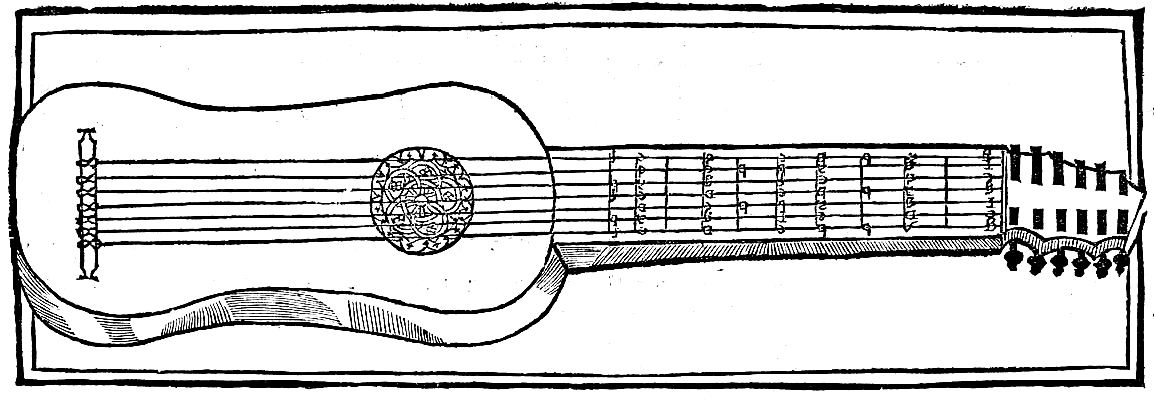
\includegraphics[width=\linewidth]{Bermudo-vihuela7}
\end{figure}
%}}}4

Indeed, vihuelas had been an important part of the Spanish royal musical ensemble
from the days of Charles I.
Vihuela intabulations survive of masses by Cristóbal de Morales and Francisco
Guerrero.%
    \Autocite[\sv{vihuela}]{Grove}
Vihuelas were almost certainly part of Cáseda's ensemble in Zaragoza, since the
instrument is mentioned frequently in the cathedral chapter acts.%
    \Autocite{Calahorra:Zaragoza2}
In Puebla, the cathedral chapter paid 100 pesos to one Diego de León in 1676
for playing the \term{vihuela de arco}, demonstrating the use of vihuelas in
the cathedral and suggesting their use as well in the closely related musical
ensemble of the Convento de la Santísima Trinidad.%
    \Autocite[44]{PerezRuiz:Aportes}

\index{Madrid!Royal Chapel}
\index{Charles I}
\index{Morales, Cristóbal de}
\index{Guerrero, Francisco}
\index{intabulation}
\index{villancico!scoring}
\index{Puebla!Convento de la Santísima Trinidad}

We know that women religious played the vihuela because one of the two
surviving vihuelas from this period, in the church of La Compañia de Jesús in
Quito, Ecuador, is believed to have been the possession of the nun Santa
Mariana de Jesús (1618--1645).
According to contemporary accounts, Mariana was especially skilled on the
instrument. 
The theological worth then attributed to the vihuela is shown in an account of
one Christmas night (probably during Matins service), when Mariana \quoted{sat
down to make music playing a vihuela, and she said that she wanted to offer
this music among the angels who were attending there}.%
\begin{Footnote}
    \Autocite[275]{EspinosaPolit:SantaMariana}, quoted in
    \Autocite[73]{Bermudez:Vihuela}.
\end{Footnote}
This form of devotional performance fits well with the original meaning of the
\foreign{kitharōdos} in \scripture{Rev 14}, \quoted{lyre-player, harpist who
plays an accompaniment to his own singing}.%
    \Autocite[\sv{kitharōdos}]{BDAG}
It is likely that the nuns of La Santísima Trinidad in Puebla also included at
least one vihuela in their musical ensemble.
It would seem strange for them not to use that instrument in performing a
villancico that used it as a metaphor for Christ (though the example of
\term{clarín} villancicos discussed in \chapref{ch:intro} suggests that an
instrument invoked symbolically need not be physically present).

\index{convent music}
\index{Quito}
\index{\emph{clarín}}

In Cáseda's villancico, the specific details of the vihuela---its construction,
tuning, playing technique, and typical stylistic idioms---provide new
allegorical possibilities for the poet to extend the cithara tradition.
More importantly, this poetic conceit of Christ as vihuela also provides Cáseda
as a composer with possibilites for actually representing the cithara symbol
through sound.
%}}}3
%}}}2

%{{{2 music
\subsection{Representing the Vihuela, Representing Christ}

In the poetry of Cáseda's villancico, the specifications of the vihuela become
symbols for Christ, particularly for his body, which suffered on the cross, was
raised, and became present to believers through the Eucharist.
The vihuela's seven strings here symbolize the seven sacraments.
According to Bermudo, the most common tuning for the seven strings was in
intervals of alternating fifths and fourths starting from a lowest string on 
\term{G (gamma, ut)}, that is, \pitch{G}{2}.%
    \Autocite[\folios{109\recto--109\verso}]{Bermudo:Declaracion}
That would make the strings \pitch{G}{2}, \pitch{D}{3}, \pitch{G}{3},
\pitch{D}{4}, \pitch{G}{4}, \pitch{D}{5}, \pitch{G}{5}.
Thus the highest and lowest strings are tuned in octaves, as copla 1 says:
\foreign{forma unida la alta con la baja}.
All the strings are tuned in perfect intervals, which may be part of the
meaning in copla 2, \foreign{en cada punto entera consonancia} (in each point
or note a whole consonance).
The \foreign{lazo} could refer either to the bow of a \term{vihuela de arco},
or to a plectrum that was sometimes used in place of the fingertips.
The poet has even incorporated the instrumental symbolism into the structure of
the verse, as the poem itself is composed primarily in lines of 7 and 11
syllables, beginning with the pattern 7--7--7--11--11---a pattern known as a
\term{lira}.%
    \Autocite{Lauer:Metrification}

\index{tuning}

Whether or not an actual vihuela was used for this villancico, Cáseda
represents the vihuela musically through the compositional structure.
First, he features the continuo section prominently, spotlighting all the
cithara-like instruments that might have been played.
The piece begins with the Tiple I (sister Tomasita in Puebla) singing a solo
against the continuo with widely-spaced open fifths and octaves between them.
The vihuela or other continuo instruments filling in the intervening space
would have stood out clearly.
Again in \measure{2}, when the Tiple I makes the striking leap up to the
B flat, she is joined only by the continuo.
In \measure{13}, there is an abrupt harmonic shift initiated by the continuo
alone, which here leads the singers rather than just accompanying them.

\index{performers!women}

Cáseda also gives the continuo several solos throughout the piece.
The first solo comes at the conclusion of the first three lines of poetry
(\measure{9}).
Surely the composer intended for more music to sound here than simply the
falling fifth of the melodic bass line.
Indeed, with the vocalists having just sung that the \quoted{divine music
\Dots{} rivals that of the birds}, it would seem natural for an instrumentalist
to fill in a little trilling bird music here.
Cáseda allows more possibilities in the coplas (\measures{52, 54, 57, 72,
76--77, 80}): in the first example, the ensemble sings \quoted{let the divine
strings resound}, and then there are two semiminims of vocal rest while the
continuo ensemble can do just that.

\index{musical topics!birdsong}

Cáseda also has the singers themselves imitate the vihuela.
In the opening gesture, the Tiple I sings her solo with continuo accompaniment,
followed by the rest of the vocal ensemble in a homorhythmic echo
(\musref{mus:CasedaJ-Que_musica_divina-opening}).
The chord voicing resembles the tuning of a vihuela, with the open fifths and
fourths in the three lower vocal parts of \measures{1--2}.
The dotted rhythm, sung all together, and the contrary motion between voices,
mimic the effect of strummed open strings on a vihuela.
The general texture of soloist against a regular rhythmic, chordal
accompaniment also evokes someone singing while playing (like Santa Mariana de
Jesús of Quito, and the \foreign{citharoedi} of \scripture{Rev 14}).
This image would be even clearer in the coplas sung by soloists with only
continuo accompaniment.

\index{musical topics!\emph{vihuela} music}
\index{imitation}

%{{{4 Caseda music opening
\begin{musicexample}
    \caption{Cáseda, \wtitle{Qúe música divina}, estribillo, opening}
    \label{mus:CasedaJ-Que_musica_divina-opening}
    \includefloat{CasedaJ-Que_musica_divina-opening}
\end{musicexample}
%}}}4

The vocal textures from \measure{6} on are more typical of vocal music,
particularly in the paired, ornament-like figures in the sections from
\measures{11--15, 19--39}.
After \measure{19}, Cáseda realizes the common villancico poetic trope of
birdsong by giving the singers birdlike trill patterns. 
At the end of the estribillo, Cáseda returns to musically representing the
vihuela/cithara trope.
In the last eight measures (\measures{47--50}), the rhythmic pattern in the
voices---a minim rest and two minims---again suggests strumming (see
\musref{mus:CasedaJ-Que_musica_divina-clausulas} below).
The estribillo ends with an alternating pattern of minor chords on G and
seventh chords over D, like the strumming of the two common vihuela chords,
known to us as \term{i} and \term{V\textsuperscript{7}}.
If this passage were played by a vihuelist in an intabulation, the player would
likely use a down-up-up strumming pattern, similar to the patterns recommended
for guitarists and harpists in Lucas Ruiz de Ribayaz's manual \wtitle{Luz y
norte musical} of 1677 (\figref{fig:Ruiz-strumming}).%
    \Autocite[9]{Ruiz:Luz}
In this rhythmic pattern, Cáseda inserts rests between syllables of the words
in this passage, and this rhetorical technique of \wtitle{tmesis} creates the
gasping effect of \quoted{dismayed}, arrested senses.

\index{Ruiz de Ribayaz, Lucas}
\index{rhetoric}

%{{{4 Ruiz strumming
\begin{figure}
    \caption{Strumming patterns in Ruiz de Ribayaz, \wtitle{Luz y norte
    musical}} 
    \label{fig:Ruiz-strumming}
    \includefloat{Ruiz-strumming}
\end{figure}
%}}}4

In the coplas, the homorhythmic, dotted opening phrase again seems to mimic
strumming.
For the phrase \foreign{forma unida la alta con la baja} (\measures{90--94}),
Cáseda sets the text on multiple levels at once.
In \measures{90--91}, the Tenor sings a pedal \pitch{D}{4}, like a droning open
string, against the Alto's moving line.
Thus the \foreign{alta} Alto is paired with the lowest voice.
The Tenor, meanwhile, forms perfect consonances (octave and fifth) with the
Bass, where a viheula on that part would likely be playing open D and G strings. 
The Tenor is thus acting like one of the strings on the vihuela.
All of these ideas are then repeated in the next phrase, \measures{92--93}, now
with G pedals, as though switching over to a different pair of strings.

These evocations of the vihuela would seem to fit with Hollander's thesis that
early modern poets shifted their interest from speculative views of music based
on ancient sources toward the details of practical contemporary music.
But in this case the tuning and performance practice of the contemporary
vihuela are harnessed as tools for theological allegory, more powerful in their
specificity than the vague term \term{cithara}.
In classic Neoplatonic fashion, the piece shows listeners how to hear
\wtitle{musica instrumentalis} while listening for the higher Music of Christ. 
The real, sounding vihuela is only a symbol of Christ.
It is Christ's musical \quoted{excellence} that is praised, not that of any
human virtuosi.

\index{Neoplatonism}
\index{\emph{musica instrumentalis}}
%}}}2

%{{{2 false music
\subsection{False Music}

\quoted{Of faith he is the intrument}, Cáseda's poem says of Christ,
\quoted{and his music regales the ear \add{or, hearing}} (copla 2).
That music, the poem says, is Christ's death on the cross.
But, as copla 5 says, \quoted{those things that his sovereign voices \add{or,
words} sound are not for the senses}.
This phrase (\foreign{no son a los sentidos}) echoes Thomas Aquinas's
description of the Eucharist: \quoted{That the true body of Christ and his
blood are in this sacrament, cannot be grasped by sensation \addorig{neque sensu}
nor by intellect, but by faith alone, which rests on divine authority}.% 
    \Autocite[question 75, article 1, \pagenum{274}]{Aquinas:Summa3}
When the villancico says, \quoted{sensation does not eat it} (\poemline{33}),
it recalls Aquinas's explanation that Christ's body is eaten in a sacramental,
not literally physical way.
Like the contests of the senses in \chapref{ch:faith-hearing}, this villancico
challenges the credibility of sensation even while appealing to it.
It prompts hearers to listen past what their ears perceive to grasp a higher
truth.
The real music of Christ's passion surpassed human understanding: in the words
of the villancico, \quoted{as many voices as the senses perceived from this
instrument will be false} or out of tune.
All this seems to be a way of saying in line with Aquinas that those who rely
on their senses, understood through reason alone, to grasp the mystery of
Christ in the Eucharist will fail.
Like Calderón's \quoted{Judaísmo} (\chapref{ch:faith-hearing}), they would be
hearing Faith without faith.

\index{Aquinas, Thomas}
\index{senses!limitations}
\index{tuning}
\index{doubt}
\index{harmony}
\index{Christ!as musician}

The reason why the music played on Christ the vihuela sounds \quoted{false} is
that in his crucifixion Christ is taking on humanity's sinful nature in order
to create harmony between humanity and God.
Here we see an intensified version of the dissonance trope in
\wtitle{Suspended, cielos} by Cererols: music that breaks earthly rules points
to \quoted{the new consonance} created by Christ.
Cáseda's villancico allows listeners to contemplate that Music, the
\quoted{mysterious excellence} or \quoted{virtuosity} of Christ the divine
musician, which \quoted{elevates to the heavens the one who reaches it}.
Since Cáseda's music with its open fifths and strumming patterns effectively
turns the whole ensemble into a vihuela, the piece becomes an active exercise
in putting the human community in tune with Christ.

Cáseda's exercises in depicting musical \quoted{falsehood} go well beyond the
mild dissonance used by Cererols, though.
In his opening (\musref{mus:CasedaJ-Que_musica_divina-opening}), Cáseda writes
direct octaves between the voice and accompaniment (in the leap up to B flat,
\measures{2}), and emphasizes them by cutting out all the other voices.
In the next two measures, Cáseda sets the word \foreign{acorde} (tuneful) to
bald parallel fifths between outer voices.
Cáseda suspends the Alto's B flat, so that these fifths move into a dissonant
seventh sonority.

These contrapuntal solecisms are what Bermudo calls musical \foreign{falsedad}.
He gives specific examples of parallel fifths and octaves, comparing them to
\quoted{barbarism in grammar}.%
    \Autocite[\folio{128\verso}]{Bermudo:Declaracion} 
In condemning this error, which he says is common for beginners and
instrumentalists, Bermudo uses some of the same key terms as Cáseda's
villancico:
\begin{quoting}
    I want to say that there are those taken for musicians who have learned
    without a teacher and with much labor, and they are poorly equipped
    \addorig{son faltos}, and they know few principles.
    This pestilence is especially great for keyboard players.  
    This is what that outstanding musician of blessed memory, Cristóbal de
    Morales, told me once, that if what many organists played would be written
    out we would find great faults.  
    And he had good reason to say it: because they can play two octaves and two
    fifths and not perceive it \add{because of the organ's timbre}: while
    singing it they would recognize the falsehood \addorig{falsedad}.% 
        \Autocite[\folio{128\verso}]{Bermudo:Declaracion} 
\end{quoting}
Direct and even parallel fifths do indeed regularly in the notated examples of
vihuela harmonization.%
    \Autocite{Araujo-Mendonca:Vihuela}
Just as in popular guitar music today, the construction of the instrument made
linear voice leading more difficult than simply shifting hand positions to
create parallel motion, and this idiom suited the chord-based music typical of
the instrument.

\index{solecisms}
\index{organ}
\index{music theory}

Cáseda has his musicians create \quoted{false} music through \quoted{dangerous}
and even intentionally erroneous counterpoint.
In the section beginning in \measure{40}, Cáseda tries out \foreign{cláusulas
varias} (various cadences), creating an effect as though all the voices are  
continually trying to cadence (\musref{mus:CasedaJ-Que_musica_divina-clausulas}).
Each of the voices sings a typical cadential pattern, but at different times
and not quite aligning relative to the others.
The chromaticism becomes more acute as the passage continues, culminating in a
bizarre collision in \measures{53--55}.
The bottom four voices here on their own in \measure{36} would appear to be
cadencing on F, with the C in the Bass to move up by fourth and the cadential E
in the Tiple II to resolve up to F.
But the top voice seems determined to cadence on G, so that in the second minim
of \measure{53} the top voice is an augmented fourth above the Bass (F sharp
against C), while the Alto's E is made to seem dissonant even when by rights it
should not be.
In \measure{54} the voices manages to cadence on D, with the top voice settling
back down to F sharp, though the Tenor has re-entered just at this point to sing
an unprepared dissonant B flat over the Bass (making an augmented fifth against
the Tiple I's F sharp).

%{{{5 Caseda clausulas
\begin{musicexample}
    \caption{Cáseda, \wtitle{Qué música divina}, \measures{40--55}:
    Conflicting \quoted{cadences} and false \term{ficta}}
    \label{mus:CasedaJ-Que_musica_divina-clausulas}
    \includefloat{CasedaJ-Que_musica_divina-clausulas}
\end{musicexample}
%}}}5

The final section of the estribillo
(\musref{mus:CasedaJ-Que_musica_divina-desmaya}) continues in this direction,
as Cáseda's music evokes the poetic idea of \quoted{elevating the senses} and
\quoted{dismaying the \add{bodily} powers}.
He begins with a wedge pattern between the Tenor and the accompaniment, again
juxtaposing B flat (in the Bass) with F sharp (in the tenor).
Cáseda brings in the next two voices, each one singing one of the two patterns
already introduced: the Alto has the ascending line, and the Tiple 2 has the
descending one.
But their entrances are flipped from that of the Bass and Tenor, so a reverse
wedge is created.
As this is happening, in \measure{61}, the Tiple I enters from out of nowhere
with a high A, skipping down to what is apparently an F natural (based on the
F sharp specified at the beginning of the next measure).
The A creates a \musFig{\na6 \fl3} sonority: on its own it is an imperfect
consonance with the Bass, but against the E flat in the Tiple II it certainly
has the effect of elevating and dismaying, amplified by the direct fifths it
then forms with the Bass as it skips down to F.
As though to ensure that listeners did not think this a mistake, Cáseda repeats
the whole passage again in \measure{67}, though with the voices rearranged.

%{{{5 Caseda desmaya
\begin{musicexample}
    \caption{Cáseda, \wtitle{Qué música divina}, \measures{63--80}: Elevating
    the senses, dismaying the faculties; rhetorical \term{tmesis} as
    strumming}
    \label{mus:CasedaJ-Que_musica_divina-desmaya}
    \includefloat{CasedaJ-Que_musica_divina-desmaya}
\end{musicexample}
%}}}5

The practice of \term{musica ficta}, still widespread in the Spanish Empire,
depended on the singer's ability to recognize places where the written pitches
needed to be inflected.%
   \Autocite{Berger:Ficta} 
As Cáseda's villancico progresses it requires more and more improvised
accidentals, until it starts to become unclear how to apply the rules, such as
in the strange collision of cadences in \measures{53--55}.
The Tiple II might begin the last phrase (starting in \measure{34} on F),
singing the E as part of a cadential formula on F and therefore natural; but
when the cadence comes on D, an E flat might be preferable. 
Either option clashes with the notated F sharp in the Tiple I.
In \measures{69--70}, on \foreign{potencias desmaya}, the ficta situation becomes
actually impossible.
To maintain the fugal motive, the Tiple II would have to sing three minim B
flats and then a semibreve B natural, leading up to C.
But in the same place as the Tiple II B flats, the Tenor has a notated sharp
sign on the B (the only way of indicating B natural in this mode).
The accidental in the Tenor part is clearly a sharp, written in the same hand
and with the same ink as the rest of the music.
This creates a cross relation---in Spanish, a \foreign{falsa relación}---between
the B flat and B natural.

\index{\emph{musica ficta}}
\index{music theory}

Any educated musicians confronted with this score would attempt to \quoted{fix}
these problems (probably by singing all B naturals in the Tiple II).
But any solution chosen feels wrong.
Is the music supposed to sound out-of-tune?
How should musicians apply ficta, how to tune intervals, when the composer is
forcing them to break the traditional rules?
The music is false: it cannot be emended with the further falsehood of musica
ficta or anything else.
That this should happen most blatantly at the opening of the piece on the very
word \foreign{acorde} is significant.
The fifths recall the tuning of the vihuela's strings, and the kind of music
typically played on the instrument. 
They were also the very paradigm of bad musicianship and untuneful composition.

Pedro Cerone specifically warned composers not to write passages that would
tempt singers to add incorrect accidentals and \quoted{falsify} the music.
Cerone uses the terms \foreign{falsa} and \foreign{falsificar} at different
times to mean either \term{musica ficta} or \quoted{wrong} notes (as in
\quoted{false relations}).
In certain situations (of which he gives a notated example, shown in
\figref{fig:Cerone-false_cadences}), \quoted{the singer can easily add a sharp to
the fifth, thinking it to be a cadence \addorig{cláusula}: for he will see that
the notes are moving in the manner of a cadence, saying \term{Sol fa sol},
\term{Re ut re}, and so on, and raising the note he will make it become false
\addorig{falsa}, and very dissonant to the ear}.% 
    \Autocite[629]{Cerone:Melopeo}
This is precisely the kind of passage Cáseda has written in his setting of
\foreign{cláusulas varias}: the parts all have typical cadential patterns like
the ones Cerone describes, and the voices would be tempted to raise certain
pitches at the wrong times. 
As with the parallel fifths that Bermudo warned against, Cáseda appears to be
breaking the rules deliberately and with symbolic intent.

\index{Cerone, Pedro}
\index{performers!applying \emph{musica ficta}}

%{{{4 cerone false cadences 
\begin{figure}
    \caption{Melodic patterns \quoted{in danger of being falsified} (sung with
    improper ficta) in Cerone, \wtitle{El melopeo y maestro}, 629} 
    \label{fig:Cerone-false_cadences}
    \includefloat{Cerone-false_cadences}
\end{figure}
%}}}4

Through his musical falsehoods, Cáseda has pushed the Neoplatonic theology of
music to the point where earthly music, rather than attempting to reflect
heavenly perfection, even if only partially, now overtly highlights its own
falsehood.
The emphasis is shifting toward using music not to reflect heaven at all, but
to aim primarily at \quoted{elevating the senses} and \quoted{dismaying the
powers}.
The goal for the hearers is moving from intellectual contemplation to affective
experience.
This change need not be seen as part of a \quoted{disenchantment} process, as
Hollander portrays it, though.
In order for Cáseda's flaunting of contrapuntal rules to have meaning, the
rules must still be preserved.
Breaking them for expressive purposes (whether affective expression or symbolic
expression, as of the Neoplatonic imperfection of \wtitle{musica
instrumentalis}) actually reflects a continued faith in the validity of those
rules.
Cáseda is not disregarding the old musical-theological system, but rather
insisting upon it so strongly that he passes over a reasonable limit and seems
to contradict himself.
As the tradition of metamusical villancicos developed, there was an increased
demand for composers both to imitate the conventions established by
predecessors and to differentiate their own works in some way. 
At the same time the concept of imitation itself, as a musical-rhetorical
practice within a Neoplatonic framework, was changing.
The three villancicos studied in this chapter demonstrate the first kind of
imitation---that of influence and homage---because they manifest a certain
degree of strain as each successive composer pushes the tradition of musical
self-representation further towards a limit of intelligibility.

\index{imitation}
\index{villancico!listener response}
\index{secularization}
\index{Hollander, John}
\index{Neoplatonism}
\index{affects}
\index{counterpoint, symbolism}

In contrast to the metamusical villancicos by Gutiérrez de Padilla and
Cererols, Bruna and Ambiela's variants of \wtitle{Suban las voces al cielo}, by
contrast, are less focused on abstract levels of music like the music of the
spheres or the angels.
Instead they use human music-making as an analogy for the dynamics of spiritual
communion, self-offering, and intercessory prayer.
The ensemble of convent sisters who sang Cáseda's villancico in Puebla embodied
through their voices the structure and style of the vihuela, a performance that
in turn interpreted that instrument as a physical sign pointing to Christ's
sufferings.
The body of Christ on the cross, made present in the Eucharist, was thus linked
to the body of the instrument, manifested symbolically through the bodies of
these women who had offered themselves in devotion to Christ.

\index{Cáseda, José de|)}
\index{musical instruments, symbolism|)}
\index{\emph{vihuela}|)}
\index{performers!women}
%}}}2
%}}}1

%{{{1 conclusions to book
\section{Conclusions}

Villancicos about music challenged composers to use the craft of music to
communicate theological ideas about music itself.
They presented hearers with the opportunity to listen for higher forms of music
through sounding music.
This complex music required that listeners be equipped with the requisite
musical, poetic, and religious knowledge and aural training to interpret it.
In line with the idea that faith was a virtue by which believers shaped
their lives in the image of Christ the Word, Catholics sought to create a
community of faithful hearers---one in which both the message and the process
of teaching were controlled under the authority of the Church.

\index{hearing}
\index{community}

This was an idealized theological vision of both the Church and of listening,
in which reliable teachers communicate without difficulty to trusting hearers,
all in perfect concord with the Holy Spirit's voice speaking down through the
hierarchy of the Christian community.
Real life was never so pristine.
Even if we could transport ourselves to Puebla Cathedral in 1657 or Lleida in
1689 we would not be able to answer the question of whether parishioners really
heard villancicos with faith---even whether they actually listened at all.
But we do know what was presented to their ears, and that is music that
directly explored the power of music to shape faith.

\index{theology!ecclesiology}
\index{audiences}

Evocations of angelic fugues and planetary cadences, castanets and vihuelas,
prompted listeners to reflect on the connections between worldly sounds and
heavenly truth.
In other words, villancicos were musical theology, sounding embodiments of a
worldview in which the Divine suffused Creation, through which God's nature
could be revealed to those who had learned to listen with faith as the book of
nature was read aloud.
If we take villancicos seriously as expressions of faith, we must conclude that
Spaniards believed music in performance could bring concord to individuals and
the community, after the pattern of the heavens.
In other words, they actively brought together Boethius's three kinds of music.
At the same time we must ask from a more mundane perspective what social
factors motivated early modern Spaniards to reiterate this theological vision
of music so vigorously.

\index{musical theology}
\index{creation}
\index{Boethius}
\index{faith}

I would argue that the notion of social harmony posed a special appeal to
people living under the Spanish crown.
The century after Columbus had transformed the complexion of the empire.
In America the minority of pure-blooded Spaniards lived under a constant threat
of native and African uprising, and the heirs of the Aztec Empire and the Kongo
Kingdom had to navigate a colonial society in which they could only be
\term{indios} and \term{negros}.
In Iberia, too, the influx of Native American goods and African slaves, not to
mention the Aztec and Inca gold underwriting the Habsburgs' growing debts,
destabilized the social order.
The theft of land and enslavement of fellow human beings put strain on Spanish
religion as well, forcing Spaniards to justify themselves.
Ethnic villancicos seem the most obvious manifestation of imperial Spain's
struggle with difference, but they are only one way that music enabled
Spaniards to make sense of this colorful and chaotic new world.
Images of human society all united in harmony, of a diversity of voices moving
together not in unison but in counterpoint, reinforced the social hierarchy in
a way that must have given comfort to the ruling class of Spain, just as it
added to the fear and confusion of their colonial subjects.%
    \Autocites
    {Baker:Harmony}
    {Irving:Colonial}
    {Illari:Polychoral}
Every clarion call reminded them that God had ordained the structures of
worldly power, just as surely as the sun was the fourth planet around a
stationary earth.
Of course, in the decades after Galileo and Newton's discoveries, people were
becoming aware that the cosmology used to justify the old regime did not square
with empirical observation; but in Spain the response was to insist all the
more strongly on the beauty of the old worldview.
Even as Spaniards began to emphasize the imperfection of music and creation
toward the end of the seventeenth century, they still did so as part of a 
Neoplatonic conception.

\index{harmony!social}
\index{Native Americans}
\index{Africans}
\index{slavery}
\index{villancicos!ethnic}
\index{\emph{clarín}}
\index{Galilei, Galileo}
\index{Newton, Isaac}
\index{science}
\index{perfection}
\index{Neoplatonism}
\index{villancico!social functions!project political power}
\index{colonialism}
\index{cosmos}

At the same time, though, the villancicos we have studied do not all present a
simple picture of social conformity.
From the worldly thrill of \term{jácara} outlaw ballads to the expressions of
doubt and misunderstanding in the dialogues of the deaf, villancicos did invite
a degree of critical reflection on the Church's role in contemporary society.
They were not just impositions of dogma or diverting but meaningless doggerel.
They asked hearers to doubt their own experiences and to temper their sensation
with faith.
They asked people to listen with faith, for faith.
And through their appeals both to social cohesion and to personal affective
response and commitment, they exhorted people to move past simple belief into
lives of faithfulness.

\index{villancico!listener response}
\index{doubt}
\index{hearing!training}
\index{\emph{jácara}}
\index{deafness}

Still, given the depths of injustice and hypocrisy in the Spanish Church during
the era of slavery and colonialism, it is not hard to understand the critique
of Juan de la Cruz (\chapref{ch:faith-hearing}) that Spaniards had their ears so
full of sweet harmonies that they were deaf to the actual call of Christ.%
    \Autocite
    [\range{bk}{3}, \range{ch}{45}, \pagenum{425}]
    {JuandelaCruz:Subida}
Music could help faith come through hearing, but as the friar Antonio de
Azevedo warned, what was heard had to come from \quoted{the word of Christ},
and people needed to be equipped to understand and receive it.%
    \Autocite{Azevedo:Catecismo}
Otherwise \quoted{all is vanity and a chasing after wind}
(\scripture{Eccl 1:14}).
All the harps and shawms and polychoral counterpoint in imperial Spain
amounted to no more than \quoted{noisy gongs and clanging cymbals}
(\scripture{1Cor 13:1}) if they did convert hearers of the word into doers
(\scripture{Jas 1:22}).

\index{Juan de la Cruz}
\index{Azevedo, Antonio de}
\index{faithfulness}
\index{villancico!ethical value}
\index{theology!ethical}
%}}}1



\mybackmatter
\chapter{Bibliography}
\label{ch:biblio}

\defbibfilter{primary}{keyword=primary or keyword=catalog}
\defbibfilter{secondary}{not keyword=primary and not keyword=catalog} 

\section*{Primary Sources, Music Scores, and Catalogs}
\printbibliography[heading=none,filter=primary]

\section*{Secondary Scholarship}
\printbibliography[heading=none,filter=secondary]

\endinput





\printindex


\end{document}
